\documentclass[twoside]{book}

% Packages required by doxygen
\usepackage{fixltx2e}
\usepackage{calc}
\usepackage{doxygen}
\usepackage[export]{adjustbox} % also loads graphicx
\usepackage{graphicx}
\usepackage[utf8]{inputenc}
\usepackage{makeidx}
\usepackage{multicol}
\usepackage{multirow}
\PassOptionsToPackage{warn}{textcomp}
\usepackage{textcomp}
\usepackage[nointegrals]{wasysym}
\usepackage[table]{xcolor}

% Font selection
\usepackage[T1]{fontenc}
\usepackage[scaled=.90]{helvet}
\usepackage{courier}
\usepackage{amssymb}
\usepackage{sectsty}
\renewcommand{\familydefault}{\sfdefault}
\allsectionsfont{%
  \fontseries{bc}\selectfont%
  \color{darkgray}%
}
\renewcommand{\DoxyLabelFont}{%
  \fontseries{bc}\selectfont%
  \color{darkgray}%
}
\newcommand{\+}{\discretionary{\mbox{\scriptsize$\hookleftarrow$}}{}{}}

% Page & text layout
\usepackage{geometry}
\geometry{%
  a4paper,%
  top=2.5cm,%
  bottom=2.5cm,%
  left=2.5cm,%
  right=2.5cm%
}
\tolerance=750
\hfuzz=15pt
\hbadness=750
\setlength{\emergencystretch}{15pt}
\setlength{\parindent}{0cm}
\setlength{\parskip}{0.2cm}
\makeatletter
\renewcommand{\paragraph}{%
  \@startsection{paragraph}{4}{0ex}{-1.0ex}{1.0ex}{%
    \normalfont\normalsize\bfseries\SS@parafont%
  }%
}
\renewcommand{\subparagraph}{%
  \@startsection{subparagraph}{5}{0ex}{-1.0ex}{1.0ex}{%
    \normalfont\normalsize\bfseries\SS@subparafont%
  }%
}
\makeatother

% Headers & footers
\usepackage{fancyhdr}
\pagestyle{fancyplain}
\fancyhead[LE]{\fancyplain{}{\bfseries\thepage}}
\fancyhead[CE]{\fancyplain{}{}}
\fancyhead[RE]{\fancyplain{}{\bfseries\leftmark}}
\fancyhead[LO]{\fancyplain{}{\bfseries\rightmark}}
\fancyhead[CO]{\fancyplain{}{}}
\fancyhead[RO]{\fancyplain{}{\bfseries\thepage}}
\fancyfoot[LE]{\fancyplain{}{}}
\fancyfoot[CE]{\fancyplain{}{}}
\fancyfoot[RE]{\fancyplain{}{\bfseries\scriptsize Generated on Wed Apr 22 2015 17\+:25\+:28 for Platypus by Doxygen }}
\fancyfoot[LO]{\fancyplain{}{\bfseries\scriptsize Generated on Wed Apr 22 2015 17\+:25\+:28 for Platypus by Doxygen }}
\fancyfoot[CO]{\fancyplain{}{}}
\fancyfoot[RO]{\fancyplain{}{}}
\renewcommand{\footrulewidth}{0.4pt}
\renewcommand{\chaptermark}[1]{%
  \markboth{#1}{}%
}
\renewcommand{\sectionmark}[1]{%
  \markright{\thesection\ #1}%
}

% Indices & bibliography
\usepackage{natbib}
\usepackage[titles]{tocloft}
\setcounter{tocdepth}{3}
\setcounter{secnumdepth}{5}
\makeindex

% Hyperlinks (required, but should be loaded last)
\usepackage{ifpdf}
\ifpdf
  \usepackage[pdftex,pagebackref=true]{hyperref}
\else
  \usepackage[ps2pdf,pagebackref=true]{hyperref}
\fi
\hypersetup{%
  colorlinks=true,%
  linkcolor=blue,%
  citecolor=blue,%
  unicode%
}

% Custom commands
\newcommand{\clearemptydoublepage}{%
  \newpage{\pagestyle{empty}\cleardoublepage}%
}


%===== C O N T E N T S =====

\begin{document}

% Titlepage & ToC
\hypersetup{pageanchor=false,
             bookmarks=true,
             bookmarksnumbered=true,
             pdfencoding=unicode
            }
\pagenumbering{roman}
\begin{titlepage}
\vspace*{7cm}
\begin{center}%
{\Large Platypus \\[1ex]\large 1.\+0 }\\
\vspace*{1cm}
{\large Generated by Doxygen 1.8.9.1}\\
\vspace*{0.5cm}
{\small Wed Apr 22 2015 17:25:28}\\
\end{center}
\end{titlepage}
\clearemptydoublepage
\tableofcontents
\clearemptydoublepage
\pagenumbering{arabic}
\hypersetup{pageanchor=true}

%--- Begin generated contents ---
\chapter{Namespace Index}
\section{Namespace List}
Here is a list of all namespaces with brief descriptions\+:\begin{DoxyCompactList}
\item\contentsline{section}{{\bf manage} }{\pageref{namespacemanage}}{}
\item\contentsline{section}{{\bf match\+App} }{\pageref{namespacematch_app}}{}
\item\contentsline{section}{{\bf match\+App.\+admin} }{\pageref{namespacematch_app_1_1admin}}{}
\item\contentsline{section}{{\bf match\+App.\+forms} }{\pageref{namespacematch_app_1_1forms}}{}
\item\contentsline{section}{{\bf match\+App.\+matching\+Algorithm} }{\pageref{namespacematch_app_1_1matching_algorithm}}{}
\item\contentsline{section}{{\bf match\+App.\+matching\+Algorithm.\+add\+Course} }{\pageref{namespacematch_app_1_1matching_algorithm_1_1add_course}}{}
\item\contentsline{section}{{\bf match\+App.\+matching\+Algorithm.\+query\+And\+Match\+Courses} }{\pageref{namespacematch_app_1_1matching_algorithm_1_1query_and_match_courses}}{}
\item\contentsline{section}{{\bf match\+App.\+matching\+Algorithm.\+query\+And\+Match\+Sections} }{\pageref{namespacematch_app_1_1matching_algorithm_1_1query_and_match_sections}}{}
\item\contentsline{section}{{\bf match\+App.\+matching\+Algorithm.\+remove\+Course} }{\pageref{namespacematch_app_1_1matching_algorithm_1_1remove_course}}{}
\item\contentsline{section}{{\bf match\+App.\+matching\+Algorithm.\+return\+Course\+List} }{\pageref{namespacematch_app_1_1matching_algorithm_1_1return_course_list}}{}
\item\contentsline{section}{{\bf match\+App.\+matching\+Algorithm.\+return\+Matches\+By\+Course} }{\pageref{namespacematch_app_1_1matching_algorithm_1_1return_matches_by_course}}{}
\item\contentsline{section}{{\bf match\+App.\+matching\+Algorithm.\+return\+Matches\+By\+Section} }{\pageref{namespacematch_app_1_1matching_algorithm_1_1return_matches_by_section}}{}
\item\contentsline{section}{{\bf match\+App.\+matching\+Algorithm.\+return\+Sections\+List} }{\pageref{namespacematch_app_1_1matching_algorithm_1_1return_sections_list}}{}
\item\contentsline{section}{{\bf match\+App.\+matching\+Algorithm.\+return\+Student\+Data} }{\pageref{namespacematch_app_1_1matching_algorithm_1_1return_student_data}}{}
\item\contentsline{section}{{\bf match\+App.\+models} }{\pageref{namespacematch_app_1_1models}}{}
\item\contentsline{section}{{\bf match\+App.\+templatetags} }{\pageref{namespacematch_app_1_1templatetags}}{}
\item\contentsline{section}{{\bf match\+App.\+templatetags.\+dict\+\_\+helper} }{\pageref{namespacematch_app_1_1templatetags_1_1dict__helper}}{}
\item\contentsline{section}{{\bf match\+App.\+tests} }{\pageref{namespacematch_app_1_1tests}}{}
\item\contentsline{section}{{\bf match\+App.\+urls} }{\pageref{namespacematch_app_1_1urls}}{}
\item\contentsline{section}{{\bf match\+App.\+views} }{\pageref{namespacematch_app_1_1views}}{}
\item\contentsline{section}{{\bf Platypus} }{\pageref{namespace_platypus}}{}
\item\contentsline{section}{{\bf Platypus.\+settings} }{\pageref{namespace_platypus_1_1settings}}{}
\item\contentsline{section}{{\bf Platypus.\+urls} }{\pageref{namespace_platypus_1_1urls}}{}
\item\contentsline{section}{{\bf Platypus.\+wsgi} }{\pageref{namespace_platypus_1_1wsgi}}{}
\item\contentsline{section}{{\bf populate} }{\pageref{namespacepopulate}}{}
\end{DoxyCompactList}

\chapter{Hierarchical Index}
\section{Class Hierarchy}
This inheritance list is sorted roughly, but not completely, alphabetically\+:\begin{DoxyCompactList}
\item \contentsline{section}{match\+App.\+forms.\+User\+Form.\+Meta}{\pageref{classmatch_app_1_1forms_1_1_user_form_1_1_meta}}{}
\item Model\begin{DoxyCompactList}
\item \contentsline{section}{match\+App.\+models.\+Course}{\pageref{classmatch_app_1_1models_1_1_course}}{}
\item \contentsline{section}{match\+App.\+models.\+Section}{\pageref{classmatch_app_1_1models_1_1_section}}{}
\item \contentsline{section}{match\+App.\+models.\+Student}{\pageref{classmatch_app_1_1models_1_1_student}}{}
\end{DoxyCompactList}
\item Model\+Form\begin{DoxyCompactList}
\item \contentsline{section}{match\+App.\+forms.\+User\+Form}{\pageref{classmatch_app_1_1forms_1_1_user_form}}{}
\end{DoxyCompactList}
\end{DoxyCompactList}

\chapter{Class Index}
\section{Class List}
Here are the classes, structs, unions and interfaces with brief descriptions\+:\begin{DoxyCompactList}
\item\contentsline{section}{{\bf match\+App.\+models.\+Course} }{\pageref{classmatch_app_1_1models_1_1_course}}{}
\item\contentsline{section}{{\bf match\+App.\+forms.\+User\+Form.\+Meta} }{\pageref{classmatch_app_1_1forms_1_1_user_form_1_1_meta}}{}
\item\contentsline{section}{{\bf match\+App.\+models.\+Section} }{\pageref{classmatch_app_1_1models_1_1_section}}{}
\item\contentsline{section}{{\bf match\+App.\+models.\+Student} }{\pageref{classmatch_app_1_1models_1_1_student}}{}
\item\contentsline{section}{{\bf match\+App.\+forms.\+User\+Form} }{\pageref{classmatch_app_1_1forms_1_1_user_form}}{}
\end{DoxyCompactList}

\chapter{File Index}
\section{File List}
Here is a list of all files with brief descriptions\+:\begin{DoxyCompactList}
\item\contentsline{section}{{\bf manage.\+py} }{\pageref{manage_8py}}{}
\item\contentsline{section}{{\bf populate.\+py} }{\pageref{populate_8py}}{}
\item\contentsline{section}{match\+App/{\bf \+\_\+\+\_\+init\+\_\+\+\_\+.\+py} }{\pageref{match_app_2____init_____8py}}{}
\item\contentsline{section}{match\+App/{\bf admin.\+py} }{\pageref{admin_8py}}{}
\item\contentsline{section}{match\+App/{\bf forms.\+py} }{\pageref{forms_8py}}{}
\item\contentsline{section}{match\+App/{\bf models.\+py} \\*Django models organizes classes used for the application }{\pageref{models_8py}}{}
\item\contentsline{section}{match\+App/{\bf tests.\+py} }{\pageref{tests_8py}}{}
\item\contentsline{section}{match\+App/{\bf urls.\+py} }{\pageref{match_app_2urls_8py}}{}
\item\contentsline{section}{match\+App/{\bf views.\+py} }{\pageref{views_8py}}{}
\item\contentsline{section}{match\+App/html/{\bf dynsections.\+js} }{\pageref{dynsections_8js}}{}
\item\contentsline{section}{match\+App/html/{\bf jquery.\+js} }{\pageref{jquery_8js}}{}
\item\contentsline{section}{match\+App/html/search/{\bf all\+\_\+0.\+js} }{\pageref{all__0_8js}}{}
\item\contentsline{section}{match\+App/html/search/{\bf all\+\_\+1.\+js} }{\pageref{all__1_8js}}{}
\item\contentsline{section}{match\+App/html/search/{\bf all\+\_\+2.\+js} }{\pageref{all__2_8js}}{}
\item\contentsline{section}{match\+App/html/search/{\bf all\+\_\+3.\+js} }{\pageref{all__3_8js}}{}
\item\contentsline{section}{match\+App/html/search/{\bf all\+\_\+4.\+js} }{\pageref{all__4_8js}}{}
\item\contentsline{section}{match\+App/html/search/{\bf all\+\_\+5.\+js} }{\pageref{all__5_8js}}{}
\item\contentsline{section}{match\+App/html/search/{\bf all\+\_\+6.\+js} }{\pageref{all__6_8js}}{}
\item\contentsline{section}{match\+App/html/search/{\bf classes\+\_\+0.\+js} }{\pageref{classes__0_8js}}{}
\item\contentsline{section}{match\+App/html/search/{\bf classes\+\_\+1.\+js} }{\pageref{classes__1_8js}}{}
\item\contentsline{section}{match\+App/html/search/{\bf classes\+\_\+2.\+js} }{\pageref{classes__2_8js}}{}
\item\contentsline{section}{match\+App/html/search/{\bf classes\+\_\+3.\+js} }{\pageref{classes__3_8js}}{}
\item\contentsline{section}{match\+App/html/search/{\bf files\+\_\+0.\+js} }{\pageref{files__0_8js}}{}
\item\contentsline{section}{match\+App/html/search/{\bf functions\+\_\+0.\+js} }{\pageref{functions__0_8js}}{}
\item\contentsline{section}{match\+App/html/search/{\bf functions\+\_\+1.\+js} }{\pageref{functions__1_8js}}{}
\item\contentsline{section}{match\+App/html/search/{\bf functions\+\_\+2.\+js} }{\pageref{functions__2_8js}}{}
\item\contentsline{section}{match\+App/html/search/{\bf functions\+\_\+3.\+js} }{\pageref{functions__3_8js}}{}
\item\contentsline{section}{match\+App/html/search/{\bf functions\+\_\+4.\+js} }{\pageref{functions__4_8js}}{}
\item\contentsline{section}{match\+App/html/search/{\bf namespaces\+\_\+0.\+js} }{\pageref{namespaces__0_8js}}{}
\item\contentsline{section}{match\+App/html/search/{\bf search.\+js} }{\pageref{search_8js}}{}
\item\contentsline{section}{match\+App/html/search/{\bf searchdata.\+js} }{\pageref{searchdata_8js}}{}
\item\contentsline{section}{match\+App/matching\+Algorithm/{\bf \+\_\+\+\_\+init\+\_\+\+\_\+.\+py} }{\pageref{match_app_2matching_algorithm_2____init_____8py}}{}
\item\contentsline{section}{match\+App/matching\+Algorithm/{\bf add\+Course.\+py} }{\pageref{add_course_8py}}{}
\item\contentsline{section}{match\+App/matching\+Algorithm/{\bf query\+And\+Match\+Courses.\+py} }{\pageref{query_and_match_courses_8py}}{}
\item\contentsline{section}{match\+App/matching\+Algorithm/{\bf query\+And\+Match\+Sections.\+py} }{\pageref{query_and_match_sections_8py}}{}
\item\contentsline{section}{match\+App/matching\+Algorithm/{\bf remove\+Course.\+py} }{\pageref{remove_course_8py}}{}
\item\contentsline{section}{match\+App/matching\+Algorithm/{\bf return\+Course\+List.\+py} }{\pageref{return_course_list_8py}}{}
\item\contentsline{section}{match\+App/matching\+Algorithm/{\bf return\+Matches\+By\+Course.\+py} }{\pageref{return_matches_by_course_8py}}{}
\item\contentsline{section}{match\+App/matching\+Algorithm/{\bf return\+Matches\+By\+Section.\+py} }{\pageref{return_matches_by_section_8py}}{}
\item\contentsline{section}{match\+App/matching\+Algorithm/{\bf return\+Sections\+List.\+py} }{\pageref{return_sections_list_8py}}{}
\item\contentsline{section}{match\+App/matching\+Algorithm/{\bf return\+Student\+Data.\+py} }{\pageref{return_student_data_8py}}{}
\item\contentsline{section}{match\+App/templatetags/{\bf \+\_\+\+\_\+init\+\_\+\+\_\+.\+py} }{\pageref{match_app_2templatetags_2____init_____8py}}{}
\item\contentsline{section}{match\+App/templatetags/{\bf dict\+\_\+helper.\+py} }{\pageref{dict__helper_8py}}{}
\item\contentsline{section}{Platypus/{\bf \+\_\+\+\_\+init\+\_\+\+\_\+.\+py} }{\pageref{_platypus_2____init_____8py}}{}
\item\contentsline{section}{Platypus/{\bf settings.\+py} }{\pageref{settings_8py}}{}
\item\contentsline{section}{Platypus/{\bf urls.\+py} }{\pageref{_platypus_2urls_8py}}{}
\item\contentsline{section}{Platypus/{\bf wsgi.\+py} }{\pageref{wsgi_8py}}{}
\item\contentsline{section}{static/bootstrap/js/{\bf bootstrap.\+js} }{\pageref{bootstrap_8js}}{}
\item\contentsline{section}{static/bootstrap/js/{\bf bootstrap.\+min.\+js} }{\pageref{bootstrap_8min_8js}}{}
\item\contentsline{section}{static/bootstrap/js/{\bf npm.\+js} }{\pageref{npm_8js}}{}
\end{DoxyCompactList}

\chapter{Namespace Documentation}
\hypertarget{namespacemanage}{}\section{manage Namespace Reference}
\label{namespacemanage}\index{manage@{manage}}

\hypertarget{namespacematch_app}{}\section{match\+App Namespace Reference}
\label{namespacematch_app}\index{match\+App@{match\+App}}
\subsection*{Namespaces}
\begin{DoxyCompactItemize}
\item 
 \hyperlink{namespacematch_app_1_1admin}{admin}
\item 
 \hyperlink{namespacematch_app_1_1forms}{forms}
\item 
 \hyperlink{namespacematch_app_1_1matching_algorithm}{matching\+Algorithm}
\item 
 \hyperlink{namespacematch_app_1_1models}{models}
\item 
 \hyperlink{namespacematch_app_1_1templatetags}{templatetags}
\item 
 \hyperlink{namespacematch_app_1_1tests}{tests}
\item 
 \hyperlink{namespacematch_app_1_1urls}{urls}
\item 
 \hyperlink{namespacematch_app_1_1views}{views}
\end{DoxyCompactItemize}

\hypertarget{namespacematch_app_1_1admin}{}\section{match\+App.\+admin Namespace Reference}
\label{namespacematch_app_1_1admin}\index{match\+App.\+admin@{match\+App.\+admin}}

\hypertarget{namespacematch_app_1_1forms}{}\section{match\+App.\+forms Namespace Reference}
\label{namespacematch_app_1_1forms}\index{match\+App.\+forms@{match\+App.\+forms}}
\subsection*{Classes}
\begin{DoxyCompactItemize}
\item 
class \hyperlink{classmatch_app_1_1forms_1_1_user_form}{User\+Form}
\end{DoxyCompactItemize}


\subsection{Detailed Description}
\begin{DoxyVerb}forms for taking input from users\end{DoxyVerb}
 
\hypertarget{namespacematch_app_1_1matching_algorithm}{}\section{match\+App.\+matching\+Algorithm Namespace Reference}
\label{namespacematch_app_1_1matching_algorithm}\index{match\+App.\+matching\+Algorithm@{match\+App.\+matching\+Algorithm}}
\subsection*{Namespaces}
\begin{DoxyCompactItemize}
\item 
 \hyperlink{namespacematch_app_1_1matching_algorithm_1_1add_course}{add\+Course}
\item 
 \hyperlink{namespacematch_app_1_1matching_algorithm_1_1query_and_match_courses}{query\+And\+Match\+Courses}
\item 
 \hyperlink{namespacematch_app_1_1matching_algorithm_1_1query_and_match_sections}{query\+And\+Match\+Sections}
\item 
 \hyperlink{namespacematch_app_1_1matching_algorithm_1_1remove_course}{remove\+Course}
\item 
 \hyperlink{namespacematch_app_1_1matching_algorithm_1_1return_course_list}{return\+Course\+List}
\item 
 \hyperlink{namespacematch_app_1_1matching_algorithm_1_1return_matches_by_course}{return\+Matches\+By\+Course}
\item 
 \hyperlink{namespacematch_app_1_1matching_algorithm_1_1return_matches_by_section}{return\+Matches\+By\+Section}
\item 
 \hyperlink{namespacematch_app_1_1matching_algorithm_1_1return_sections_list}{return\+Sections\+List}
\item 
 \hyperlink{namespacematch_app_1_1matching_algorithm_1_1return_student_data}{return\+Student\+Data}
\end{DoxyCompactItemize}

\section{match\+App.\+matching\+Algorithm.\+add\+Course Namespace Reference}
\label{namespacematch_app_1_1matching_algorithm_1_1add_course}\index{match\+App.\+matching\+Algorithm.\+add\+Course@{match\+App.\+matching\+Algorithm.\+add\+Course}}
\subsection*{Functions}
\begin{DoxyCompactItemize}
\item 
def {\bf add\+Course} (student\+\_\+id, section\+\_\+id)
\end{DoxyCompactItemize}
\subsection*{Variables}
\begin{DoxyCompactItemize}
\item 
tuple {\bf directory} = os.\+getcwd()
\begin{DoxyCompactList}\small\item\em Append parent of the parent directory for cwd to system path \#. \end{DoxyCompactList}\end{DoxyCompactItemize}


\subsection{Detailed Description}
\begin{DoxyVerb}Allows a student to add a course \end{DoxyVerb}
 

\subsection{Function Documentation}
\index{match\+App\+::matching\+Algorithm\+::add\+Course@{match\+App\+::matching\+Algorithm\+::add\+Course}!add\+Course@{add\+Course}}
\index{add\+Course@{add\+Course}!match\+App\+::matching\+Algorithm\+::add\+Course@{match\+App\+::matching\+Algorithm\+::add\+Course}}
\subsubsection[{add\+Course}]{\setlength{\rightskip}{0pt plus 5cm}def match\+App.\+matching\+Algorithm.\+add\+Course.\+add\+Course (
\begin{DoxyParamCaption}
\item[{}]{student\+\_\+id, }
\item[{}]{section\+\_\+id}
\end{DoxyParamCaption}
)}\label{namespacematch_app_1_1matching_algorithm_1_1add_course_ae931314b031acb961c8d3f2fa6c4b338}
\begin{DoxyVerb}Function to add a course to be available on Platypus. 
Arguments: student_id, and section_id of the course to be added 
Saves course to database. \end{DoxyVerb}
 

\subsection{Variable Documentation}
\index{match\+App\+::matching\+Algorithm\+::add\+Course@{match\+App\+::matching\+Algorithm\+::add\+Course}!directory@{directory}}
\index{directory@{directory}!match\+App\+::matching\+Algorithm\+::add\+Course@{match\+App\+::matching\+Algorithm\+::add\+Course}}
\subsubsection[{directory}]{\setlength{\rightskip}{0pt plus 5cm}tuple match\+App.\+matching\+Algorithm.\+add\+Course.\+directory = os.\+getcwd()}\label{namespacematch_app_1_1matching_algorithm_1_1add_course_a6e7c3f074c5f1319de59da69820f345d}


Append parent of the parent directory for cwd to system path \#. 


\section{match\+App.\+matching\+Algorithm.\+query\+And\+Match\+Courses Namespace Reference}
\label{namespacematch_app_1_1matching_algorithm_1_1query_and_match_courses}\index{match\+App.\+matching\+Algorithm.\+query\+And\+Match\+Courses@{match\+App.\+matching\+Algorithm.\+query\+And\+Match\+Courses}}
\subsection*{Functions}
\begin{DoxyCompactItemize}
\item 
def {\bf query\+And\+Match\+Courses} ()
\end{DoxyCompactItemize}
\subsection*{Variables}
\begin{DoxyCompactItemize}
\item 
tuple {\bf directory} = os.\+getcwd()
\end{DoxyCompactItemize}


\subsection{Detailed Description}
\begin{DoxyVerb}Organizes information from database according to students and their courses\end{DoxyVerb}
 

\subsection{Function Documentation}
\index{match\+App\+::matching\+Algorithm\+::query\+And\+Match\+Courses@{match\+App\+::matching\+Algorithm\+::query\+And\+Match\+Courses}!query\+And\+Match\+Courses@{query\+And\+Match\+Courses}}
\index{query\+And\+Match\+Courses@{query\+And\+Match\+Courses}!match\+App\+::matching\+Algorithm\+::query\+And\+Match\+Courses@{match\+App\+::matching\+Algorithm\+::query\+And\+Match\+Courses}}
\subsubsection[{query\+And\+Match\+Courses}]{\setlength{\rightskip}{0pt plus 5cm}def match\+App.\+matching\+Algorithm.\+query\+And\+Match\+Courses.\+query\+And\+Match\+Courses (
\begin{DoxyParamCaption}
{}
\end{DoxyParamCaption}
)}\label{namespacematch_app_1_1matching_algorithm_1_1query_and_match_courses_ad9a21ebabe891164c9f7639c6358ae7c}
\begin{DoxyVerb}Create a hashtable that saves course numbers as keys and arrays of enrolled students as values. 
Query all sections in the database.
Save each section number from course_list string into an array.
Extract department ID and first four chars of section id.
Returns the course dictionary.
\end{DoxyVerb}
 

\subsection{Variable Documentation}
\index{match\+App\+::matching\+Algorithm\+::query\+And\+Match\+Courses@{match\+App\+::matching\+Algorithm\+::query\+And\+Match\+Courses}!directory@{directory}}
\index{directory@{directory}!match\+App\+::matching\+Algorithm\+::query\+And\+Match\+Courses@{match\+App\+::matching\+Algorithm\+::query\+And\+Match\+Courses}}
\subsubsection[{directory}]{\setlength{\rightskip}{0pt plus 5cm}tuple match\+App.\+matching\+Algorithm.\+query\+And\+Match\+Courses.\+directory = os.\+getcwd()}\label{namespacematch_app_1_1matching_algorithm_1_1query_and_match_courses_a0bd38294da3bda8051731c034f1de149}

\hypertarget{namespacematch_app_1_1matching_algorithm_1_1query_and_match_sections}{}\section{match\+App.\+matching\+Algorithm.\+query\+And\+Match\+Sections Namespace Reference}
\label{namespacematch_app_1_1matching_algorithm_1_1query_and_match_sections}\index{match\+App.\+matching\+Algorithm.\+query\+And\+Match\+Sections@{match\+App.\+matching\+Algorithm.\+query\+And\+Match\+Sections}}
\subsection*{Functions}
\begin{DoxyCompactItemize}
\item 
def \hyperlink{namespacematch_app_1_1matching_algorithm_1_1query_and_match_sections_a3e86e2d2e95ae60932642651aaddfdd2}{query\+And\+Match\+Sections} ()
\end{DoxyCompactItemize}
\subsection*{Variables}
\begin{DoxyCompactItemize}
\item 
tuple \hyperlink{namespacematch_app_1_1matching_algorithm_1_1query_and_match_sections_a1fb8589712b684c335ad24e499b445fa}{directory} = os.\+getcwd()
\end{DoxyCompactItemize}


\subsection{Detailed Description}
\begin{DoxyVerb}Organizes information from the database according to students and their specific sections of courses.\end{DoxyVerb}
 

\subsection{Function Documentation}
\hypertarget{namespacematch_app_1_1matching_algorithm_1_1query_and_match_sections_a3e86e2d2e95ae60932642651aaddfdd2}{}\index{match\+App\+::matching\+Algorithm\+::query\+And\+Match\+Sections@{match\+App\+::matching\+Algorithm\+::query\+And\+Match\+Sections}!query\+And\+Match\+Sections@{query\+And\+Match\+Sections}}
\index{query\+And\+Match\+Sections@{query\+And\+Match\+Sections}!match\+App\+::matching\+Algorithm\+::query\+And\+Match\+Sections@{match\+App\+::matching\+Algorithm\+::query\+And\+Match\+Sections}}
\subsubsection[{query\+And\+Match\+Sections}]{\setlength{\rightskip}{0pt plus 5cm}def match\+App.\+matching\+Algorithm.\+query\+And\+Match\+Sections.\+query\+And\+Match\+Sections (
\begin{DoxyParamCaption}
{}
\end{DoxyParamCaption}
)}\label{namespacematch_app_1_1matching_algorithm_1_1query_and_match_sections_a3e86e2d2e95ae60932642651aaddfdd2}
\begin{DoxyVerb}Create a hashtable that saves section numbers as keys and arrays of enrolled students as values. 
Querey all rows in the section and student tables. Add the student ID to to the array hashed by the directory for each course
in which the student is enrolled. 
Return a dictionary of the sections. 
\end{DoxyVerb}
 

\subsection{Variable Documentation}
\hypertarget{namespacematch_app_1_1matching_algorithm_1_1query_and_match_sections_a1fb8589712b684c335ad24e499b445fa}{}\index{match\+App\+::matching\+Algorithm\+::query\+And\+Match\+Sections@{match\+App\+::matching\+Algorithm\+::query\+And\+Match\+Sections}!directory@{directory}}
\index{directory@{directory}!match\+App\+::matching\+Algorithm\+::query\+And\+Match\+Sections@{match\+App\+::matching\+Algorithm\+::query\+And\+Match\+Sections}}
\subsubsection[{directory}]{\setlength{\rightskip}{0pt plus 5cm}tuple match\+App.\+matching\+Algorithm.\+query\+And\+Match\+Sections.\+directory = os.\+getcwd()}\label{namespacematch_app_1_1matching_algorithm_1_1query_and_match_sections_a1fb8589712b684c335ad24e499b445fa}

\section{match\+App.\+matching\+Algorithm.\+remove\+Course Namespace Reference}
\label{namespacematch_app_1_1matching_algorithm_1_1remove_course}\index{match\+App.\+matching\+Algorithm.\+remove\+Course@{match\+App.\+matching\+Algorithm.\+remove\+Course}}
\subsection*{Functions}
\begin{DoxyCompactItemize}
\item 
def {\bf remove\+Course} (student\+\_\+id, section\+\_\+id)
\item 
def {\bf main} ()
\end{DoxyCompactItemize}
\subsection*{Variables}
\begin{DoxyCompactItemize}
\item 
tuple {\bf directory} = os.\+getcwd()
\begin{DoxyCompactList}\small\item\em Append parent of the parent directory for cwd to system path \#. \end{DoxyCompactList}\end{DoxyCompactItemize}


\subsection{Detailed Description}
\begin{DoxyVerb}Allows a student to remove a course from their course list\end{DoxyVerb}
 

\subsection{Function Documentation}
\index{match\+App\+::matching\+Algorithm\+::remove\+Course@{match\+App\+::matching\+Algorithm\+::remove\+Course}!main@{main}}
\index{main@{main}!match\+App\+::matching\+Algorithm\+::remove\+Course@{match\+App\+::matching\+Algorithm\+::remove\+Course}}
\subsubsection[{main}]{\setlength{\rightskip}{0pt plus 5cm}def match\+App.\+matching\+Algorithm.\+remove\+Course.\+main (
\begin{DoxyParamCaption}
{}
\end{DoxyParamCaption}
)}\label{namespacematch_app_1_1matching_algorithm_1_1remove_course_a7d407f5ed0323430f9118d99eedc2b82}
\index{match\+App\+::matching\+Algorithm\+::remove\+Course@{match\+App\+::matching\+Algorithm\+::remove\+Course}!remove\+Course@{remove\+Course}}
\index{remove\+Course@{remove\+Course}!match\+App\+::matching\+Algorithm\+::remove\+Course@{match\+App\+::matching\+Algorithm\+::remove\+Course}}
\subsubsection[{remove\+Course}]{\setlength{\rightskip}{0pt plus 5cm}def match\+App.\+matching\+Algorithm.\+remove\+Course.\+remove\+Course (
\begin{DoxyParamCaption}
\item[{}]{student\+\_\+id, }
\item[{}]{section\+\_\+id}
\end{DoxyParamCaption}
)}\label{namespacematch_app_1_1matching_algorithm_1_1remove_course_a9a2e3e0779b66af2a4524c9ce6fb4805}
\begin{DoxyVerb}Remove a course from a students course list. 
Arguments: student_id, section_id of course to be removed.
Saves the altered couse list. \end{DoxyVerb}
 

\subsection{Variable Documentation}
\index{match\+App\+::matching\+Algorithm\+::remove\+Course@{match\+App\+::matching\+Algorithm\+::remove\+Course}!directory@{directory}}
\index{directory@{directory}!match\+App\+::matching\+Algorithm\+::remove\+Course@{match\+App\+::matching\+Algorithm\+::remove\+Course}}
\subsubsection[{directory}]{\setlength{\rightskip}{0pt plus 5cm}tuple match\+App.\+matching\+Algorithm.\+remove\+Course.\+directory = os.\+getcwd()}\label{namespacematch_app_1_1matching_algorithm_1_1remove_course_a237ee35261564a309048c0accda15623}


Append parent of the parent directory for cwd to system path \#. 


\section{match\+App.\+matching\+Algorithm.\+return\+Course\+List Namespace Reference}
\label{namespacematch_app_1_1matching_algorithm_1_1return_course_list}\index{match\+App.\+matching\+Algorithm.\+return\+Course\+List@{match\+App.\+matching\+Algorithm.\+return\+Course\+List}}
\subsection*{Functions}
\begin{DoxyCompactItemize}
\item 
def {\bf return\+Course\+List} (student\+\_\+id)
\item 
def {\bf main} ()
\end{DoxyCompactItemize}
\subsection*{Variables}
\begin{DoxyCompactItemize}
\item 
tuple {\bf directory} = os.\+getcwd()
\end{DoxyCompactItemize}


\subsection{Detailed Description}
\begin{DoxyVerb}Returns the course list of a specific student. 
\end{DoxyVerb}
 

\subsection{Function Documentation}
\index{match\+App\+::matching\+Algorithm\+::return\+Course\+List@{match\+App\+::matching\+Algorithm\+::return\+Course\+List}!main@{main}}
\index{main@{main}!match\+App\+::matching\+Algorithm\+::return\+Course\+List@{match\+App\+::matching\+Algorithm\+::return\+Course\+List}}
\subsubsection[{main}]{\setlength{\rightskip}{0pt plus 5cm}def match\+App.\+matching\+Algorithm.\+return\+Course\+List.\+main (
\begin{DoxyParamCaption}
{}
\end{DoxyParamCaption}
)}\label{namespacematch_app_1_1matching_algorithm_1_1return_course_list_aa586c1a24797309c9c63f21a9789999b}
\index{match\+App\+::matching\+Algorithm\+::return\+Course\+List@{match\+App\+::matching\+Algorithm\+::return\+Course\+List}!return\+Course\+List@{return\+Course\+List}}
\index{return\+Course\+List@{return\+Course\+List}!match\+App\+::matching\+Algorithm\+::return\+Course\+List@{match\+App\+::matching\+Algorithm\+::return\+Course\+List}}
\subsubsection[{return\+Course\+List}]{\setlength{\rightskip}{0pt plus 5cm}def match\+App.\+matching\+Algorithm.\+return\+Course\+List.\+return\+Course\+List (
\begin{DoxyParamCaption}
\item[{}]{student\+\_\+id}
\end{DoxyParamCaption}
)}\label{namespacematch_app_1_1matching_algorithm_1_1return_course_list_a7e87acbe11cdf17f99313d6a4091416d}
\begin{DoxyVerb}Queries the database for information about a specific student. 
Arguments: Student_id 
Returns the course list for that student\end{DoxyVerb}
 

\subsection{Variable Documentation}
\index{match\+App\+::matching\+Algorithm\+::return\+Course\+List@{match\+App\+::matching\+Algorithm\+::return\+Course\+List}!directory@{directory}}
\index{directory@{directory}!match\+App\+::matching\+Algorithm\+::return\+Course\+List@{match\+App\+::matching\+Algorithm\+::return\+Course\+List}}
\subsubsection[{directory}]{\setlength{\rightskip}{0pt plus 5cm}tuple match\+App.\+matching\+Algorithm.\+return\+Course\+List.\+directory = os.\+getcwd()}\label{namespacematch_app_1_1matching_algorithm_1_1return_course_list_a12ca8c76c90025f5c4603f02d4fb0c70}

\hypertarget{namespacematch_app_1_1matching_algorithm_1_1return_matches_by_course}{}\section{match\+App.\+matching\+Algorithm.\+return\+Matches\+By\+Course Namespace Reference}
\label{namespacematch_app_1_1matching_algorithm_1_1return_matches_by_course}\index{match\+App.\+matching\+Algorithm.\+return\+Matches\+By\+Course@{match\+App.\+matching\+Algorithm.\+return\+Matches\+By\+Course}}
\subsection*{Functions}
\begin{DoxyCompactItemize}
\item 
def \hyperlink{namespacematch_app_1_1matching_algorithm_1_1return_matches_by_course_a5abe6a866de470a2e7f8bb92528d6829}{return\+Matches\+By\+Course} (student\+\_\+id)
\item 
def \hyperlink{namespacematch_app_1_1matching_algorithm_1_1return_matches_by_course_a886c9bc71525e5e4a77d11b1e0c9348d}{main} ()
\end{DoxyCompactItemize}
\subsection*{Variables}
\begin{DoxyCompactItemize}
\item 
tuple \hyperlink{namespacematch_app_1_1matching_algorithm_1_1return_matches_by_course_afbaeb47c873756408e671b4f031bb922}{directory} = os.\+getcwd()
\end{DoxyCompactItemize}


\subsection{Detailed Description}
\begin{DoxyVerb}Returns a list of potential matches for the student based on the courses they are enrolled in. \end{DoxyVerb}
 

\subsection{Function Documentation}
\hypertarget{namespacematch_app_1_1matching_algorithm_1_1return_matches_by_course_a886c9bc71525e5e4a77d11b1e0c9348d}{}\index{match\+App\+::matching\+Algorithm\+::return\+Matches\+By\+Course@{match\+App\+::matching\+Algorithm\+::return\+Matches\+By\+Course}!main@{main}}
\index{main@{main}!match\+App\+::matching\+Algorithm\+::return\+Matches\+By\+Course@{match\+App\+::matching\+Algorithm\+::return\+Matches\+By\+Course}}
\subsubsection[{main}]{\setlength{\rightskip}{0pt plus 5cm}def match\+App.\+matching\+Algorithm.\+return\+Matches\+By\+Course.\+main (
\begin{DoxyParamCaption}
{}
\end{DoxyParamCaption}
)}\label{namespacematch_app_1_1matching_algorithm_1_1return_matches_by_course_a886c9bc71525e5e4a77d11b1e0c9348d}
\hypertarget{namespacematch_app_1_1matching_algorithm_1_1return_matches_by_course_a5abe6a866de470a2e7f8bb92528d6829}{}\index{match\+App\+::matching\+Algorithm\+::return\+Matches\+By\+Course@{match\+App\+::matching\+Algorithm\+::return\+Matches\+By\+Course}!return\+Matches\+By\+Course@{return\+Matches\+By\+Course}}
\index{return\+Matches\+By\+Course@{return\+Matches\+By\+Course}!match\+App\+::matching\+Algorithm\+::return\+Matches\+By\+Course@{match\+App\+::matching\+Algorithm\+::return\+Matches\+By\+Course}}
\subsubsection[{return\+Matches\+By\+Course}]{\setlength{\rightskip}{0pt plus 5cm}def match\+App.\+matching\+Algorithm.\+return\+Matches\+By\+Course.\+return\+Matches\+By\+Course (
\begin{DoxyParamCaption}
\item[{}]{student\+\_\+id}
\end{DoxyParamCaption}
)}\label{namespacematch_app_1_1matching_algorithm_1_1return_matches_by_course_a5abe6a866de470a2e7f8bb92528d6829}
\begin{DoxyVerb}Find a list of students that are taking the same course/s as the student. 
Arguments: student_id 
Returns dictionary of matching students. \end{DoxyVerb}
 

\subsection{Variable Documentation}
\hypertarget{namespacematch_app_1_1matching_algorithm_1_1return_matches_by_course_afbaeb47c873756408e671b4f031bb922}{}\index{match\+App\+::matching\+Algorithm\+::return\+Matches\+By\+Course@{match\+App\+::matching\+Algorithm\+::return\+Matches\+By\+Course}!directory@{directory}}
\index{directory@{directory}!match\+App\+::matching\+Algorithm\+::return\+Matches\+By\+Course@{match\+App\+::matching\+Algorithm\+::return\+Matches\+By\+Course}}
\subsubsection[{directory}]{\setlength{\rightskip}{0pt plus 5cm}tuple match\+App.\+matching\+Algorithm.\+return\+Matches\+By\+Course.\+directory = os.\+getcwd()}\label{namespacematch_app_1_1matching_algorithm_1_1return_matches_by_course_afbaeb47c873756408e671b4f031bb922}

\section{match\+App.\+matching\+Algorithm.\+return\+Matches\+By\+Section Namespace Reference}
\label{namespacematch_app_1_1matching_algorithm_1_1return_matches_by_section}\index{match\+App.\+matching\+Algorithm.\+return\+Matches\+By\+Section@{match\+App.\+matching\+Algorithm.\+return\+Matches\+By\+Section}}
\subsection*{Functions}
\begin{DoxyCompactItemize}
\item 
def {\bf return\+Matches\+By\+Section} (student\+\_\+id)
\end{DoxyCompactItemize}
\subsection*{Variables}
\begin{DoxyCompactItemize}
\item 
tuple {\bf directory} = os.\+getcwd()
\begin{DoxyCompactList}\small\item\em Append parent of the parent directory for cwd to system path \#. \end{DoxyCompactList}\end{DoxyCompactItemize}


\subsection{Detailed Description}
\begin{DoxyVerb}Returns a list of potential matches for a student based on the specific sections of a course they
are enrolled in. I.e. the matched students are in the same lecture\end{DoxyVerb}
 

\subsection{Function Documentation}
\index{match\+App\+::matching\+Algorithm\+::return\+Matches\+By\+Section@{match\+App\+::matching\+Algorithm\+::return\+Matches\+By\+Section}!return\+Matches\+By\+Section@{return\+Matches\+By\+Section}}
\index{return\+Matches\+By\+Section@{return\+Matches\+By\+Section}!match\+App\+::matching\+Algorithm\+::return\+Matches\+By\+Section@{match\+App\+::matching\+Algorithm\+::return\+Matches\+By\+Section}}
\subsubsection[{return\+Matches\+By\+Section}]{\setlength{\rightskip}{0pt plus 5cm}def match\+App.\+matching\+Algorithm.\+return\+Matches\+By\+Section.\+return\+Matches\+By\+Section (
\begin{DoxyParamCaption}
\item[{}]{student\+\_\+id}
\end{DoxyParamCaption}
)}\label{namespacematch_app_1_1matching_algorithm_1_1return_matches_by_section_ab13dbdb66bd216ea7facbd7d9884ff7c}
\begin{DoxyVerb}Find a list of students that are in the same section/s as the student. 
Arguments: student_id 
Returns a dictionary of matching students. \end{DoxyVerb}
 

\subsection{Variable Documentation}
\index{match\+App\+::matching\+Algorithm\+::return\+Matches\+By\+Section@{match\+App\+::matching\+Algorithm\+::return\+Matches\+By\+Section}!directory@{directory}}
\index{directory@{directory}!match\+App\+::matching\+Algorithm\+::return\+Matches\+By\+Section@{match\+App\+::matching\+Algorithm\+::return\+Matches\+By\+Section}}
\subsubsection[{directory}]{\setlength{\rightskip}{0pt plus 5cm}tuple match\+App.\+matching\+Algorithm.\+return\+Matches\+By\+Section.\+directory = os.\+getcwd()}\label{namespacematch_app_1_1matching_algorithm_1_1return_matches_by_section_ae91ce4701feda170cf881dfdea9d4fc6}


Append parent of the parent directory for cwd to system path \#. 


\section{match\+App.\+matching\+Algorithm.\+return\+Sections\+List Namespace Reference}
\label{namespacematch_app_1_1matching_algorithm_1_1return_sections_list}\index{match\+App.\+matching\+Algorithm.\+return\+Sections\+List@{match\+App.\+matching\+Algorithm.\+return\+Sections\+List}}
\subsection*{Functions}
\begin{DoxyCompactItemize}
\item 
def {\bf return\+Sections\+List} (student\+\_\+id)
\end{DoxyCompactItemize}
\subsection*{Variables}
\begin{DoxyCompactItemize}
\item 
tuple {\bf directory} = os.\+getcwd()
\begin{DoxyCompactList}\small\item\em Append parent of the parent directory for cwd to system path \#. \end{DoxyCompactList}\end{DoxyCompactItemize}


\subsection{Detailed Description}
\begin{DoxyVerb}Returns what specific sections of a course a student is enrolled in. \end{DoxyVerb}
 

\subsection{Function Documentation}
\index{match\+App\+::matching\+Algorithm\+::return\+Sections\+List@{match\+App\+::matching\+Algorithm\+::return\+Sections\+List}!return\+Sections\+List@{return\+Sections\+List}}
\index{return\+Sections\+List@{return\+Sections\+List}!match\+App\+::matching\+Algorithm\+::return\+Sections\+List@{match\+App\+::matching\+Algorithm\+::return\+Sections\+List}}
\subsubsection[{return\+Sections\+List}]{\setlength{\rightskip}{0pt plus 5cm}def match\+App.\+matching\+Algorithm.\+return\+Sections\+List.\+return\+Sections\+List (
\begin{DoxyParamCaption}
\item[{}]{student\+\_\+id}
\end{DoxyParamCaption}
)}\label{namespacematch_app_1_1matching_algorithm_1_1return_sections_list_a61d92ecbfb24be77661589d9ad98b172}
\begin{DoxyVerb}Queries the database for information about sections regarding a specific student. 
Arguments: student_id 
Returns the sections associated with the student. \end{DoxyVerb}
 

\subsection{Variable Documentation}
\index{match\+App\+::matching\+Algorithm\+::return\+Sections\+List@{match\+App\+::matching\+Algorithm\+::return\+Sections\+List}!directory@{directory}}
\index{directory@{directory}!match\+App\+::matching\+Algorithm\+::return\+Sections\+List@{match\+App\+::matching\+Algorithm\+::return\+Sections\+List}}
\subsubsection[{directory}]{\setlength{\rightskip}{0pt plus 5cm}tuple match\+App.\+matching\+Algorithm.\+return\+Sections\+List.\+directory = os.\+getcwd()}\label{namespacematch_app_1_1matching_algorithm_1_1return_sections_list_afc15733dc8e15c6878954647aa9c4428}


Append parent of the parent directory for cwd to system path \#. 


\section{match\+App.\+matching\+Algorithm.\+return\+Student\+Data Namespace Reference}
\label{namespacematch_app_1_1matching_algorithm_1_1return_student_data}\index{match\+App.\+matching\+Algorithm.\+return\+Student\+Data@{match\+App.\+matching\+Algorithm.\+return\+Student\+Data}}
\subsection*{Functions}
\begin{DoxyCompactItemize}
\item 
def {\bf return\+Student\+Data} (student\+\_\+id)
\begin{DoxyCompactList}\small\item\em The contents of this function will be highly variable, and must be tailored to the actual content needed by the H\+T\+M\+L coders. \end{DoxyCompactList}\end{DoxyCompactItemize}
\subsection*{Variables}
\begin{DoxyCompactItemize}
\item 
tuple {\bf directory} = os.\+getcwd()
\begin{DoxyCompactList}\small\item\em Append parent of the parent directory for cwd to system path \#. \end{DoxyCompactList}\end{DoxyCompactItemize}


\subsection{Detailed Description}
\begin{DoxyVerb}Gets the specific data associated with a student user, i.e. a username, name, and email. 
\end{DoxyVerb}
 

\subsection{Function Documentation}
\index{match\+App\+::matching\+Algorithm\+::return\+Student\+Data@{match\+App\+::matching\+Algorithm\+::return\+Student\+Data}!return\+Student\+Data@{return\+Student\+Data}}
\index{return\+Student\+Data@{return\+Student\+Data}!match\+App\+::matching\+Algorithm\+::return\+Student\+Data@{match\+App\+::matching\+Algorithm\+::return\+Student\+Data}}
\subsubsection[{return\+Student\+Data}]{\setlength{\rightskip}{0pt plus 5cm}def match\+App.\+matching\+Algorithm.\+return\+Student\+Data.\+return\+Student\+Data (
\begin{DoxyParamCaption}
\item[{}]{student\+\_\+id}
\end{DoxyParamCaption}
)}\label{namespacematch_app_1_1matching_algorithm_1_1return_student_data_aadc06526a9af52d8864f9851ae71662f}


The contents of this function will be highly variable, and must be tailored to the actual content needed by the H\+T\+M\+L coders. 

For now, include all the functionality that might be needed, and comment out. Uncomment required fields later as needed by the H\+T\+M\+L/front-\/end team.\begin{DoxyVerb}Find information associated with a student user. 
Arguments: student_id. 
Returns the attributes of the student user. \end{DoxyVerb}
 

\subsection{Variable Documentation}
\index{match\+App\+::matching\+Algorithm\+::return\+Student\+Data@{match\+App\+::matching\+Algorithm\+::return\+Student\+Data}!directory@{directory}}
\index{directory@{directory}!match\+App\+::matching\+Algorithm\+::return\+Student\+Data@{match\+App\+::matching\+Algorithm\+::return\+Student\+Data}}
\subsubsection[{directory}]{\setlength{\rightskip}{0pt plus 5cm}tuple match\+App.\+matching\+Algorithm.\+return\+Student\+Data.\+directory = os.\+getcwd()}\label{namespacematch_app_1_1matching_algorithm_1_1return_student_data_ab2cef55c1c53d129afdc745b17bfdb6c}


Append parent of the parent directory for cwd to system path \#. 


\section{match\+App.\+models Namespace Reference}
\label{namespacematch_app_1_1models}\index{match\+App.\+models@{match\+App.\+models}}
\subsection*{Classes}
\begin{DoxyCompactItemize}
\item 
class {\bf Course}
\item 
class {\bf Section}
\item 
class {\bf Student}
\end{DoxyCompactItemize}

\hypertarget{namespacematch_app_1_1templatetags}{}\section{match\+App.\+templatetags Namespace Reference}
\label{namespacematch_app_1_1templatetags}\index{match\+App.\+templatetags@{match\+App.\+templatetags}}
\subsection*{Namespaces}
\begin{DoxyCompactItemize}
\item 
 \hyperlink{namespacematch_app_1_1templatetags_1_1dict__helper}{dict\+\_\+helper}
\end{DoxyCompactItemize}

\section{match\+App.\+templatetags.\+dict\+\_\+helper Namespace Reference}
\label{namespacematch_app_1_1templatetags_1_1dict__helper}\index{match\+App.\+templatetags.\+dict\+\_\+helper@{match\+App.\+templatetags.\+dict\+\_\+helper}}
\subsection*{Functions}
\begin{DoxyCompactItemize}
\item 
def {\bf key} ({\bf d}, key\+\_\+name)
\end{DoxyCompactItemize}
\subsection*{Variables}
\begin{DoxyCompactItemize}
\item 
tuple {\bf register} = template.\+Library()
\end{DoxyCompactItemize}


\subsection{Function Documentation}
\index{match\+App\+::templatetags\+::dict\+\_\+helper@{match\+App\+::templatetags\+::dict\+\_\+helper}!key@{key}}
\index{key@{key}!match\+App\+::templatetags\+::dict\+\_\+helper@{match\+App\+::templatetags\+::dict\+\_\+helper}}
\subsubsection[{key}]{\setlength{\rightskip}{0pt plus 5cm}def match\+App.\+templatetags.\+dict\+\_\+helper.\+key (
\begin{DoxyParamCaption}
\item[{}]{d, }
\item[{}]{key\+\_\+name}
\end{DoxyParamCaption}
)}\label{namespacematch_app_1_1templatetags_1_1dict__helper_aebdb60c0bd4899bceeff145e2565221a}


\subsection{Variable Documentation}
\index{match\+App\+::templatetags\+::dict\+\_\+helper@{match\+App\+::templatetags\+::dict\+\_\+helper}!register@{register}}
\index{register@{register}!match\+App\+::templatetags\+::dict\+\_\+helper@{match\+App\+::templatetags\+::dict\+\_\+helper}}
\subsubsection[{register}]{\setlength{\rightskip}{0pt plus 5cm}tuple match\+App.\+templatetags.\+dict\+\_\+helper.\+register = template.\+Library()}\label{namespacematch_app_1_1templatetags_1_1dict__helper_a02b3a251b23b34e7067053c9792f5651}

\hypertarget{namespacematch_app_1_1tests}{}\section{match\+App.\+tests Namespace Reference}
\label{namespacematch_app_1_1tests}\index{match\+App.\+tests@{match\+App.\+tests}}

\hypertarget{namespacematch_app_1_1urls}{}\section{match\+App.\+urls Namespace Reference}
\label{namespacematch_app_1_1urls}\index{match\+App.\+urls@{match\+App.\+urls}}


\subsection{Detailed Description}
\begin{DoxyVerb}Ensures that all pages created link together properly.
Pages included: index, home, class page, registration page, login page, and logout screen. 
\end{DoxyVerb}
 
\section{match\+App.\+views Namespace Reference}
\label{namespacematch_app_1_1views}\index{match\+App.\+views@{match\+App.\+views}}
\subsection*{Functions}
\begin{DoxyCompactItemize}
\item 
def {\bf index} (request)
\item 
def {\bf register} (request)
\item 
def {\bf user\+\_\+login} (request)
\item 
def {\bf home} (request)
\item 
def {\bf classpage} (request)
\item 
def {\bf user\+\_\+logout} (request)
\end{DoxyCompactItemize}


\subsection{Detailed Description}
\begin{DoxyVerb}Basic functionality of the application, including login and user authentication. 
\end{DoxyVerb}
 

\subsection{Function Documentation}
\index{match\+App\+::views@{match\+App\+::views}!classpage@{classpage}}
\index{classpage@{classpage}!match\+App\+::views@{match\+App\+::views}}
\subsubsection[{classpage}]{\setlength{\rightskip}{0pt plus 5cm}def match\+App.\+views.\+classpage (
\begin{DoxyParamCaption}
\item[{}]{request}
\end{DoxyParamCaption}
)}\label{namespacematch_app_1_1views_a7b76cd14772beae8c740a7ac15342804}
\begin{DoxyVerb}Render the specific class page of the user that logs in.\end{DoxyVerb}
 \index{match\+App\+::views@{match\+App\+::views}!home@{home}}
\index{home@{home}!match\+App\+::views@{match\+App\+::views}}
\subsubsection[{home}]{\setlength{\rightskip}{0pt plus 5cm}def match\+App.\+views.\+home (
\begin{DoxyParamCaption}
\item[{}]{request}
\end{DoxyParamCaption}
)}\label{namespacematch_app_1_1views_abedadd1562ed08ac30370a3d51d818a3}
\begin{DoxyVerb}Render the specific home page of the user that logs in.\end{DoxyVerb}
 \index{match\+App\+::views@{match\+App\+::views}!index@{index}}
\index{index@{index}!match\+App\+::views@{match\+App\+::views}}
\subsubsection[{index}]{\setlength{\rightskip}{0pt plus 5cm}def match\+App.\+views.\+index (
\begin{DoxyParamCaption}
\item[{}]{request}
\end{DoxyParamCaption}
)}\label{namespacematch_app_1_1views_aac8fc46f5389ca5286f6be54a51d6284}
\begin{DoxyVerb}Request context of request. Context contains information such as client's machine details. 
Construct dictionary to pass context to the templates, so that the correct page renders.
Return rendered response to send to client. 
\end{DoxyVerb}
 \index{match\+App\+::views@{match\+App\+::views}!register@{register}}
\index{register@{register}!match\+App\+::views@{match\+App\+::views}}
\subsubsection[{register}]{\setlength{\rightskip}{0pt plus 5cm}def match\+App.\+views.\+register (
\begin{DoxyParamCaption}
\item[{}]{request}
\end{DoxyParamCaption}
)}\label{namespacematch_app_1_1views_a92f4fb9af71f30dcb3b0caac14a9a3a8}
\begin{DoxyVerb}Boolean value checks to see if registration was sucessful by the user.\end{DoxyVerb}
 \index{match\+App\+::views@{match\+App\+::views}!user\+\_\+login@{user\+\_\+login}}
\index{user\+\_\+login@{user\+\_\+login}!match\+App\+::views@{match\+App\+::views}}
\subsubsection[{user\+\_\+login}]{\setlength{\rightskip}{0pt plus 5cm}def match\+App.\+views.\+user\+\_\+login (
\begin{DoxyParamCaption}
\item[{}]{request}
\end{DoxyParamCaption}
)}\label{namespacematch_app_1_1views_a3b656a96ef8e481bcc2d843284d0c51b}
\begin{DoxyVerb}Determines activity level of the user and reacts accordingly to correct/incorrect login information.\end{DoxyVerb}
 \index{match\+App\+::views@{match\+App\+::views}!user\+\_\+logout@{user\+\_\+logout}}
\index{user\+\_\+logout@{user\+\_\+logout}!match\+App\+::views@{match\+App\+::views}}
\subsubsection[{user\+\_\+logout}]{\setlength{\rightskip}{0pt plus 5cm}def match\+App.\+views.\+user\+\_\+logout (
\begin{DoxyParamCaption}
\item[{}]{request}
\end{DoxyParamCaption}
)}\label{namespacematch_app_1_1views_abd1b2ad27c80aaec4e0f4fe9bee73c2f}
\begin{DoxyVerb}Allow user to exit application and log out. Returns to login screen.\end{DoxyVerb}
 
\section{Platypus Namespace Reference}
\label{namespace_platypus}\index{Platypus@{Platypus}}
\subsection*{Namespaces}
\begin{DoxyCompactItemize}
\item 
 {\bf settings}
\item 
 {\bf urls}
\item 
 {\bf wsgi}
\end{DoxyCompactItemize}

\section{Platypus.\+settings Namespace Reference}
\label{namespace_platypus_1_1settings}\index{Platypus.\+settings@{Platypus.\+settings}}
\subsection*{Variables}
\begin{DoxyCompactItemize}
\item 
tuple {\bf B\+A\+S\+E\+\_\+\+D\+I\+R} = os.\+path.\+dirname(os.\+path.\+dirname(\+\_\+\+\_\+file\+\_\+\+\_\+))
\item 
tuple {\bf S\+E\+T\+T\+I\+N\+G\+S\+\_\+\+D\+I\+R} = os.\+path.\+dirname(\+\_\+\+\_\+file\+\_\+\+\_\+)
\item 
tuple {\bf P\+R\+O\+J\+E\+C\+T\+\_\+\+P\+A\+T\+H} = os.\+path.\+join({\bf S\+E\+T\+T\+I\+N\+G\+S\+\_\+\+D\+I\+R}, os.\+pardir)
\item 
tuple {\bf T\+E\+M\+P\+L\+A\+T\+E\+\_\+\+P\+A\+T\+H} = os.\+path.\+join({\bf P\+R\+O\+J\+E\+C\+T\+\_\+\+P\+A\+T\+H}, \textquotesingle{}templates\textquotesingle{})
\item 
tuple {\bf S\+T\+A\+T\+I\+C\+\_\+\+P\+A\+T\+H} = os.\+path.\+join({\bf P\+R\+O\+J\+E\+C\+T\+\_\+\+P\+A\+T\+H},\textquotesingle{}static\textquotesingle{})
\item 
string {\bf S\+E\+C\+R\+E\+T\+\_\+\+K\+E\+Y} = \textquotesingle{}pa336ew\#6y\#8stoo$^\wedge$zvshhaq6c\+\_\+t$^\wedge$\#tq(3ba=$\ast$-\/5\#ifnuol-\/$\ast$y\textquotesingle{}
\item 
{\bf D\+E\+B\+U\+G} = True
\item 
{\bf T\+E\+M\+P\+L\+A\+T\+E\+\_\+\+D\+E\+B\+U\+G} = True
\item 
list {\bf A\+L\+L\+O\+W\+E\+D\+\_\+\+H\+O\+S\+T\+S} = [$\,$]
\item 
tuple {\bf I\+N\+S\+T\+A\+L\+L\+E\+D\+\_\+\+A\+P\+P\+S}
\item 
tuple {\bf M\+I\+D\+D\+L\+E\+W\+A\+R\+E\+\_\+\+C\+L\+A\+S\+S\+E\+S}
\item 
string {\bf R\+O\+O\+T\+\_\+\+U\+R\+L\+C\+O\+N\+F} = \textquotesingle{}Platypus.\+urls\textquotesingle{}
\item 
string {\bf W\+S\+G\+I\+\_\+\+A\+P\+P\+L\+I\+C\+A\+T\+I\+O\+N} = \textquotesingle{}{\bf Platypus.\+wsgi.\+application}\textquotesingle{}
\item 
dictionary {\bf D\+A\+T\+A\+B\+A\+S\+E\+S}
\item 
string {\bf L\+A\+N\+G\+U\+A\+G\+E\+\_\+\+C\+O\+D\+E} = \textquotesingle{}en-\/us\textquotesingle{}
\item 
string {\bf T\+I\+M\+E\+\_\+\+Z\+O\+N\+E} = \textquotesingle{}U\+T\+C\textquotesingle{}
\item 
{\bf U\+S\+E\+\_\+\+I18\+N} = True
\item 
{\bf U\+S\+E\+\_\+\+L10\+N} = True
\item 
{\bf U\+S\+E\+\_\+\+T\+Z} = True
\item 
string {\bf S\+T\+A\+T\+I\+C\+\_\+\+U\+R\+L} = \textquotesingle{}/static/\textquotesingle{}
\item 
tuple {\bf S\+T\+A\+T\+I\+C\+F\+I\+L\+E\+S\+\_\+\+D\+I\+R\+S}
\item 
tuple {\bf T\+E\+M\+P\+L\+A\+T\+E\+\_\+\+D\+I\+R\+S}
\end{DoxyCompactItemize}


\subsection{Detailed Description}
\begin{DoxyVerb}Django settings for Platypus project.

For more information on this file, see
https://docs.djangoproject.com/en/1.7/topics/settings/

For the full list of settings and their values, see
https://docs.djangoproject.com/en/1.7/ref/settings/
\end{DoxyVerb}
 

\subsection{Variable Documentation}
\index{Platypus\+::settings@{Platypus\+::settings}!A\+L\+L\+O\+W\+E\+D\+\_\+\+H\+O\+S\+T\+S@{A\+L\+L\+O\+W\+E\+D\+\_\+\+H\+O\+S\+T\+S}}
\index{A\+L\+L\+O\+W\+E\+D\+\_\+\+H\+O\+S\+T\+S@{A\+L\+L\+O\+W\+E\+D\+\_\+\+H\+O\+S\+T\+S}!Platypus\+::settings@{Platypus\+::settings}}
\subsubsection[{A\+L\+L\+O\+W\+E\+D\+\_\+\+H\+O\+S\+T\+S}]{\setlength{\rightskip}{0pt plus 5cm}list Platypus.\+settings.\+A\+L\+L\+O\+W\+E\+D\+\_\+\+H\+O\+S\+T\+S = [$\,$]}\label{namespace_platypus_1_1settings_acef7d412cd11e277899731742228d304}
\index{Platypus\+::settings@{Platypus\+::settings}!B\+A\+S\+E\+\_\+\+D\+I\+R@{B\+A\+S\+E\+\_\+\+D\+I\+R}}
\index{B\+A\+S\+E\+\_\+\+D\+I\+R@{B\+A\+S\+E\+\_\+\+D\+I\+R}!Platypus\+::settings@{Platypus\+::settings}}
\subsubsection[{B\+A\+S\+E\+\_\+\+D\+I\+R}]{\setlength{\rightskip}{0pt plus 5cm}tuple Platypus.\+settings.\+B\+A\+S\+E\+\_\+\+D\+I\+R = os.\+path.\+dirname(os.\+path.\+dirname(\+\_\+\+\_\+file\+\_\+\+\_\+))}\label{namespace_platypus_1_1settings_ab0d13a750bebbc2d9e19f32adc2ff749}
\index{Platypus\+::settings@{Platypus\+::settings}!D\+A\+T\+A\+B\+A\+S\+E\+S@{D\+A\+T\+A\+B\+A\+S\+E\+S}}
\index{D\+A\+T\+A\+B\+A\+S\+E\+S@{D\+A\+T\+A\+B\+A\+S\+E\+S}!Platypus\+::settings@{Platypus\+::settings}}
\subsubsection[{D\+A\+T\+A\+B\+A\+S\+E\+S}]{\setlength{\rightskip}{0pt plus 5cm}dictionary Platypus.\+settings.\+D\+A\+T\+A\+B\+A\+S\+E\+S}\label{namespace_platypus_1_1settings_a52c253859b1798aee0972f29f3c94f00}
{\bfseries Initial value\+:}
\begin{DoxyCode}
1 = \{
2     \textcolor{stringliteral}{'default'}: \{
3         \textcolor{stringliteral}{'ENGINE'}: \textcolor{stringliteral}{'django.db.backends.sqlite3'},
4         \textcolor{stringliteral}{'NAME'}: os.path.join(BASE\_DIR, \textcolor{stringliteral}{'db.sqlite3'}),
5     \}
6 \}
\end{DoxyCode}
\index{Platypus\+::settings@{Platypus\+::settings}!D\+E\+B\+U\+G@{D\+E\+B\+U\+G}}
\index{D\+E\+B\+U\+G@{D\+E\+B\+U\+G}!Platypus\+::settings@{Platypus\+::settings}}
\subsubsection[{D\+E\+B\+U\+G}]{\setlength{\rightskip}{0pt plus 5cm}Platypus.\+settings.\+D\+E\+B\+U\+G = True}\label{namespace_platypus_1_1settings_a805959f406c1ab783912dca1bf4f9b4d}
\index{Platypus\+::settings@{Platypus\+::settings}!I\+N\+S\+T\+A\+L\+L\+E\+D\+\_\+\+A\+P\+P\+S@{I\+N\+S\+T\+A\+L\+L\+E\+D\+\_\+\+A\+P\+P\+S}}
\index{I\+N\+S\+T\+A\+L\+L\+E\+D\+\_\+\+A\+P\+P\+S@{I\+N\+S\+T\+A\+L\+L\+E\+D\+\_\+\+A\+P\+P\+S}!Platypus\+::settings@{Platypus\+::settings}}
\subsubsection[{I\+N\+S\+T\+A\+L\+L\+E\+D\+\_\+\+A\+P\+P\+S}]{\setlength{\rightskip}{0pt plus 5cm}tuple Platypus.\+settings.\+I\+N\+S\+T\+A\+L\+L\+E\+D\+\_\+\+A\+P\+P\+S}\label{namespace_platypus_1_1settings_a987c3c31e79426162bba4a525f150839}
{\bfseries Initial value\+:}
\begin{DoxyCode}
1 = (
2     \textcolor{stringliteral}{'django.contrib.admin'},
3     \textcolor{stringliteral}{'django.contrib.auth'},
4     \textcolor{stringliteral}{'django.contrib.contenttypes'},
5     \textcolor{stringliteral}{'django.contrib.sessions'},
6     \textcolor{stringliteral}{'django.contrib.messages'},
7     \textcolor{stringliteral}{'django.contrib.staticfiles'},
8     \textcolor{stringliteral}{'matchApp'},
9 )
\end{DoxyCode}
\index{Platypus\+::settings@{Platypus\+::settings}!L\+A\+N\+G\+U\+A\+G\+E\+\_\+\+C\+O\+D\+E@{L\+A\+N\+G\+U\+A\+G\+E\+\_\+\+C\+O\+D\+E}}
\index{L\+A\+N\+G\+U\+A\+G\+E\+\_\+\+C\+O\+D\+E@{L\+A\+N\+G\+U\+A\+G\+E\+\_\+\+C\+O\+D\+E}!Platypus\+::settings@{Platypus\+::settings}}
\subsubsection[{L\+A\+N\+G\+U\+A\+G\+E\+\_\+\+C\+O\+D\+E}]{\setlength{\rightskip}{0pt plus 5cm}string Platypus.\+settings.\+L\+A\+N\+G\+U\+A\+G\+E\+\_\+\+C\+O\+D\+E = \textquotesingle{}en-\/us\textquotesingle{}}\label{namespace_platypus_1_1settings_a0cb66ded6846c00b50227be07adf9ace}
\index{Platypus\+::settings@{Platypus\+::settings}!M\+I\+D\+D\+L\+E\+W\+A\+R\+E\+\_\+\+C\+L\+A\+S\+S\+E\+S@{M\+I\+D\+D\+L\+E\+W\+A\+R\+E\+\_\+\+C\+L\+A\+S\+S\+E\+S}}
\index{M\+I\+D\+D\+L\+E\+W\+A\+R\+E\+\_\+\+C\+L\+A\+S\+S\+E\+S@{M\+I\+D\+D\+L\+E\+W\+A\+R\+E\+\_\+\+C\+L\+A\+S\+S\+E\+S}!Platypus\+::settings@{Platypus\+::settings}}
\subsubsection[{M\+I\+D\+D\+L\+E\+W\+A\+R\+E\+\_\+\+C\+L\+A\+S\+S\+E\+S}]{\setlength{\rightskip}{0pt plus 5cm}tuple Platypus.\+settings.\+M\+I\+D\+D\+L\+E\+W\+A\+R\+E\+\_\+\+C\+L\+A\+S\+S\+E\+S}\label{namespace_platypus_1_1settings_acb5170bcce1c81463df5170c9e53b4e3}
{\bfseries Initial value\+:}
\begin{DoxyCode}
1 = (
2     \textcolor{stringliteral}{'django.contrib.sessions.middleware.SessionMiddleware'},
3     \textcolor{stringliteral}{'django.middleware.common.CommonMiddleware'},
4     \textcolor{stringliteral}{'django.middleware.csrf.CsrfViewMiddleware'},
5     \textcolor{stringliteral}{'django.contrib.auth.middleware.AuthenticationMiddleware'},
6     \textcolor{stringliteral}{'django.contrib.auth.middleware.SessionAuthenticationMiddleware'},
7     \textcolor{stringliteral}{'django.contrib.messages.middleware.MessageMiddleware'},
8     \textcolor{stringliteral}{'django.middleware.clickjacking.XFrameOptionsMiddleware'},
9 )
\end{DoxyCode}
\index{Platypus\+::settings@{Platypus\+::settings}!P\+R\+O\+J\+E\+C\+T\+\_\+\+P\+A\+T\+H@{P\+R\+O\+J\+E\+C\+T\+\_\+\+P\+A\+T\+H}}
\index{P\+R\+O\+J\+E\+C\+T\+\_\+\+P\+A\+T\+H@{P\+R\+O\+J\+E\+C\+T\+\_\+\+P\+A\+T\+H}!Platypus\+::settings@{Platypus\+::settings}}
\subsubsection[{P\+R\+O\+J\+E\+C\+T\+\_\+\+P\+A\+T\+H}]{\setlength{\rightskip}{0pt plus 5cm}tuple Platypus.\+settings.\+P\+R\+O\+J\+E\+C\+T\+\_\+\+P\+A\+T\+H = os.\+path.\+join({\bf S\+E\+T\+T\+I\+N\+G\+S\+\_\+\+D\+I\+R}, os.\+pardir)}\label{namespace_platypus_1_1settings_abe93a21756340e9e7fdc8c80db00735e}
\index{Platypus\+::settings@{Platypus\+::settings}!R\+O\+O\+T\+\_\+\+U\+R\+L\+C\+O\+N\+F@{R\+O\+O\+T\+\_\+\+U\+R\+L\+C\+O\+N\+F}}
\index{R\+O\+O\+T\+\_\+\+U\+R\+L\+C\+O\+N\+F@{R\+O\+O\+T\+\_\+\+U\+R\+L\+C\+O\+N\+F}!Platypus\+::settings@{Platypus\+::settings}}
\subsubsection[{R\+O\+O\+T\+\_\+\+U\+R\+L\+C\+O\+N\+F}]{\setlength{\rightskip}{0pt plus 5cm}string Platypus.\+settings.\+R\+O\+O\+T\+\_\+\+U\+R\+L\+C\+O\+N\+F = \textquotesingle{}Platypus.\+urls\textquotesingle{}}\label{namespace_platypus_1_1settings_a79c6cca950bb10c5d935bcba5682eeee}
\index{Platypus\+::settings@{Platypus\+::settings}!S\+E\+C\+R\+E\+T\+\_\+\+K\+E\+Y@{S\+E\+C\+R\+E\+T\+\_\+\+K\+E\+Y}}
\index{S\+E\+C\+R\+E\+T\+\_\+\+K\+E\+Y@{S\+E\+C\+R\+E\+T\+\_\+\+K\+E\+Y}!Platypus\+::settings@{Platypus\+::settings}}
\subsubsection[{S\+E\+C\+R\+E\+T\+\_\+\+K\+E\+Y}]{\setlength{\rightskip}{0pt plus 5cm}string Platypus.\+settings.\+S\+E\+C\+R\+E\+T\+\_\+\+K\+E\+Y = \textquotesingle{}pa336ew\#6y\#8stoo$^\wedge$zvshhaq6c\+\_\+t$^\wedge$\#tq(3ba=$\ast$-\/5\#ifnuol-\/$\ast$y\textquotesingle{}}\label{namespace_platypus_1_1settings_a6de75307b3f4b09382a818ec2e7bc731}
\index{Platypus\+::settings@{Platypus\+::settings}!S\+E\+T\+T\+I\+N\+G\+S\+\_\+\+D\+I\+R@{S\+E\+T\+T\+I\+N\+G\+S\+\_\+\+D\+I\+R}}
\index{S\+E\+T\+T\+I\+N\+G\+S\+\_\+\+D\+I\+R@{S\+E\+T\+T\+I\+N\+G\+S\+\_\+\+D\+I\+R}!Platypus\+::settings@{Platypus\+::settings}}
\subsubsection[{S\+E\+T\+T\+I\+N\+G\+S\+\_\+\+D\+I\+R}]{\setlength{\rightskip}{0pt plus 5cm}tuple Platypus.\+settings.\+S\+E\+T\+T\+I\+N\+G\+S\+\_\+\+D\+I\+R = os.\+path.\+dirname(\+\_\+\+\_\+file\+\_\+\+\_\+)}\label{namespace_platypus_1_1settings_ae0eb1680d14f9e1e34ff29544b80a603}
\index{Platypus\+::settings@{Platypus\+::settings}!S\+T\+A\+T\+I\+C\+\_\+\+P\+A\+T\+H@{S\+T\+A\+T\+I\+C\+\_\+\+P\+A\+T\+H}}
\index{S\+T\+A\+T\+I\+C\+\_\+\+P\+A\+T\+H@{S\+T\+A\+T\+I\+C\+\_\+\+P\+A\+T\+H}!Platypus\+::settings@{Platypus\+::settings}}
\subsubsection[{S\+T\+A\+T\+I\+C\+\_\+\+P\+A\+T\+H}]{\setlength{\rightskip}{0pt plus 5cm}tuple Platypus.\+settings.\+S\+T\+A\+T\+I\+C\+\_\+\+P\+A\+T\+H = os.\+path.\+join({\bf P\+R\+O\+J\+E\+C\+T\+\_\+\+P\+A\+T\+H},\textquotesingle{}static\textquotesingle{})}\label{namespace_platypus_1_1settings_a4e4df2249902ab91d805e7b783222b14}
\index{Platypus\+::settings@{Platypus\+::settings}!S\+T\+A\+T\+I\+C\+\_\+\+U\+R\+L@{S\+T\+A\+T\+I\+C\+\_\+\+U\+R\+L}}
\index{S\+T\+A\+T\+I\+C\+\_\+\+U\+R\+L@{S\+T\+A\+T\+I\+C\+\_\+\+U\+R\+L}!Platypus\+::settings@{Platypus\+::settings}}
\subsubsection[{S\+T\+A\+T\+I\+C\+\_\+\+U\+R\+L}]{\setlength{\rightskip}{0pt plus 5cm}string Platypus.\+settings.\+S\+T\+A\+T\+I\+C\+\_\+\+U\+R\+L = \textquotesingle{}/static/\textquotesingle{}}\label{namespace_platypus_1_1settings_a6ccc40e5617a0f11b6912e3b69e8c0c1}
\index{Platypus\+::settings@{Platypus\+::settings}!S\+T\+A\+T\+I\+C\+F\+I\+L\+E\+S\+\_\+\+D\+I\+R\+S@{S\+T\+A\+T\+I\+C\+F\+I\+L\+E\+S\+\_\+\+D\+I\+R\+S}}
\index{S\+T\+A\+T\+I\+C\+F\+I\+L\+E\+S\+\_\+\+D\+I\+R\+S@{S\+T\+A\+T\+I\+C\+F\+I\+L\+E\+S\+\_\+\+D\+I\+R\+S}!Platypus\+::settings@{Platypus\+::settings}}
\subsubsection[{S\+T\+A\+T\+I\+C\+F\+I\+L\+E\+S\+\_\+\+D\+I\+R\+S}]{\setlength{\rightskip}{0pt plus 5cm}tuple Platypus.\+settings.\+S\+T\+A\+T\+I\+C\+F\+I\+L\+E\+S\+\_\+\+D\+I\+R\+S}\label{namespace_platypus_1_1settings_a57cbf107a021ecf8c4ef636af09fd903}
{\bfseries Initial value\+:}
\begin{DoxyCode}
1 = (
2     STATIC\_PATH,
3 )
\end{DoxyCode}
\index{Platypus\+::settings@{Platypus\+::settings}!T\+E\+M\+P\+L\+A\+T\+E\+\_\+\+D\+E\+B\+U\+G@{T\+E\+M\+P\+L\+A\+T\+E\+\_\+\+D\+E\+B\+U\+G}}
\index{T\+E\+M\+P\+L\+A\+T\+E\+\_\+\+D\+E\+B\+U\+G@{T\+E\+M\+P\+L\+A\+T\+E\+\_\+\+D\+E\+B\+U\+G}!Platypus\+::settings@{Platypus\+::settings}}
\subsubsection[{T\+E\+M\+P\+L\+A\+T\+E\+\_\+\+D\+E\+B\+U\+G}]{\setlength{\rightskip}{0pt plus 5cm}Platypus.\+settings.\+T\+E\+M\+P\+L\+A\+T\+E\+\_\+\+D\+E\+B\+U\+G = True}\label{namespace_platypus_1_1settings_aa8974c188a16969cc612e68b0a562931}
\index{Platypus\+::settings@{Platypus\+::settings}!T\+E\+M\+P\+L\+A\+T\+E\+\_\+\+D\+I\+R\+S@{T\+E\+M\+P\+L\+A\+T\+E\+\_\+\+D\+I\+R\+S}}
\index{T\+E\+M\+P\+L\+A\+T\+E\+\_\+\+D\+I\+R\+S@{T\+E\+M\+P\+L\+A\+T\+E\+\_\+\+D\+I\+R\+S}!Platypus\+::settings@{Platypus\+::settings}}
\subsubsection[{T\+E\+M\+P\+L\+A\+T\+E\+\_\+\+D\+I\+R\+S}]{\setlength{\rightskip}{0pt plus 5cm}tuple Platypus.\+settings.\+T\+E\+M\+P\+L\+A\+T\+E\+\_\+\+D\+I\+R\+S}\label{namespace_platypus_1_1settings_ab156d619697e9ec9f9d435032956bc2c}
{\bfseries Initial value\+:}
\begin{DoxyCode}
1 = (
2     \textcolor{comment}{# Put strings here, like "/home/html/django\_templates" or "C:/www/django/templates".}
3     \textcolor{comment}{# Always use forward slashes, even on Windows.}
4     \textcolor{comment}{# Don't forget to use absolute paths, not relative paths.}
5     TEMPLATE\_PATH,
6 )
\end{DoxyCode}
\index{Platypus\+::settings@{Platypus\+::settings}!T\+E\+M\+P\+L\+A\+T\+E\+\_\+\+P\+A\+T\+H@{T\+E\+M\+P\+L\+A\+T\+E\+\_\+\+P\+A\+T\+H}}
\index{T\+E\+M\+P\+L\+A\+T\+E\+\_\+\+P\+A\+T\+H@{T\+E\+M\+P\+L\+A\+T\+E\+\_\+\+P\+A\+T\+H}!Platypus\+::settings@{Platypus\+::settings}}
\subsubsection[{T\+E\+M\+P\+L\+A\+T\+E\+\_\+\+P\+A\+T\+H}]{\setlength{\rightskip}{0pt plus 5cm}tuple Platypus.\+settings.\+T\+E\+M\+P\+L\+A\+T\+E\+\_\+\+P\+A\+T\+H = os.\+path.\+join({\bf P\+R\+O\+J\+E\+C\+T\+\_\+\+P\+A\+T\+H}, \textquotesingle{}templates\textquotesingle{})}\label{namespace_platypus_1_1settings_a93b2183481fb052a19a3aca12a9a6bea}
\index{Platypus\+::settings@{Platypus\+::settings}!T\+I\+M\+E\+\_\+\+Z\+O\+N\+E@{T\+I\+M\+E\+\_\+\+Z\+O\+N\+E}}
\index{T\+I\+M\+E\+\_\+\+Z\+O\+N\+E@{T\+I\+M\+E\+\_\+\+Z\+O\+N\+E}!Platypus\+::settings@{Platypus\+::settings}}
\subsubsection[{T\+I\+M\+E\+\_\+\+Z\+O\+N\+E}]{\setlength{\rightskip}{0pt plus 5cm}string Platypus.\+settings.\+T\+I\+M\+E\+\_\+\+Z\+O\+N\+E = \textquotesingle{}U\+T\+C\textquotesingle{}}\label{namespace_platypus_1_1settings_aca87dae3dacd633f793eac09d3e200fe}
\index{Platypus\+::settings@{Platypus\+::settings}!U\+S\+E\+\_\+\+I18\+N@{U\+S\+E\+\_\+\+I18\+N}}
\index{U\+S\+E\+\_\+\+I18\+N@{U\+S\+E\+\_\+\+I18\+N}!Platypus\+::settings@{Platypus\+::settings}}
\subsubsection[{U\+S\+E\+\_\+\+I18\+N}]{\setlength{\rightskip}{0pt plus 5cm}Platypus.\+settings.\+U\+S\+E\+\_\+\+I18\+N = True}\label{namespace_platypus_1_1settings_a90000f621e26aafdbb06eaada0a13187}
\index{Platypus\+::settings@{Platypus\+::settings}!U\+S\+E\+\_\+\+L10\+N@{U\+S\+E\+\_\+\+L10\+N}}
\index{U\+S\+E\+\_\+\+L10\+N@{U\+S\+E\+\_\+\+L10\+N}!Platypus\+::settings@{Platypus\+::settings}}
\subsubsection[{U\+S\+E\+\_\+\+L10\+N}]{\setlength{\rightskip}{0pt plus 5cm}Platypus.\+settings.\+U\+S\+E\+\_\+\+L10\+N = True}\label{namespace_platypus_1_1settings_afb4e4d80e8b9dcad6c91f66a318ee09b}
\index{Platypus\+::settings@{Platypus\+::settings}!U\+S\+E\+\_\+\+T\+Z@{U\+S\+E\+\_\+\+T\+Z}}
\index{U\+S\+E\+\_\+\+T\+Z@{U\+S\+E\+\_\+\+T\+Z}!Platypus\+::settings@{Platypus\+::settings}}
\subsubsection[{U\+S\+E\+\_\+\+T\+Z}]{\setlength{\rightskip}{0pt plus 5cm}Platypus.\+settings.\+U\+S\+E\+\_\+\+T\+Z = True}\label{namespace_platypus_1_1settings_ab1904f519eab28d99dbfc50f116c7b33}
\index{Platypus\+::settings@{Platypus\+::settings}!W\+S\+G\+I\+\_\+\+A\+P\+P\+L\+I\+C\+A\+T\+I\+O\+N@{W\+S\+G\+I\+\_\+\+A\+P\+P\+L\+I\+C\+A\+T\+I\+O\+N}}
\index{W\+S\+G\+I\+\_\+\+A\+P\+P\+L\+I\+C\+A\+T\+I\+O\+N@{W\+S\+G\+I\+\_\+\+A\+P\+P\+L\+I\+C\+A\+T\+I\+O\+N}!Platypus\+::settings@{Platypus\+::settings}}
\subsubsection[{W\+S\+G\+I\+\_\+\+A\+P\+P\+L\+I\+C\+A\+T\+I\+O\+N}]{\setlength{\rightskip}{0pt plus 5cm}string Platypus.\+settings.\+W\+S\+G\+I\+\_\+\+A\+P\+P\+L\+I\+C\+A\+T\+I\+O\+N = \textquotesingle{}{\bf Platypus.\+wsgi.\+application}\textquotesingle{}}\label{namespace_platypus_1_1settings_a932d82b584a8d3acfd7f96e431a8bdcf}

\hypertarget{namespace_platypus_1_1urls}{}\section{Platypus.\+urls Namespace Reference}
\label{namespace_platypus_1_1urls}\index{Platypus.\+urls@{Platypus.\+urls}}
\subsection*{Variables}
\begin{DoxyCompactItemize}
\item 
tuple \hyperlink{namespace_platypus_1_1urls_ab83fb06ba5b3c9c5d1531d735ccd82f1}{urlpatterns}
\end{DoxyCompactItemize}


\subsection{Variable Documentation}
\hypertarget{namespace_platypus_1_1urls_ab83fb06ba5b3c9c5d1531d735ccd82f1}{}\index{Platypus\+::urls@{Platypus\+::urls}!urlpatterns@{urlpatterns}}
\index{urlpatterns@{urlpatterns}!Platypus\+::urls@{Platypus\+::urls}}
\subsubsection[{urlpatterns}]{\setlength{\rightskip}{0pt plus 5cm}tuple Platypus.\+urls.\+urlpatterns}\label{namespace_platypus_1_1urls_ab83fb06ba5b3c9c5d1531d735ccd82f1}
{\bfseries Initial value\+:}
\begin{DoxyCode}
1 = patterns(\textcolor{stringliteral}{''},
2     \textcolor{comment}{# Examples:}
3     \textcolor{comment}{# url(r'^$', 'Platypus.views.home', name='home'),}
4     \textcolor{comment}{# url(r'^blog/', include('blog.urls')),}
5 
6     url(\textcolor{stringliteral}{r'^admin/'}, include(admin.site.urls)),
7     url(\textcolor{stringliteral}{r'^matchApp/'}, include(\textcolor{stringliteral}{'matchApp.urls'})),
8 )
\end{DoxyCode}

\hypertarget{namespace_platypus_1_1wsgi}{}\section{Platypus.\+wsgi Namespace Reference}
\label{namespace_platypus_1_1wsgi}\index{Platypus.\+wsgi@{Platypus.\+wsgi}}
\subsection*{Variables}
\begin{DoxyCompactItemize}
\item 
tuple \hyperlink{namespace_platypus_1_1wsgi_a942289c73a116be14daec2618a9c7a12}{application} = get\+\_\+wsgi\+\_\+application()
\end{DoxyCompactItemize}


\subsection{Detailed Description}
\begin{DoxyVerb}WSGI config for Platypus project.

It exposes the WSGI callable as a module-level variable named ``application``.

For more information on this file, see
https://docs.djangoproject.com/en/1.7/howto/deployment/wsgi/
\end{DoxyVerb}
 

\subsection{Variable Documentation}
\hypertarget{namespace_platypus_1_1wsgi_a942289c73a116be14daec2618a9c7a12}{}\index{Platypus\+::wsgi@{Platypus\+::wsgi}!application@{application}}
\index{application@{application}!Platypus\+::wsgi@{Platypus\+::wsgi}}
\subsubsection[{application}]{\setlength{\rightskip}{0pt plus 5cm}tuple Platypus.\+wsgi.\+application = get\+\_\+wsgi\+\_\+application()}\label{namespace_platypus_1_1wsgi_a942289c73a116be14daec2618a9c7a12}

\section{populate Namespace Reference}
\label{namespacepopulate}\index{populate@{populate}}
\subsection*{Functions}
\begin{DoxyCompactItemize}
\item 
def {\bf populate} ()
\item 
def {\bf add\+\_\+course} (title, dept\+\_\+id, course\+\_\+number, catalog\+\_\+page)
\item 
def {\bf add\+\_\+section} (class\+\_\+id, course\+\_\+title, section\+\_\+number)
\item 
def {\bf add\+\_\+student} (student\+\_\+id, first\+\_\+name, last\+\_\+name, password, email\+\_\+address, course\+\_\+list, view\+\_\+url, pic\+\_\+url)
\end{DoxyCompactItemize}


\subsection{Detailed Description}
\begin{DoxyVerb}Test file for connecting information in the databse to Platypus
\end{DoxyVerb}
 

\subsection{Function Documentation}
\index{populate@{populate}!add\+\_\+course@{add\+\_\+course}}
\index{add\+\_\+course@{add\+\_\+course}!populate@{populate}}
\subsubsection[{add\+\_\+course}]{\setlength{\rightskip}{0pt plus 5cm}def populate.\+add\+\_\+course (
\begin{DoxyParamCaption}
\item[{}]{title, }
\item[{}]{dept\+\_\+id, }
\item[{}]{course\+\_\+number, }
\item[{}]{catalog\+\_\+page}
\end{DoxyParamCaption}
)}\label{namespacepopulate_a3911fe27a72bb42fd491660bc178d9fc}
\begin{DoxyVerb}Add a new course to the database for use\end{DoxyVerb}
 \index{populate@{populate}!add\+\_\+section@{add\+\_\+section}}
\index{add\+\_\+section@{add\+\_\+section}!populate@{populate}}
\subsubsection[{add\+\_\+section}]{\setlength{\rightskip}{0pt plus 5cm}def populate.\+add\+\_\+section (
\begin{DoxyParamCaption}
\item[{}]{class\+\_\+id, }
\item[{}]{course\+\_\+title, }
\item[{}]{section\+\_\+number}
\end{DoxyParamCaption}
)}\label{namespacepopulate_a91a206e930a3da42760c4a4eecceaff4}
\begin{DoxyVerb}Add a new section of a class, useful because there may be multiple sections of, say, CSCI1300 \end{DoxyVerb}
 \index{populate@{populate}!add\+\_\+student@{add\+\_\+student}}
\index{add\+\_\+student@{add\+\_\+student}!populate@{populate}}
\subsubsection[{add\+\_\+student}]{\setlength{\rightskip}{0pt plus 5cm}def populate.\+add\+\_\+student (
\begin{DoxyParamCaption}
\item[{}]{student\+\_\+id, }
\item[{}]{first\+\_\+name, }
\item[{}]{last\+\_\+name, }
\item[{}]{password, }
\item[{}]{email\+\_\+address, }
\item[{}]{course\+\_\+list, }
\item[{}]{view\+\_\+url, }
\item[{}]{pic\+\_\+url}
\end{DoxyParamCaption}
)}\label{namespacepopulate_a141823eaf8713ca3a26c2294d26ac9e6}
\begin{DoxyVerb}Enable creation of a new user, Return the newly added student.\end{DoxyVerb}
 \index{populate@{populate}!populate@{populate}}
\index{populate@{populate}!populate@{populate}}
\subsubsection[{populate}]{\setlength{\rightskip}{0pt plus 5cm}def populate.\+populate (
\begin{DoxyParamCaption}
{}
\end{DoxyParamCaption}
)}\label{namespacepopulate_a7053644040721963205931ca98c66392}
\begin{DoxyVerb}Add courses and sections to database, including catalog course pages.
Key Variables: 
csci_#### -- courses added 
sample_course_list_# -- list of sample courses with which to test the app. 
\end{DoxyVerb}
 
\chapter{Class Documentation}
\hypertarget{classmatch_app_1_1models_1_1_course}{}\section{match\+App.\+models.\+Course Class Reference}
\label{classmatch_app_1_1models_1_1_course}\index{match\+App.\+models.\+Course@{match\+App.\+models.\+Course}}
Inheritance diagram for match\+App.\+models.\+Course\+:\begin{figure}[H]
\begin{center}
\leavevmode
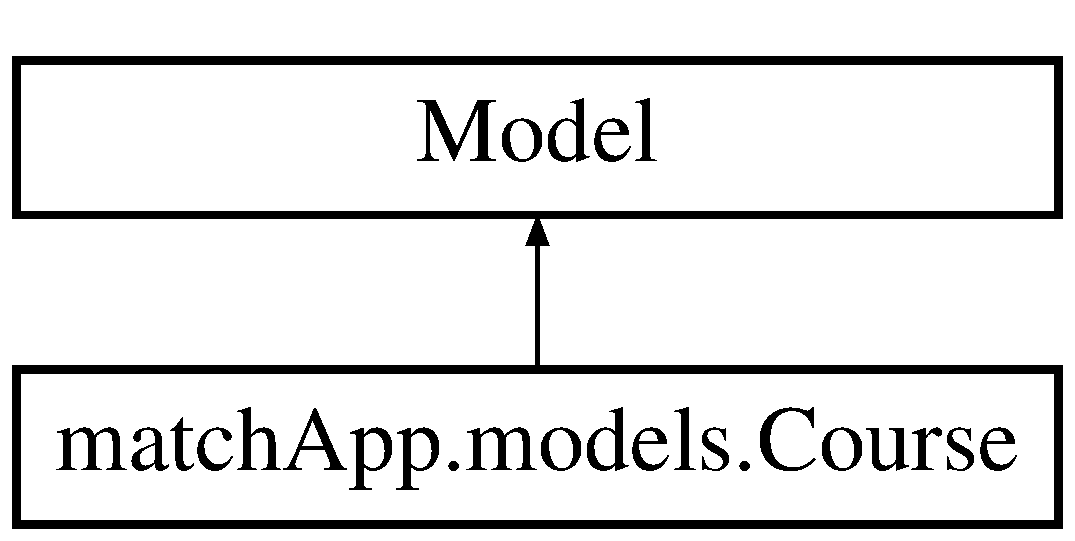
\includegraphics[height=2.000000cm]{classmatch_app_1_1models_1_1_course}
\end{center}
\end{figure}
\subsection*{Public Member Functions}
\begin{DoxyCompactItemize}
\item 
def \hyperlink{classmatch_app_1_1models_1_1_course_aed7d28389b26083cad867c517a9bd291}{\+\_\+\+\_\+unicode\+\_\+\+\_\+} (self)
\end{DoxyCompactItemize}
\subsection*{Static Public Attributes}
\begin{DoxyCompactItemize}
\item 
tuple \hyperlink{classmatch_app_1_1models_1_1_course_afaa80992df56f2f15372c2c523b081c5}{title} = models.\+Char\+Field(max\+\_\+length=64, default=\char`\"{}\char`\"{})
\item 
tuple \hyperlink{classmatch_app_1_1models_1_1_course_a1ed41be5dd960488ff6fe01eb27074f0}{dept\+\_\+id} = models.\+Char\+Field(max\+\_\+length=4, default=\char`\"{}\char`\"{})
\item 
tuple \hyperlink{classmatch_app_1_1models_1_1_course_a1362cefc0918c4ac31f33c4f76197336}{course\+\_\+number} = models.\+Integer\+Field(default=0)
\item 
tuple \hyperlink{classmatch_app_1_1models_1_1_course_a168a91e7508091bc0e34384242946d4e}{catalog\+\_\+page} = models.\+U\+R\+L\+Field(default=\char`\"{}http\+://www.\+colorado.\+edu/catalog/2015-\/16/courses\char`\"{})
\end{DoxyCompactItemize}


\subsection{Detailed Description}
\begin{DoxyVerb}Named course, but essentially creates a class for the classes available on platypus.
Attributes: 
title -- name of course 
dept_id -- department prefix, example CSCI 
course_number -- example 1300 for CSCI 1300 
catalog_page --  link to the page where the course is located in the CU course catalog
\end{DoxyVerb}
 

\subsection{Member Function Documentation}
\hypertarget{classmatch_app_1_1models_1_1_course_aed7d28389b26083cad867c517a9bd291}{}\index{match\+App\+::models\+::\+Course@{match\+App\+::models\+::\+Course}!\+\_\+\+\_\+unicode\+\_\+\+\_\+@{\+\_\+\+\_\+unicode\+\_\+\+\_\+}}
\index{\+\_\+\+\_\+unicode\+\_\+\+\_\+@{\+\_\+\+\_\+unicode\+\_\+\+\_\+}!match\+App\+::models\+::\+Course@{match\+App\+::models\+::\+Course}}
\subsubsection[{\+\_\+\+\_\+unicode\+\_\+\+\_\+}]{\setlength{\rightskip}{0pt plus 5cm}def match\+App.\+models.\+Course.\+\_\+\+\_\+unicode\+\_\+\+\_\+ (
\begin{DoxyParamCaption}
\item[{}]{self}
\end{DoxyParamCaption}
)}\label{classmatch_app_1_1models_1_1_course_aed7d28389b26083cad867c517a9bd291}


\subsection{Member Data Documentation}
\hypertarget{classmatch_app_1_1models_1_1_course_a168a91e7508091bc0e34384242946d4e}{}\index{match\+App\+::models\+::\+Course@{match\+App\+::models\+::\+Course}!catalog\+\_\+page@{catalog\+\_\+page}}
\index{catalog\+\_\+page@{catalog\+\_\+page}!match\+App\+::models\+::\+Course@{match\+App\+::models\+::\+Course}}
\subsubsection[{catalog\+\_\+page}]{\setlength{\rightskip}{0pt plus 5cm}tuple match\+App.\+models.\+Course.\+catalog\+\_\+page = models.\+U\+R\+L\+Field(default=\char`\"{}http\+://www.\+colorado.\+edu/catalog/2015-\/16/courses\char`\"{})\hspace{0.3cm}{\ttfamily [static]}}\label{classmatch_app_1_1models_1_1_course_a168a91e7508091bc0e34384242946d4e}
\hypertarget{classmatch_app_1_1models_1_1_course_a1362cefc0918c4ac31f33c4f76197336}{}\index{match\+App\+::models\+::\+Course@{match\+App\+::models\+::\+Course}!course\+\_\+number@{course\+\_\+number}}
\index{course\+\_\+number@{course\+\_\+number}!match\+App\+::models\+::\+Course@{match\+App\+::models\+::\+Course}}
\subsubsection[{course\+\_\+number}]{\setlength{\rightskip}{0pt plus 5cm}tuple match\+App.\+models.\+Course.\+course\+\_\+number = models.\+Integer\+Field(default=0)\hspace{0.3cm}{\ttfamily [static]}}\label{classmatch_app_1_1models_1_1_course_a1362cefc0918c4ac31f33c4f76197336}
\hypertarget{classmatch_app_1_1models_1_1_course_a1ed41be5dd960488ff6fe01eb27074f0}{}\index{match\+App\+::models\+::\+Course@{match\+App\+::models\+::\+Course}!dept\+\_\+id@{dept\+\_\+id}}
\index{dept\+\_\+id@{dept\+\_\+id}!match\+App\+::models\+::\+Course@{match\+App\+::models\+::\+Course}}
\subsubsection[{dept\+\_\+id}]{\setlength{\rightskip}{0pt plus 5cm}tuple match\+App.\+models.\+Course.\+dept\+\_\+id = models.\+Char\+Field(max\+\_\+length=4, default=\char`\"{}\char`\"{})\hspace{0.3cm}{\ttfamily [static]}}\label{classmatch_app_1_1models_1_1_course_a1ed41be5dd960488ff6fe01eb27074f0}
\hypertarget{classmatch_app_1_1models_1_1_course_afaa80992df56f2f15372c2c523b081c5}{}\index{match\+App\+::models\+::\+Course@{match\+App\+::models\+::\+Course}!title@{title}}
\index{title@{title}!match\+App\+::models\+::\+Course@{match\+App\+::models\+::\+Course}}
\subsubsection[{title}]{\setlength{\rightskip}{0pt plus 5cm}tuple match\+App.\+models.\+Course.\+title = models.\+Char\+Field(max\+\_\+length=64, default=\char`\"{}\char`\"{})\hspace{0.3cm}{\ttfamily [static]}}\label{classmatch_app_1_1models_1_1_course_afaa80992df56f2f15372c2c523b081c5}


The documentation for this class was generated from the following file\+:\begin{DoxyCompactItemize}
\item 
match\+App/\hyperlink{models_8py}{models.\+py}\end{DoxyCompactItemize}

\section{match\+App.\+forms.\+User\+Form.\+Meta Class Reference}
\label{classmatch_app_1_1forms_1_1_user_form_1_1_meta}\index{match\+App.\+forms.\+User\+Form.\+Meta@{match\+App.\+forms.\+User\+Form.\+Meta}}
\subsection*{Static Public Attributes}
\begin{DoxyCompactItemize}
\item 
{\bf model} = User
\item 
tuple {\bf fields} = (\textquotesingle{}username\textquotesingle{}, \textquotesingle{}first\+\_\+name\textquotesingle{}, \textquotesingle{}last\+\_\+name\textquotesingle{}, \textquotesingle{}email\textquotesingle{}, \textquotesingle{}{\bf password}\textquotesingle{})
\end{DoxyCompactItemize}


\subsection{Detailed Description}
\begin{DoxyVerb}Meta defines model and fields for User\end{DoxyVerb}
 

\subsection{Member Data Documentation}
\index{match\+App\+::forms\+::\+User\+Form\+::\+Meta@{match\+App\+::forms\+::\+User\+Form\+::\+Meta}!fields@{fields}}
\index{fields@{fields}!match\+App\+::forms\+::\+User\+Form\+::\+Meta@{match\+App\+::forms\+::\+User\+Form\+::\+Meta}}
\subsubsection[{fields}]{\setlength{\rightskip}{0pt plus 5cm}tuple match\+App.\+forms.\+User\+Form.\+Meta.\+fields = (\textquotesingle{}username\textquotesingle{}, \textquotesingle{}first\+\_\+name\textquotesingle{}, \textquotesingle{}last\+\_\+name\textquotesingle{}, \textquotesingle{}email\textquotesingle{}, \textquotesingle{}{\bf password}\textquotesingle{})\hspace{0.3cm}{\ttfamily [static]}}\label{classmatch_app_1_1forms_1_1_user_form_1_1_meta_afe2afbc82f901ad4b2f8c4df86bc3216}
\index{match\+App\+::forms\+::\+User\+Form\+::\+Meta@{match\+App\+::forms\+::\+User\+Form\+::\+Meta}!model@{model}}
\index{model@{model}!match\+App\+::forms\+::\+User\+Form\+::\+Meta@{match\+App\+::forms\+::\+User\+Form\+::\+Meta}}
\subsubsection[{model}]{\setlength{\rightskip}{0pt plus 5cm}match\+App.\+forms.\+User\+Form.\+Meta.\+model = User\hspace{0.3cm}{\ttfamily [static]}}\label{classmatch_app_1_1forms_1_1_user_form_1_1_meta_a5d9648ab073e418b0cfa6b4883c32423}


The documentation for this class was generated from the following file\+:\begin{DoxyCompactItemize}
\item 
match\+App/{\bf forms.\+py}\end{DoxyCompactItemize}

\section{match\+App.\+models.\+Section Class Reference}
\label{classmatch_app_1_1models_1_1_section}\index{match\+App.\+models.\+Section@{match\+App.\+models.\+Section}}
Inheritance diagram for match\+App.\+models.\+Section\+:\begin{figure}[H]
\begin{center}
\leavevmode
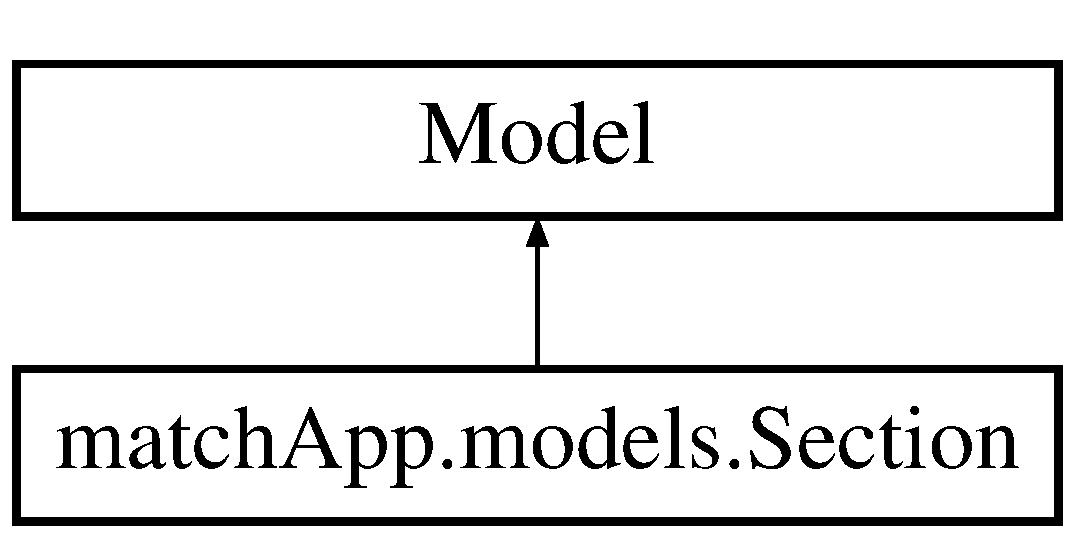
\includegraphics[height=2.000000cm]{classmatch_app_1_1models_1_1_section}
\end{center}
\end{figure}
\subsection*{Public Member Functions}
\begin{DoxyCompactItemize}
\item 
def {\bf \+\_\+\+\_\+unicode\+\_\+\+\_\+} (self)
\end{DoxyCompactItemize}
\subsection*{Static Public Attributes}
\begin{DoxyCompactItemize}
\item 
tuple {\bf class\+\_\+id} = models.\+Integer\+Field(default=0)
\item 
tuple {\bf course\+\_\+title} = models.\+Foreign\+Key({\bf Course}, null=True)
\item 
tuple {\bf section\+\_\+number} = models.\+Integer\+Field(default=0)
\end{DoxyCompactItemize}


\subsection{Detailed Description}
\begin{DoxyVerb}Differentiate between different sections of the same class. 
Attirbutes: 
class_id -- example CSCI 1300
course_title -- name of course, passed as argument for constructor for new section creation
section_number -- unique section number for class section
\end{DoxyVerb}
 

\subsection{Member Function Documentation}
\index{match\+App\+::models\+::\+Section@{match\+App\+::models\+::\+Section}!\+\_\+\+\_\+unicode\+\_\+\+\_\+@{\+\_\+\+\_\+unicode\+\_\+\+\_\+}}
\index{\+\_\+\+\_\+unicode\+\_\+\+\_\+@{\+\_\+\+\_\+unicode\+\_\+\+\_\+}!match\+App\+::models\+::\+Section@{match\+App\+::models\+::\+Section}}
\subsubsection[{\+\_\+\+\_\+unicode\+\_\+\+\_\+}]{\setlength{\rightskip}{0pt plus 5cm}def match\+App.\+models.\+Section.\+\_\+\+\_\+unicode\+\_\+\+\_\+ (
\begin{DoxyParamCaption}
\item[{}]{self}
\end{DoxyParamCaption}
)}\label{classmatch_app_1_1models_1_1_section_a2a520eeadd2c5a65b9cee06f806eee3b}


\subsection{Member Data Documentation}
\index{match\+App\+::models\+::\+Section@{match\+App\+::models\+::\+Section}!class\+\_\+id@{class\+\_\+id}}
\index{class\+\_\+id@{class\+\_\+id}!match\+App\+::models\+::\+Section@{match\+App\+::models\+::\+Section}}
\subsubsection[{class\+\_\+id}]{\setlength{\rightskip}{0pt plus 5cm}tuple match\+App.\+models.\+Section.\+class\+\_\+id = models.\+Integer\+Field(default=0)\hspace{0.3cm}{\ttfamily [static]}}\label{classmatch_app_1_1models_1_1_section_a53207e5dc7ac5210adeb7c4c638689c6}
\index{match\+App\+::models\+::\+Section@{match\+App\+::models\+::\+Section}!course\+\_\+title@{course\+\_\+title}}
\index{course\+\_\+title@{course\+\_\+title}!match\+App\+::models\+::\+Section@{match\+App\+::models\+::\+Section}}
\subsubsection[{course\+\_\+title}]{\setlength{\rightskip}{0pt plus 5cm}tuple match\+App.\+models.\+Section.\+course\+\_\+title = models.\+Foreign\+Key({\bf Course}, null=True)\hspace{0.3cm}{\ttfamily [static]}}\label{classmatch_app_1_1models_1_1_section_a39b73047a0a202fd7da8d54f45690820}
\index{match\+App\+::models\+::\+Section@{match\+App\+::models\+::\+Section}!section\+\_\+number@{section\+\_\+number}}
\index{section\+\_\+number@{section\+\_\+number}!match\+App\+::models\+::\+Section@{match\+App\+::models\+::\+Section}}
\subsubsection[{section\+\_\+number}]{\setlength{\rightskip}{0pt plus 5cm}tuple match\+App.\+models.\+Section.\+section\+\_\+number = models.\+Integer\+Field(default=0)\hspace{0.3cm}{\ttfamily [static]}}\label{classmatch_app_1_1models_1_1_section_ae71939f61c0134b1bc0e02eab1b517d3}


The documentation for this class was generated from the following file\+:\begin{DoxyCompactItemize}
\item 
match\+App/{\bf models.\+py}\end{DoxyCompactItemize}

\hypertarget{classmatch_app_1_1models_1_1_student}{}\section{match\+App.\+models.\+Student Class Reference}
\label{classmatch_app_1_1models_1_1_student}\index{match\+App.\+models.\+Student@{match\+App.\+models.\+Student}}
Inheritance diagram for match\+App.\+models.\+Student\+:\begin{figure}[H]
\begin{center}
\leavevmode
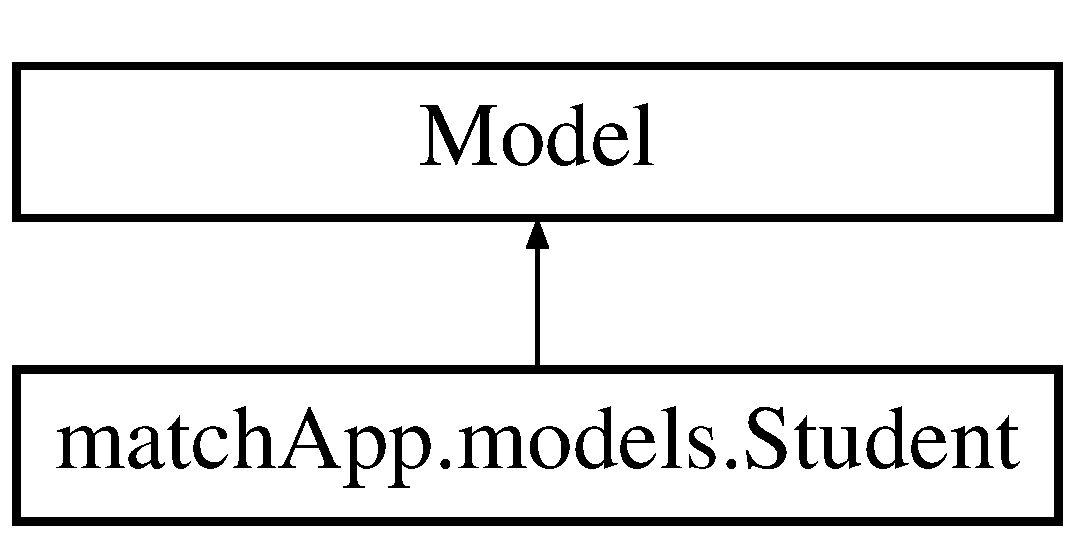
\includegraphics[height=2.000000cm]{classmatch_app_1_1models_1_1_student}
\end{center}
\end{figure}
\subsection*{Public Member Functions}
\begin{DoxyCompactItemize}
\item 
def \hyperlink{classmatch_app_1_1models_1_1_student_a943c2dcc1a40a150c9df5b5741d763a0}{\+\_\+\+\_\+unicode\+\_\+\+\_\+} (self)
\end{DoxyCompactItemize}
\subsection*{Static Public Attributes}
\begin{DoxyCompactItemize}
\item 
tuple \hyperlink{classmatch_app_1_1models_1_1_student_ab99adbde45247ad55b887f0e6360ff9f}{user} = models.\+Foreign\+Key(User)
\item 
tuple \hyperlink{classmatch_app_1_1models_1_1_student_a5df96ebd643f4251fbcd50c2d81a36c0}{course\+\_\+list} = models.\+Char\+Field(max\+\_\+length=1024, default=\char`\"{}\char`\"{})
\end{DoxyCompactItemize}


\subsection{Detailed Description}
\begin{DoxyVerb}Class to handle a user. 
Note: student now returns username, username is assigned to student_id 
Attributes: 
user -- user identity unique to each student
course_list -- list of courses specific to the student/user
\end{DoxyVerb}
 

\subsection{Member Function Documentation}
\hypertarget{classmatch_app_1_1models_1_1_student_a943c2dcc1a40a150c9df5b5741d763a0}{}\index{match\+App\+::models\+::\+Student@{match\+App\+::models\+::\+Student}!\+\_\+\+\_\+unicode\+\_\+\+\_\+@{\+\_\+\+\_\+unicode\+\_\+\+\_\+}}
\index{\+\_\+\+\_\+unicode\+\_\+\+\_\+@{\+\_\+\+\_\+unicode\+\_\+\+\_\+}!match\+App\+::models\+::\+Student@{match\+App\+::models\+::\+Student}}
\subsubsection[{\+\_\+\+\_\+unicode\+\_\+\+\_\+}]{\setlength{\rightskip}{0pt plus 5cm}def match\+App.\+models.\+Student.\+\_\+\+\_\+unicode\+\_\+\+\_\+ (
\begin{DoxyParamCaption}
\item[{}]{self}
\end{DoxyParamCaption}
)}\label{classmatch_app_1_1models_1_1_student_a943c2dcc1a40a150c9df5b5741d763a0}


\subsection{Member Data Documentation}
\hypertarget{classmatch_app_1_1models_1_1_student_a5df96ebd643f4251fbcd50c2d81a36c0}{}\index{match\+App\+::models\+::\+Student@{match\+App\+::models\+::\+Student}!course\+\_\+list@{course\+\_\+list}}
\index{course\+\_\+list@{course\+\_\+list}!match\+App\+::models\+::\+Student@{match\+App\+::models\+::\+Student}}
\subsubsection[{course\+\_\+list}]{\setlength{\rightskip}{0pt plus 5cm}tuple match\+App.\+models.\+Student.\+course\+\_\+list = models.\+Char\+Field(max\+\_\+length=1024, default=\char`\"{}\char`\"{})\hspace{0.3cm}{\ttfamily [static]}}\label{classmatch_app_1_1models_1_1_student_a5df96ebd643f4251fbcd50c2d81a36c0}
\hypertarget{classmatch_app_1_1models_1_1_student_ab99adbde45247ad55b887f0e6360ff9f}{}\index{match\+App\+::models\+::\+Student@{match\+App\+::models\+::\+Student}!user@{user}}
\index{user@{user}!match\+App\+::models\+::\+Student@{match\+App\+::models\+::\+Student}}
\subsubsection[{user}]{\setlength{\rightskip}{0pt plus 5cm}tuple match\+App.\+models.\+Student.\+user = models.\+Foreign\+Key(User)\hspace{0.3cm}{\ttfamily [static]}}\label{classmatch_app_1_1models_1_1_student_ab99adbde45247ad55b887f0e6360ff9f}


The documentation for this class was generated from the following file\+:\begin{DoxyCompactItemize}
\item 
match\+App/\hyperlink{models_8py}{models.\+py}\end{DoxyCompactItemize}

\section{match\+App.\+forms.\+User\+Form Class Reference}
\label{classmatch_app_1_1forms_1_1_user_form}\index{match\+App.\+forms.\+User\+Form@{match\+App.\+forms.\+User\+Form}}
Inheritance diagram for match\+App.\+forms.\+User\+Form\+:\begin{figure}[H]
\begin{center}
\leavevmode
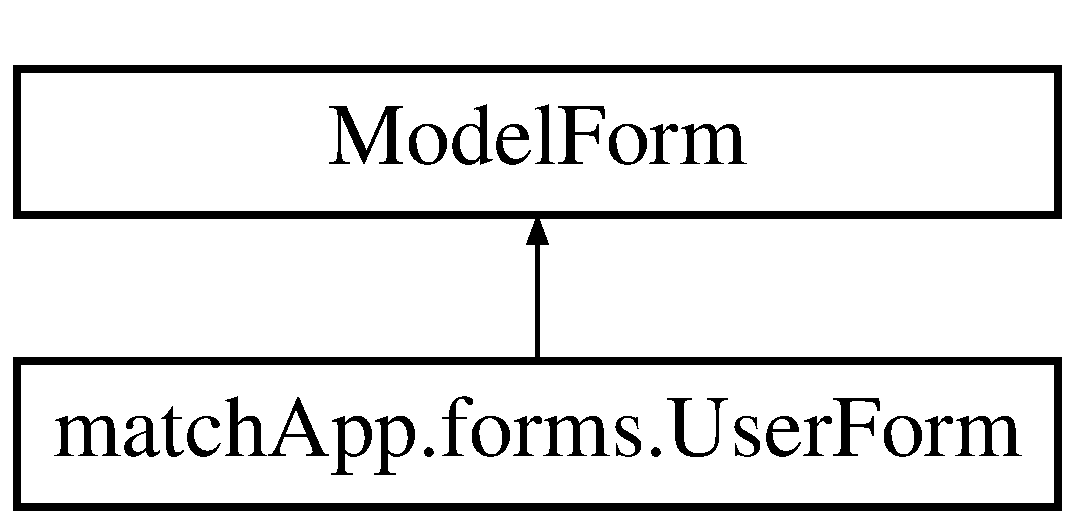
\includegraphics[height=2.000000cm]{classmatch_app_1_1forms_1_1_user_form}
\end{center}
\end{figure}
\subsection*{Classes}
\begin{DoxyCompactItemize}
\item 
class {\bf Meta}
\end{DoxyCompactItemize}
\subsection*{Static Public Attributes}
\begin{DoxyCompactItemize}
\item 
tuple {\bf password} = forms.\+Char\+Field(widget=forms.\+Password\+Input())
\end{DoxyCompactItemize}


\subsection{Member Data Documentation}
\index{match\+App\+::forms\+::\+User\+Form@{match\+App\+::forms\+::\+User\+Form}!password@{password}}
\index{password@{password}!match\+App\+::forms\+::\+User\+Form@{match\+App\+::forms\+::\+User\+Form}}
\subsubsection[{password}]{\setlength{\rightskip}{0pt plus 5cm}tuple match\+App.\+forms.\+User\+Form.\+password = forms.\+Char\+Field(widget=forms.\+Password\+Input())\hspace{0.3cm}{\ttfamily [static]}}\label{classmatch_app_1_1forms_1_1_user_form_a22fba20516b0361b6db1a96fc08c5053}


The documentation for this class was generated from the following file\+:\begin{DoxyCompactItemize}
\item 
match\+App/{\bf forms.\+py}\end{DoxyCompactItemize}

\chapter{File Documentation}
\hypertarget{manage_8py}{}\section{manage.\+py File Reference}
\label{manage_8py}\index{manage.\+py@{manage.\+py}}
\subsection*{Namespaces}
\begin{DoxyCompactItemize}
\item 
 \hyperlink{namespacemanage}{manage}
\end{DoxyCompactItemize}

\hypertarget{match_app_2____init_____8py}{}\section{match\+App/\+\_\+\+\_\+init\+\_\+\+\_\+.py File Reference}
\label{match_app_2____init_____8py}\index{match\+App/\+\_\+\+\_\+init\+\_\+\+\_\+.\+py@{match\+App/\+\_\+\+\_\+init\+\_\+\+\_\+.\+py}}
\subsection*{Namespaces}
\begin{DoxyCompactItemize}
\item 
 \hyperlink{namespacematch_app}{match\+App}
\end{DoxyCompactItemize}

\hypertarget{match_app_2matching_algorithm_2____init_____8py}{}\section{match\+App/matching\+Algorithm/\+\_\+\+\_\+init\+\_\+\+\_\+.py File Reference}
\label{match_app_2matching_algorithm_2____init_____8py}\index{match\+App/matching\+Algorithm/\+\_\+\+\_\+init\+\_\+\+\_\+.\+py@{match\+App/matching\+Algorithm/\+\_\+\+\_\+init\+\_\+\+\_\+.\+py}}
\subsection*{Namespaces}
\begin{DoxyCompactItemize}
\item 
 \hyperlink{namespacematch_app_1_1matching_algorithm}{match\+App.\+matching\+Algorithm}
\end{DoxyCompactItemize}

\section{match\+App/templatetags/\+\_\+\+\_\+init\+\_\+\+\_\+.py File Reference}
\label{match_app_2templatetags_2____init_____8py}\index{match\+App/templatetags/\+\_\+\+\_\+init\+\_\+\+\_\+.\+py@{match\+App/templatetags/\+\_\+\+\_\+init\+\_\+\+\_\+.\+py}}
\subsection*{Namespaces}
\begin{DoxyCompactItemize}
\item 
 {\bf match\+App.\+templatetags}
\end{DoxyCompactItemize}

\hypertarget{_platypus_2____init_____8py}{}\section{Platypus/\+\_\+\+\_\+init\+\_\+\+\_\+.py File Reference}
\label{_platypus_2____init_____8py}\index{Platypus/\+\_\+\+\_\+init\+\_\+\+\_\+.\+py@{Platypus/\+\_\+\+\_\+init\+\_\+\+\_\+.\+py}}
\subsection*{Namespaces}
\begin{DoxyCompactItemize}
\item 
 \hyperlink{namespace_platypus}{Platypus}
\end{DoxyCompactItemize}

\hypertarget{admin_8py}{}\section{match\+App/admin.py File Reference}
\label{admin_8py}\index{match\+App/admin.\+py@{match\+App/admin.\+py}}
\subsection*{Namespaces}
\begin{DoxyCompactItemize}
\item 
 \hyperlink{namespacematch_app_1_1admin}{match\+App.\+admin}
\end{DoxyCompactItemize}

\hypertarget{forms_8py}{}\section{match\+App/forms.py File Reference}
\label{forms_8py}\index{match\+App/forms.\+py@{match\+App/forms.\+py}}
\subsection*{Classes}
\begin{DoxyCompactItemize}
\item 
class \hyperlink{classmatch_app_1_1forms_1_1_user_form}{match\+App.\+forms.\+User\+Form}
\item 
class \hyperlink{classmatch_app_1_1forms_1_1_user_form_1_1_meta}{match\+App.\+forms.\+User\+Form.\+Meta}
\end{DoxyCompactItemize}
\subsection*{Namespaces}
\begin{DoxyCompactItemize}
\item 
 \hyperlink{namespacematch_app_1_1forms}{match\+App.\+forms}
\end{DoxyCompactItemize}

\section{match\+App/html/dynsections.js File Reference}
\label{dynsections_8js}\index{match\+App/html/dynsections.\+js@{match\+App/html/dynsections.\+js}}
\subsection*{Functions}
\begin{DoxyCompactItemize}
\item 
function {\bf toggle\+Visibility} (link\+Obj)
\item 
function {\bf update\+Stripes} ()
\item 
function {\bf toggle\+Level} (level)
\item 
function {\bf toggle\+Folder} (id)
\item 
function {\bf toggle\+Inherit} (id)
\end{DoxyCompactItemize}


\subsection{Function Documentation}
\index{dynsections.\+js@{dynsections.\+js}!toggle\+Folder@{toggle\+Folder}}
\index{toggle\+Folder@{toggle\+Folder}!dynsections.\+js@{dynsections.\+js}}
\subsubsection[{toggle\+Folder}]{\setlength{\rightskip}{0pt plus 5cm}function toggle\+Folder (
\begin{DoxyParamCaption}
\item[{}]{id}
\end{DoxyParamCaption}
)}\label{dynsections_8js_af244da4527af2d845dca04f5656376cd}
\index{dynsections.\+js@{dynsections.\+js}!toggle\+Inherit@{toggle\+Inherit}}
\index{toggle\+Inherit@{toggle\+Inherit}!dynsections.\+js@{dynsections.\+js}}
\subsubsection[{toggle\+Inherit}]{\setlength{\rightskip}{0pt plus 5cm}function toggle\+Inherit (
\begin{DoxyParamCaption}
\item[{}]{id}
\end{DoxyParamCaption}
)}\label{dynsections_8js_ac057b640b17ff32af11ced151c9305b4}
\index{dynsections.\+js@{dynsections.\+js}!toggle\+Level@{toggle\+Level}}
\index{toggle\+Level@{toggle\+Level}!dynsections.\+js@{dynsections.\+js}}
\subsubsection[{toggle\+Level}]{\setlength{\rightskip}{0pt plus 5cm}function toggle\+Level (
\begin{DoxyParamCaption}
\item[{}]{level}
\end{DoxyParamCaption}
)}\label{dynsections_8js_a19f577cc1ba571396a85bb1f48bf4df2}
\index{dynsections.\+js@{dynsections.\+js}!toggle\+Visibility@{toggle\+Visibility}}
\index{toggle\+Visibility@{toggle\+Visibility}!dynsections.\+js@{dynsections.\+js}}
\subsubsection[{toggle\+Visibility}]{\setlength{\rightskip}{0pt plus 5cm}function toggle\+Visibility (
\begin{DoxyParamCaption}
\item[{}]{link\+Obj}
\end{DoxyParamCaption}
)}\label{dynsections_8js_a1922c462474df7dfd18741c961d59a25}
\index{dynsections.\+js@{dynsections.\+js}!update\+Stripes@{update\+Stripes}}
\index{update\+Stripes@{update\+Stripes}!dynsections.\+js@{dynsections.\+js}}
\subsubsection[{update\+Stripes}]{\setlength{\rightskip}{0pt plus 5cm}function update\+Stripes (
\begin{DoxyParamCaption}
{}
\end{DoxyParamCaption}
)}\label{dynsections_8js_a8f7493ad859d4fbf2523917511ee7177}

\section{match\+App/html/jquery.js File Reference}
\label{jquery_8js}\index{match\+App/html/jquery.\+js@{match\+App/html/jquery.\+js}}
\subsection*{Functions}
\begin{DoxyCompactItemize}
\item 
{\bf b} {\bf extend} (\{css\+Hooks\+:\{opacity\+:\{get\+:function(bw, bv)\{{\bf if}(bv)\{var {\bf e}={\bf Z}(bw,\char`\"{}opacity\char`\"{},\char`\"{}opacity\char`\"{});return {\bf e}===\char`\"{}\char`\"{}?\char`\"{}1\char`\"{}\+:{\bf e}\}else\{return bw.\+style.\+opacity\}\}\}\}, css\+Number\+:\{fill\+Opacity\+:true, font\+Weight\+:true, line\+Height\+:true, opacity\+:true, orphans\+:true, widows\+:true, z\+Index\+:true, zoom\+:true\}, css\+Props\+:\{\char`\"{}float\char`\"{}\+:b.\+support.\+css\+Float?\char`\"{}css\+Float\char`\"{}\+:\char`\"{}style\+Float\char`\"{}\}, style\+:function(bx, bw, b\+D, by)\{{\bf if}(!bx$\vert$$\vert$bx.\+node\+Type===3$\vert$$\vert$bx.\+node\+Type===8$\vert$$\vert$!bx.\+style)\{return\}var b\+B, b\+C, bz=b.\+camel\+Case(bw), bv=bx.\+style, b\+E=b.\+css\+Hooks[bz];bw=b.\+css\+Props[bz]$\vert$$\vert$bz;{\bf if}(b\+D!=={\bf L})\{b\+C=typeof b\+D;{\bf if}(b\+C===\char`\"{}string\char`\"{}\&\&(b\+B=I.\+exec(b\+D)))\{b\+D=(+(b\+B[1]+1)$\ast$+b\+B[2])+parse\+Float({\bf b.\+css}(bx, bw));b\+C=\char`\"{}number\char`\"{}\}if(b\+D==null$\vert$$\vert$b\+C===\char`\"{}number\char`\"{}\&\&is\+Na\+N(b\+D))\{return\}{\bf if}(b\+C===\char`\"{}number\char`\"{}\&\&!b.\+css\+Number[bz])\{b\+D+=\char`\"{}px\char`\"{}\}if(!b\+E$\vert$$\vert$!(\char`\"{}set\char`\"{}in b\+E)$\vert$$\vert$(b\+D=b\+E.\+set(bx, b\+D))!=={\bf L})\{try\{bv[bw]=b\+D\}catch(b\+A)\{\}\}\}else\{{\bf if}(b\+E \&\&\char`\"{}get\char`\"{}in b\+E \&\&(b\+B=b\+E.\+get(bx, false, by))!=={\bf L})\{return b\+B\}return bv[bw]\}\}, css\+:function(by, bx, bv)\{var bw, {\bf e};bx=b.\+camel\+Case(bx);{\bf e}=b.\+css\+Hooks[bx];bx=b.\+css\+Props[bx]$\vert$$\vert$bx;{\bf if}(bx===\char`\"{}css\+Float\char`\"{})\{bx=\char`\"{}float\char`\"{}\}if({\bf e} \&\&\char`\"{}get\char`\"{}in {\bf e} \&\&(bw=e.\+get(by, true, bv))!=={\bf L})\{return bw\}else\{{\bf if}({\bf Z})\{return {\bf Z}(by, bx)\}\}\}, swap\+:function(bx, bw, by)\{var {\bf e}=\{\};for(var bv in bw)\{{\bf e}[bv]=bx.\+style[bv];bx.\+style[bv]=bw[bv]\}by.\+call(bx);for(bv in bw)\{bx.\+style[bv]={\bf e}[bv]\}\}\})
\item 
{\bf b} {\bf each} ([\char`\"{}height\char`\"{},\char`\"{}width\char`\"{}], function(bv, {\bf e})\{b.\+css\+Hooks[{\bf e}]=\{get\+:function(by, bx, bw)\{var bz;{\bf if}(bx)\{{\bf if}(by.\+offset\+Width!==0)\{return {\bf p}(by, {\bf e}, bw)\}else\{b.\+swap(by, a7, function()\{bz={\bf p}(by, {\bf e}, bw)\})\}return bz\}\}, set\+:function(bw, bx)\{{\bf if}(bc.\+test(bx))\{bx=parse\+Float(bx);{\bf if}(bx $>$=0)\{return bx+\char`\"{}px\char`\"{}\}\}else\{return bx\}\}\}\})
\item 
{\bf if} (!b.\+support.\+opacity)
\item 
{\bf b} (function()\{{\bf if}(!b.\+support.\+reliable\+Margin\+Right)\{b.\+css\+Hooks.\+margin\+Right=\{get\+:function(bw, bv)\{var {\bf e};b.\+swap(bw,\{display\+:\char`\"{}inline-\/block\char`\"{}\}, function()\{{\bf if}(bv)\{{\bf e}={\bf Z}(bw,\char`\"{}margin-\/right\char`\"{},\char`\"{}margin\+Right\char`\"{})\}else\{{\bf e}=bw.\+style.\+margin\+Right\}\});return {\bf e}\}\}\}\})
\item 
{\bf if} (av.\+default\+View \&\&av.\+default\+View.\+get\+Computed\+Style)
\item 
{\bf if} (av.\+document\+Element.\+current\+Style)
\item 
function {\bf p} (by, bw, bv)
\item 
{\bf if} (b.\+expr \&\&b.\+expr.\+filters)
\end{DoxyCompactItemize}
\subsection*{Variables}
\begin{DoxyCompactItemize}
\item 
function {\bf bb}
\item 
function {\bf L} \{var av=bb.\+document,bu=bb.\+navigator,bl=bb.\+location
\item 
var {\bf b}
\item 
var {\bf au} =/opacity=([$^\wedge$)]$\ast$)/,z=/([A-\/{\bf Z}]$\vert$$^\wedge$ms)/g,bc=/$^\wedge$-\/?\textbackslash{}{\bf d}+(?\+:px)?\$/i,bn=/$^\wedge$-\/?\textbackslash{}{\bf d}/,I=/$^\wedge$([\textbackslash{}-\/+])=([\textbackslash{}-\/+.\textbackslash{}de]+)/,a7=\{position\+:\char`\"{}absolute\char`\"{},visibility\+:\char`\"{}hidden\char`\"{},display\+:\char`\"{}block\char`\"{}\},an=[\char`\"{}Left\char`\"{},\char`\"{}Right\char`\"{}],a1=[\char`\"{}Top\char`\"{},\char`\"{}Bottom\char`\"{}],Z,a\+I,a\+X
\item 
{\bf b} fn {\bf css} =function({\bf e},bv)\{{\bf if}(arguments.\+length===2\&\&bv==={\bf L})\{return this\}return b.\+access(this,{\bf e},bv,true,function(bx,bw,by)\{return by!=={\bf L}?b.\+style(bx,bw,by)\+:b.\+css(bx,bw)\})\}
\item 
{\bf b} {\bf cur\+C\+S\+S} ={\bf b.\+css}
\item 
{\bf Z} =a\+I$\vert$$\vert$a\+X
\item 
var {\bf k} =/\%20/g
\item 
var {\bf ap} =/\textbackslash{}[\textbackslash{}]\$/
\item 
var {\bf bs} =/\textbackslash{}r?\textbackslash{}n/g
\item 
var {\bf bq} =/\#.$\ast$\$/
\item 
var {\bf a\+D} =/$^\wedge$(.$\ast$?)\+:[ \textbackslash{}t]$\ast$([$^\wedge$\textbackslash{}r\textbackslash{}n]$\ast$)\textbackslash{}r?\$/mg
\item 
var {\bf a\+Z} =/$^\wedge$(?\+:color$\vert$date$\vert$datetime$\vert$datetime-\/local$\vert$email$\vert$hidden$\vert$month$\vert$number$\vert$password$\vert$range$\vert$search$\vert$tel$\vert$text$\vert$time$\vert$url$\vert$week)\$/i
\item 
var {\bf a\+M} =/$^\wedge$(?\+:about$\vert$app$\vert$app\textbackslash{}-\/storage$\vert$.+\textbackslash{}-\/extension$\vert$file$\vert$res$\vert$widget)\+:\$/
\item 
var {\bf a\+Q} =/$^\wedge$(?\+:G\+E\+T$\vert$H\+E\+A\+D)\$/
\item 
var {\bf c}
\end{DoxyCompactItemize}


\subsection{Function Documentation}
\index{jquery.\+js@{jquery.\+js}!b@{b}}
\index{b@{b}!jquery.\+js@{jquery.\+js}}
\subsubsection[{b}]{\setlength{\rightskip}{0pt plus 5cm}b (
\begin{DoxyParamCaption}
\item[{function()\{{\bf if}(!b.\+support.\+reliable\+Margin\+Right)\{b.\+css\+Hooks.\+margin\+Right=\{get\+:function(bw, bv)\{var {\bf e};b.\+swap(bw,\{display\+:\char`\"{}inline-\/block\char`\"{}\}, function()\{{\bf if}(bv)\{{\bf e}={\bf Z}(bw,\char`\"{}margin-\/right\char`\"{},\char`\"{}margin\+Right\char`\"{})\}else\{{\bf e}=bw.\+style.\+margin\+Right\}\});return {\bf e}\}\}\}\}}]{}
\end{DoxyParamCaption}
)}\label{jquery_8js_a2fa551895933fae935a0a6b87282241d}
\index{jquery.\+js@{jquery.\+js}!each@{each}}
\index{each@{each}!jquery.\+js@{jquery.\+js}}
\subsubsection[{each}]{\setlength{\rightskip}{0pt plus 5cm}{\bf b} each (
\begin{DoxyParamCaption}
\item[{function(bv, {\bf e})\{b.\+css\+Hooks[{\bf e}]=\{get\+:function(by, bx, bw)\{var bz;{\bf if}(bx)\{{\bf if}(by.\+offset\+Width!==0)\{return {\bf p}(by, {\bf e}, bw)\}else\{b.\+swap(by, a7, function()\{bz={\bf p}(by, {\bf e}, bw)\})\}return bz\}\}, set\+:function(bw, bx)\{{\bf if}(bc.\+test(bx))\{bx=parse\+Float(bx);{\bf if}(bx $>$=0)\{return bx+\char`\"{}px\char`\"{}\}\}else\{return bx\}\}\}\}}]{}
\end{DoxyParamCaption}
)}\label{jquery_8js_a871ff39db627c54c710a3e9909b8234c}
\index{jquery.\+js@{jquery.\+js}!extend@{extend}}
\index{extend@{extend}!jquery.\+js@{jquery.\+js}}
\subsubsection[{extend}]{\setlength{\rightskip}{0pt plus 5cm}{\bf b} extend (
\begin{DoxyParamCaption}
\item[{\{css\+Hooks\+:\{opacity\+:\{get\+:function(bw, bv)\{{\bf if}(bv)\{var {\bf e}={\bf Z}(bw,\char`\"{}opacity\char`\"{},\char`\"{}opacity\char`\"{});return {\bf e}===\char`\"{}\char`\"{}?\char`\"{}1\char`\"{}\+:{\bf e}\}else\{return bw.\+style.\+opacity\}\}\}\}, css\+Number\+:\{fill\+Opacity\+:true, font\+Weight\+:true, line\+Height\+:true, opacity\+:true, orphans\+:true, widows\+:true, z\+Index\+:true, zoom\+:true\}, css\+Props\+:\{\char`\"{}float\char`\"{}\+:b.\+support.\+css\+Float?\char`\"{}css\+Float\char`\"{}\+:\char`\"{}style\+Float\char`\"{}\}, style\+:function(bx, bw, b\+D, by)\{{\bf if}(!bx$\vert$$\vert$bx.\+node\+Type===3$\vert$$\vert$bx.\+node\+Type===8$\vert$$\vert$!bx.\+style)\{return\}var b\+B, b\+C, bz=b.\+camel\+Case(bw), bv=bx.\+style, b\+E=b.\+css\+Hooks[bz];bw=b.\+css\+Props[bz]$\vert$$\vert$bz;{\bf if}(b\+D!=={\bf L})\{b\+C=typeof b\+D;{\bf if}(b\+C===\char`\"{}string\char`\"{}\&\&(b\+B=I.\+exec(b\+D)))\{b\+D=(+(b\+B[1]+1)$\ast$+b\+B[2])+parse\+Float({\bf b.\+css}(bx, bw));b\+C=\char`\"{}number\char`\"{}\}if(b\+D==null$\vert$$\vert$b\+C===\char`\"{}number\char`\"{}\&\&is\+Na\+N(b\+D))\{return\}{\bf if}(b\+C===\char`\"{}number\char`\"{}\&\&!b.\+css\+Number[bz])\{b\+D+=\char`\"{}px\char`\"{}\}if(!b\+E$\vert$$\vert$!(\char`\"{}set\char`\"{}in b\+E)$\vert$$\vert$(b\+D=b\+E.\+set(bx, b\+D))!=={\bf L})\{try\{bv[bw]=b\+D\}catch(b\+A)\{\}\}\}else\{{\bf if}(b\+E \&\&\char`\"{}get\char`\"{}in b\+E \&\&(b\+B=b\+E.\+get(bx, false, by))!=={\bf L})\{return b\+B\}return bv[bw]\}\}, css\+:function(by, bx, bv)\{var bw, {\bf e};bx=b.\+camel\+Case(bx);{\bf e}=b.\+css\+Hooks[bx];bx=b.\+css\+Props[bx]$\vert$$\vert$bx;{\bf if}(bx===\char`\"{}css\+Float\char`\"{})\{bx=\char`\"{}float\char`\"{}\}if({\bf e} \&\&\char`\"{}get\char`\"{}in {\bf e} \&\&(bw=e.\+get(by, true, bv))!=={\bf L})\{return bw\}else\{{\bf if}({\bf Z})\{return {\bf Z}(by, bx)\}\}\}, swap\+:function(bx, bw, by)\{var {\bf e}=\{\};for(var bv in bw)\{{\bf e}[bv]=bx.\+style[bv];bx.\+style[bv]=bw[bv]\}by.\+call(bx);for(bv in bw)\{bx.\+style[bv]={\bf e}[bv]\}\}\}}]{}
\end{DoxyParamCaption}
)}\label{jquery_8js_a5fb206c91c64d1be35fde236706eab86}
\index{jquery.\+js@{jquery.\+js}!if@{if}}
\index{if@{if}!jquery.\+js@{jquery.\+js}}
\subsubsection[{if}]{\setlength{\rightskip}{0pt plus 5cm}if (
\begin{DoxyParamCaption}
\item[{av.\+document\+Element.}]{current\+Style}
\end{DoxyParamCaption}
)}\label{jquery_8js_a2c54bd8ed7482e89d19331ba61fe221c}
\index{jquery.\+js@{jquery.\+js}!if@{if}}
\index{if@{if}!jquery.\+js@{jquery.\+js}}
\subsubsection[{if}]{\setlength{\rightskip}{0pt plus 5cm}if (
\begin{DoxyParamCaption}
\item[{av.\+default\+View \&\&av.\+default\+View.}]{get\+Computed\+Style}
\end{DoxyParamCaption}
)}\label{jquery_8js_a30d3d2cd5b567c9f31b2aa30b9cb3bb8}
\index{jquery.\+js@{jquery.\+js}!if@{if}}
\index{if@{if}!jquery.\+js@{jquery.\+js}}
\subsubsection[{if}]{\setlength{\rightskip}{0pt plus 5cm}if (
\begin{DoxyParamCaption}
\item[{b.\+expr \&\&b.\+expr.}]{filters}
\end{DoxyParamCaption}
)}\label{jquery_8js_a42cbfadee2b4749e8f699ea8d745a0e4}
\index{jquery.\+js@{jquery.\+js}!if@{if}}
\index{if@{if}!jquery.\+js@{jquery.\+js}}
\subsubsection[{if}]{\setlength{\rightskip}{0pt plus 5cm}if (
\begin{DoxyParamCaption}
\item[{!b.\+support.}]{opacity}
\end{DoxyParamCaption}
)}\label{jquery_8js_a9db6d45a025ad692282fe23e69eeba43}
\index{jquery.\+js@{jquery.\+js}!p@{p}}
\index{p@{p}!jquery.\+js@{jquery.\+js}}
\subsubsection[{p}]{\setlength{\rightskip}{0pt plus 5cm}function p (
\begin{DoxyParamCaption}
\item[{}]{by, }
\item[{}]{bw, }
\item[{}]{bv}
\end{DoxyParamCaption}
)}\label{jquery_8js_a2335e57f79b6acfb6de59c235dc8a83e}


\subsection{Variable Documentation}
\index{jquery.\+js@{jquery.\+js}!a\+D@{a\+D}}
\index{a\+D@{a\+D}!jquery.\+js@{jquery.\+js}}
\subsubsection[{a\+D}]{\setlength{\rightskip}{0pt plus 5cm}var a\+D =/$^\wedge$(.$\ast$?)\+:[ \textbackslash{}t]$\ast$([$^\wedge$\textbackslash{}r\textbackslash{}n]$\ast$)\textbackslash{}r?\$/mg}\label{jquery_8js_ad223f5fba68c41c1236671ac5c5b0fcb}
\index{jquery.\+js@{jquery.\+js}!a\+M@{a\+M}}
\index{a\+M@{a\+M}!jquery.\+js@{jquery.\+js}}
\subsubsection[{a\+M}]{\setlength{\rightskip}{0pt plus 5cm}var a\+M =/$^\wedge$(?\+:about$\vert$app$\vert$app\textbackslash{}-\/storage$\vert$.+\textbackslash{}-\/extension$\vert$file$\vert$res$\vert$widget)\+:\$/}\label{jquery_8js_a8cc6111a5def3ea889157d13fb9a9672}
\index{jquery.\+js@{jquery.\+js}!ap@{ap}}
\index{ap@{ap}!jquery.\+js@{jquery.\+js}}
\subsubsection[{ap}]{\setlength{\rightskip}{0pt plus 5cm}var ap =/\textbackslash{}[\textbackslash{}]\$/}\label{jquery_8js_a6ddf393cc7f9a8828e197bb0d9916c44}
\index{jquery.\+js@{jquery.\+js}!a\+Q@{a\+Q}}
\index{a\+Q@{a\+Q}!jquery.\+js@{jquery.\+js}}
\subsubsection[{a\+Q}]{\setlength{\rightskip}{0pt plus 5cm}var a\+Q =/$^\wedge$(?\+:G\+E\+T$\vert$H\+E\+A\+D)\$/}\label{jquery_8js_a79eb58dc6cdf0aef563d5dc1ded27df5}
\index{jquery.\+js@{jquery.\+js}!au@{au}}
\index{au@{au}!jquery.\+js@{jquery.\+js}}
\subsubsection[{au}]{\setlength{\rightskip}{0pt plus 5cm}var au =/opacity=([$^\wedge$)]$\ast$)/,z=/([A-\/{\bf Z}]$\vert$$^\wedge$ms)/g,bc=/$^\wedge$-\/?\textbackslash{}{\bf d}+(?\+:px)?\$/i,bn=/$^\wedge$-\/?\textbackslash{}{\bf d}/,I=/$^\wedge$([\textbackslash{}-\/+])=([\textbackslash{}-\/+.\textbackslash{}de]+)/,a7=\{position\+:\char`\"{}absolute\char`\"{},visibility\+:\char`\"{}hidden\char`\"{},display\+:\char`\"{}block\char`\"{}\},an=[\char`\"{}Left\char`\"{},\char`\"{}Right\char`\"{}],a1=[\char`\"{}Top\char`\"{},\char`\"{}Bottom\char`\"{}],Z,a\+I,a\+X}\label{jquery_8js_a4fd8ddfab07c8d7c7cae0ab0e052cad3}
\index{jquery.\+js@{jquery.\+js}!a\+Z@{a\+Z}}
\index{a\+Z@{a\+Z}!jquery.\+js@{jquery.\+js}}
\subsubsection[{a\+Z}]{\setlength{\rightskip}{0pt plus 5cm}var a\+Z =/$^\wedge$(?\+:color$\vert$date$\vert$datetime$\vert$datetime-\/local$\vert$email$\vert$hidden$\vert$month$\vert$number$\vert$password$\vert$range$\vert$search$\vert$tel$\vert$text$\vert$time$\vert$url$\vert$week)\$/i}\label{jquery_8js_ac87125cdee1a5e57da4ef619af49bc7d}
\index{jquery.\+js@{jquery.\+js}!b@{b}}
\index{b@{b}!jquery.\+js@{jquery.\+js}}
\subsubsection[{b}]{\setlength{\rightskip}{0pt plus 5cm}function b}\label{jquery_8js_ac0431efac4d7c393d1e70b86115cb93f}
{\bfseries Initial value\+:}
\begin{DoxyCode}
=(\textcolor{keyword}{function}()\{var bF=\textcolor{keyword}{function}(b0,b1)\{\textcolor{keywordflow}{return} \textcolor{keyword}{new} bF.fn.init(b0,b1,bD)\},bU=bb.jQuery,bH=
      bb.$,bD,bY=/^(?:[^#<]*(<[\(\backslash\)w\(\backslash\)W]+>)[^>]*$|#([\(\backslash\)w\(\backslash\)-]*)$)/,bM=/\(\backslash\)S/,bI=/^\(\backslash\)s+/,bE=/\(\backslash\)s+$/,bA=/^<(\(\backslash\)w+)\(\backslash\)s*\(\backslash\)/?>(?:<\(\backslash\)/\(\backslash\)
      1>)?$/,bN=/^[\(\backslash\)],:\{\}\(\backslash\)s]*$/,bW=/\(\backslash\)\(\backslash\)(?:[\textcolor{stringliteral}{"\(\backslash\)\(\backslash\)\(\backslash\)/bfnrt]|u[0-9a-fA-F]\{4\})/g,bP=/"}[^\textcolor{stringliteral}{"\(\backslash\)\(\backslash\)\(\backslash\)n\(\backslash\)r]*"}|\textcolor{keyword}{true}|\textcolor{keyword}{false}|null|-?
      \d+(?:\(\backslash\).\(\backslash\)d*)?(?:[eE][+\(\backslash\)-]?\(\backslash\)d+)?/g,bJ=/(?:^|:|,)(?:\(\backslash\)s*\(\backslash\)[)+/g,by=/(webkit)[ \(\backslash\)/]([\(\backslash\)w.]+)/,bR=/(opera)(?:.*
      version)?[ \(\backslash\)/]([\(\backslash\)w.]+)/,bQ=/(msie) ([\(\backslash\)w.]+)/,bS=/(mozilla)(?:.*? rv:([\(\backslash\)w.]+))?/,bB=/-([
      a-z]|[0-9])/ig,bZ=/^-ms-/,bT=\textcolor{keyword}{function}(b0,b1)\{\textcolor{keywordflow}{return}(b1+\textcolor{stringliteral}{""}).toUpperCase()\},bX=bu.userAgent,bV,bC,
      e,bL=Object.prototype.toString,bG=Object.prototype.hasOwnProperty,bz=Array.prototype.push,bK=Array.
      prototype.slice,bO=String.prototype.trim,bv=Array.prototype.indexOf,bx=\{\};bF.fn=bF.prototype=\{constructor:bF,init:\textcolor{keyword}{
      function}(b0,b4,b3)\{var b2,b5,b1,b6;\textcolor{keywordflow}{if}(!b0)\{\textcolor{keywordflow}{return} \textcolor{keyword}{this}\}\textcolor{keywordflow}{if}(b0.nodeType)\{this.context=\textcolor{keyword}{this}[0]=b0;this.length=1;\textcolor{keywordflow}{
      return} \textcolor{keyword}{this}\}\textcolor{keywordflow}{if}(b0===\textcolor{stringliteral}{"body"}&&!b4&&av.body)\{this.context=av;\textcolor{keyword}{this}[0]=av.body;this.selector=b0;this.length=1;\textcolor{keywordflow}{
      return} \textcolor{keyword}{this}\}\textcolor{keywordflow}{if}(typeof b0===\textcolor{stringliteral}{"string"})\{\textcolor{keywordflow}{if}(b0.charAt(0)===\textcolor{stringliteral}{"<"}&&b0.charAt(b0.length-1)===\textcolor{stringliteral}{">"}&&b0.length>=3)\{b2=[null
      ,b0,null]\}\textcolor{keywordflow}{else}\{b2=bY.exec(b0)\}\textcolor{keywordflow}{if}(b2&&(b2[1]||!b4))\{\textcolor{keywordflow}{if}(b2[1])\{b4=b4 instanceof bF?b4[0]:b4;b6=(b4?b4.
      ownerDocument||b4:av);b1=bA.exec(b0);\textcolor{keywordflow}{if}(b1)\{\textcolor{keywordflow}{if}(bF.isPlainObject(b4))\{b0=[av.createElement(b1[1])];bF.fn.attr.call(b0
      ,b4,\textcolor{keyword}{true})\}\textcolor{keywordflow}{else}\{b0=[b6.createElement(b1[1])]\}\}\textcolor{keywordflow}{else}\{b1=bF.buildFragment([b2[1]],[b6]);b0=(b1.cacheable?bF.
      clone(b1.fragment):b1.fragment).childNodes\}\textcolor{keywordflow}{return} bF.merge(\textcolor{keyword}{this},b0)\}\textcolor{keywordflow}{else}\{b5=av.getElementById(b2[2]);\textcolor{keywordflow}{if}(b5&&b5.
      parentNode)\{\textcolor{keywordflow}{if}(b5.id!==b2[2])\{\textcolor{keywordflow}{return} b3.find(b0)\}this.length=1;\textcolor{keyword}{this}[0]=b5\}this.context=av;this.selector=b0;\textcolor{keywordflow}{
      return} \textcolor{keyword}{this}\}\}\textcolor{keywordflow}{else}\{\textcolor{keywordflow}{if}(!b4||b4.jquery)\{\textcolor{keywordflow}{return}(b4||b3).find(b0)\}\textcolor{keywordflow}{else}\{\textcolor{keywordflow}{return} this.constructor(b4).find(b0)\}\}\}\textcolor{keywordflow}{else}\{\textcolor{keywordflow}{
      if}(bF.isFunction(b0))\{\textcolor{keywordflow}{return} b3.ready(b0)\}\}\textcolor{keywordflow}{if}(b0.selector!==L)\{this.selector=b0.selector;this.context=b0.
      context\}\textcolor{keywordflow}{return} bF.makeArray(b0,\textcolor{keyword}{this})\},selector:\textcolor{stringliteral}{""},jquery:\textcolor{stringliteral}{"1.7.1"},length:0,size:\textcolor{keyword}{function}()\{\textcolor{keywordflow}{return} this.length\},
      toArray:\textcolor{keyword}{function}()\{\textcolor{keywordflow}{return} bK.call(\textcolor{keyword}{this},0)\},\textcolor{keyword}{get}:\textcolor{keyword}{function}(b0)\{\textcolor{keywordflow}{return} b0==null?this.toArray():(b0<0?this[this.
      length+b0]:this[b0])\},pushStack:function(b1,b3,b0)\{var b2=this.constructor();\textcolor{keywordflow}{if}(bF.isArray(b1))\{bz.apply(b2,b1
      )\}\textcolor{keywordflow}{else}\{bF.merge(b2,b1)\}b2.prevObject=\textcolor{keyword}{this};b2.context=this.context;\textcolor{keywordflow}{if}(b3===\textcolor{stringliteral}{"find"})\{b2.selector=this.selector+
      (this.selector?\textcolor{stringliteral}{" "}:\textcolor{stringliteral}{""})+b0\}\textcolor{keywordflow}{else}\{\textcolor{keywordflow}{if}(b3)\{b2.selector=this.selector+\textcolor{stringliteral}{"."}+b3+\textcolor{stringliteral}{"("}+b0+\textcolor{stringliteral}{")"}\}\}\textcolor{keywordflow}{return} b2\},
      each:\textcolor{keyword}{function}(b1,b0)\{\textcolor{keywordflow}{return} bF.each(\textcolor{keyword}{this},b1,b0)\},ready:\textcolor{keyword}{function}(b0)\{bF.bindReady();bC.add(b0);\textcolor{keywordflow}{return} \textcolor{keyword}{this}\},
      eq:\textcolor{keyword}{function}(b0)\{b0=+b0;\textcolor{keywordflow}{return} b0===-1?this.slice(b0):this.slice(b0,b0+1)\},first:function()\{\textcolor{keywordflow}{return} this.eq(0)
      \},last:\textcolor{keyword}{function}()\{\textcolor{keywordflow}{return} this.eq(-1)\},slice:\textcolor{keyword}{function}()\{\textcolor{keywordflow}{return} this.pushStack(bK.apply(\textcolor{keyword}{this},arguments),\textcolor{stringliteral}{"slice
      "},bK.call(arguments).join(\textcolor{stringliteral}{","}))\},map:\textcolor{keyword}{function}(b0)\{\textcolor{keywordflow}{return} this.pushStack(bF.map(\textcolor{keyword}{this},\textcolor{keyword}{function}(b2,b1)\{return b
      0.call(b2,b1,b2)\}))\},end:\textcolor{keyword}{function}()\{\textcolor{keywordflow}{return} this.prevObject||this.constructor(null)\},push:bz,sort:[].sort,
      splice:[].splice\};bF.fn.init.prototype=bF.fn;bF.extend=bF.fn.extend=\textcolor{keyword}{function}()\{var b9,b2,b0,b1,b6,b7,b5=
      arguments[0]||\{\},b4=1,b3=arguments.length,b8=\textcolor{keyword}{false};\textcolor{keywordflow}{if}(typeof b5===\textcolor{stringliteral}{"boolean"})\{b8=b5;b5=arguments[1]||\{\};b4=2\}\textcolor{keywordflow}{if}(
      typeof b5!==\textcolor{stringliteral}{"object"}&&!bF.isFunction(b5))\{b5=\{\}\}\textcolor{keywordflow}{if}(b3===b4)\{b5=\textcolor{keyword}{this};--b4\}\textcolor{keywordflow}{for}(;b4<b3;b4++)\{\textcolor{keywordflow}{if}((b9=arguments[b4])!
      =null)\{\textcolor{keywordflow}{for}(b2 in b9)\{b0=b5[b2];b1=b9[b2];\textcolor{keywordflow}{if}(b5===b1)\{\textcolor{keywordflow}{continue}\}\textcolor{keywordflow}{if}(b8&&b1&&(bF.isPlainObject(b1)||(b6=bF.
      isArray(b1))))\{\textcolor{keywordflow}{if}(b6)\{b6=\textcolor{keyword}{false};b7=b0&&bF.isArray(b0)?b0:[]\}\textcolor{keywordflow}{else}\{b7=b0&&bF.isPlainObject(b0)?b0:\{\}\}b5[b2]=bF.
      extend(b8,b7,b1)\}\textcolor{keywordflow}{else}\{\textcolor{keywordflow}{if}(b1!==L)\{b5[b2]=b1\}\}\}\}\}\textcolor{keywordflow}{return} b5\};bF.extend(\{noConflict:\textcolor{keyword}{function}(b0)\{\textcolor{keywordflow}{if}(
      bb.$===bF)\{bb.$=bH\}\textcolor{keywordflow}{if}(b0&&bb.jQuery===bF)\{bb.jQuery=bU\}\textcolor{keywordflow}{return} bF\},isReady:\textcolor{keyword}{false},readyWait:1,holdReady:\textcolor{keyword}{
      function}(b0)\{\textcolor{keywordflow}{if}(b0)\{bF.readyWait++\}\textcolor{keywordflow}{else}\{bF.ready(\textcolor{keyword}{true})\}\},ready:\textcolor{keyword}{function}(b0)\{\textcolor{keywordflow}{if}((b0===\textcolor{keyword}{true}&&!--bF.readyWait)||(b0!
      ==\textcolor{keyword}{true}&&!bF.isReady))\{\textcolor{keywordflow}{if}(!av.body)\{\textcolor{keywordflow}{return} setTimeout(bF.ready,1)\}bF.isReady=\textcolor{keyword}{true};\textcolor{keywordflow}{if}(b0!==\textcolor{keyword}{true}&&--bF.
      readyWait>0)\{\textcolor{keywordflow}{return}\}bC.fireWith(av,[bF]);\textcolor{keywordflow}{if}(bF.fn.trigger)\{bF(av).trigger(\textcolor{stringliteral}{"ready"}).off(\textcolor{stringliteral}{"ready"})\}\}\},bindReady:\textcolor{keyword}{
      function}()\{\textcolor{keywordflow}{if}(bC)\{\textcolor{keywordflow}{return}\}bC=bF.Callbacks(\textcolor{stringliteral}{"once memory"});\textcolor{keywordflow}{if}(av.readyState===\textcolor{stringliteral}{"complete"})\{\textcolor{keywordflow}{return} setTimeout(bF.ready,1
      )\}\textcolor{keywordflow}{if}(av.addEventListener)\{av.addEventListener(\textcolor{stringliteral}{"DOMContentLoaded"},e,\textcolor{keyword}{false});bb.addEventListener(\textcolor{stringliteral}{"load"},bF.
      ready,\textcolor{keyword}{false})\}\textcolor{keywordflow}{else}\{\textcolor{keywordflow}{if}(av.attachEvent)\{av.attachEvent(\textcolor{stringliteral}{"onreadystatechange"},e);bb.attachEvent(\textcolor{stringliteral}{"onload"},bF.ready);
      var b0=\textcolor{keyword}{false};\textcolor{keywordflow}{try}\{b0=bb.frameElement==null\}\textcolor{keywordflow}{catch}(b1)\{\}\textcolor{keywordflow}{if}(av.documentElement.doScroll&&b0)\{bw()\}\}\}\},isFunction:\textcolor{keyword}{
      function}(b0)\{\textcolor{keywordflow}{return} bF.type(b0)===\textcolor{stringliteral}{"function"}\},isArray:Array.isArray||\textcolor{keyword}{function}(b0)\{\textcolor{keywordflow}{return} bF.type(b0)===\textcolor{stringliteral}{"array
      "}\},isWindow:\textcolor{keyword}{function}(b0)\{\textcolor{keywordflow}{return} b0&&typeof b0===\textcolor{stringliteral}{"object"}&&\textcolor{stringliteral}{"setInterval"} in b0\},isNumeric:\textcolor{keyword}{function}(b0)\{\textcolor{keywordflow}{return}
       !isNaN(parseFloat(b0))&&isFinite(b0)\},type:\textcolor{keyword}{function}(b0)\{\textcolor{keywordflow}{return} b0==null?String(b0):bx[bL.call(b0)]||\textcolor{stringliteral}{"object
      "}\},isPlainObject:function(b2)\{\textcolor{keywordflow}{if}(!b2||bF.type(b2)!==\textcolor{stringliteral}{"object"}||b2.nodeType||bF.isWindow(b2))\{\textcolor{keywordflow}{return} \textcolor{keyword}{false}\}\textcolor{keywordflow}{try}
      \{\textcolor{keywordflow}{if}(b2.constructor&&!bG.call(b2,\textcolor{stringliteral}{"constructor"})&&!bG.call(b2.constructor.prototype,\textcolor{stringliteral}{"isPrototypeOf"}))\{\textcolor{keywordflow}{return} \textcolor{keyword}{
      false}\}\}\textcolor{keywordflow}{catch}(b1)\{\textcolor{keywordflow}{return} \textcolor{keyword}{false}\}var b0;\textcolor{keywordflow}{for}(b0 in b2)\{\}\textcolor{keywordflow}{return} b0===L||bG.call(b2,b0)\},isEmptyObject:\textcolor{keyword}{function}(b1)
      \{\textcolor{keywordflow}{for}(var b0 in b1)\{\textcolor{keywordflow}{return} \textcolor{keyword}{false}\}\textcolor{keywordflow}{return} \textcolor{keyword}{true}\},error:\textcolor{keyword}{function}(b0)\{\textcolor{keywordflow}{throw} \textcolor{keyword}{new} Error(b0)\},parseJSON:\textcolor{keyword}{function}(b0)\{\textcolor{keywordflow}{
      if}(typeof b0!==\textcolor{stringliteral}{"string"}||!b0)\{\textcolor{keywordflow}{return} null\}b0=bF.trim(b0);\textcolor{keywordflow}{if}(bb.JSON&&bb.JSON.parse)\{\textcolor{keywordflow}{return} 
      bb.JSON.parse(b0)\}\textcolor{keywordflow}{if}(bN.test(b0.replace(bW,\textcolor{stringliteral}{"@"}).replace(bP,\textcolor{stringliteral}{"]"}).replace(bJ,\textcolor{stringliteral}{""})))\{\textcolor{keywordflow}{return}(\textcolor{keyword}{new} Function(\textcolor{stringliteral}{"
      return "}+b0))()\}bF.error(\textcolor{stringliteral}{"Invalid JSON: "}+b0)\},parseXML:\textcolor{keyword}{function}(b2)\{var b0,b1;\textcolor{keywordflow}{try}\{\textcolor{keywordflow}{if}(
      bb.DOMParser)\{b1=\textcolor{keyword}{new} DOMParser();b0=b1.parseFromString(b2,\textcolor{stringliteral}{"text/xml"})\}\textcolor{keywordflow}{else}\{b0=\textcolor{keyword}{new} ActiveXObject(\textcolor{stringliteral}{"
      Microsoft.XMLDOM"});b0.async=\textcolor{stringliteral}{"false"};b0.loadXML(b2)\}\}\textcolor{keywordflow}{catch}(b3)\{b0=L\}\textcolor{keywordflow}{if}(!b0||!b0.documentElement||b0.
      getElementsByTagName(\textcolor{stringliteral}{"parsererror"}).length)\{bF.error(\textcolor{stringliteral}{"Invalid XML: "}+b2)\}\textcolor{keywordflow}{return} b0\},noop:\textcolor{keyword}{function}()\{\},globalEval:\textcolor{keyword}{function}(b0)\{\textcolor{keywordflow}{
      if}(b0&&bM.test(b0))\{(bb.execScript||\textcolor{keyword}{function}(b1)\{bb[\textcolor{stringliteral}{"eval"}].call(bb,b1)\})(b0)\}\},camelCase:\textcolor{keyword}{function}(b0)\{\textcolor{keywordflow}{return}
       b0.replace(bZ,\textcolor{stringliteral}{"ms-"}).replace(bB,bT)\},nodeName:\textcolor{keyword}{function}(b1,b0)\{\textcolor{keywordflow}{return} b1.nodeName&&b1.nodeName.toUpperCase()
      ===b0.toUpperCase()\},each:\textcolor{keyword}{function}(b3,b6,b2)\{var b1,b4=0,b5=b3.length,b0=b5===L||bF.isFunction(b3);\textcolor{keywordflow}{if}(b2)\{\textcolor{keywordflow}{if}
      (b0)\{\textcolor{keywordflow}{for}(b1 in b3)\{\textcolor{keywordflow}{if}(b6.apply(b3[b1],b2)===\textcolor{keyword}{false})\{\textcolor{keywordflow}{break}\}\}\}\textcolor{keywordflow}{else}\{\textcolor{keywordflow}{for}(;b4<b5;)\{\textcolor{keywordflow}{if}(b6.apply(b3[b4++],b2)===\textcolor{keyword}{
      false})\{\textcolor{keywordflow}{break}\}\}\}\}\textcolor{keywordflow}{else}\{\textcolor{keywordflow}{if}(b0)\{\textcolor{keywordflow}{for}(b1 in b3)\{\textcolor{keywordflow}{if}(b6.call(b3[b1],b1,b3[b1])===\textcolor{keyword}{false})\{\textcolor{keywordflow}{break}\}\}\}\textcolor{keywordflow}{else}\{\textcolor{keywordflow}{for}(;b4<b5;)\{\textcolor{keywordflow}{if}(b6.
      call(b3[b4],b4,b3[b4++])===\textcolor{keyword}{false})\{\textcolor{keywordflow}{break}\}\}\}\}\textcolor{keywordflow}{return} b3\},trim:bO?\textcolor{keyword}{function}(b0)\{\textcolor{keywordflow}{return} b0==null?\textcolor{stringliteral}{""}:bO.call(b0)\}:\textcolor{keyword}{
      function}(b0)\{\textcolor{keywordflow}{return} b0==null?\textcolor{stringliteral}{""}:b0.toString().replace(bI,\textcolor{stringliteral}{""}).replace(bE,\textcolor{stringliteral}{""})\},makeArray:\textcolor{keyword}{function}(b3,b1)\{var b0
      =b1||[];\textcolor{keywordflow}{if}(b3!=null)\{var b2=bF.type(b3);\textcolor{keywordflow}{if}(b3.length==null||b2===\textcolor{stringliteral}{"string"}||b2===\textcolor{stringliteral}{"function"}||b2===\textcolor{stringliteral}{"regexp"}||
      bF.isWindow(b3))\{bz.call(b0,b3)\}\textcolor{keywordflow}{else}\{bF.merge(b0,b3)\}\}\textcolor{keywordflow}{return} b0\},inArray:\textcolor{keyword}{function}(b2,b3,b1)\{var b0;\textcolor{keywordflow}{if}(b3)\{\textcolor{keywordflow}{if}(
      bv)\{\textcolor{keywordflow}{return} bv.call(b3,b2,b1)\}b0=b3.length;b1=b1?b1<0?Math.max(0,b0+b1):b1:0;\textcolor{keywordflow}{for}(;b1<b0;b1++)\{\textcolor{keywordflow}{if}(b1 in b3&&b3
      [b1]===b2)\{\textcolor{keywordflow}{return} b1\}\}\}\textcolor{keywordflow}{return} -1\},merge:\textcolor{keyword}{function}(b4,b2)\{var b3=b4.length,b1=0;\textcolor{keywordflow}{if}(typeof b2.length===\textcolor{stringliteral}{"number"}
      )\{\textcolor{keywordflow}{for}(var b0=b2.length;b1<b0;b1++)\{b4[b3++]=b2[b1]\}\}\textcolor{keywordflow}{else}\{\textcolor{keywordflow}{while}(b2[b1]!==L)\{b4[b3++]=b2[b1++]\}\}b4.length=b3;\textcolor{keywordflow}{
      return} b4\},grep:\textcolor{keyword}{function}(b1,b6,b0)\{var b2=[],b5;b0=!!b0;\textcolor{keywordflow}{for}(var b3=0,b4=b1.length;b3<b4;b3++)\{b5=!!b6(b1[b3],
      b3);\textcolor{keywordflow}{if}(b0!==b5)\{b2.push(b1[b3])\}\}\textcolor{keywordflow}{return} b2\},map:\textcolor{keyword}{function}(b0,b7,b8)\{var b5,b6,b4=[],b2=0,b1=b0.length,b3=b0 
      instanceof bF||b1!==L&&typeof b1===\textcolor{stringliteral}{"number"}&&((b1>0&&b0[0]&&b0[b1-1])||b1===0||bF.isArray(b0));\textcolor{keywordflow}{if}(b3)\{\textcolor{keywordflow}{for}(;b2
      <b1;b2++)\{b5=b7(b0[b2],b2,b8);\textcolor{keywordflow}{if}(b5!=null)\{b4[b4.length]=b5\}\}\}\textcolor{keywordflow}{else}\{\textcolor{keywordflow}{for}(b6 in b0)\{b5=b7(b0[b6],b6,b8);\textcolor{keywordflow}{if}(b5!=
      null)\{b4[b4.length]=b5\}\}\}\textcolor{keywordflow}{return} b4.concat.apply([],b4)\},guid:1,proxy:\textcolor{keyword}{function}(b4,b3)\{\textcolor{keywordflow}{if}(typeof b3===\textcolor{stringliteral}{"string"}
      )\{var b2=b4[b3];b3=b4;b4=b2\}\textcolor{keywordflow}{if}(!bF.isFunction(b4))\{\textcolor{keywordflow}{return} L\}var b0=bK.call(arguments,2),b1=\textcolor{keyword}{function}()\{\textcolor{keywordflow}{return}
       b4.apply(b3,b0.concat(bK.call(arguments)))\};b1.guid=b4.guid=b4.guid||b1.guid||bF.guid++;\textcolor{keywordflow}{return} b1\},access:\textcolor{keyword}{
      function}(b0,b8,b6,b2,b5,b7)\{var b1=b0.length;\textcolor{keywordflow}{if}(typeof b8===\textcolor{stringliteral}{"object"})\{\textcolor{keywordflow}{for}(var b3 in b8)\{bF.access(b0,b3,b8[b3
      ],b2,b5,b6)\}\textcolor{keywordflow}{return} b0\}\textcolor{keywordflow}{if}(b6!==L)\{b2=!b7&&b2&&bF.isFunction(b6);\textcolor{keywordflow}{for}(var b4=0;b4<b1;b4++)\{b5(b0[b4],b8,b2?b6.
      call(b0[b4],b4,b5(b0[b4],b8)):b6,b7)\}\textcolor{keywordflow}{return} b0\}\textcolor{keywordflow}{return} b1?b5(b0[0],b8):L\},now:function()\{\textcolor{keywordflow}{return}(\textcolor{keyword}{new} Date()).
      getTime()\},uaMatch:\textcolor{keyword}{function}(b1)\{b1=b1.toLowerCase();var b0=by.exec(b1)||bR.exec(b1)||bQ.exec(b1)||b1.indexOf(\textcolor{stringliteral}{"
      compatible"})<0&&bS.exec(b1)||[];\textcolor{keywordflow}{return}\{browser:b0[1]||\textcolor{stringliteral}{""},version:b0[2]||\textcolor{stringliteral}{"0"}\}\},sub:\textcolor{keyword}{function}()\{\textcolor{keyword}{function} b0(b3,
      b4)\{\textcolor{keywordflow}{return} \textcolor{keyword}{new} b0.fn.init(b3,b4)\}bF.extend(\textcolor{keyword}{true},b0,\textcolor{keyword}{this});b0.superclass=\textcolor{keyword}{this};b0.fn=b0.prototype=\textcolor{keyword}{this}();b0.fn.
      constructor=b0;b0.sub=this.sub;b0.fn.init=\textcolor{keyword}{function} b2(b3,b4)\{\textcolor{keywordflow}{if}(b4&&b4 instanceof bF&&!(b4 instanceof b0))\{
      b4=b0(b4)\}\textcolor{keywordflow}{return} bF.fn.init.call(\textcolor{keyword}{this},b3,b4,b1)\};b0.fn.init.prototype=b0.fn;var b1=b0(av);\textcolor{keywordflow}{return} b0\},browser:
      \{\}\});bF.each(\textcolor{stringliteral}{"Boolean Number String Function Array Date RegExp Object"}.split(\textcolor{stringliteral}{" "}),\textcolor{keyword}{function}(b1,b0)\{bx[\textcolor{stringliteral}{"
      [object "}+b0+\textcolor{stringliteral}{"]"}]=b0.toLowerCase()\});bV=bF.uaMatch(bX);\textcolor{keywordflow}{if}(bV.browser)\{bF.browser[bV.browser]=\textcolor{keyword}{true};bF.browser.
      version=bV.version\}\textcolor{keywordflow}{if}(bF.browser.webkit)\{bF.browser.safari=\textcolor{keyword}{true}\}\textcolor{keywordflow}{if}(bM.test(\textcolor{stringliteral}{"\(\backslash\)xA0"}))\{bI=/^[\(\backslash\)s\(\backslash\)xA0]+/;bE=/[\(\backslash\)s\(\backslash\)xA0]+
      $/\}bD=bF(av);\textcolor{keywordflow}{if}(av.addEventListener)\{e=\textcolor{keyword}{function}()\{av.removeEventListener(\textcolor{stringliteral}{"DOMContentLoaded"},e,\textcolor{keyword}{false});bF.
      ready()\}\}\textcolor{keywordflow}{else}\{\textcolor{keywordflow}{if}(av.attachEvent)\{e=\textcolor{keyword}{function}()\{\textcolor{keywordflow}{if}(av.readyState===\textcolor{stringliteral}{"complete"})\{av.detachEvent(\textcolor{stringliteral}{"onreadystatechange"}
      ,e);bF.ready()\}\}\}\}\textcolor{keyword}{function} bw()\{\textcolor{keywordflow}{if}(bF.isReady)\{\textcolor{keywordflow}{return}\}\textcolor{keywordflow}{try}\{av.documentElement.doScroll(\textcolor{stringliteral}{"left"})\}\textcolor{keywordflow}{catch}(b0)\{
      setTimeout(bw,1);\textcolor{keywordflow}{return}\}bF.ready()\}\textcolor{keywordflow}{return} bF\})();var a2=\{\};\textcolor{keyword}{function} X(e)\{var bv=a2[e]=\{\},bw,bx;e=e.split(/\(\backslash\)s+/);\textcolor{keywordflow}{
      for}(bw=0,bx=e.length;bw<bx;bw++)\{bv[e[bw]]=\textcolor{keyword}{true}\}\textcolor{keywordflow}{return} bv\}b.Callbacks=\textcolor{keyword}{function}(bw)\{bw=bw?(a2[bw]||X(bw)):\{\};
      var bB=[],bC=[],bx,by,bv,bz,bA,bE=\textcolor{keyword}{function}(bF)\{var bG,bJ,bI,bH,bK;\textcolor{keywordflow}{for}(bG=0,bJ=bF.length;bG<bJ;bG++)\{bI=bF[bG
      ];bH=b.type(bI);\textcolor{keywordflow}{if}(bH===\textcolor{stringliteral}{"array"})\{bE(bI)\}\textcolor{keywordflow}{else}\{\textcolor{keywordflow}{if}(bH===\textcolor{stringliteral}{"function"})\{\textcolor{keywordflow}{if}(!bw.unique||!bD.has(bI))\{bB.push(bI)\}\}\}\}
      \},e=\textcolor{keyword}{function}(bG,bF)\{bF=bF||[];bx=!bw.memory||[bG,bF];by=\textcolor{keyword}{true};bA=bv||0;bv=0;bz=bB.length;\textcolor{keywordflow}{for}(;bB&&bA<bz;bA++)
      \{\textcolor{keywordflow}{if}(bB[bA].apply(bG,bF)===\textcolor{keyword}{false}&&bw.stopOnFalse)\{bx=\textcolor{keyword}{true};\textcolor{keywordflow}{break}\}\}by=\textcolor{keyword}{false};\textcolor{keywordflow}{if}(bB)\{\textcolor{keywordflow}{if}(!bw.once)\{\textcolor{keywordflow}{if}(bC&&bC.
      length)\{bx=bC.shift();bD.fireWith(bx[0],bx[1])\}\}\textcolor{keywordflow}{else}\{\textcolor{keywordflow}{if}(bx===\textcolor{keyword}{true})\{bD.disable()\}\textcolor{keywordflow}{else}\{bB=[]\}\}\}\},bD=\{add:\textcolor{keyword}{function}()
      \{\textcolor{keywordflow}{if}(bB)\{var bF=bB.length;bE(arguments);\textcolor{keywordflow}{if}(by)\{bz=bB.length\}\textcolor{keywordflow}{else}\{\textcolor{keywordflow}{if}(bx&&bx!==\textcolor{keyword}{true})\{bv=bF;
      e(bx[0],bx[1])\}\}\}\textcolor{keywordflow}{return} \textcolor{keyword}{this}\},\textcolor{keyword}{remove}:\textcolor{keyword}{function}()\{\textcolor{keywordflow}{if}(bB)\{var bF=arguments,bH=0,bI=bF.length;\textcolor{keywordflow}{for}(;bH<bI;bH++)\{\textcolor{keywordflow}{
      for}(var bG=0;bG<bB.length;bG++)\{\textcolor{keywordflow}{if}(bF[bH]===bB[bG])\{\textcolor{keywordflow}{if}(by)\{\textcolor{keywordflow}{if}(bG<=bz)\{bz--;\textcolor{keywordflow}{if}(bG<=bA)\{bA--\}\}\}bB.splice(bG--,
      1);\textcolor{keywordflow}{if}(bw.unique)\{\textcolor{keywordflow}{break}\}\}\}\}\}\textcolor{keywordflow}{return} \textcolor{keyword}{this}\},has:\textcolor{keyword}{function}(bG)\{\textcolor{keywordflow}{if}(bB)\{var bF=0,bH=bB.length;\textcolor{keywordflow}{for}(;bF<bH;bF++)\{\textcolor{keywordflow}{if}(bG
      ===bB[bF])\{\textcolor{keywordflow}{return} \textcolor{keyword}{true}\}\}\}\textcolor{keywordflow}{return} \textcolor{keyword}{false}\},empty:\textcolor{keyword}{function}()\{bB=[];\textcolor{keywordflow}{return} \textcolor{keyword}{this}\},disable:\textcolor{keyword}{function}()\{bB=bC=bx=
      L;\textcolor{keywordflow}{return} \textcolor{keyword}{this}\},disabled:\textcolor{keyword}{function}()\{\textcolor{keywordflow}{return} !bB\},lock:\textcolor{keyword}{function}()\{bC=L;\textcolor{keywordflow}{if}(!bx||bx===\textcolor{keyword}{true})\{bD.disable()\}\textcolor{keywordflow}{return} \textcolor{keyword}{
      this}\},locked:\textcolor{keyword}{function}()\{\textcolor{keywordflow}{return} !bC\},fireWith:\textcolor{keyword}{function}(bG,bF)\{\textcolor{keywordflow}{if}(bC)\{\textcolor{keywordflow}{if}(by)\{\textcolor{keywordflow}{if}(!bw.once)\{bC.push([bG,bF])\}\}\textcolor{keywordflow}{
      else}\{\textcolor{keywordflow}{if}(!(bw.once&&bx))\{e(bG,bF)\}\}\}\textcolor{keywordflow}{return} \textcolor{keyword}{this}\},fire:\textcolor{keyword}{function}()\{bD.fireWith(\textcolor{keyword}{this},arguments);\textcolor{keywordflow}{return} \textcolor{keyword}{this}\},fired
      :\textcolor{keyword}{function}()\{\textcolor{keywordflow}{return} !!bx\}\};\textcolor{keywordflow}{return} bD\};var aJ=[].slice;b.extend(\{Deferred:\textcolor{keyword}{function}(by)\{var bx=
      b.Callbacks(\textcolor{stringliteral}{"once memory"}),bw=b.Callbacks(\textcolor{stringliteral}{"once memory"}),bv=b.Callbacks(\textcolor{stringliteral}{"memory"}),e=\textcolor{stringliteral}{"pending"},bA=\{resolve:
      bx,reject:bw,notify:bv\},bC=\{done:bx.add,fail:bw.add,progress:bv.add,state:\textcolor{keyword}{function}()\{\textcolor{keywordflow}{return} e\},isResolved:bx.
      fired,isRejected:bw.fired,then:\textcolor{keyword}{function}(bE,bD,bF)\{bB.done(bE).fail(bD).progress(bF);\textcolor{keywordflow}{return} \textcolor{keyword}{this}\},always:\textcolor{keyword}{
      function}()\{bB.done.apply(bB,arguments).fail.apply(bB,arguments);\textcolor{keywordflow}{return} \textcolor{keyword}{this}\},pipe:\textcolor{keyword}{function}(bF,bE,bD)\{\textcolor{keywordflow}{return} 
      b.Deferred(\textcolor{keyword}{function}(bG)\{b.each(\{done:[bF,\textcolor{stringliteral}{"resolve"}],fail:[bE,\textcolor{stringliteral}{"reject"}],progress:[bD,\textcolor{stringliteral}{"notify"}]\},\textcolor{keyword}{function}(bI,
      bL)\{var bH=bL[0],bK=bL[1],bJ;\textcolor{keywordflow}{if}(b.isFunction(bH))\{bB[bI](\textcolor{keyword}{function}()\{bJ=bH.apply(\textcolor{keyword}{this},arguments);\textcolor{keywordflow}{if}(bJ&&
      b.isFunction(bJ.promise))\{bJ.promise().then(bG.resolve,bG.reject,bG.notify)\}\textcolor{keywordflow}{else}\{bG[bK+\textcolor{stringliteral}{"With"}](\textcolor{keyword}{this}===bB?bG
      :\textcolor{keyword}{this},[bJ])\}\})\}\textcolor{keywordflow}{else}\{bB[bI](bG[bK])\}\})\}).promise()\},promise:\textcolor{keyword}{function}(bE)\{\textcolor{keywordflow}{if}(bE==null)\{bE=bC\}\textcolor{keywordflow}{else}\{\textcolor{keywordflow}{for}(var bD 
      in bC)\{bE[bD]=bC[bD]\}\}\textcolor{keywordflow}{return} bE\}\},bB=bC.promise(\{\}),bz;\textcolor{keywordflow}{for}(bz in bA)\{bB[bz]=bA[bz].fire;bB[bz+\textcolor{stringliteral}{"With"}]=bA[bz].
      fireWith\}bB.done(\textcolor{keyword}{function}()\{e=\textcolor{stringliteral}{"resolved"}\},bw.disable,bv.lock).fail(\textcolor{keyword}{function}()\{e=\textcolor{stringliteral}{"rejected"}\},bx.disable,bv.
      lock);\textcolor{keywordflow}{if}(by)\{by.call(bB,bB)\}\textcolor{keywordflow}{return} bB\},when:\textcolor{keyword}{function}(bA)\{var bx=aJ.call(arguments,0),bv=0,e=bx.length,bB=\textcolor{keyword}{new} 
      Array(e),bw=e,by=e,bC=e<=1&&bA&&b.isFunction(bA.promise)?bA:b.Deferred(),bE=bC.promise();\textcolor{keyword}{function} bD(bF)\{\textcolor{keywordflow}{
      return} \textcolor{keyword}{function}(bG)\{bx[bF]=arguments.length>1?aJ.call(arguments,0):bG;\textcolor{keywordflow}{if}(!(--bw))\{bC.resolveWith(bC,bx)\}\}\}\textcolor{keyword}{
      function} bz(bF)\{\textcolor{keywordflow}{return} \textcolor{keyword}{function}(bG)\{bB[bF]=arguments.length>1?aJ.call(arguments,0):bG;bC.notifyWith(bE,bB)\}\}\textcolor{keywordflow}{if}(e>1
      )\{\textcolor{keywordflow}{for}(;bv<e;bv++)\{\textcolor{keywordflow}{if}(bx[bv]&&bx[bv].promise&&b.isFunction(bx[bv].promise))\{bx[bv].promise().then(bD(bv),bC.
      reject,bz(bv))\}\textcolor{keywordflow}{else}\{--bw\}\}\textcolor{keywordflow}{if}(!bw)\{bC.resolveWith(bC,bx)\}\}\textcolor{keywordflow}{else}\{\textcolor{keywordflow}{if}(bC!==bA)\{bC.resolveWith(bC,e?[bA]:[])\}\}\textcolor{keywordflow}{
      return} bE\}\});b.support=(\textcolor{keyword}{function}()\{var bJ,bI,bF,bG,bx,bE,bA,bD,bz,bK,bB,by,bw,bv=av.createElement(\textcolor{stringliteral}{"div"}),bH=av.
      documentElement;bv.setAttribute(\textcolor{stringliteral}{"className"},\textcolor{stringliteral}{"t"});bv.innerHTML=\textcolor{stringliteral}{"   <link/><table></table><a href='/a'
       style='top:1px;float:left;opacity:.55;'>a</a><input type='checkbox'/>"};bI=bv.getElementsByTagName(\textcolor{stringliteral}{"*"});bF=bv.
      getElementsByTagName(\textcolor{stringliteral}{"a"})[0];\textcolor{keywordflow}{if}(!bI||!bI.length||!bF)\{\textcolor{keywordflow}{return}\{\}\}bG=av.createElement(\textcolor{stringliteral}{"select"});bx=bG.appendChild(av.
      createElement(\textcolor{stringliteral}{"option"}));bE=bv.getElementsByTagName(\textcolor{stringliteral}{"input"})[0];bJ=\{leadingWhitespace:(bv.firstChild.nodeType=
      ==3),tbody:!bv.getElementsByTagName(\textcolor{stringliteral}{"tbody"}).length,htmlSerialize:!!bv.getElementsByTagName(\textcolor{stringliteral}{"link"}).length,
      style:/top/.test(bF.getAttribute(\textcolor{stringliteral}{"style"})),hrefNormalized:(bF.getAttribute(\textcolor{stringliteral}{"href"})===\textcolor{stringliteral}{"/a"}),opacity:/^0.55/.
      test(bF.style.opacity),cssFloat:!!bF.style.cssFloat,checkOn:(bE.value===\textcolor{stringliteral}{"on"}),optSelected:bx.selected,
      getSetAttribute:bv.className!==\textcolor{stringliteral}{"t"},enctype:!!av.createElement(\textcolor{stringliteral}{"form"}).enctype,html5Clone:av.createElement(\textcolor{stringliteral}{"nav"}).
      cloneNode(\textcolor{keyword}{true}).outerHTML!==\textcolor{stringliteral}{"<:nav></:nav>"},submitBubbles:\textcolor{keyword}{true},changeBubbles:\textcolor{keyword}{true},focusinBubbles:\textcolor{keyword}{false},
      deleteExpando:\textcolor{keyword}{true},noCloneEvent:\textcolor{keyword}{true},inlineBlockNeedsLayout:\textcolor{keyword}{false},shrinkWrapBlocks:\textcolor{keyword}{false},reliableMarginRight:\textcolor{keyword}{true}\};
      bE.checked=\textcolor{keyword}{true};bJ.noCloneChecked=bE.cloneNode(\textcolor{keyword}{true}).checked;bG.disabled=\textcolor{keyword}{true};bJ.optDisabled=!bx.disabled;\textcolor{keywordflow}{try}
      \{\textcolor{keyword}{delete} bv.test\}\textcolor{keywordflow}{catch}(bC)\{bJ.deleteExpando=\textcolor{keyword}{false}\}\textcolor{keywordflow}{if}(!bv.addEventListener&&bv.attachEvent&&bv.fireEvent)\{bv.
      attachEvent(\textcolor{stringliteral}{"onclick"},\textcolor{keyword}{function}()\{bJ.noCloneEvent=\textcolor{keyword}{false}\});bv.cloneNode(\textcolor{keyword}{true}).fireEvent(\textcolor{stringliteral}{"onclick"})\}bE=av.
      createElement(\textcolor{stringliteral}{"input"});bE.value=\textcolor{stringliteral}{"t"};bE.setAttribute(\textcolor{stringliteral}{"type"},\textcolor{stringliteral}{"radio"});bJ.radioValue=bE.value===\textcolor{stringliteral}{"t"};bE.setAttribute(\textcolor{stringliteral}{"
      checked"},\textcolor{stringliteral}{"checked"});bv.appendChild(bE);bD=av.createDocumentFragment();bD.appendChild(bv.lastChild);bJ.
      checkClone=bD.cloneNode(\textcolor{keyword}{true}).cloneNode(\textcolor{keyword}{true}).lastChild.checked;bJ.appendChecked=bE.checked;bD.removeChild(bE);bD.
      appendChild(bv);bv.innerHTML=\textcolor{stringliteral}{""};\textcolor{keywordflow}{if}(bb.getComputedStyle)\{bA=av.createElement(\textcolor{stringliteral}{"div"});bA.style.width=\textcolor{stringliteral}{"0"};bA.
      style.marginRight=\textcolor{stringliteral}{"0"};bv.style.width=\textcolor{stringliteral}{"2px"};bv.appendChild(bA);bJ.reliableMarginRight=(parseInt((
      bb.getComputedStyle(bA,null)||\{marginRight:0\}).marginRight,10)||0)===0\}\textcolor{keywordflow}{if}(bv.attachEvent)\{\textcolor{keywordflow}{for}(by in \{submit
      :1,change:1,focusin:1\})\{bB=\textcolor{stringliteral}{"on"}+by;bw=(bB in bv);\textcolor{keywordflow}{if}(!bw)\{bv.setAttribute(bB,\textcolor{stringliteral}{"return;"});bw=(typeof bv[bB]===\textcolor{stringliteral}{"
      function"})\}bJ[by+\textcolor{stringliteral}{"Bubbles"}]=bw\}\}bD.removeChild(bv);bD=bG=bx=bA=bv=bE=null;b(\textcolor{keyword}{function}()\{var bM,bU,bV,bT,bN,bO
      ,bL,bS,bR,e,bP,bQ=av.getElementsByTagName(\textcolor{stringliteral}{"body"})[0];\textcolor{keywordflow}{if}(!bQ)\{\textcolor{keywordflow}{return}\}bL=1;bS=\textcolor{stringliteral}{"
      position:absolute;top:0;left:0;width:1px;height:1px;margin:0;"};bR=\textcolor{stringliteral}{"visibility:hidden;border:0;"};e=\textcolor{stringliteral}{"style='"}+bS+\textcolor{stringliteral}{"border:5px solid
       #000;padding:0;'"};bP=\textcolor{stringliteral}{"<div "}+e+\textcolor{stringliteral}{"><div></div></div><table "}+e+\textcolor{stringliteral}{" cellpadding='0'
       cellspacing='0'><tr><td></td></tr></table>"};bM=av.createElement(\textcolor{stringliteral}{"div"});bM.style.cssText=bR+\textcolor{stringliteral}{"width:0;height:0;position:static;top:0;margin-top:"}+bL+\textcolor{stringliteral}{
      "px"};bQ.insertBefore(bM,bQ.firstChild);bv=av.createElement(\textcolor{stringliteral}{"div"});bM.appendChild(bv);bv.innerHTML=\textcolor{stringliteral}{"
      <table><tr><td style='padding:0;border:0;display:none'></td><td>t</td></tr></table>"};bz=bv.getElementsByTagName(\textcolor{stringliteral}{"td"})
      ;bw=(bz[0].offsetHeight===0);bz[0].style.display=\textcolor{stringliteral}{""};bz[1].style.display=\textcolor{stringliteral}{"none"};bJ.reliableHiddenOffsets=bw&&
      (bz[0].offsetHeight===0);bv.innerHTML=\textcolor{stringliteral}{""};bv.style.width=bv.style.paddingLeft=\textcolor{stringliteral}{"1px"};
      b.boxModel=bJ.boxModel=bv.offsetWidth===2;\textcolor{keywordflow}{if}(typeof bv.style.zoom!==\textcolor{stringliteral}{"undefined"})\{bv.style.display=\textcolor{stringliteral}{"inline"};
      bv.style.zoom=1;bJ.inlineBlockNeedsLayout=(bv.offsetWidth===2);bv.style.display=\textcolor{stringliteral}{""};bv.innerHTML=\textcolor{stringliteral}{"<div
       style='width:4px;'></div>"};bJ.shrinkWrapBlocks=(bv.offsetWidth!==2)\}bv.style.cssText=bS+bR;bv.innerHTML=bP;bU=bv.
      firstChild;bV=bU.firstChild;bN=bU.nextSibling.firstChild.firstChild;bO=\{doesNotAddBorder:(bV.offsetTop!==5),
      doesAddBorderForTableAndCells:(bN.offsetTop===5)\};bV.style.position=\textcolor{stringliteral}{"fixed"};bV.style.top=\textcolor{stringliteral}{"20px"};bO.
      fixedPosition=(bV.offsetTop===20||bV.offsetTop===15);bV.style.position=bV.style.top=\textcolor{stringliteral}{""};bU.style.overflow=\textcolor{stringliteral}{"hidden"};bU.
      style.position=\textcolor{stringliteral}{"relative"};bO.subtractsBorderForOverflowNotVisible=(bV.offsetTop===-5);bO.
      doesNotIncludeMarginInBodyOffset=(bQ.offsetTop!==bL);bQ.removeChild(bM);bv=bM=null;b.extend(bJ,bO)\});\textcolor{keywordflow}{return} bJ\})();var aS=/^(?:\(\backslash\)
      \{.*\(\backslash\)\}|\(\backslash\)[.*\(\backslash\)])$/,aA=/([A-Z])/g;b.extend(\{cache:\{\},uuid:0,expando:\textcolor{stringliteral}{"jQuery"}+(b.fn.jquery+Math.random()).replace
      (/\(\backslash\)D/g,\textcolor{stringliteral}{""}),noData:\{embed:\textcolor{keyword}{true},\textcolor{keywordtype}{object}:\textcolor{stringliteral}{"clsid:D27CDB6E-AE6D-11cf-96B8-444553540000"},applet:\textcolor{keyword}{true}\},hasData:\textcolor{keyword}{
      function}(e)\{e=e.nodeType?b.cache[e[b.expando]]:e[b.expando];\textcolor{keywordflow}{return} !!e&&!S(e)\},data:\textcolor{keyword}{function}(bx,bv,bz,by)\{\textcolor{keywordflow}{if}(!
      b.acceptData(bx))\{\textcolor{keywordflow}{return}\}var bG,bA,bD,bE=b.expando,bC=typeof bv===\textcolor{stringliteral}{"string"},bF=bx.nodeType,e=bF?
      b.cache:bx,bw=bF?bx[bE]:bx[bE]&&bE,bB=bv===\textcolor{stringliteral}{"events"};\textcolor{keywordflow}{if}((!bw||!e[bw]||(!bB&&!by&&!e[bw].data))&&bC&&bz===
      L)\{\textcolor{keywordflow}{return}\}\textcolor{keywordflow}{if}(!bw)\{\textcolor{keywordflow}{if}(bF)\{bx[bE]=bw=++b.uuid\}\textcolor{keywordflow}{else}\{bw=bE\}\}\textcolor{keywordflow}{if}(!e[bw])\{e[bw]=\{\};\textcolor{keywordflow}{if}(!bF)\{e[bw].toJSON=
      b.noop\}\}\textcolor{keywordflow}{if}(typeof bv===\textcolor{stringliteral}{"object"}||typeof bv===\textcolor{stringliteral}{"function"})\{\textcolor{keywordflow}{if}(by)\{e[bw]=b.extend(e[bw],bv)\}\textcolor{keywordflow}{else}\{e[bw].data=
      b.extend(e[bw].data,bv)\}\}bG=bA=e[bw];\textcolor{keywordflow}{if}(!by)\{\textcolor{keywordflow}{if}(!bA.data)\{bA.data=\{\}\}bA=bA.data\}\textcolor{keywordflow}{if}(bz!==
      L)\{bA[b.camelCase(bv)]=bz\}\textcolor{keywordflow}{if}(bB&&!bA[bv])\{\textcolor{keywordflow}{return} bG.events\}\textcolor{keywordflow}{if}(bC)\{bD=bA[bv];\textcolor{keywordflow}{if}(bD==null)\{bD=bA[
      b.camelCase(bv)]\}\}\textcolor{keywordflow}{else}\{bD=bA\}\textcolor{keywordflow}{return} bD\},removeData:\textcolor{keyword}{function}(bx,bv,by)\{\textcolor{keywordflow}{if}(!b.acceptData(bx))\{\textcolor{keywordflow}{return}\}var bB,
      bA,bz,bC=b.expando,bD=bx.nodeType,e=bD?b.cache:bx,bw=bD?bx[bC]:bC;\textcolor{keywordflow}{if}(!e[bw])\{\textcolor{keywordflow}{return}\}\textcolor{keywordflow}{if}(bv)\{bB=by?e[bw]:e[bw].
      data;\textcolor{keywordflow}{if}(bB)\{\textcolor{keywordflow}{if}(!b.isArray(bv))\{\textcolor{keywordflow}{if}(bv in bB)\{bv=[bv]\}\textcolor{keywordflow}{else}\{bv=b.camelCase(bv);\textcolor{keywordflow}{if}(bv in bB)\{bv=[bv]\}\textcolor{keywordflow}{else}\{bv=bv.
      split(\textcolor{stringliteral}{" "})\}\}\}\textcolor{keywordflow}{for}(bA=0,bz=bv.length;bA<bz;bA++)\{\textcolor{keyword}{delete} bB[bv[bA]]\}\textcolor{keywordflow}{if}(!(by?S:b.isEmptyObject)(bB))\{\textcolor{keywordflow}{return}\}\}\}\textcolor{keywordflow}{if}
      (!by)\{\textcolor{keyword}{delete} e[bw].data;\textcolor{keywordflow}{if}(!S(e[bw]))\{\textcolor{keywordflow}{return}\}\}\textcolor{keywordflow}{if}(b.support.deleteExpando||!e.setInterval)\{\textcolor{keyword}{delete} e[bw]\}\textcolor{keywordflow}{else}\{
      e[bw]=null\}\textcolor{keywordflow}{if}(bD)\{\textcolor{keywordflow}{if}(b.support.deleteExpando)\{\textcolor{keyword}{delete} bx[bC]\}\textcolor{keywordflow}{else}\{\textcolor{keywordflow}{if}(bx.removeAttribute)\{bx.removeAttribute(
      bC)\}\textcolor{keywordflow}{else}\{bx[bC]=null\}\}\}\},\_data:\textcolor{keyword}{function}(bv,e,bw)\{\textcolor{keywordflow}{return} b.data(bv,e,bw,\textcolor{keyword}{true})\},acceptData:\textcolor{keyword}{function}(bv)\{\textcolor{keywordflow}{if}(bv.
      nodeName)\{var e=b.noData[bv.nodeName.toLowerCase()];\textcolor{keywordflow}{if}(e)\{\textcolor{keywordflow}{return} !(e===\textcolor{keyword}{true}||bv.getAttribute(\textcolor{stringliteral}{"classid"})!==
      e)\}\}\textcolor{keywordflow}{return} \textcolor{keyword}{true}\}\});b.fn.extend(\{data:\textcolor{keyword}{function}(by,bA)\{var bB,e,bw,bz=null;\textcolor{keywordflow}{if}(typeof by===\textcolor{stringliteral}{"undefined"})\{\textcolor{keywordflow}{if}(
      this.length)\{bz=b.data(\textcolor{keyword}{this}[0]);\textcolor{keywordflow}{if}(\textcolor{keyword}{this}[0].nodeType===1&&!b.\_data(\textcolor{keyword}{this}[0],\textcolor{stringliteral}{"parsedAttrs"}))\{e=\textcolor{keyword}{this}[0].attributes;\textcolor{keywordflow}{
      for}(var bx=0,bv=e.length;bx<bv;bx++)\{bw=e[bx].name;\textcolor{keywordflow}{if}(bw.indexOf(\textcolor{stringliteral}{"data-"})===0)\{bw=
      b.camelCase(bw.substring(5));a5(\textcolor{keyword}{this}[0],bw,bz[bw])\}\}b.\_data(\textcolor{keyword}{this}[0],\textcolor{stringliteral}{"parsedAttrs"},\textcolor{keyword}{true})\}\}\textcolor{keywordflow}{return} bz\}\textcolor{keywordflow}{else}\{\textcolor{keywordflow}{if}(
      typeof by===\textcolor{stringliteral}{"object"})\{\textcolor{keywordflow}{return} this.each(\textcolor{keyword}{function}()\{b.data(\textcolor{keyword}{this},by)\})\}\}bB=by.split(\textcolor{stringliteral}{"."});bB[1]=bB[1]?\textcolor{stringliteral}{"."}+bB[1]:\textcolor{stringliteral}{
      ""};\textcolor{keywordflow}{if}(bA===L)\{bz=this.triggerHandler(\textcolor{stringliteral}{"getData"}+bB[1]+\textcolor{stringliteral}{"!"},[bB[0]]);\textcolor{keywordflow}{if}(bz===L&&this.length)\{bz=
      b.data(\textcolor{keyword}{this}[0],by);bz=a5(\textcolor{keyword}{this}[0],by,bz)\}\textcolor{keywordflow}{return} bz===L&&bB[1]?this.data(bB[0]):bz\}else\{\textcolor{keywordflow}{return} this.
      each(\textcolor{keyword}{function}()\{var bC=b(\textcolor{keyword}{this}),bD=[bB[0],bA];bC.triggerHandler(\textcolor{stringliteral}{"setData"}+bB[1]+\textcolor{stringliteral}{"!"},bD);
      b.data(\textcolor{keyword}{this},by,bA);bC.triggerHandler(\textcolor{stringliteral}{"changeData"}+bB[1]+\textcolor{stringliteral}{"!"},bD)\})\}\},removeData:\textcolor{keyword}{function}(e)\{\textcolor{keywordflow}{return} this.
      each(\textcolor{keyword}{function}()\{b.removeData(\textcolor{keyword}{this},e)\})\}\});\textcolor{keyword}{function} a5(bx,bw,by)\{\textcolor{keywordflow}{if}(by===L&&bx.nodeType===1)\{var bv=\textcolor{stringliteral}{"data-"}+
      bw.replace(aA,\textcolor{stringliteral}{"-$1"}).toLowerCase();by=bx.getAttribute(bv);\textcolor{keywordflow}{if}(typeof by===\textcolor{stringliteral}{"string"})\{\textcolor{keywordflow}{try}\{by=by===\textcolor{stringliteral}{"true"}?\textcolor{keyword}{true}:
      by===\textcolor{stringliteral}{"false"}?\textcolor{keyword}{false}:by===\textcolor{stringliteral}{"null"}?null:b.isNumeric(by)?parseFloat(by):aS.test(by)?b.parseJSON(by):by\}catch(bz)\{\}
      b.data(bx,bw,by)\}\textcolor{keywordflow}{else}\{by=L\}\}\textcolor{keywordflow}{return} by\}\textcolor{keyword}{function} S(bv)\{\textcolor{keywordflow}{for}(var e in bv)\{\textcolor{keywordflow}{if}(e===\textcolor{stringliteral}{"data"}&&
      b.isEmptyObject(bv[e]))\{\textcolor{keywordflow}{continue}\}\textcolor{keywordflow}{if}(e!==\textcolor{stringliteral}{"toJSON"})\{\textcolor{keywordflow}{return} \textcolor{keyword}{false}\}\}\textcolor{keywordflow}{return} \textcolor{keyword}{true}\}\textcolor{keyword}{function} bi(by,bx,bA)\{var bw=bx
      +\textcolor{stringliteral}{"defer"},bv=bx+\textcolor{stringliteral}{"queue"},e=bx+\textcolor{stringliteral}{"mark"},bz=b.\_data(by,bw);\textcolor{keywordflow}{if}(bz&&(bA===\textcolor{stringliteral}{"queue"}||!b.\_data(by,bv))&&(bA===\textcolor{stringliteral}{"mark"}||!
      b.\_data(by,e)))\{setTimeout(\textcolor{keyword}{function}()\{\textcolor{keywordflow}{if}(!b.\_data(by,bv)&&!b.\_data(by,e))\{b.removeData(by,bw,\textcolor{keyword}{true});bz.fire(
      )\}\},0)\}\}b.extend(\{\_mark:function(bv,e)\{if(bv)\{e=(e||\textcolor{stringliteral}{"fx"})+\textcolor{stringliteral}{"mark"};b.\_data(bv,e,(b.\_data(bv,e)||0)+1)\}\},
      \_unmark:\textcolor{keyword}{function}(by,bx,bv)\{if(by!==true)\{bv=bx;bx=by;by=false\}\textcolor{keywordflow}{if}(bx)\{bv=bv||\textcolor{stringliteral}{"fx"};var e=bv+\textcolor{stringliteral}{"mark"},bw=by?0:((b.\_data
      (bx,e)||1)-1);if(bw)\{b.\_data(bx,e,bw)\}\textcolor{keywordflow}{else}\{b.removeData(bx,e,true);bi(bx,bv,\textcolor{stringliteral}{"mark"})\}\}\},queue:\textcolor{keyword}{function}(bv,
      e,bx)\{var bw;\textcolor{keywordflow}{if}(bv)\{e=(e||\textcolor{stringliteral}{"fx"})+\textcolor{stringliteral}{"queue"};bw=b.\_data(bv,e);\textcolor{keywordflow}{if}(bx)\{\textcolor{keywordflow}{if}(!bw||b.isArray(bx))\{bw=
      b.\_data(bv,e,b.makeArray(bx))\}\textcolor{keywordflow}{else}\{bw.push(bx)\}\}\textcolor{keywordflow}{return} bw||[]\}\},dequeue:\textcolor{keyword}{function}(by,bx)\{bx=bx||\textcolor{stringliteral}{"fx"};var bv=
      b.queue(by,bx),bw=bv.shift(),e=\{\};\textcolor{keywordflow}{if}(bw===\textcolor{stringliteral}{"inprogress"})\{bw=bv.shift()\}\textcolor{keywordflow}{if}(bw)\{\textcolor{keywordflow}{if}(bx===\textcolor{stringliteral}{"fx"})\{bv.unshift(\textcolor{stringliteral}{"
      inprogress"})\}b.\_data(by,bx+\textcolor{stringliteral}{".run"},e);bw.call(by,\textcolor{keyword}{function}()\{b.dequeue(by,bx)\},e)\}\textcolor{keywordflow}{if}(!bv.length)\{
      b.removeData(by,bx+\textcolor{stringliteral}{"queue "}+bx+\textcolor{stringliteral}{".run"},\textcolor{keyword}{true});bi(by,bx,\textcolor{stringliteral}{"queue"})\}\}\});b.fn.extend(\{queue:\textcolor{keyword}{function}(
      e,bv)\{\textcolor{keywordflow}{if}(typeof e!==\textcolor{stringliteral}{"string"})\{bv=e;e=\textcolor{stringliteral}{"fx"}\}\textcolor{keywordflow}{if}(bv===L)\{\textcolor{keywordflow}{return} b.queue(\textcolor{keyword}{this}[0],e)\}\textcolor{keywordflow}{return} this.
      each(\textcolor{keyword}{function}()\{var bw=b.queue(\textcolor{keyword}{this},e,bv);\textcolor{keywordflow}{if}(e===\textcolor{stringliteral}{"fx"}&&bw[0]!==\textcolor{stringliteral}{"inprogress"})\{b.dequeue(\textcolor{keyword}{this},e)\}\})\},dequeue:\textcolor{keyword}{
      function}(e)\{\textcolor{keywordflow}{return} this.each(\textcolor{keyword}{function}()\{b.dequeue(\textcolor{keyword}{this},e)\})\},delay:\textcolor{keyword}{function}(bv,e)\{bv=
      b.fx?b.fx.speeds[bv]||bv:bv;e=e||\textcolor{stringliteral}{"fx"};\textcolor{keywordflow}{return} this.queue(e,\textcolor{keyword}{function}(bx,bw)\{var by=setTimeout(bx,bv);bw.stop=\textcolor{keyword}{
      function}()\{clearTimeout(by)\}\})\},clearQueue:\textcolor{keyword}{function}(e)\{\textcolor{keywordflow}{return} this.queue(e||\textcolor{stringliteral}{"fx"},[])\},promise:\textcolor{keyword}{function}(bD,bw
      )\{\textcolor{keywordflow}{if}(typeof bD!==\textcolor{stringliteral}{"string"})\{bw=bD;bD=L\}bD=bD||\textcolor{stringliteral}{"fx"};var e=b.Deferred(),bv=\textcolor{keyword}{this},by=bv.length,bB=1,bz=bD+\textcolor{stringliteral}{"defer"}
      ,bA=bD+\textcolor{stringliteral}{"queue"},bC=bD+\textcolor{stringliteral}{"mark"},bx;\textcolor{keyword}{function} bE()\{\textcolor{keywordflow}{if}(!(--bB))\{e.resolveWith(bv,[bv])\}\}\textcolor{keywordflow}{while}(by--)\{\textcolor{keywordflow}{if}((bx=
      b.data(bv[by],bz,L,\textcolor{keyword}{true})||(b.data(bv[by],bA,L,\textcolor{keyword}{true})||b.data(bv[by],bC,L,\textcolor{keyword}{true}))&&
      b.data(bv[by],bz,b.Callbacks(\textcolor{stringliteral}{"once memory"}),\textcolor{keyword}{true})))\{bB++;bx.add(bE)\}\}bE();\textcolor{keywordflow}{return} e.promise()\}\});var aP=/[
      \(\backslash\)n\(\backslash\)t\(\backslash\)r]/g,af=/\(\backslash\)s+/,aU=/\(\backslash\)r/g,g=/^(?:button|input)$/i,D=/^(?:button|input|\textcolor{keywordtype}{object}|select|textarea)$/i,l=/^
      a(?:rea)?$/i,ao=/^(?:autofocus|autoplay|async|checked|controls|defer|disabled|hidden|loop|multiple|open|
      readonly|required|scoped|selected)$/i,F=b.support.getSetAttribute,be,aY,aF;b.fn.extend(\{attr:function(e,bv)\{ret
      urn b.access(this,e,bv,true,b.attr)\},removeAttr:\textcolor{keyword}{function}(e)\{return this.each(function()\{b.removeAttr(this,e)
      \})\},prop:\textcolor{keyword}{function}(e,bv)\{\textcolor{keywordflow}{return} b.access(\textcolor{keyword}{this},e,bv,\textcolor{keyword}{true},b.prop)\},removeProp:\textcolor{keyword}{function}(
      e)\{e=b.propFix[e]||e;\textcolor{keywordflow}{return} this.each(\textcolor{keyword}{function}()\{\textcolor{keywordflow}{try}\{\textcolor{keyword}{this}[e]=L;\textcolor{keyword}{delete} \textcolor{keyword}{this}[e]\}\textcolor{keywordflow}{catch}(bv)\{\}\})\},addClass:\textcolor{keyword}{
      function}(by)\{var bA,bw,bv,bx,bz,bB,e;\textcolor{keywordflow}{if}(b.isFunction(by))\{\textcolor{keywordflow}{return} this.each(\textcolor{keyword}{function}(bC)\{
      b(\textcolor{keyword}{this}).addClass(by.call(\textcolor{keyword}{this},bC,\textcolor{keyword}{this}.className))\})\}\textcolor{keywordflow}{if}(by&&typeof by===\textcolor{stringliteral}{"string"})\{bA=by.split(af);\textcolor{keywordflow}{for}(bw=0,
      bv=this.length;bw<bv;bw++)\{bx=\textcolor{keyword}{this}[bw];\textcolor{keywordflow}{if}(bx.nodeType===1)\{\textcolor{keywordflow}{if}(!bx.className&&bA.length===1)\{bx.className=by\}\textcolor{keywordflow}{
      else}\{bz=\textcolor{stringliteral}{" "}+bx.className+\textcolor{stringliteral}{" "};\textcolor{keywordflow}{for}(bB=0,e=bA.length;bB<e;bB++)\{\textcolor{keywordflow}{if}(!~bz.indexOf(\textcolor{stringliteral}{" "}+bA[bB]+\textcolor{stringliteral}{" "}))\{bz+=bA[bB]+\textcolor{stringliteral}{" "}\}
      \}bx.className=b.trim(bz)\}\}\}\}\textcolor{keywordflow}{return} \textcolor{keyword}{this}\},removeClass:\textcolor{keyword}{function}(bz)\{var bA,bw,bv,by,bx,bB,
      e;\textcolor{keywordflow}{if}(b.isFunction(bz))\{\textcolor{keywordflow}{return} this.each(\textcolor{keyword}{function}(bC)\{b(\textcolor{keyword}{this}).removeClass(bz.call(\textcolor{keyword}{this},bC,\textcolor{keyword}{this}.className))\})
      \}\textcolor{keywordflow}{if}((bz&&typeof bz===\textcolor{stringliteral}{"string"})||bz===L)\{bA=(bz||\textcolor{stringliteral}{""}).split(af);\textcolor{keywordflow}{for}(bw=0,bv=this.length;bw<bv;bw++)\{by=\textcolor{keyword}{this}[bw
      ];\textcolor{keywordflow}{if}(by.nodeType===1&&by.className)\{\textcolor{keywordflow}{if}(bz)\{bx=(\textcolor{stringliteral}{" "}+by.className+\textcolor{stringliteral}{" "}).replace(aP,\textcolor{stringliteral}{" "});\textcolor{keywordflow}{for}(bB=0,e=bA.length;bB
      <e;bB++)\{bx=bx.replace(\textcolor{stringliteral}{" "}+bA[bB]+\textcolor{stringliteral}{" "},\textcolor{stringliteral}{" "})\}by.className=b.trim(bx)\}\textcolor{keywordflow}{else}\{by.className=\textcolor{stringliteral}{""}\}\}\}\}\textcolor{keywordflow}{return} \textcolor{keyword}{this}\},
      toggleClass:\textcolor{keyword}{function}(bx,bv)\{var bw=typeof bx,e=typeof bv===\textcolor{stringliteral}{"boolean"};\textcolor{keywordflow}{if}(b.isFunction(bx))\{\textcolor{keywordflow}{return} this.
      each(\textcolor{keyword}{function}(by)\{b(\textcolor{keyword}{this}).toggleClass(bx.call(\textcolor{keyword}{this},by,\textcolor{keyword}{this}.className,bv),bv)\})\}\textcolor{keywordflow}{return} this.
      each(\textcolor{keyword}{function}()\{\textcolor{keywordflow}{if}(bw===\textcolor{stringliteral}{"string"})\{var bA,bz=0,by=b(\textcolor{keyword}{this}),bB=bv,bC=bx.split(af);\textcolor{keywordflow}{while}((bA=bC[bz++]))\{bB=e?bB
      :!by.hasClass(bA);by[bB?\textcolor{stringliteral}{"addClass"}:\textcolor{stringliteral}{"removeClass"}](bA)\}\}\textcolor{keywordflow}{else}\{\textcolor{keywordflow}{if}(bw===\textcolor{stringliteral}{"undefined"}||bw===\textcolor{stringliteral}{"boolean"})\{\textcolor{keywordflow}{if}(this.
      className)\{b.\_data(\textcolor{keyword}{this},\textcolor{stringliteral}{"\_\_className\_\_"},this.className)\}this.className=this.className||bx===\textcolor{keyword}{false}?\textcolor{stringliteral}{""}:
      b.\_data(\textcolor{keyword}{this},\textcolor{stringliteral}{"\_\_className\_\_"})||\textcolor{stringliteral}{""}\}\}\})\},hasClass:\textcolor{keyword}{function}(e)\{var bx=\textcolor{stringliteral}{" "}+e+\textcolor{stringliteral}{" "},bw=0,bv=this.length;\textcolor{keywordflow}{for}(;bw<bv
      ;bw++)\{\textcolor{keywordflow}{if}(\textcolor{keyword}{this}[bw].nodeType===1&&(\textcolor{stringliteral}{" "}+\textcolor{keyword}{this}[bw].className+\textcolor{stringliteral}{" "}).replace(aP,\textcolor{stringliteral}{" "}).indexOf(bx)>-1)\{\textcolor{keywordflow}{return} \textcolor{keyword}{true}\}\}\textcolor{keywordflow}{
      return} \textcolor{keyword}{false}\},val:\textcolor{keyword}{function}(bx)\{var e,bv,by,bw=\textcolor{keyword}{this}[0];\textcolor{keywordflow}{if}(!arguments.length)\{\textcolor{keywordflow}{if}(bw)\{e=
      b.valHooks[bw.nodeName.toLowerCase()]||b.valHooks[bw.type];\textcolor{keywordflow}{if}(e&&\textcolor{stringliteral}{"get"} in e&&(bv=e.get(bw,\textcolor{stringliteral}{"value"}))!==
      L)\{\textcolor{keywordflow}{return} bv\}bv=bw.value;\textcolor{keywordflow}{return} typeof bv===\textcolor{stringliteral}{"string"}?bv.replace(aU,\textcolor{stringliteral}{""}):bv==null?\textcolor{stringliteral}{""}:bv\}\textcolor{keywordflow}{return}\}by=
      b.isFunction(bx);\textcolor{keywordflow}{return} this.each(\textcolor{keyword}{function}(bA)\{var bz=b(\textcolor{keyword}{this}),bB;\textcolor{keywordflow}{if}(this.nodeType!==1)\{\textcolor{keywordflow}{return}\}\textcolor{keywordflow}{if}(by)\{bB=bx.
      call(\textcolor{keyword}{this},bA,bz.val())\}\textcolor{keywordflow}{else}\{bB=bx\}\textcolor{keywordflow}{if}(bB==null)\{bB=\textcolor{stringliteral}{""}\}\textcolor{keywordflow}{else}\{\textcolor{keywordflow}{if}(typeof bB===\textcolor{stringliteral}{"number"})\{bB+=\textcolor{stringliteral}{""}\}\textcolor{keywordflow}{else}\{\textcolor{keywordflow}{if}(
      b.isArray(bB))\{bB=b.map(bB,\textcolor{keyword}{function}(bC)\{\textcolor{keywordflow}{return} bC==null?\textcolor{stringliteral}{""}:bC+\textcolor{stringliteral}{""}\})\}\}\}e=b.valHooks[\textcolor{keyword}{this}.nodeName.toLowerCase
      ()]||b.valHooks[this.type];\textcolor{keywordflow}{if}(!e||!(\textcolor{stringliteral}{"set"} in e)||e.set(\textcolor{keyword}{this},bB,\textcolor{stringliteral}{"value"})===L)\{this.value=bB\}\})\}\});
      b.extend(\{valHooks:\{option:\{\textcolor{keyword}{get}:\textcolor{keyword}{function}(e)\{var bv=e.attributes.value;\textcolor{keywordflow}{return} !bv||bv.specified?e.value:e.
      text\}\},select:\{\textcolor{keyword}{get}:\textcolor{keyword}{function}(e)\{var bA,bv,bz,bx,by=e.selectedIndex,bB=[],bC=e.options,bw=e.type===\textcolor{stringliteral}{"select-one"};\textcolor{keywordflow}{
      if}(by<0)\{\textcolor{keywordflow}{return} null\}bv=bw?by:0;bz=bw?by+1:bC.length;\textcolor{keywordflow}{for}(;bv<bz;bv++)\{bx=bC[bv];\textcolor{keywordflow}{if}(bx.selected&&(
      b.support.optDisabled?!bx.disabled:bx.getAttribute(\textcolor{stringliteral}{"disabled"})===null)&&(!bx.parentNode.disabled||!
      b.nodeName(bx.parentNode,\textcolor{stringliteral}{"optgroup"})))\{bA=b(bx).val();\textcolor{keywordflow}{if}(bw)\{\textcolor{keywordflow}{return} bA\}bB.push(bA)\}\}\textcolor{keywordflow}{if}(bw&&!bB.length&&bC.
      length)\{\textcolor{keywordflow}{return} b(bC[by]).val()\}\textcolor{keywordflow}{return} bB\},set:\textcolor{keyword}{function}(bv,bw)\{var e=b.makeArray(bw);
      b(bv).find(\textcolor{stringliteral}{"option"}).each(\textcolor{keyword}{function}()\{this.selected=b.inArray(b(\textcolor{keyword}{this}).val(),e)>=0\});\textcolor{keywordflow}{if}(!e.length)\{bv.
      selectedIndex=-1\}\textcolor{keywordflow}{return} e\}\}\},attrFn:\{val:\textcolor{keyword}{true},css:\textcolor{keyword}{true},html:\textcolor{keyword}{true},text:\textcolor{keyword}{true},data:\textcolor{keyword}{true},width:\textcolor{keyword}{true},height:\textcolor{keyword}{true},offset:\textcolor{keyword}{
      true}\},attr:\textcolor{keyword}{function}(bA,bx,bB,bz)\{var bw,e,by,bv=bA.nodeType;\textcolor{keywordflow}{if}(!bA||bv===3||bv===8||bv===2)\{\textcolor{keywordflow}{return}\}\textcolor{keywordflow}{if}(bz&&bx
       in b.attrFn)\{\textcolor{keywordflow}{return} b(bA)[bx](bB)\}\textcolor{keywordflow}{if}(typeof bA.getAttribute===\textcolor{stringliteral}{"undefined"})\{\textcolor{keywordflow}{return} 
      b.prop(bA,bx,bB)\}by=bv!==1||!b.isXMLDoc(bA);\textcolor{keywordflow}{if}(by)\{bx=bx.toLowerCase();e=b.attrHooks[bx]||(ao.test(bx)?aY:
      be)\}\textcolor{keywordflow}{if}(bB!==L)\{\textcolor{keywordflow}{if}(bB===null)\{b.removeAttr(bA,bx);\textcolor{keywordflow}{return}\}\textcolor{keywordflow}{else}\{\textcolor{keywordflow}{if}(e&&\textcolor{stringliteral}{"set"} in e&&by&&(bw=e.set(bA,bB,bx))!==
      L)\{\textcolor{keywordflow}{return} bw\}\textcolor{keywordflow}{else}\{bA.setAttribute(bx,\textcolor{stringliteral}{""}+bB);\textcolor{keywordflow}{return} bB\}\}\}\textcolor{keywordflow}{else}\{\textcolor{keywordflow}{if}(e&&\textcolor{stringliteral}{"get"} in e&&by&&(bw=e.get(bA,bx))!==null
      )\{\textcolor{keywordflow}{return} bw\}\textcolor{keywordflow}{else}\{bw=bA.getAttribute(bx);\textcolor{keywordflow}{return} bw===null?L:bw\}\}\},removeAttr:\textcolor{keyword}{function}(bx,bz)\{var by,bA,bv,
      e,bw=0;\textcolor{keywordflow}{if}(bz&&bx.nodeType===1)\{bA=bz.toLowerCase().split(af);e=bA.length;\textcolor{keywordflow}{for}(;bw<
      e;bw++)\{bv=bA[bw];\textcolor{keywordflow}{if}(bv)\{by=b.propFix[bv]||bv;b.attr(bx,bv,\textcolor{stringliteral}{""});bx.removeAttribute(F?bv:by);\textcolor{keywordflow}{if}(ao.test(bv)&&
      by in bx)\{bx[by]=\textcolor{keyword}{false}\}\}\}\}\},attrHooks:\{type:\{set:\textcolor{keyword}{function}(e,bv)\{\textcolor{keywordflow}{if}(g.test(e.nodeName)&&e.parentNode)\{
      b.error(\textcolor{stringliteral}{"type property can't be changed"})\}\textcolor{keywordflow}{else}\{\textcolor{keywordflow}{if}(!b.support.radioValue&&bv===\textcolor{stringliteral}{"radio"}&&
      b.nodeName(e,\textcolor{stringliteral}{"input"}))\{var bw=e.value;e.setAttribute(\textcolor{stringliteral}{"type"},bv);\textcolor{keywordflow}{if}(bw)\{e.value=bw\}\textcolor{keywordflow}{return} bv\}\}\}\},value:\{\textcolor{keyword}{get}:\textcolor{keyword}{
      function}(bv,e)\{\textcolor{keywordflow}{if}(be&&b.nodeName(bv,\textcolor{stringliteral}{"button"}))\{\textcolor{keywordflow}{return} be.get(bv,e)\}\textcolor{keywordflow}{return} e in bv?bv.value:null\},set:\textcolor{keyword}{
      function}(bv,bw,e)\{\textcolor{keywordflow}{if}(be&&b.nodeName(bv,\textcolor{stringliteral}{"button"}))\{\textcolor{keywordflow}{return} be.set(bv,bw,e)\}bv.value=bw\}\}\},propFix:\{tabindex:\textcolor{stringliteral}{"tabIndex
      "},readonly:\textcolor{stringliteral}{"readOnly"},\textcolor{stringliteral}{"for"}:\textcolor{stringliteral}{"htmlFor"},\textcolor{stringliteral}{"class"}:\textcolor{stringliteral}{"className"},maxlength:\textcolor{stringliteral}{"maxLength"},cellspacing:\textcolor{stringliteral}{"cellSpacing"},
      cellpadding:\textcolor{stringliteral}{"cellPadding"},rowspan:\textcolor{stringliteral}{"rowSpan"},colspan:\textcolor{stringliteral}{"colSpan"},usemap:\textcolor{stringliteral}{"useMap"},frameborder:\textcolor{stringliteral}{"frameBorder"},
      contenteditable:\textcolor{stringliteral}{"contentEditable"}\},prop:\textcolor{keyword}{function}(bz,bx,bA)\{var bw,e,by,bv=bz.nodeType;\textcolor{keywordflow}{if}(!bz||bv===3||bv===8||bv==
      =2)\{\textcolor{keywordflow}{return}\}by=bv!==1||!b.isXMLDoc(bz);\textcolor{keywordflow}{if}(by)\{bx=b.propFix[bx]||bx;e=b.propHooks[bx]\}\textcolor{keywordflow}{if}(bA!==
      L)\{\textcolor{keywordflow}{if}(e&&\textcolor{stringliteral}{"set"} in e&&(bw=e.set(bz,bA,bx))!==L)\{\textcolor{keywordflow}{return} bw\}\textcolor{keywordflow}{else}\{\textcolor{keywordflow}{return}(bz[bx]=bA)\}\}\textcolor{keywordflow}{else}\{\textcolor{keywordflow}{if}(e&&\textcolor{stringliteral}{"get"} in e&&(bw
      =e.get(bz,bx))!==null)\{\textcolor{keywordflow}{return} bw\}\textcolor{keywordflow}{else}\{\textcolor{keywordflow}{return} bz[bx]\}\}\},propHooks:\{tabIndex:\{\textcolor{keyword}{get}:\textcolor{keyword}{function}(bv)\{var e=bv.
      getAttributeNode(\textcolor{stringliteral}{"tabindex"});\textcolor{keywordflow}{return} e&&e.specified?parseInt(e.value,10):D.test(bv.nodeName)||l.test(bv.nodeName)&&
      bv.href?0:L\}\}\}\});b.attrHooks.tabindex=b.propHooks.tabIndex;aY=\{\textcolor{keyword}{get}:\textcolor{keyword}{function}(bv,e)\{var bx,bw=
      b.prop(bv,e);\textcolor{keywordflow}{return} bw===\textcolor{keyword}{true}||typeof bw!==\textcolor{stringliteral}{"boolean"}&&(bx=bv.getAttributeNode(e))&&bx.nodeValue!==\textcolor{keyword}{false}?e.
      toLowerCase():L\},set:\textcolor{keyword}{function}(bv,bx,e)\{var bw;\textcolor{keywordflow}{if}(bx===\textcolor{keyword}{false})\{b.removeAttr(bv,e)\}\textcolor{keywordflow}{else}\{bw=
      b.propFix[e]||e;\textcolor{keywordflow}{if}(bw in bv)\{bv[bw]=\textcolor{keyword}{true}\}bv.setAttribute(e,e.toLowerCase())\}\textcolor{keywordflow}{return} e\}\};\textcolor{keywordflow}{if}(!F)\{aF=\{name:\textcolor{keyword}{true}
      ,\textcolor{keywordtype}{id}:\textcolor{keyword}{true}\};be=b.valHooks.button=\{\textcolor{keyword}{get}:\textcolor{keyword}{function}(bw,bv)\{var e;e=bw.getAttributeNode(bv);\textcolor{keywordflow}{return} e&&(aF[bv]?e.
      nodeValue!==\textcolor{stringliteral}{""}:e.specified)?e.nodeValue:L\},set:\textcolor{keyword}{function}(bw,bx,bv)\{var e=bw.getAttributeNode(bv);\textcolor{keywordflow}{if}(!e)\{e=av.
      createAttribute(bv);bw.setAttributeNode(e)\}\textcolor{keywordflow}{return}(e.nodeValue=bx+\textcolor{stringliteral}{""})\}\};b.attrHooks.tabindex.set=be.set;
      b.each([\textcolor{stringliteral}{"width"},\textcolor{stringliteral}{"height"}],\textcolor{keyword}{function}(bv,e)\{b.attrHooks[e]=b.extend(b.attrHooks[e],\{set:function(bw,bx)\{if(bx=
      ==\textcolor{stringliteral}{""})\{bw.setAttribute(e,\textcolor{stringliteral}{"auto"});return bx\}\}\})\});b.attrHooks.contenteditable=\{\textcolor{keyword}{get}:be.get,set:\textcolor{keyword}{function}(bv,bw,
      e)\{\textcolor{keywordflow}{if}(bw===\textcolor{stringliteral}{""})\{bw=\textcolor{stringliteral}{"false"}\}be.set(bv,bw,e)\}\}\}\textcolor{keywordflow}{if}(!b.support.hrefNormalized)\{b.each([\textcolor{stringliteral}{"href"},\textcolor{stringliteral}{"src"},\textcolor{stringliteral}{"width"},\textcolor{stringliteral}{"
      height"}],\textcolor{keyword}{function}(bv,e)\{b.attrHooks[e]=b.extend(b.attrHooks[e],\{get:function(bx)\{var bw=bx.getAttribute(e,2);re
      turn bw===null?L:bw\}\})\})\}\textcolor{keywordflow}{if}(!b.support.style)\{b.attrHooks.style=\{\textcolor{keyword}{get}:\textcolor{keyword}{function}(e)\{\textcolor{keywordflow}{return} e.style.cssText.
      toLowerCase()||L\},set:\textcolor{keyword}{function}(e,bv)\{\textcolor{keywordflow}{return}(e.style.cssText=\textcolor{stringliteral}{""}+bv)\}\}\}\textcolor{keywordflow}{if}(!b.support.optSelected)\{
      b.propHooks.selected=b.extend(b.propHooks.selected,\{get:function(bv)\{var e=bv.parentNode;if(e)\{e.selectedIn
      dex;if(e.parentNode)\{e.parentNode.selectedIndex\}\}return null\}\})\}\textcolor{keywordflow}{if}(!b.support.enctype)\{
      b.propFix.enctype=\textcolor{stringliteral}{"encoding"}\}\textcolor{keywordflow}{if}(!b.support.checkOn)\{b.each([\textcolor{stringliteral}{"radio"},\textcolor{stringliteral}{"checkbox"}],\textcolor{keyword}{function}()\{
      b.valHooks[\textcolor{keyword}{this}]=\{\textcolor{keyword}{get}:\textcolor{keyword}{function}(e)\{\textcolor{keywordflow}{return} e.getAttribute(\textcolor{stringliteral}{"value"})===null?\textcolor{stringliteral}{"on"}:e.value\}\}\})\}
      b.each([\textcolor{stringliteral}{"radio"},\textcolor{stringliteral}{"checkbox"}],\textcolor{keyword}{function}()\{b.valHooks[this]=b.extend(b.valHooks[this],\{set:function(e,bv)\{if(b.
      isArray(bv))\{return(e.checked=b.inArray(b(e).val(),bv)>=0)\}\}\})\});var bd=/^(?:textarea|input|select)$/i,n=/^(
      [^\(\backslash\).]*)?(?:\(\backslash\).(.+))?$/,J=/\(\backslash\)bhover(\(\backslash\).\(\backslash\)S+)?\b/,aO=/^key/,bf=/^(?:mouse|contextmenu)|click/,T=/^(?:focusinfocus|
      focusoutblur)$/,U=/^(\(\backslash\)w*)(?:#([\(\backslash\)w\(\backslash\)-]+))?(?:\(\backslash\).([\(\backslash\)w\(\backslash\)-]+))?$/,Y=\textcolor{keyword}{function}(e)\{var bv=U.exec(e);\textcolor{keywordflow}{if}(bv)\{bv[1]=(bv[1
      ]||\textcolor{stringliteral}{""}).toLowerCase();bv[3]=bv[3]&&\textcolor{keyword}{new} RegExp(\textcolor{stringliteral}{"(?:^|\(\backslash\)\(\backslash\)s)"}+bv[3]+\textcolor{stringliteral}{"(?:\(\backslash\)\(\backslash\)s|$)"})\}\textcolor{keywordflow}{return} bv\},j=\textcolor{keyword}{function}(bw,
      e)\{var bv=bw.attributes||\{\};\textcolor{keywordflow}{return}((!e[1]||bw.nodeName.toLowerCase()===e[1])&&(!e[2]||(bv.id||\{\}).value===e
      [2])&&(!e[3]||e[3].test((bv[\textcolor{stringliteral}{"class"}]||\{\}).value)))\},bt=\textcolor{keyword}{function}(e)\{\textcolor{keywordflow}{return} b.event.special.hover?e:e.replace(
      J,\textcolor{stringliteral}{"mouseenter$1 mouseleave$1"})\};b.event=\{add:\textcolor{keyword}{function}(bx,bC,bJ,bA,by)\{var bD,bB,bK,bI,bH,bF,
      e,bG,bv,bz,bw,bE;\textcolor{keywordflow}{if}(bx.nodeType===3||bx.nodeType===8||!bC||!bJ||!(bD=b.\_data(bx)))\{\textcolor{keywordflow}{return}\}\textcolor{keywordflow}{if}(bJ.handler)\{bv
      =bJ;bJ=bv.handler\}\textcolor{keywordflow}{if}(!bJ.guid)\{bJ.guid=b.guid++\}bK=bD.events;\textcolor{keywordflow}{if}(!bK)\{bD.events=bK=\{\}\}bB=bD.handle;\textcolor{keywordflow}{if}(!bB)\{bD
      .handle=bB=\textcolor{keyword}{function}(bL)\{\textcolor{keywordflow}{return} typeof b!==\textcolor{stringliteral}{"undefined"}&&(!bL||b.event.triggered!==bL.type)?
      b.event.dispatch.apply(bB.elem,arguments):L\};bB.elem=bx\}bC=b.trim(bt(bC)).split(\textcolor{stringliteral}{" "});\textcolor{keywordflow}{for}(bI=0;bI<bC.length;
      bI++)\{bH=n.exec(bC[bI])||[];bF=bH[1];e=(bH[2]||\textcolor{stringliteral}{""}).split(\textcolor{stringliteral}{"."}).sort();bE=b.event.special[bF]||\{\};bF=(by?bE.
      delegateType:bE.bindType)||bF;bE=b.event.special[bF]||\{\};bG=b.extend(\{type:bF,origType:bH[1],data:bA,handler:
      bJ,guid:bJ.guid,selector:by,quick:Y(by),\textcolor{keyword}{namespace}:e.join(\textcolor{stringliteral}{"."})\},bv);bw=bK[bF];\textcolor{keywordflow}{if}(!bw)\{bw=bK[bF]=[];bw.
      delegateCount=0;\textcolor{keywordflow}{if}(!bE.setup||bE.setup.call(bx,bA,e,bB)===\textcolor{keyword}{false})\{\textcolor{keywordflow}{if}(bx.addEventListener)\{bx.addEventListener(bF,bB,\textcolor{keyword}{
      false})\}\textcolor{keywordflow}{else}\{\textcolor{keywordflow}{if}(bx.attachEvent)\{bx.attachEvent(\textcolor{stringliteral}{"on"}+bF,bB)\}\}\}\}\textcolor{keywordflow}{if}(bE.add)\{bE.add.call(bx,bG);\textcolor{keywordflow}{if}(!bG.handler.
      guid)\{bG.handler.guid=bJ.guid\}\}\textcolor{keywordflow}{if}(by)\{bw.splice(bw.delegateCount++,0,bG)\}\textcolor{keywordflow}{else}\{bw.push(bG)\}
      b.event.global[bF]=\textcolor{keyword}{true}\}bx=null\},global:\{\},\textcolor{keyword}{remove}:\textcolor{keyword}{function}(bJ,bE,bv,bH,bB)\{var bI=
      b.hasData(bJ)&&b.\_data(bJ),bF,bx,bz,bL,bC,bA,bG,bw,by,bK,bD,e;\textcolor{keywordflow}{if}(!bI||!(bw=bI.events))\{\textcolor{keywordflow}{return}\}bE=
      b.trim(bt(bE||\textcolor{stringliteral}{""})).split(\textcolor{stringliteral}{" "});\textcolor{keywordflow}{for}(bF=0;bF<bE.length;bF++)\{bx=n.exec(bE[bF])||[];bz=bL=bx[1];bC=bx[2];\textcolor{keywordflow}{if}(!bz
      )\{\textcolor{keywordflow}{for}(bz in bw)\{b.event.remove(bJ,bz+bE[bF],bv,bH,\textcolor{keyword}{true})\}\textcolor{keywordflow}{continue}\}by=b.event.special[bz]||\{\};bz=(bH?by.
      delegateType:by.bindType)||bz;bD=bw[bz]||[];bA=bD.length;bC=bC?\textcolor{keyword}{new} RegExp(\textcolor{stringliteral}{"(^|\(\backslash\)\(\backslash\).)"}+bC.split(\textcolor{stringliteral}{"."}).sort().join(\textcolor{stringliteral}{"\(\backslash\)\(\backslash\)
      .(?:.*\(\backslash\)\(\backslash\).)?"})+\textcolor{stringliteral}{"(\(\backslash\)\(\backslash\).|$)"}):null;\textcolor{keywordflow}{for}(bG=0;bG<bD.length;bG++)\{e=bD[bG];\textcolor{keywordflow}{if}((bB||bL===e.origType)&&(!bv||bv.guid===
      e.guid)&&(!bC||bC.test(e.namespace))&&(!bH||bH===e.selector||bH===\textcolor{stringliteral}{"**"}&&e.selector))\{bD.splice(bG--,1);\textcolor{keywordflow}{if}(e.
      selector)\{bD.delegateCount--\}\textcolor{keywordflow}{if}(by.remove)\{by.remove.call(bJ,e)\}\}\}\textcolor{keywordflow}{if}(bD.length===0&&bA!==bD.length)\{\textcolor{keywordflow}{if}(!by.
      teardown||by.teardown.call(bJ,bC)===\textcolor{keyword}{false})\{b.removeEvent(bJ,bz,bI.handle)\}\textcolor{keyword}{delete} bw[bz]\}\}\textcolor{keywordflow}{if}(
      b.isEmptyObject(bw))\{bK=bI.handle;\textcolor{keywordflow}{if}(bK)\{bK.elem=null\}b.removeData(bJ,[\textcolor{stringliteral}{"events"},\textcolor{stringliteral}{"handle"}],\textcolor{keyword}{true})\}\},
      customEvent:\{getData:\textcolor{keyword}{true},setData:\textcolor{keyword}{true},changeData:\textcolor{keyword}{true}\},trigger:\textcolor{keyword}{function}(bv,bD,bA,bJ)\{\textcolor{keywordflow}{if}(bA&&(bA.nodeType===3||bA.
      nodeType===8))\{\textcolor{keywordflow}{return}\}var bG=bv.type||bv,bx=[],e,bw,bC,bH,bz,by,bF,bE,bB,bI;\textcolor{keywordflow}{if}(T.test(bG+
      b.event.triggered))\{\textcolor{keywordflow}{return}\}\textcolor{keywordflow}{if}(bG.indexOf(\textcolor{stringliteral}{"!"})>=0)\{bG=bG.slice(0,-1);bw=\textcolor{keyword}{true}\}\textcolor{keywordflow}{if}(bG.indexOf(\textcolor{stringliteral}{"."})>=0)\{bx=bG.
      split(\textcolor{stringliteral}{"."});bG=bx.shift();bx.sort()\}\textcolor{keywordflow}{if}((!bA||b.event.customEvent[bG])&&!b.event.global[bG])\{\textcolor{keywordflow}{return}\}bv=typeof bv
      ===\textcolor{stringliteral}{"object"}?bv[b.expando]?bv:\textcolor{keyword}{new} b.Event(bG,bv):\textcolor{keyword}{new} b.Event(bG);bv.type=bG;bv.isTrigger=\textcolor{keyword}{true};bv.exclusive=bw
      ;bv.namespace=bx.join(\textcolor{stringliteral}{"."});bv.namespace\_re=bv.namespace?\textcolor{keyword}{new} RegExp(\textcolor{stringliteral}{"(^|\(\backslash\)\(\backslash\).)"}+bx.join(\textcolor{stringliteral}{"\(\backslash\)\(\backslash\).(?:.*\(\backslash\)\(\backslash\).)?"})+\textcolor{stringliteral}{"(\(\backslash\)\(\backslash\)
      .|$)"}):null;by=bG.indexOf(\textcolor{stringliteral}{":"})<0?\textcolor{stringliteral}{"on"}+bG:\textcolor{stringliteral}{""};\textcolor{keywordflow}{if}(!bA)\{e=b.cache;\textcolor{keywordflow}{for}(bC in e)\{\textcolor{keywordflow}{if}(e[bC].events&&e[bC].events[bG])\{
      b.event.trigger(bv,bD,e[bC].handle.elem,\textcolor{keyword}{true})\}\}\textcolor{keywordflow}{return}\}bv.result=L;\textcolor{keywordflow}{if}(!bv.target)\{bv.target=bA\}bD=bD!=null?
      b.makeArray(bD):[];bD.unshift(bv);bF=b.event.special[bG]||\{\};\textcolor{keywordflow}{if}(bF.trigger&&bF.trigger.apply(bA,bD)===\textcolor{keyword}{false}
      )\{\textcolor{keywordflow}{return}\}bB=[[bA,bF.bindType||bG]];\textcolor{keywordflow}{if}(!bJ&&!bF.noBubble&&!b.isWindow(bA))\{bI=bF.delegateType||bG;bH=T.test(
      bI+bG)?bA:bA.parentNode;bz=null;\textcolor{keywordflow}{for}(;bH;bH=bH.parentNode)\{bB.push([bH,bI]);bz=bH\}\textcolor{keywordflow}{if}(bz&&bz===bA.ownerDocument
      )\{bB.push([bz.defaultView||bz.parentWindow||bb,bI])\}\}\textcolor{keywordflow}{for}(bC=0;bC<bB.length&&!bv.isPropagationStopped();bC++)
      \{bH=bB[bC][0];bv.type=bB[bC][1];bE=(b.\_data(bH,\textcolor{stringliteral}{"events"})||\{\})[bv.type]&&b.\_data(bH,\textcolor{stringliteral}{"handle"});\textcolor{keywordflow}{if}(bE)\{bE.apply
      (bH,bD)\}bE=by&&bH[by];\textcolor{keywordflow}{if}(bE&&b.acceptData(bH)&&bE.apply(bH,bD)===\textcolor{keyword}{false})\{bv.preventDefault()\}\}bv.type=bG;\textcolor{keywordflow}{if}(!
      bJ&&!bv.isDefaultPrevented())\{\textcolor{keywordflow}{if}((!bF.\_default||bF.\_default.apply(bA.ownerDocument,bD)===\textcolor{keyword}{false})&&!(bG===\textcolor{stringliteral}{"
      click"}&&b.nodeName(bA,\textcolor{stringliteral}{"a"}))&&b.acceptData(bA))\{\textcolor{keywordflow}{if}(by&&bA[bG]&&((bG!==\textcolor{stringliteral}{"focus"}&&bG!==\textcolor{stringliteral}{"blur"})||bv.target.
      offsetWidth!==0)&&!b.isWindow(bA))\{bz=bA[by];\textcolor{keywordflow}{if}(bz)\{bA[by]=null\}b.event.triggered=bG;bA[bG]();
      b.event.triggered=L;\textcolor{keywordflow}{if}(bz)\{bA[by]=bz\}\}\}\}\textcolor{keywordflow}{return} bv.result\},dispatch:\textcolor{keyword}{function}(e)\{e=
      b.event.fix(e||bb.event);var bz=((b.\_data(\textcolor{keyword}{this},\textcolor{stringliteral}{"events"})||\{\})[e.type]||[]),bA=bz.delegateCount,bG=[].slice.
      call(arguments,0),by=!e.exclusive&&!e.namespace,bH=[],bC,bB,bK,bx,bF,bE,bv,bD,bI,bw,bJ;bG[0]=
      e;e.delegateTarget=\textcolor{keyword}{this};\textcolor{keywordflow}{if}(bA&&!e.target.disabled&&!(e.button&&e.type===\textcolor{stringliteral}{"click"}))\{bx=
      b(\textcolor{keyword}{this});bx.context=this.ownerDocument||\textcolor{keyword}{this};\textcolor{keywordflow}{for}(bK=e.target;bK!=\textcolor{keyword}{this};bK=bK.parentNode||\textcolor{keyword}{this})\{bE=\{\};bD=[];bx
      [0]=bK;\textcolor{keywordflow}{for}(bC=0;bC<bA;bC++)\{bI=bz[bC];bw=bI.selector;\textcolor{keywordflow}{if}(bE[bw]===L)\{bE[bw]=(bI.quick?j(bK,bI.quick):bx.is(bw
      ))\}if(bE[bw])\{bD.push(bI)\}\}\textcolor{keywordflow}{if}(bD.length)\{bH.push(\{elem:bK,matches:bD\})\}\}\}\textcolor{keywordflow}{if}(bz.length>bA)\{bH.push(\{elem:\textcolor{keyword}{this}
      ,matches:bz.slice(bA)\})\}\textcolor{keywordflow}{for}(bC=0;bC<bH.length&&!e.isPropagationStopped();bC++)\{bv=bH[bC];e.currentTarget=bv.
      elem;\textcolor{keywordflow}{for}(bB=0;bB<bv.matches.length&&!e.isImmediatePropagationStopped();bB++)\{bI=bv.matches[bB];\textcolor{keywordflow}{if}(by||(!e.
      namespace&&!bI.namespace)||e.namespace\_re&&e.namespace\_re.test(bI.namespace))\{e.data=bI.data;e.handleObj=bI;bF
      =((b.event.special[bI.origType]||\{\}).handle||bI.handler).apply(bv.elem,bG);\textcolor{keywordflow}{if}(bF!==
      L)\{e.result=bF;\textcolor{keywordflow}{if}(bF===\textcolor{keyword}{false})\{e.preventDefault();e.stopPropagation()\}\}\}\}\}\textcolor{keywordflow}{return} e.result\},props:\textcolor{stringliteral}{"attrChange
       attrName relatedNode srcElement altKey bubbles cancelable ctrlKey currentTarget eventPhase metaKey
       relatedTarget shiftKey target timeStamp view which"}.split(\textcolor{stringliteral}{" "}),fixHooks:\{\},keyHooks:\{props:\textcolor{stringliteral}{"char charCode key
       keyCode"}.split(\textcolor{stringliteral}{" "}),filter:\textcolor{keyword}{function}(bv,e)\{\textcolor{keywordflow}{if}(bv.which==null)\{bv.which=e.charCode!=null?e.charCode:e.keyCode\}\textcolor{keywordflow}{return}
       bv\}\},mouseHooks:\{props:\textcolor{stringliteral}{"button buttons clientX clientY fromElement offsetX offsetY pageX pageY screenX
       screenY toElement"}.split(\textcolor{stringliteral}{" "}),filter:\textcolor{keyword}{function}(bx,bw)\{var by,bz,e,bv=bw.button,bA=bw.fromElement;\textcolor{keywordflow}{if}(bx.pageX==
      null&&bw.clientX!=null)\{by=bx.target.ownerDocument||av;bz=by.documentElement;e=by.body;bx.pageX=bw.clientX+(bz&
      &bz.scrollLeft||e&&e.scrollLeft||0)-(bz&&bz.clientLeft||e&&e.clientLeft||0);bx.pageY=bw.clientY+(bz&&bz.
      scrollTop||e&&e.scrollTop||0)-(bz&&bz.clientTop||e&&e.clientTop||0)\}\textcolor{keywordflow}{if}(!bx.relatedTarget&&bA)\{bx.relatedTarget=
      bA===bx.target?bw.toElement:bA\}\textcolor{keywordflow}{if}(!bx.which&&bv!==L)\{bx.which=(bv&1?1:(bv&2?3:(bv&4?2:0)))\}\textcolor{keywordflow}{return} bx\}\},fix:\textcolor{keyword}{
      function}(bw)\{\textcolor{keywordflow}{if}(bw[b.expando])\{\textcolor{keywordflow}{return} bw\}var bv,bz,e=bw,bx=b.event.fixHooks[bw.type]||\{\},by=bx.props?this.
      props.concat(bx.props):this.props;bw=b.Event(e);\textcolor{keywordflow}{for}(bv=by.length;bv;)\{bz=by[--bv];bw[bz]=e[bz]\}\textcolor{keywordflow}{if}(!bw.target)\{bw
      .target=e.srcElement||av\}\textcolor{keywordflow}{if}(bw.target.nodeType===3)\{bw.target=bw.target.parentNode\}\textcolor{keywordflow}{if}(bw.metaKey===
      L)\{bw.metaKey=bw.ctrlKey\}\textcolor{keywordflow}{return} bx.filter?bx.filter(bw,e):bw\},special:\{ready:\{setup:
      b.bindReady\},load:\{noBubble:\textcolor{keyword}{true}\},focus:\{delegateType:\textcolor{stringliteral}{"focusin"}\},blur:\{delegateType:\textcolor{stringliteral}{"focusout"}\},
      beforeunload:\{setup:\textcolor{keyword}{function}(bw,bv,e)\{\textcolor{keywordflow}{if}(b.isWindow(\textcolor{keyword}{this}))\{this.onbeforeunload=e\}\},teardown:\textcolor{keyword}{function}(bv,
      e)\{\textcolor{keywordflow}{if}(this.onbeforeunload===e)\{this.onbeforeunload=null\}\}\}\},simulate:\textcolor{keyword}{function}(bw,by,bx,bv)\{var bz=
      b.extend(\textcolor{keyword}{new} b.Event(),bx,\{type:bw,isSimulated:\textcolor{keyword}{true},originalEvent:\{\}\});\textcolor{keywordflow}{if}(bv)\{b.event.trigger(bz,null,by)\}\textcolor{keywordflow}{
      else}\{b.event.dispatch.call(by,bz)\}\textcolor{keywordflow}{if}(bz.isDefaultPrevented())\{bx.preventDefault()\}\}\};
      b.event.handle=b.event.dispatch;b.removeEvent=av.removeEventListener?\textcolor{keyword}{function}(bv,
      e,bw)\{\textcolor{keywordflow}{if}(bv.removeEventListener)\{bv.removeEventListener(e,bw,\textcolor{keyword}{false})\}\}:\textcolor{keyword}{function}(bv,
      e,bw)\{\textcolor{keywordflow}{if}(bv.detachEvent)\{bv.detachEvent(\textcolor{stringliteral}{"on"}+e,bw)\}\};b.Event=\textcolor{keyword}{function}(bv,e)\{\textcolor{keywordflow}{if}(!(\textcolor{keyword}{this} instanceof 
      b.Event))\{\textcolor{keywordflow}{return} \textcolor{keyword}{new} b.Event(bv,e)\}\textcolor{keywordflow}{if}(bv&&bv.type)\{this.originalEvent=bv;this.type=bv.type;this.
      isDefaultPrevented=(bv.defaultPrevented||bv.returnValue===\textcolor{keyword}{false}||bv.getPreventDefault&&bv.getPreventDefault())?i:bk\}\textcolor{keywordflow}{
      else}\{this.type=bv\}\textcolor{keywordflow}{if}(e)\{b.extend(\textcolor{keyword}{this},e)\}this.timeStamp=bv&&bv.timeStamp||b.now();\textcolor{keyword}{this}[
      b.expando]=\textcolor{keyword}{true}\};\textcolor{keyword}{function} bk()\{\textcolor{keywordflow}{return} \textcolor{keyword}{false}\}\textcolor{keyword}{function} i()\{\textcolor{keywordflow}{return} \textcolor{keyword}{true}\}b.Event.prototype=\{preventDefault:\textcolor{keyword}{
      function}()\{this.isDefaultPrevented=i;var bv=this.originalEvent;\textcolor{keywordflow}{if}(!bv)\{\textcolor{keywordflow}{return}\}\textcolor{keywordflow}{if}(bv.preventDefault)\{bv.
      preventDefault()\}\textcolor{keywordflow}{else}\{bv.returnValue=\textcolor{keyword}{false}\}\},stopPropagation:\textcolor{keyword}{function}()\{this.isPropagationStopped=i;var bv=this.
      originalEvent;\textcolor{keywordflow}{if}(!bv)\{\textcolor{keywordflow}{return}\}\textcolor{keywordflow}{if}(bv.stopPropagation)\{bv.stopPropagation()\}bv.cancelBubble=\textcolor{keyword}{true}\},
      stopImmediatePropagation:\textcolor{keyword}{function}()\{this.isImmediatePropagationStopped=i;this.stopPropagation()\},isDefaultPrevented:bk,
      isPropagationStopped:bk,isImmediatePropagationStopped:bk\};b.each(\{mouseenter:\textcolor{stringliteral}{"mouseover"},mouseleave:\textcolor{stringliteral}{"mouseout"}\},\textcolor{keyword}{
      function}(bv,e)\{b.event.special[bv]=\{delegateType:e,bindType:e,handle:\textcolor{keyword}{function}(bz)\{var bB=\textcolor{keyword}{this},bA=bz.
      relatedTarget,by=bz.handleObj,bw=by.selector,bx;\textcolor{keywordflow}{if}(!bA||(bA!==bB&&!b.contains(bB,bA)))\{bz.type=by.origType;bx=by.
      handler.apply(\textcolor{keyword}{this},arguments);bz.type=e\}\textcolor{keywordflow}{return} bx\}\}\});\textcolor{keywordflow}{if}(!b.support.submitBubbles)\{b.event.special.submit=\{setup:\textcolor{keyword}{
      function}()\{\textcolor{keywordflow}{if}(b.nodeName(\textcolor{keyword}{this},\textcolor{stringliteral}{"form"}))\{\textcolor{keywordflow}{return} \textcolor{keyword}{false}\}b.event.add(\textcolor{keyword}{this},\textcolor{stringliteral}{"click.\_submit keypress.\_submit"},\textcolor{keyword}{
      function}(bx)\{var bw=bx.target,bv=b.nodeName(bw,\textcolor{stringliteral}{"input"})||b.nodeName(bw,\textcolor{stringliteral}{"button"})?bw.form:
      L;\textcolor{keywordflow}{if}(bv&&!bv.\_submit\_attached)\{b.event.add(bv,\textcolor{stringliteral}{"submit.\_submit"},\textcolor{keyword}{function}(e)\{\textcolor{keywordflow}{if}(this.parentNode&&!e.isTrigger
      )\{b.event.simulate(\textcolor{stringliteral}{"submit"},this.parentNode,e,true)\}\});bv.\_submit\_attached=\textcolor{keyword}{true}\}\})\},teardown:\textcolor{keyword}{function}()\{\textcolor{keywordflow}{if}(
      b.nodeName(\textcolor{keyword}{this},\textcolor{stringliteral}{"form"}))\{\textcolor{keywordflow}{return} \textcolor{keyword}{false}\}b.event.remove(\textcolor{keyword}{this},\textcolor{stringliteral}{".\_submit"})\}\}\}\textcolor{keywordflow}{if}(!b.support.changeBubbles)\{
      b.event.special.change=\{setup:\textcolor{keyword}{function}()\{\textcolor{keywordflow}{if}(bd.test(\textcolor{keyword}{this}.nodeName))\{\textcolor{keywordflow}{if}(this.type===\textcolor{stringliteral}{"checkbox"}||this.type===\textcolor{stringliteral}{
      "radio"})\{b.event.add(\textcolor{keyword}{this},\textcolor{stringliteral}{"propertychange.\_change"},\textcolor{keyword}{function}(e)\{\textcolor{keywordflow}{if}(e.originalEvent.propertyName===\textcolor{stringliteral}{"checked"})\{
      this.\_just\_changed=true\}\});b.event.add(\textcolor{keyword}{this},\textcolor{stringliteral}{"click.\_change"},\textcolor{keyword}{function}(e)\{\textcolor{keywordflow}{if}(this.\_just\_changed&&!e.isTrigger)
      \{this.\_just\_changed=false;b.event.simulate(\textcolor{stringliteral}{"change"},this,e,true)\}\})\}\textcolor{keywordflow}{return} \textcolor{keyword}{false}\}
      b.event.add(\textcolor{keyword}{this},\textcolor{stringliteral}{"beforeactivate.\_change"},\textcolor{keyword}{function}(bw)\{var bv=bw.target;if(bd.test(bv.nodeName)&&!bv.\_chang
      e\_attached)\{b.event.add(bv,\textcolor{stringliteral}{"change.\_change"},function(e)\{if(this.parentNode&&!e.isSimulated&&!e.isTrigger)\{b.
      event.simulate(\textcolor{stringliteral}{"change"},this.parentNode,e,true)\}\});bv.\_change\_attached=true\}\})\},handle:\textcolor{keyword}{function}(bv)\{var e=bv
      .target;\textcolor{keywordflow}{if}(\textcolor{keyword}{this}!==e||bv.isSimulated||bv.isTrigger||(e.type!==\textcolor{stringliteral}{"radio"}&&e.type!==\textcolor{stringliteral}{"checkbox"}))\{\textcolor{keywordflow}{return} bv.
      handleObj.handler.apply(\textcolor{keyword}{this},arguments)\}\},teardown:\textcolor{keyword}{function}()\{b.event.remove(\textcolor{keyword}{this},\textcolor{stringliteral}{".\_change"});\textcolor{keywordflow}{return} bd.test(this.
      nodeName)\}\}\}\textcolor{keywordflow}{if}(!b.support.focusinBubbles)\{b.each(\{focus:\textcolor{stringliteral}{"focusin"},blur:\textcolor{stringliteral}{"focusout"}\},\textcolor{keyword}{function}(bx,
      e)\{var bv=0,bw=\textcolor{keyword}{function}(by)\{b.event.simulate(e,by.target,b.event.fix(by),\textcolor{keyword}{true})\};
      b.event.special[e]=\{setup:\textcolor{keyword}{function}()\{\textcolor{keywordflow}{if}(bv++===0)\{av.addEventListener(bx,bw,\textcolor{keyword}{true})\}\},teardown:\textcolor{keyword}{function}()\{\textcolor{keywordflow}{if}(
      --bv===0)\{av.removeEventListener(bx,bw,\textcolor{keyword}{true})\}\}\}\})\}b.fn.extend(\{on:function(bw,e,bz,by,bv)\{var bA,bx;if(typeo
      f bw===\textcolor{stringliteral}{"object"})\{if(typeof e!==\textcolor{stringliteral}{"string"})\{bz=e;e=L\}for(bx in bw)\{this.on(bx,e,bz,bw[bx],bv)\}return this\}if(bz
      ==null&&by==null)\{by=e;bz=e=L\}else\{if(by==null)\{if(typeof e===\textcolor{stringliteral}{"string"})\{by=bz;bz=L\}else\{by=bz;bz=e;e=L\}\}\}if(
      by===false)\{by=bk\}else\{if(!by)\{return this\}\}if(bv===1)\{bA=by;by=function(bB)\{b().off(bB);return bA.apply(thi
      s,arguments)\};by.guid=bA.guid||(bA.guid=b.guid++)\}return this.each(function()\{b.event.add(this,bw,by,bz,e)\})
      \},one:\textcolor{keyword}{function}(bv,e,bx,bw)\{return this.on.call(this,bv,e,bx,bw,1)\},off:\textcolor{keyword}{function}(bw,e,by)\{if(bw&&bw.preventDe
      fault&&bw.handleObj)\{var bv=bw.handleObj;b(bw.delegateTarget).off(bv.namespace?bv.type+\textcolor{stringliteral}{"."}+bv.namespace:bv.t
      ype,bv.selector,bv.handler);return this\}\textcolor{keywordflow}{if}(typeof bw===\textcolor{stringliteral}{"object"})\{for(var bx in bw)\{this.off(bx,e,bw[bx])\}\textcolor{keywordflow}{
      return} \textcolor{keyword}{this}\}\textcolor{keywordflow}{if}(e===\textcolor{keyword}{false}||typeof e===\textcolor{stringliteral}{"function"})\{by=e;e=L\}\textcolor{keywordflow}{if}(by===\textcolor{keyword}{false})\{by=bk\}\textcolor{keywordflow}{return} this.
      each(\textcolor{keyword}{function}()\{b.event.remove(\textcolor{keyword}{this},bw,by,e)\})\},bind:\textcolor{keyword}{function}(e,bw,bv)\{\textcolor{keywordflow}{return} this.on(e,null,bw,bv)\},unbind
      :\textcolor{keyword}{function}(e,bv)\{\textcolor{keywordflow}{return} this.off(e,null,bv)\},live:\textcolor{keyword}{function}(e,bw,bv)\{b(this.context).on(e,this.selector,bw,bv)
      ;\textcolor{keywordflow}{return} \textcolor{keyword}{this}\},die:\textcolor{keyword}{function}(e,bv)\{b(this.context).off(e,this.selector||\textcolor{stringliteral}{"**"},bv);\textcolor{keywordflow}{return} \textcolor{keyword}{this}\},delegate:\textcolor{keyword}{
      function}(e,bv,bx,bw)\{\textcolor{keywordflow}{return} this.on(bv,e,bx,bw)\},undelegate:\textcolor{keyword}{function}(e,bv,bw)\{\textcolor{keywordflow}{return} arguments.length==1?this.off(e
      ,\textcolor{stringliteral}{"**"}):this.off(bv,e,bw)\},trigger:function(e,bv)\{\textcolor{keywordflow}{return} this.each(\textcolor{keyword}{function}()\{b.event.trigger(e,bv,\textcolor{keyword}{this})\})\},
      triggerHandler:\textcolor{keyword}{function}(e,bv)\{\textcolor{keywordflow}{if}(\textcolor{keyword}{this}[0])\{\textcolor{keywordflow}{return} b.event.trigger(e,bv,\textcolor{keyword}{this}[0],\textcolor{keyword}{true})\}\},
      toggle:\textcolor{keyword}{function}(bx)\{var bv=arguments,e=bx.guid||b.guid++,bw=0,by=\textcolor{keyword}{function}(bz)\{var bA=(
      b.\_data(\textcolor{keyword}{this},\textcolor{stringliteral}{"lastToggle"}+bx.guid)||0)%bw;b.\_data(\textcolor{keyword}{this},\textcolor{stringliteral}{"lastToggle"}+bx.guid,bA+1);bz.preventDefault();\textcolor{keywordflow}{
      return} bv[bA].apply(\textcolor{keyword}{this},arguments)||\textcolor{keyword}{false}\};by.guid=e;\textcolor{keywordflow}{while}(bw<bv.length)\{bv[bw++].guid=e\}\textcolor{keywordflow}{return} this.click(by)\},
      hover:\textcolor{keyword}{function}(e,bv)\{\textcolor{keywordflow}{return} this.mouseenter(e).mouseleave(bv||e)\}\});b.each((\textcolor{stringliteral}{"blur focus focusin focusout
       load resize scroll unload click dblclick mousedown mouseup mousemove mouseover mouseout mouseenter mouseleave
       change select submit keydown keypress keyup error contextmenu"}).split(\textcolor{stringliteral}{" "}),\textcolor{keyword}{function}(bv,e)\{
      b.fn[e]=\textcolor{keyword}{function}(bx,bw)\{\textcolor{keywordflow}{if}(bw==null)\{bw=bx;bx=null\}\textcolor{keywordflow}{return} arguments.length>0?this.on(e,null,bx,bw):this.
      trigger(e)\};\textcolor{keywordflow}{if}(b.attrFn)\{b.attrFn[e]=\textcolor{keyword}{true}\}\textcolor{keywordflow}{if}(aO.test(e))\{b.event.fixHooks[e]=b.event.keyHooks\}\textcolor{keywordflow}{if}(bf.test(e))\{
      b.event.fixHooks[e]=b.event.mouseHooks\}\});

(\textcolor{keyword}{function}()\{var bH=/((?:\(\backslash\)((?:\(\backslash\)([^()]+\(\backslash\))|[^()]+)+\(\backslash\))|\(\backslash\)[(?:\(\backslash\)[[^\(\backslash\)[\(\backslash\)]]*\(\backslash\)]|[\textcolor{stringliteral}{'"][^'}\textcolor{stringliteral}{"]*['"}]|[^\(\backslash\)[\(\backslash\)]\textcolor{stringliteral}{'"]+)+\(\backslash\)]|\(\backslash\)\(\backslash\).|[^
       >+~,(\(\backslash\)[\(\backslash\)\(\backslash\)]+)+|[>+~])(\(\backslash\)s*,\(\backslash\)s*)?((?:.|\(\backslash\)r|\(\backslash\)n
      )*)/g,bC="sizcache"+(Math.random()+"").replace(".",""),bI=0,bL=Object.prototype.toString,bB=false,bA=true,bK=/\(\backslash\)\(\backslash\)/g,bO=/\(\backslash\)r\(\backslash\)n/g,bQ=/\(\backslash\)W/;[0,0].sort(function()\{bA=false;return
       0\});var by=function(bV,e,bY,bZ)\{bY=bY||[];e=e||av;var
       b1=e;if(e.nodeType!==1&&e.nodeType!==9)\{return[]\}if(!bV||typeof bV!=="string")\{return bY\}var
       bS,b3,b6,bR,b2,b5,b4,bX,bU=true,bT=by.isXML(e),bW=[],b0=bV;do\{bH.exec("");
      bS=bH.exec(b0);if(bS)\{b0=bS[3];bW.push(bS[1]);if(bS[2])\{bR=bS[3];break\}\}\}while(bS);if(bW.length>1&&bD.exec(b
      V))\{if(bW.length===2&&bE.relative[bW[0]])\{b3=bM(bW[0]+bW[1],e,bZ)\}else\{b3=bE.relative[bW[0]]?[e]:by(bW.shift
      (),e);while(bW.length)\{bV=bW.shift();if(bE.relative[bV])\{bV+=bW.shift()\}b3=bM(bV,b3,bZ)\}\}\}else\{if(!bZ&&bW.le
      ngth>1&&e.nodeType===9&&!bT&&bE.match.ID.test(bW[0])&&!bE.match.ID.test(bW[bW.length-1]))\{b2=by.find(bW.shif
      t(),e,bT);e=b2.expr?by.filter(b2.expr,b2.set)[0]:b2.set[0]\}if(e)\{b2=bZ?\{expr:bW.pop(),set:bF(bZ)\}:by.find(bW
      .pop(),bW.length===1&&(bW[0]==="~"||bW[0]==="+")&&e.parentNode?e.parentNode:e,bT);b3=b2.expr?by.filter(b2.ex
      pr,b2.set):b2.set;if(bW.length>0)\{b6=bF(b3)\}else\{bU=false\}while(bW.length)\{b5=bW.pop();b4=b5;if(!bE.relative
      [b5])\{b5=""\}else\{b4=bW.pop()\}if(b4==null)\{b4=e\}bE.relative[b5](b6,b4,bT)\}\}else\{b6=bW=[]\}\}if(!b6)\{b6=b3\}if(!b6)\{by.error(b5||bV)\}if(bL.call(b6)==="[object
       Array]")\{if(!bU)\{bY.push.apply(bY,b6)\}else\{if(e&&e.nodeType===
      1)\{for(bX=0;b6[bX]!=null;bX++)\{if(b6[bX]&&(b6[bX]===true||b6[bX].nodeType===1&&by.contains(e,b6[bX])))\{bY.pu
      sh(b3[bX])\}\}\}else\{for(bX=0;b6[bX]!=null;bX++)\{if(b6[bX]&&b6[bX].nodeType===1)\{bY.push(b3[bX])\}\}\}\}\}else\{bF(b6,bY)\}if(bR)\{by(bR,b1,bY,bZ);by.uniqueSort(bY)\}return
       bY\};by.uniqueSort=function(bR)\{if(bJ)\{bB=bA;bR.sort(bJ);if(bB)\{for(var e=1;e<bR.length;e++)\{if(bR[e]===bR[e-1])\{bR.splice(e--,1)\}\}\}\}return
       bR\};by.matches=function(e,bR)\{return by(e,null,null,bR)\};by.matchesSelector=function(e,bR)\{return
       by(bR,null,null,[e]).length>0\};by.find=function(bX,e,bY)\{var
       bW,bS,bU,bT,bV,bR;if(!bX)\{return[]\}for(bS=0,bU=bE.order.length;bS<bU;bS++)\{bV=bE.order[bS];if((bT=bE.leftMatch[bV].exec(bX)))\{bR=bT[1];bT.splice(1,1);if(bR.substr(bR.length-1)!=="\(\backslash\)\(\backslash\)
      ")\{bT[1]
      =(bT[1]||"").replace(bK,"");bW=bE.find[bV](bT,e,bY);if(bW!=null)\{bX=bX.replace(bE.match[bV],"");break\}\}\}\}if(!bW)\{bW=typeof
       e.getElementsByTagName!=="undefined"?e.getElementsByTagName("*"):[]\}return\{set:bW,expr:bX\}\};by.filter=function(b1,b0,b4,bU)\{var
       bW,e,bZ,b6,b3,bR,bT,bV,b2,bS=b1,b5=[],bY=b0,bX=b0&&b0[0]&&by.isXML(b0[0]);while(b1&&b0.length)\{for(bZ in
       bE.filter)\{if((bW=bE.leftMatch[bZ].exec(b1))!=null&&bW[2])\{bR=bE.filter[bZ];bT=bW[1];e=false;bW.splice(1,1);if(bT.substr(bT.length-1)==="\(\backslash\)\(\backslash\)
      ")\{continue\}if(bY===b5)\{b5=[]\}if(bE.preFilter
      [bZ])\{bW=bE.preFilter[bZ](bW,bY,b4,b5,bU,bX);if(!bW)\{e=b6=true\}else\{if(bW===true)\{continue\}\}\}if(bW)\{for(bV=0
      ;(b3=bY[bV])!=null;bV++)\{if(b3)\{b6=bR(b3,bW,bV,bY);b2=bU^b6;if(b4&&b6!=null)\{if(b2)\{e=true\}else\{bY[bV]=false
      \}\}else\{if(b2)\{b5.push(b3);e=true\}\}\}\}\}if(b6!==L)\{if(!b4)\{bY=b5\}b1=b1.replace(bE.match[bZ],"");if(!e)\{return[]\}break\}\}\}if(b1===bS)\{if(e==null)\{by.error(b1)\}else\{break\}\}bS=b1\}return bY\};by.error=function(e)\{throw new
       Error("Syntax error, unrecognized expression: "+e)\};var bw=by.getText=function(bU)\{var
       bS,bT,e=bU.nodeType,bR="";if(e)\{if(e===1||e===9)\{if(typeof bU.textContent==="string")\{return bU.textContent\}else\{if(typeof
       bU.innerText==="string")\{return
       bU.innerText.replace(bO,"")\}else\{for(bU=bU.firstChild;bU;bU=bU.nextSibling)\{bR+=bw(bU)\}\}\}\}else\{if(e===3||e===4)\{return
       bU.nodeValue\}\}\}else\{for(bS=0;(bT=bU[bS]);bS++)\{if(bT.nodeType!==8)\{bR+=bw(bT)\}\}\}return bR\};var bE=by.selectors=\{order:["ID","NAME","TAG"],match:\{ID:/#((?:[\(\backslash\)w\(\backslash\)u00c0-\(\backslash\)uFFFF\(\backslash\)-]|\(\backslash\)\(\backslash\)
      .)+)/,CLASS:/\(\backslash\).((?:[\(\backslash\)w\(\backslash\)u00c0-\(\backslash\)uFFFF\(\backslash\)-]|\(\backslash\)\(\backslash\).)+)/,NAME:/\(\backslash\)[name=['}\textcolor{stringliteral}{"]*((?:[\(\backslash\)w\(\backslash\)u00c0-\(\backslash\)uFFFF\(\backslash\)-]|\(\backslash\)\(\backslash\).)+)['"}]*\(\backslash\)]/,ATTR:/\(\backslash\)[
      \(\backslash\)s*((?:[\(\backslash\)w\(\backslash\)u00c0-\(\backslash\)uFFFF\(\backslash\)-]|\(\backslash\)\(\backslash\).)+)\(\backslash\)s*(?:(\(\backslash\)S?=)\(\backslash\)s*(?:([\textcolor{stringliteral}{'"])(.*?)\(\backslash\)3|(#?(?:[\(\backslash\)w\(\backslash\)u00c0-\(\backslash\)uFFFF\(\backslash\)-]|\(\backslash\)\(\backslash\).)*)|)|)\(\backslash\)s*\(\backslash\)]
      /,TAG:/^((?:[\(\backslash\)w\(\backslash\)u00c0-\(\backslash\)uFFFF\(\backslash\)*\(\backslash\)-]|\(\backslash\)\(\backslash\).)+)/,CHILD:/:(only|nth|last|first)-child(?:\(\backslash\)(\(\backslash\)s*(even|odd|(?:[+\(\backslash\)-]?\(\backslash\)d
      +|(?:[+\(\backslash\)-]?\(\backslash\)d*)?n\(\backslash\)s*(?:[+\(\backslash\)-]\(\backslash\)s*\(\backslash\)d+)?))\(\backslash\)s*\(\backslash\)))?/,POS:/:(nth|eq|gt|lt|first|last|even|odd)(?:\(\backslash\)((\(\backslash\)d*)\(\backslash\)))?(?=[^\(\backslash\)-
      ]|$)/,PSEUDO:/:((?:[\(\backslash\)w\(\backslash\)u00c0-\(\backslash\)uFFFF\(\backslash\)-]|\(\backslash\)\(\backslash\).)+)(?:\(\backslash\)((['}\textcolor{stringliteral}{"]?)((?:\(\backslash\)([^\(\backslash\))]+\(\backslash\))|[^\(\backslash\)(\(\backslash\))]*)+)\(\backslash\)2\(\backslash\))
      )?/\},leftMatch:\{\},attrMap:\{"}\textcolor{keyword}{class}\textcolor{stringliteral}{":"}className\textcolor{stringliteral}{","}\textcolor{keywordflow}{for}\textcolor{stringliteral}{":"}htmlFor\textcolor{stringliteral}{"\},attrHandle:\{href:function(e)\{return e.getAttribute("}href\textcolor{stringliteral}{"
      )\},type:function(e)\{return e.getAttribute("}type\textcolor{stringliteral}{")\}\},relative:\{"}+\textcolor{stringliteral}{":function(bW,bR)\{var bT=typeof bR==="}\textcolor{keywordtype}{string}\textcolor{stringliteral}{"
      ,bV=bT&&!bQ.test(bR),bX=bT&&!bV;if(bV)\{bR=bR.toLowerCase()\}for(var
       bS=0,e=bW.length,bU;bS<e;bS++)\{if((bU=bW[bS]))\{while(
      (bU=bU.previousSibling)&&bU.nodeType!==1)\{\}bW[bS]=bX||bU&&bU.nodeName.toLowerCase()===bR?bU||false:bU===bR\}\}if(bX)\{by.filter(bR,bW,true)\}\},"}>\textcolor{stringliteral}{":function(bW,bR)\{var bV,bU=typeof bR==="}\textcolor{keywordtype}{string}\textcolor{stringliteral}{"
      ,bS=0,e=bW.length;if(bU&&!bQ.test(bR))\{bR=bR.toLowerCase();for(;bS<e;bS++)\{bV=bW[bS];if(bV)\{var
       bT=bV.parentNode;bW[bS]=bT.nodeName.toL
      owerCase()===bR?bT:false\}\}\}else\{for(;bS<e;bS++)\{bV=bW[bS];if(bV)\{bW[bS]=bU?bV.parentNode:bV.parentNode===bR\}\}if(bU)\{by.filter(bR,bW,true)\}\}\},"}\textcolor{stringliteral}{":function(bT,bR,bV)\{var bU,bS=bI++,e=bN;if(typeof bR==="}\textcolor{keywordtype}{string}\textcolor{stringliteral}{"
      &&!bQ.test(bR))\{bR=bR.toLowerCase();bU=bR;e=bv\}e("}parentNode\textcolor{stringliteral}{",bR,bS,bT,bU,bV)\},"}~\textcolor{stringliteral}{":function(bT,bR,bV)\{var
       bU,bS=bI++,e=bN;if(typeof bR==="}\textcolor{keywordtype}{string}\textcolor{stringliteral}{"&&!bQ.test(bR))\{bR=bR.toLowerCase();bU=bR;e=bv\}e("}previousSibling\textcolor{stringliteral}{"
      ,bR,bS,bT,bU,bV)\}\},find:\{ID:function(bR,bS,bT)\{if(typeof bS.getElementById!=="}undefined\textcolor{stringliteral}{"&&!bT)\{var
       e=bS.getElementById(bR[1]);return e&&e.parentNode?[e]:[]\}\},NAME:function(bS,bV)\{if(typeof bV.getElementsByName!=="}undefined\textcolor{stringliteral}{")\{var
       bR=[],bU=bV.getElementsByName(bS[1]);for(var bT=0,e=bU.length;bT<e;bT++)\{if(bU[bT].getAttribute("}name\textcolor{stringliteral}{"
      )===bS[1])\{bR.push(bU[bT])\}\}return bR.length===0?null:bR\}\},TAG:function(e,bR)\{if(typeof bR.getElementsByTagName!=="}
      undefined\textcolor{stringliteral}{")\{return bR.getElementsByTagName(e[1])\}\}\},preFilter:\{CLASS:function(bT,bR,bS,e,bW,bX)\{bT="} \textcolor{stringliteral}{"
      +bT[1].replace(bK,"}\textcolor{stringliteral}{")+"} \textcolor{stringliteral}{";if(bX)\{return bT\}for(var bU=0,bV;(bV=bR[bU])!=null;bU++)\{if(bV)\{if(bW^(bV.className&&("} \textcolor{stringliteral}{
      "+bV.className+"} \textcolor{stringliteral}{").replace(/[\(\backslash\)t\(\backslash\)n\(\backslash\)r]/g,"} \textcolor{stringliteral}{"
      ).indexOf(bT)>=0))\{if(!bS)\{e.push(bV)\}\}else\{if(bS)\{bR[bU]=false\}\}\}\}return false\},ID:function(e)\{return e[1].replace(bK,"}\textcolor{stringliteral}{")\},TAG:function(bR,e)\{return bR[1].replace(bK,"}\textcolor{stringliteral}{"
      ).toLowerCase()\},CHILD:function(e)\{if(e[1]==="}nth\textcolor{stringliteral}{")\{if(!e[2])\{by.error(e[0])\}e[2]=e[2].replace(/^\(\backslash\)+|\(\backslash\)s*/g,"}\textcolor{stringliteral}{"
      );var bR=/(-?)(\(\backslash\)d*)(?:n([+\(\backslash\)-]?\(\backslash\)d*))?/.exec(e[2]==="}even\textcolor{stringliteral}{"&&"}2n\textcolor{stringliteral}{"||e[2]==="}odd\textcolor{stringliteral}{"&&"}2n+1\textcolor{stringliteral}{"||!/\(\backslash\)D/.test(e[2])&&"}0n+\textcolor{stringliteral}{"
      +e[2]||e[2]);e[2]=(bR[1]+(bR[2]||1))-0;e[3]=bR[3]-0\}else\{if(e[2])\{by.error(e[0])\}\}e[0]=bI++;return
       e\},ATTR:function(bU,bR,bS,e,bV,bW)\{var bT=bU[1]=bU[1].replace(bK,"}\textcolor{stringliteral}{"
      );if(!bW&&bE.attrMap[bT])\{bU[1]=bE.attrMap[bT]\}bU[4]=(bU[4]||bU[5]||"}\textcolor{stringliteral}{").replace(bK,"}\textcolor{stringliteral}{");if(bU[2]==="}~=\textcolor{stringliteral}{")\{bU[4]="} \textcolor{stringliteral}{"+bU[4]+"} \textcolor{stringliteral}{"\}return
       bU\},PSEUDO:function(bU,bR,bS,e,bV)\{if(bU[1]==="}not\textcolor{stringliteral}{")\{if((bH.exec(bU[3])||"}\textcolor{stringliteral}{").length>1||/^\(\backslash\)w
      /.test(bU[3]))\{bU[3]=by(bU[3],null,null,bR)\}else\{var bT=by.filter(bU[3],bR,bS,true^bV);if(!bS)\{e.push.apply(e,bT)\}return
       false\}\}else\{if(bE.match.POS.test(bU[0])||bE.match.CHILD.test(bU[0]))\{return true\}\}return bU\},POS:function(e)\{e.unshift(true);return
       e\}\},filters:\{enabled:function(e)\{return e.disabled===false&&e.type!=="}hidden\textcolor{stringliteral}{"\},disabled:function(e)\{return
       e.disabled===true\},checked:function(e)\{return
       e.checked===true\},selected:function(e)\{if(e.parentNode)\{e.parentNode.selectedIndex\}return e.selected===true\},parent:function(e)\{return !!e.firstChild\},empty:function(e)\{return
       !e.firstChild\},has:function(bS,bR,e)\{return !!by(e[3],bS).length\},header:function(e)\{return(/h\(\backslash\)d
      /i).test(e.nodeName)\},text:function(bS)\{var e=bS.getAttribute("}type\textcolor{stringliteral}{"),bR=bS.type;return bS.nodeName.toLowerCase()==="}input\textcolor{stringliteral}{"&&
      "}text\textcolor{stringliteral}{"===bR&&(e===bR||e===null)\},radio:function(e)\{return e.nodeName.toLowerCase()==="}input\textcolor{stringliteral}{"&&"}radio\textcolor{stringliteral}{"
      ===e.type\},checkbox:function(e)\{return e.nodeName.toLowerCase()==="}input\textcolor{stringliteral}{"&&"}checkbox\textcolor{stringliteral}{"
      ===e.type\},file:function(e)\{return e.nodeName.toLowerCase()==="}input\textcolor{stringliteral}{"&&"}file\textcolor{stringliteral}{"===e.type\},password:function(e)\{return
       e.nodeName.toLowerCase()==="}input\textcolor{stringliteral}{"&&"}password\textcolor{stringliteral}{"===e.type\},submit:function(bR)\{var e=bR.nodeName.toLowerCase();return(e==="}input\textcolor{stringliteral}{"
      ||e==="}button\textcolor{stringliteral}{")&&"}submit\textcolor{stringliteral}{"===bR.type\},image:function(e)\{return e.nodeName.toLowerCase()==="}input\textcolor{stringliteral}{"&&"}image\textcolor{stringliteral}{"
      ===e.type\},reset:function(bR)\{var e=bR.nodeName.toLowerCase();return(e==="}input\textcolor{stringliteral}{"||e==="}
      button\textcolor{stringliteral}{")&&"}reset\textcolor{stringliteral}{"===bR.type\},button:function(bR)\{var e=bR.nodeName.toLowerCase();return e==="}input\textcolor{stringliteral}{"&&"}
      button\textcolor{stringliteral}{"===bR.type||e==="}button\textcolor{stringliteral}{"
      \},input:function(e)\{return(/input|select|textarea|button/i).test(e.nodeName)\},focus:function(e)\{return e===e.ownerDocument.activeElement\}\},setFilters:\{first:function(bR,e)\{return
       e===0\},last:function(bS,bR,e,bT)\{return bR===bT.length-1\},even:function(bR,e)\{return
       e%2===0\},odd:function(bR,e)\{return e%2===1\},lt:function(bS,bR,e)\{return bR<e[3]-0\},gt:function(bS,bR,e)\{return
       bR>e[3]-0\},nth:function(bS,bR,e)\{return e[3]-0===bR\},eq:function(bS,bR,e)\{return
       e[3]-0===bR\}\},filter:\{PSEUDO:function(bS,bX,bW,bY)\{var e=bX[1],bR=bE.filters[e];if(bR)\{return bR(bS,bW,bX,bY)\}else\{if(e==="}contains\textcolor{stringliteral}{"
      )\{return(bS.textContent||bS.innerText||bw([bS])||"}\textcolor{stringliteral}{").indexOf(bX[3])>=0\}else\{if(e==="}not\textcolor{stringliteral}{")\{var bT=bX[3];for(var
       bV=0,bU=bT.length;bV<bU;bV++)\{if(bT[bV]===bS)\{return false\}\}return true\}else\{by.error(e)\}\}\}\},CHILD:function(bS,bU)\{var
       bT,b0,bW,bZ,e,bV,bY,bX=bU[1],bR=bS;switch(bX)\{case"}only\textcolor{stringliteral}{":case"}first\textcolor{stringliteral}{"
      :while((bR=bR.previousSibling))\{if(bR.nodeType===1)\{return false\}\}if(bX==="}first\textcolor{stringliteral}{")\{return true\}bR=bS;case"}last\textcolor{stringliteral}{"
      :while((bR=bR.nextSibling))\{if(bR.nodeType===1)\{return false\}\}return true;case"}nth\textcolor{stringliteral}{":bT=bU[2];b0=bU[3];if(bT===1&&b0===0)\{return
       true\}bW=bU[0];bZ=bS.parentNode;i
      f(bZ&&(bZ[bC]!==bW||!bS.nodeIndex))\{bV=0;for(bR=bZ.firstChild;bR;bR=bR.nextSibling)\{if(bR.nodeType===1)\{bR.nodeIndex=++bV\}\}bZ[bC]=bW\}bY=bS.nodeIndex-b0;if(bT===0)\{return
       bY===0\}else\{return(bY%bT===0&&bY/bT>=0)\}\}\},ID:function(bR,e)\{return bR.nodeType===1&&bR.getAttribute("}\textcolor{keywordtype}{id}\textcolor{stringliteral}{")===e\},TAG:function(bR,e)\{return(e==="}*\textcolor{stringliteral}{"
      &&bR.nodeType===1)||!!bR.nodeName&&bR.nodeName.toLowerCase()===e\},CLASS:function(bR,e)\{return("} \textcolor{stringliteral}{"
      +(bR.className||bR.getAttribute("}\textcolor{keyword}{class}\textcolor{stringliteral}{"))+"} \textcolor{stringliteral}{").indexOf(e)>-1\},ATTR:function(bV,bT)\{var
       bS=bT[1],e=by.attr?by.attr(bV,bS):bE.attrHandle[bS]?bE.attrHandle[bS](bV):bV[bS]!=null?bV[bS]:bV.getAttribute(bS),bW=e+"}\textcolor{stringliteral}{",bU=bT[2],bR=bT[4];return
       e==null?bU==="}!=\textcolor{stringliteral}{":!bU&&by.attr?e!=null:bU==="}=\textcolor{stringliteral}{"?bW===bR:bU==="}*=\textcolor{stringliteral}{"?bW.indexOf(bR)>=0:bU==="}~=\textcolor{stringliteral}{"?("} \textcolor{stringliteral}{"+bW+"} \textcolor{stringliteral}{"
      ).indexOf(bR)>=0:!bR?bW&&e!==false:bU==="}!=\textcolor{stringliteral}{"?bW!==bR:bU==="}^=\textcolor{stringliteral}{"?bW.indexOf(bR)===0:bU==="}$=\textcolor{stringliteral}{"
      ?bW.substr(bW.length-bR.length)===bR:bU==="}|=\textcolor{stringliteral}{"?bW===bR||bW.substr(0,bR.length+1)===bR+"}-\textcolor{stringliteral}{":false\},POS:function(bU,bR,bS,bV)\{var
       e=bR[2],bT=bE.setFilters[e];if(bT)\{return bT(bU,bS,bR,bV)\}\}\}\};var bD=bE.match.POS,bx=function(bR,e)\{return"}\(\backslash\)\(\backslash\)\textcolor{stringliteral}{"
      +(e-0+1)\};for(var bz in bE.match)\{bE.match[bz]=new RegExp(bE.match[bz].source+(/(?![^\(\backslash\)[]*\(\backslash\)])(?![^\(\backslash\)(]*\(\backslash\))
      )/.source));bE.leftMatch[bz]=new RegExp(/(^(?:.|\(\backslash\)r|\(\backslash\)n)*?)/.source+bE.match[bz].source.replace(/\(\backslash\)\(\backslash\)(\(\backslash\)d+)/g,bx))\}var
       bF=function(bR,e)\{bR=Array.prototype.slice.call(bR,0);if(e)\{e.push.apply(e,bR);return e\}return
       bR\};try\{Array.prototype.slice.call(av.documentElement.childNodes,0)[0].nodeType\}catch(bP)\{bF=function(bU,bT)\{var
       bS=0,bR=bT||[];if(bL.call(bU)==="}[\textcolor{keywordtype}{object} Array]\textcolor{stringliteral}{")\{Array.prototype.push.apply(bR,bU)\}else\{if(typeof bU.length==="}
      number\textcolor{stringliteral}{")\{for(var e=bU.length;bS<e;bS++)\{bR.push(bU[bS])\}\}else\{for(;bU[bS];bS++)\{bR.push(bU[bS])\}\}\}return
       bR\}\}var bJ,bG;if(av.documentElement.compareDocumentPosition)\{bJ=function(bR,e)\{if(bR===e)\{bB=true;return
       0\}if(!bR.compareDocumentPosition||!e.compareDocumentPosition)\{return bR.compareDocumentPosition?-1:1\}return
       bR.compareDocumentPosition(e)&4?-1:1\}\}else\{bJ=function(bY,bX)\{if(bY===bX)\{bB=true;return
       0\}else\{if(bY.sourceIndex&&bX.sourceIndex)\{return bY.sourceIndex-bX.sourceIndex\}\}var
       bV,bR,bS=[],e=[],bU=bY.parentNode,bW=bX.parentNode,bZ=bU;if(bU===bW)\{return bG(bY,bX)\}else\{if(!bU)\{return -1\}else\{if(!bW)\{return
       1\}\}\}while(bZ)\{bS.unshift(bZ);bZ=bZ.parentNode\}bZ=bW;while(bZ)\{e.unshift(bZ);bZ=bZ.parentNode\}bV=bS.length;bR=e.length;for(var
       bT=0;bT<bV&&bT<bR;bT++)\{if(bS[bT]!==e[bT])\{return bG(bS[bT],e[bT])\}\}return
       bT===bV?bG(bY,e[bT],-1):bG(bS[bT],bX,1)\};bG=function(bR,e,bS)\{if(bR===e)\{return bS\}var bT=bR.nextSibling;while(bT)\{if(bT===e)\{return
       -1\}bT=bT.nextSibling\}return 1\}\}(function()\{var bR=av.createElement("}div\textcolor{stringliteral}{"),bS="}script\textcolor{stringliteral}{"+(new
       Date()).getTime(),e=av.documentElement;bR.innerHTML="}<a name=\textcolor{stringliteral}{'"+bS+"'}/>\textcolor{stringliteral}{"
      ;e.insertBefore(bR,e.firstChild);if(av.getElementById(bS))\{bE.find.ID=function(bU,bV,bW)\{if(typeof bV.getElementById!=="}undefined\textcolor{stringliteral}{"&&!bW)\{var bT=bV.getElementById(bU[1]);return
       bT?bT.id===bU[1]||typeof bT.getAttributeNode!=="}undefined\textcolor{stringliteral}{"&&bT.getAttributeNode("}\textcolor{keywordtype}{id}\textcolor{stringliteral}{"
      ).nodeValue===bU[1]?[bT]:L:[]\}\};bE.filter.ID=function(bV,bT)\{var bU=typeof bV.getAttributeNode!=="}undefined\textcolor{stringliteral}{"&&bV.getAttributeNode("}\textcolor{keywordtype}{id}\textcolor{stringliteral}{"
      );return bV.nodeType===1&&bU&&bU.nodeValue===bT\}\}e.removeChild(bR);e=bR=null\})();(function()\{var
       e=av.createElement("}div\textcolor{stringliteral}{");e.appendChild(av.createComment("}\textcolor{stringliteral}{"));if(e.getElementsByTagName("}*\textcolor{stringliteral}{"
      ).length>0)\{bE.find.TAG=function(bR,bV)\{var bU=bV.getElementsByTagName(bR[1]);if(bR[1]==="}*\textcolor{stringliteral}{")\{var bT=[];for(var
       bS=0;bU[bS];bS++)\{if(bU[bS].nodeType===1)\{bT.push(bU[bS])\}\}bU=bT\}return bU\}\}e.innerHTML="}<a href=\textcolor{charliteral}{'#'}></a>\textcolor{stringliteral}{";if(e.firstChild&&typeof
       e.firstChild.getAttribute!=="}undefined\textcolor{stringliteral}{"&&e.firstChild.getAttribute("}href\textcolor{stringliteral}{")!=="}#\textcolor{stringliteral}{"
      )\{bE.attrHandle.href=function(bR)\{return bR.getAttribute("}href\textcolor{stringliteral}{",2)\}\}e=null\})();if(av.querySelectorAll)\{(function()\{var
       e=by,bT=av.createElement("}div\textcolor{stringliteral}{"),bS="}\_\_sizzle\_\_\textcolor{stringliteral}{";bT.innerHTML="}<p \textcolor{keyword}{class}=\textcolor{stringliteral}{'TEST'}></p>\textcolor{stringliteral}{";if(bT.querySelectorAll&&bT.querySelectorAll("}.
      TEST\textcolor{stringliteral}{").length===0)\{return\}by=function(b4,bV,bZ,b3)\{bV=bV||av;if(!b3&&!by.isXML(bV))\{var b2=/^(\(\backslash\)w+$)|^\(\backslash\).([\(\backslash\)w
      \(\backslash\)-]+$)|^#([\(\backslash\)w\(\backslash\)-]+$)/.exec(b4);if(b2&&(bV.nodeType===1||bV.nodeType===9))\{if(b2[1])\{return
       bF(bV.getElementsByTagName(b4),bZ)\}else\{if(b2[2]&&bE.find.CLASS&&bV.getElementsByClassName)\{return
       bF(bV.getElementsByClassName(b2[2]),bZ)\}\}\}if(bV.nodeType===9)\{if(b4==="}body\textcolor{stringliteral}{"&&bV.body)\{return bF([bV.body],bZ)\}else\{if(b2&&b2[3])\{var
       bY=bV.getElementById(b2[3]);if(bY&&bY.parentNode)\{if(bY.id===b2[3])\{return bF([bY],bZ)\}\}else\{return
       bF([],bZ)\}\}\}try\{return
       bF(bV.querySelectorAll(b4),bZ)\}catch(b0)\{\}\}else\{if(bV.nodeType===1&&bV.nodeName.toLowerCase()!=="}\textcolor{keywordtype}{object}\textcolor{stringliteral}{")\{var bW=bV,bX=bV.getAttribute("}\textcolor{keywordtype}{id}\textcolor{stringliteral}{"),bU=bX||bS,b6=bV.parentNode,b5=/^\(\backslash\)s
      *[+~]/.test(b4);if(!bX)\{bV.setAttribute("}\textcolor{keywordtype}{id}\textcolor{stringliteral}{",bU)\}else\{bU=bU.replace(/'/g,"}\(\backslash\)\(\backslash\)$&\textcolor{stringliteral}{")\}if(b5&&b6)\{bV=bV.parentNode\}try\{if(!b5||b6)\{return
       bF(bV.querySelectorAll("}[\textcolor{keywordtype}{id}=\textcolor{stringliteral}{'"+bU+"'}] \textcolor{stringliteral}{"+b4),bZ)\}\}catch(b1)\{\}finally\{if(!bX)\{bW.removeAttribute("}\textcolor{keywordtype}{id}\textcolor{stringliteral}{")\}\}\}\}\}return
       e(b4,bV,bZ,b3)\};for(var bR in e)\{by[bR]=e[bR]\}bT=null\})()\}(function()\{var
       e=av.documentElement,bS=e.matchesSelector||e.mozMatchesSelector||e.webkitMatchesSelector||e.msMatchesSelector;if(bS)\{var
       bU=!bS.call(av.createElement("}div\textcolor{stringliteral}{"),"}div\textcolor{stringliteral}{"),bR=false;try\{bS.call(av.documentElement,"}[test!=\textcolor{stringliteral}{''}]:sizzle\textcolor{stringliteral}{"
      )\}catch(bT)\{bR=true\}by.matchesSelector=function(bW,bY)\{bY=bY.replace(/\(\backslash\)=\(\backslash\)s*([^'"}\(\backslash\)]]*)\(\backslash\)s*\(\backslash\)]/g,\textcolor{stringliteral}{"='$1']"});\textcolor{keywordflow}{if}(!by.isXML(bW))\{\textcolor{keywordflow}{try}\{\textcolor{keywordflow}{if}(bR||!bE
      .match.PSEUDO.test(bY)&&!/!=/.test(bY))\{var bV=bS.call(bW,bY);\textcolor{keywordflow}{if}(bV||!bU||bW.document&&bW.document.nodeType
      !==11)\{\textcolor{keywordflow}{return} bV\}\}\}\textcolor{keywordflow}{catch}(bX)\{\}\}\textcolor{keywordflow}{return} by(bY,null,null,[bW]).length>0\}\}\})();(\textcolor{keyword}{function}()\{var e=av.createElement
      (\textcolor{stringliteral}{"div"});e.innerHTML=\textcolor{stringliteral}{"<div class='test e'></div><div class='test'></div>"};\textcolor{keywordflow}{if}(!e.getElementsByClassName||e.
      getElementsByClassName(\textcolor{stringliteral}{"e"}).length===0)\{\textcolor{keywordflow}{return}\}e.lastChild.className=\textcolor{stringliteral}{"e"};\textcolor{keywordflow}{if}(e.getElementsByClassName(\textcolor{stringliteral}{"e"}).
      length===1)\{\textcolor{keywordflow}{return}\}bE.order.splice(1,0,\textcolor{stringliteral}{"CLASS"});bE.find.CLASS=\textcolor{keyword}{function}(bR,bS,bT)\{\textcolor{keywordflow}{if}(typeof bS.
      getElementsByClassName!==\textcolor{stringliteral}{"undefined"}&&!bT)\{\textcolor{keywordflow}{return} bS.getElementsByClassName(bR[1])\}\};e=null\})();\textcolor{keyword}{function} bv(bR,bW,bV,bZ,bX,bY)\{\textcolor{keywordflow}{
      for}(var bT=0,bS=bZ.length;bT<bS;bT++)\{var e=bZ[bT];\textcolor{keywordflow}{if}(e)\{var bU=\textcolor{keyword}{false};e=e[bR];\textcolor{keywordflow}{while}(e)\{\textcolor{keywordflow}{if}(e[bC]===bV)\{bU=bZ[
      e.sizset];\textcolor{keywordflow}{break}\}\textcolor{keywordflow}{if}(e.nodeType===1&&!bY)\{e[bC]=bV;e.sizset=bT\}\textcolor{keywordflow}{if}(e.nodeName.toLowerCase()===bW)\{bU=
      e;\textcolor{keywordflow}{break}\}e=e[bR]\}bZ[bT]=bU\}\}\}\textcolor{keyword}{function} bN(bR,bW,bV,bZ,bX,bY)\{\textcolor{keywordflow}{for}(var bT=0,bS=bZ.length;bT<bS;bT++)\{var e=bZ[
      bT];\textcolor{keywordflow}{if}(e)\{var bU=\textcolor{keyword}{false};e=e[bR];\textcolor{keywordflow}{while}(e)\{\textcolor{keywordflow}{if}(e[bC]===bV)\{bU=bZ[e.sizset];\textcolor{keywordflow}{break}\}\textcolor{keywordflow}{if}(e.nodeType===1)\{\textcolor{keywordflow}{if}(!bY)\{e[bC]
      =bV;e.sizset=bT\}\textcolor{keywordflow}{if}(typeof bW!==\textcolor{stringliteral}{"string"})\{\textcolor{keywordflow}{if}(e===bW)\{bU=\textcolor{keyword}{true};\textcolor{keywordflow}{break}\}\}\textcolor{keywordflow}{else}\{\textcolor{keywordflow}{if}(by.filter(bW,[e]).length>0)\{bU=
      e;\textcolor{keywordflow}{break}\}\}\}e=e[bR]\}bZ[bT]=bU\}\}\}\textcolor{keywordflow}{if}(av.documentElement.contains)\{by.contains=\textcolor{keyword}{function}(bR,
      e)\{\textcolor{keywordflow}{return} bR!==e&&(bR.contains?bR.contains(e):\textcolor{keyword}{true})\}\}\textcolor{keywordflow}{else}\{\textcolor{keywordflow}{if}(av.documentElement.compareDocumentPosition)\{by
      .contains=\textcolor{keyword}{function}(bR,e)\{\textcolor{keywordflow}{return} !!(bR.compareDocumentPosition(e)&16)\}\}\textcolor{keywordflow}{else}\{by.contains=\textcolor{keyword}{function}()\{\textcolor{keywordflow}{return} \textcolor{keyword}{
      false}\}\}\}by.isXML=\textcolor{keyword}{function}(e)\{var bR=(e?e.ownerDocument||e:0).documentElement;\textcolor{keywordflow}{return} bR?bR.nodeName!==\textcolor{stringliteral}{"HTML"}:\textcolor{keyword}{
      false}\};var bM=\textcolor{keyword}{function}(bS,e,bW)\{var bV,bX=[],bU=\textcolor{stringliteral}{""},bY=e.nodeType?[e]:e;\textcolor{keywordflow}{while}((bV=bE.match.PSEUDO.exec(bS)))\{bU+
      =bV[0];bS=bS.replace(bE.match.PSEUDO,\textcolor{stringliteral}{""})\}bS=bE.relative[bS]?bS+\textcolor{stringliteral}{"*"}:bS;\textcolor{keywordflow}{for}(var bT=0,bR=bY.length;bT<bR;bT++)\{
      by(bS,bY[bT],bX,bW)\}\textcolor{keywordflow}{return} by.filter(bU,bX)\};by.attr=b.attr;by.selectors.attrMap=\{\};
      b.find=by;b.expr=by.selectors;b.expr[\textcolor{stringliteral}{":"}]=b.expr.filters;b.unique=by.uniqueSort;
      b.text=by.getText;b.isXMLDoc=by.isXML;b.contains=by.contains\})();var ab=/Until$/,aq=/^(?:parents|prevUntil|
      prevAll)/,a9=/,/,bp=/^.[^:#\(\backslash\)[\(\backslash\).,]*$/,P=Array.prototype.slice,H=b.expr.match.POS,ay=\{children:\textcolor{keyword}{true},contents:\textcolor{keyword}{
      true},next:\textcolor{keyword}{true},prev:\textcolor{keyword}{true}\};b.fn.extend(\{find:\textcolor{keyword}{function}(e)\{var bw=\textcolor{keyword}{this},by,bv;\textcolor{keywordflow}{if}(typeof e!==\textcolor{stringliteral}{"string"})\{\textcolor{keywordflow}{return} 
      b(e).filter(\textcolor{keyword}{function}()\{\textcolor{keywordflow}{for}(by=0,bv=bw.length;by<bv;by++)\{if(b.contains(bw[by],this))\{return true\}\}\})\}var bx
      =this.pushStack(\textcolor{stringliteral}{""},\textcolor{stringliteral}{"find"},e),bA,bB,bz;\textcolor{keywordflow}{for}(by=0,bv=this.length;by<bv;by++)\{bA=bx.length;
      b.find(e,\textcolor{keyword}{this}[by],bx);\textcolor{keywordflow}{if}(by>0)\{\textcolor{keywordflow}{for}(bB=bA;bB<bx.length;bB++)\{\textcolor{keywordflow}{for}(bz=0;bz<bA;bz++)\{\textcolor{keywordflow}{if}(bx[bz]===bx[bB])\{bx.
      splice(bB--,1);\textcolor{keywordflow}{break}\}\}\}\}\}\textcolor{keywordflow}{return} bx\},has:\textcolor{keyword}{function}(bv)\{var e=b(bv);\textcolor{keywordflow}{return} this.filter(\textcolor{keyword}{function}()\{\textcolor{keywordflow}{for}(var bx=0,bw=
      e.length;bx<bw;bx++)\{if(b.contains(this,e[bx]))\{return true\}\}\})\},not:\textcolor{keyword}{function}(e)\{\textcolor{keywordflow}{return} this.pushStack(aG(\textcolor{keyword}{
      this},e,\textcolor{keyword}{false}),\textcolor{stringliteral}{"not"},e)\},filter:\textcolor{keyword}{function}(e)\{\textcolor{keywordflow}{return} this.pushStack(aG(\textcolor{keyword}{this},e,\textcolor{keyword}{true}),\textcolor{stringliteral}{"filter"},e)\},is:\textcolor{keyword}{function}(
      e)\{\textcolor{keywordflow}{return} !!e&&(typeof e===\textcolor{stringliteral}{"string"}?H.test(e)?b(e,this.context).index(\textcolor{keyword}{this}[0])>=0:
      b.filter(e,\textcolor{keyword}{this}).length>0:this.filter(e).length>0)\},closest:\textcolor{keyword}{function}(by,bx)\{var bv=[],bw,
      e,bz=\textcolor{keyword}{this}[0];\textcolor{keywordflow}{if}(b.isArray(by))\{var bB=1;\textcolor{keywordflow}{while}(bz&&bz.ownerDocument&&bz!==bx)\{\textcolor{keywordflow}{for}(bw=0;bw<by.length;bw++)\{\textcolor{keywordflow}{if}
      (b(bz).is(by[bw]))\{bv.push(\{selector:by[bw],elem:bz,level:bB\})\}\}bz=bz.parentNode;bB++\}\textcolor{keywordflow}{return} bv\}var bA=H.
      test(by)||typeof by!==\textcolor{stringliteral}{"string"}?b(by,bx||this.context):0;\textcolor{keywordflow}{for}(bw=0,e=this.length;bw<e;bw++)\{bz=\textcolor{keyword}{this}[bw];\textcolor{keywordflow}{while}(bz)
      \{\textcolor{keywordflow}{if}(bA?bA.index(bz)>-1:b.find.matchesSelector(bz,by))\{bv.push(bz);\textcolor{keywordflow}{break}\}\textcolor{keywordflow}{else}\{bz=bz.parentNode;\textcolor{keywordflow}{if}(!bz||!bz.
      ownerDocument||bz===bx||bz.nodeType===11)\{\textcolor{keywordflow}{break}\}\}\}\}bv=bv.length>1?b.unique(bv):bv;\textcolor{keywordflow}{return} this.pushStack(bv,\textcolor{stringliteral}{"
      closest"},by)\},index:\textcolor{keyword}{function}(e)\{\textcolor{keywordflow}{if}(!e)\{\textcolor{keywordflow}{return}(\textcolor{keyword}{this}[0]&&\textcolor{keyword}{this}[0].parentNode)?this.prevAll().length:-1\}\textcolor{keywordflow}{if}(typeof 
      e===\textcolor{stringliteral}{"string"})\{\textcolor{keywordflow}{return} b.inArray(\textcolor{keyword}{this}[0],b(e))\}\textcolor{keywordflow}{return} b.inArray(e.jquery?e[0]:e,\textcolor{keyword}{this})\},add:\textcolor{keyword}{function}(
      e,bv)\{var bx=typeof e===\textcolor{stringliteral}{"string"}?b(e,bv):b.makeArray(e&&e.nodeType?[e]:e),bw=b.merge(this.get(),bx);\textcolor{keywordflow}{return} 
      this.pushStack(C(bx[0])||C(bw[0])?bw:b.unique(bw))\},andSelf:\textcolor{keyword}{function}()\{\textcolor{keywordflow}{return} this.add(this.prevObject)\}\});\textcolor{keyword}{
      function} C(e)\{\textcolor{keywordflow}{return} !e||!e.parentNode||e.parentNode.nodeType===11\}b.each(\{parent:\textcolor{keyword}{function}(bv)\{var e=bv.
      parentNode;\textcolor{keywordflow}{return} e&&e.nodeType!==11?e:null\},parents:\textcolor{keyword}{function}(e)\{\textcolor{keywordflow}{return} b.dir(e,\textcolor{stringliteral}{"parentNode"})\},parentsUntil:\textcolor{keyword}{
      function}(bv,e,bw)\{\textcolor{keywordflow}{return} b.dir(bv,\textcolor{stringliteral}{"parentNode"},bw)\},next:\textcolor{keyword}{function}(e)\{\textcolor{keywordflow}{return} b.nth(e,2,\textcolor{stringliteral}{"nextSibling"})\},prev:\textcolor{keyword}{
      function}(e)\{\textcolor{keywordflow}{return} b.nth(e,2,\textcolor{stringliteral}{"previousSibling"})\},nextAll:\textcolor{keyword}{function}(e)\{\textcolor{keywordflow}{return} b.dir(e,\textcolor{stringliteral}{"nextSibling"})\},prevAll:\textcolor{keyword}{
      function}(e)\{\textcolor{keywordflow}{return} b.dir(e,\textcolor{stringliteral}{"previousSibling"})\},nextUntil:\textcolor{keyword}{function}(bv,e,bw)\{\textcolor{keywordflow}{return} b.dir(bv,\textcolor{stringliteral}{"nextSibling"},bw)\},
      prevUntil:\textcolor{keyword}{function}(bv,e,bw)\{\textcolor{keywordflow}{return} b.dir(bv,\textcolor{stringliteral}{"previousSibling"},bw)\},siblings:\textcolor{keyword}{function}(
      e)\{\textcolor{keywordflow}{return} b.sibling(e.parentNode.firstChild,e)\},children:\textcolor{keyword}{function}(e)\{\textcolor{keywordflow}{return} b.sibling(e.firstChild)\},
      contents:\textcolor{keyword}{function}(e)\{\textcolor{keywordflow}{return} b.nodeName(e,\textcolor{stringliteral}{"iframe"})?e.contentDocument||e.contentWindow.document:
      b.makeArray(e.childNodes)\}\},\textcolor{keyword}{function}(e,bv)\{b.fn[e]=\textcolor{keyword}{function}(by,bw)\{var bx=b.map(\textcolor{keyword}{this},bv,by);\textcolor{keywordflow}{if}(!ab.test(e))
      \{bw=by\}\textcolor{keywordflow}{if}(bw&&typeof bw===\textcolor{stringliteral}{"string"})\{bx=b.filter(bw,bx)\}bx=this.length>1&&!ay[e]?b.unique(bx):bx;\textcolor{keywordflow}{if}((this.
      length>1||a9.test(bw))&&aq.test(e))\{bx=bx.reverse()\}\textcolor{keywordflow}{return} this.pushStack(bx,e,P.call(arguments).join(\textcolor{stringliteral}{","}))\}\});
      b.extend(\{filter:\textcolor{keyword}{function}(bw,e,bv)\{\textcolor{keywordflow}{if}(bv)\{bw=\textcolor{stringliteral}{":not("}+bw+\textcolor{stringliteral}{")"}\}\textcolor{keywordflow}{return} e.length===1?
      b.find.matchesSelector(e[0],bw)?[e[0]]:[]:b.find.matches(bw,e)\},dir:\textcolor{keyword}{function}(bw,bv,by)\{var e=[],bx=bw[bv];\textcolor{keywordflow}{
      while}(bx&&bx.nodeType!==9&&(by===L||bx.nodeType!==1||!b(bx).is(by)))\{\textcolor{keywordflow}{if}(bx.nodeType===1)\{e.push(bx)\}bx=bx[bv]
      \}\textcolor{keywordflow}{return} e\},nth:\textcolor{keyword}{function}(by,e,bw,bx)\{e=e||1;var bv=0;\textcolor{keywordflow}{for}(;by;by=by[bw])\{\textcolor{keywordflow}{if}(by.nodeType===1&&++bv===e)\{\textcolor{keywordflow}{break}\}\}\textcolor{keywordflow}{
      return} by\},sibling:\textcolor{keyword}{function}(bw,bv)\{var e=[];\textcolor{keywordflow}{for}(;bw;bw=bw.nextSibling)\{\textcolor{keywordflow}{if}(bw.nodeType===1&&bw!==bv)\{e.push(
      bw)\}\}\textcolor{keywordflow}{return} e\}\});\textcolor{keyword}{function} aG(bx,bw,e)\{bw=bw||0;\textcolor{keywordflow}{if}(b.isFunction(bw))\{\textcolor{keywordflow}{return} b.grep(bx,\textcolor{keyword}{function}(bz,by)\{var bA=!
      !bw.call(bz,by,bz);\textcolor{keywordflow}{return} bA===e\})\}\textcolor{keywordflow}{else}\{\textcolor{keywordflow}{if}(bw.nodeType)\{\textcolor{keywordflow}{return} b.grep(bx,\textcolor{keyword}{function}(bz,by)\{\textcolor{keywordflow}{return}(bz===bw)===e
      \})\}\textcolor{keywordflow}{else}\{\textcolor{keywordflow}{if}(typeof bw===\textcolor{stringliteral}{"string"})\{var bv=b.grep(bx,\textcolor{keyword}{function}(by)\{\textcolor{keywordflow}{return} by.nodeType===1\});\textcolor{keywordflow}{if}(bp.test(bw))\{\textcolor{keywordflow}{
      return} b.filter(bw,bv,!e)\}\textcolor{keywordflow}{else}\{bw=b.filter(bw,bv)\}\}\}\}\textcolor{keywordflow}{return} b.grep(bx,\textcolor{keyword}{function}(bz,by)\{\textcolor{keywordflow}{return}(
      b.inArray(bz,bw)>=0)===e\})\}\textcolor{keyword}{function} a(e)\{var bw=aR.split(\textcolor{stringliteral}{"|"}),bv=e.createDocumentFragment();\textcolor{keywordflow}{if}(bv.
      createElement)\{\textcolor{keywordflow}{while}(bw.length)\{bv.createElement(bw.pop())\}\}\textcolor{keywordflow}{return} bv\}var aR=\textcolor{stringliteral}{"
      abbr|article|aside|audio|canvas|datalist|details|figcaption|figure|footer|header|hgroup|mark|meter|nav|output|progress|section|summary|time|video"},
      ag=/ jQuery\(\backslash\)d+=\textcolor{stringliteral}{"(?:\(\backslash\)d+|null)"}/g,ar=/^\(\backslash\)s+/,R=/<(?!area|br|col|embed|hr|img|input|link|meta|param)(([\(\backslash\)w:]+)[^>
      ]*)\(\backslash\)/>/ig,d=/<([\(\backslash\)w:]+)/,w=/<tbody/i,W=/<|&#?\(\backslash\)w+;/,ae=/<(?:script|style)/i,O=/<(?:script|\textcolor{keywordtype}{object}|embed|option|
      style)/i,ah=\textcolor{keyword}{new} RegExp(\textcolor{stringliteral}{"<(?:"}+aR+\textcolor{stringliteral}{")"},\textcolor{stringliteral}{"i"}),o=/checked\(\backslash\)s*(?:[^=]|=\(\backslash\)s*.checked.)/i,bm=/\(\backslash\)/(java|ecma)script/i,aN
      =/^\(\backslash\)s*<!(?:\(\backslash\)[CDATA\(\backslash\)[|\(\backslash\)-\(\backslash\)-)/,ax=\{option:[1,\textcolor{stringliteral}{"<select multiple='multiple'>"},\textcolor{stringliteral}{"</select>"}],legend:[1,\textcolor{stringliteral}{"<fieldset>"}
      ,\textcolor{stringliteral}{"</fieldset>"}],thead:[1,\textcolor{stringliteral}{"<table>"},\textcolor{stringliteral}{"</table>"}],tr:[2,\textcolor{stringliteral}{"<table><tbody>"},\textcolor{stringliteral}{"</tbody></table>"}],td:[3,\textcolor{stringliteral}{"
      <table><tbody><tr>"},\textcolor{stringliteral}{"</tr></tbody></table>"}],col:[2,\textcolor{stringliteral}{"<table><tbody></tbody><colgroup>"},\textcolor{stringliteral}{"</colgroup></table>"}],area:[1,\textcolor{stringliteral}{"
      <map>"},\textcolor{stringliteral}{"</map>"}],\_default:[0,\textcolor{stringliteral}{""},\textcolor{stringliteral}{""}]\},ac=a(av);ax.optgroup=ax.option;ax.tbody=ax.tfoot=ax.colgroup=ax.caption
      =ax.thead;ax.th=ax.td;\textcolor{keywordflow}{if}(!b.support.htmlSerialize)\{ax.\_default=[1,\textcolor{stringliteral}{"div<div>"},\textcolor{stringliteral}{"</div>"}]\}
      b.fn.extend(\{text:\textcolor{keyword}{function}(e)\{\textcolor{keywordflow}{if}(b.isFunction(e))\{\textcolor{keywordflow}{return} this.each(\textcolor{keyword}{function}(bw)\{var bv=
      b(\textcolor{keyword}{this});bv.text(e.call(\textcolor{keyword}{this},bw,bv.text()))\})\}\textcolor{keywordflow}{if}(typeof e!==\textcolor{stringliteral}{"object"}&&e!==L)\{\textcolor{keywordflow}{return} this.empty().append((\textcolor{keyword}{
      this}[0]&&\textcolor{keyword}{this}[0].ownerDocument||av).createTextNode(e))\}\textcolor{keywordflow}{return} b.text(\textcolor{keyword}{this})\},wrapAll:\textcolor{keyword}{function}(
      e)\{\textcolor{keywordflow}{if}(b.isFunction(e))\{\textcolor{keywordflow}{return} this.each(\textcolor{keyword}{function}(bw)\{b(\textcolor{keyword}{this}).wrapAll(e.call(\textcolor{keyword}{this},bw))\})\}\textcolor{keywordflow}{if}(\textcolor{keyword}{this}[0])\{var bv=
      b(e,\textcolor{keyword}{this}[0].ownerDocument).eq(0).clone(\textcolor{keyword}{true});\textcolor{keywordflow}{if}(\textcolor{keyword}{this}[0].parentNode)\{bv.insertBefore(\textcolor{keyword}{this}[0])\}bv.map(\textcolor{keyword}{
      function}()\{var bw=\textcolor{keyword}{this};\textcolor{keywordflow}{while}(bw.firstChild&&bw.firstChild.nodeType===1)\{bw=bw.firstChild\}\textcolor{keywordflow}{return} bw\}).append(\textcolor{keyword}{this})\}\textcolor{keywordflow}{
      return} \textcolor{keyword}{this}\},wrapInner:\textcolor{keyword}{function}(e)\{\textcolor{keywordflow}{if}(b.isFunction(e))\{\textcolor{keywordflow}{return} this.each(\textcolor{keyword}{function}(bv)\{
      b(\textcolor{keyword}{this}).wrapInner(e.call(\textcolor{keyword}{this},bv))\})\}\textcolor{keywordflow}{return} this.each(\textcolor{keyword}{function}()\{var bv=b(\textcolor{keyword}{this}),bw=bv.contents();\textcolor{keywordflow}{if}(bw.
      length)\{bw.wrapAll(e)\}\textcolor{keywordflow}{else}\{bv.append(e)\}\})\},wrap:\textcolor{keyword}{function}(e)\{var bv=b.isFunction(e);\textcolor{keywordflow}{return} this.
      each(\textcolor{keyword}{function}(bw)\{b(\textcolor{keyword}{this}).wrapAll(bv?e.call(\textcolor{keyword}{this},bw):e)\})\},unwrap:\textcolor{keyword}{function}()\{\textcolor{keywordflow}{return} this.parent().each(\textcolor{keyword}{
      function}()\{\textcolor{keywordflow}{if}(!b.nodeName(\textcolor{keyword}{this},\textcolor{stringliteral}{"body"}))\{b(\textcolor{keyword}{this}).replaceWith(this.childNodes)\}\}).end()\},append:\textcolor{keyword}{function}()\{\textcolor{keywordflow}{return} 
      this.domManip(arguments,\textcolor{keyword}{true},\textcolor{keyword}{function}(e)\{\textcolor{keywordflow}{if}(this.nodeType===1)\{this.appendChild(e)\}\})\},prepend:\textcolor{keyword}{function}()\{\textcolor{keywordflow}{
      return} this.domManip(arguments,\textcolor{keyword}{true},\textcolor{keyword}{function}(e)\{\textcolor{keywordflow}{if}(this.nodeType===1)\{this.insertBefore(e,this.firstChild)\}\})\}
      ,before:\textcolor{keyword}{function}()\{\textcolor{keywordflow}{if}(\textcolor{keyword}{this}[0]&&\textcolor{keyword}{this}[0].parentNode)\{\textcolor{keywordflow}{return} this.domManip(arguments,\textcolor{keyword}{false},\textcolor{keyword}{function}(bv)\{this.
      parentNode.insertBefore(bv,\textcolor{keyword}{this})\})\}\textcolor{keywordflow}{else}\{\textcolor{keywordflow}{if}(arguments.length)\{var e=b.clean(arguments);e.push.apply(e,this.
      toArray());\textcolor{keywordflow}{return} this.pushStack(e,\textcolor{stringliteral}{"before"},arguments)\}\}\},after:\textcolor{keyword}{function}()\{\textcolor{keywordflow}{if}(\textcolor{keyword}{this}[0]&&\textcolor{keyword}{this}[0].parentNode)\{\textcolor{keywordflow}{
      return} this.domManip(arguments,\textcolor{keyword}{false},\textcolor{keyword}{function}(bv)\{this.parentNode.insertBefore(bv,this.nextSibling)\})\}\textcolor{keywordflow}{else}\{\textcolor{keywordflow}{if}(
      arguments.length)\{var e=this.pushStack(\textcolor{keyword}{this},\textcolor{stringliteral}{"after"},arguments);e.push.apply(e,b.clean(arguments));\textcolor{keywordflow}{return} e\}\}\},\textcolor{keyword}{
      remove}:\textcolor{keyword}{function}(e,bx)\{\textcolor{keywordflow}{for}(var bv=0,bw;(bw=\textcolor{keyword}{this}[bv])!=null;bv++)\{\textcolor{keywordflow}{if}(!e||b.filter(e,[bw]).length)\{\textcolor{keywordflow}{if}(!bx&&bw.
      nodeType===1)\{b.cleanData(bw.getElementsByTagName(\textcolor{stringliteral}{"*"}));b.cleanData([bw])\}\textcolor{keywordflow}{if}(bw.parentNode)\{bw.parentNode.
      removeChild(bw)\}\}\}\textcolor{keywordflow}{return} \textcolor{keyword}{this}\},empty:\textcolor{keyword}{function}()\{\textcolor{keywordflow}{for}(var e=0,bv;(bv=\textcolor{keyword}{this}[e])!=null;e++)\{\textcolor{keywordflow}{if}(bv.nodeType===1)\{
      b.cleanData(bv.getElementsByTagName(\textcolor{stringliteral}{"*"}))\}\textcolor{keywordflow}{while}(bv.firstChild)\{bv.removeChild(bv.firstChild)\}\}\textcolor{keywordflow}{return} \textcolor{keyword}{this}\},
      clone:\textcolor{keyword}{function}(bv,e)\{bv=bv==null?\textcolor{keyword}{false}:bv;e=e==null?bv:e;\textcolor{keywordflow}{return} this.map(\textcolor{keyword}{function}()\{\textcolor{keywordflow}{return} 
      b.clone(\textcolor{keyword}{this},bv,e)\})\},html:\textcolor{keyword}{function}(bx)\{\textcolor{keywordflow}{if}(bx===L)\{\textcolor{keywordflow}{return} \textcolor{keyword}{this}[0]&&\textcolor{keyword}{this}[0].nodeType===1?\textcolor{keyword}{this}[0].innerHTML.
      replace(ag,\textcolor{stringliteral}{""}):null\}\textcolor{keywordflow}{else}\{\textcolor{keywordflow}{if}(typeof bx===\textcolor{stringliteral}{"string"}&&!ae.test(bx)&&(b.support.leadingWhitespace||!ar.test(bx))&&
      !ax[(d.exec(bx)||[\textcolor{stringliteral}{""},\textcolor{stringliteral}{""}])[1].toLowerCase()])\{bx=bx.replace(R,\textcolor{stringliteral}{"<$1></$2>"});\textcolor{keywordflow}{try}\{\textcolor{keywordflow}{for}(var bw=0,bv=this.length;bw
      <bv;bw++)\{\textcolor{keywordflow}{if}(\textcolor{keyword}{this}[bw].nodeType===1)\{b.cleanData(\textcolor{keyword}{this}[bw].getElementsByTagName(\textcolor{stringliteral}{"*"}));\textcolor{keyword}{this}[bw].innerHTML=bx\}\}\}\textcolor{keywordflow}{
      catch}(by)\{this.empty().append(bx)\}\}\textcolor{keywordflow}{else}\{\textcolor{keywordflow}{if}(b.isFunction(bx))\{this.each(\textcolor{keyword}{function}(bz)\{var e=
      b(\textcolor{keyword}{this});e.html(bx.call(\textcolor{keyword}{this},bz,e.html()))\})\}\textcolor{keywordflow}{else}\{this.empty().append(bx)\}\}\}\textcolor{keywordflow}{return} \textcolor{keyword}{this}\},replaceWith:\textcolor{keyword}{
      function}(e)\{\textcolor{keywordflow}{if}(\textcolor{keyword}{this}[0]&&\textcolor{keyword}{this}[0].parentNode)\{\textcolor{keywordflow}{if}(b.isFunction(e))\{\textcolor{keywordflow}{return} this.each(\textcolor{keyword}{function}(bx)\{var bw=
      b(\textcolor{keyword}{this}),bv=bw.html();bw.replaceWith(e.call(\textcolor{keyword}{this},bx,bv))\})\}\textcolor{keywordflow}{if}(typeof e!==\textcolor{stringliteral}{"string"})\{e=
      b(e).detach()\}\textcolor{keywordflow}{return} this.each(\textcolor{keyword}{function}()\{var bw=this.nextSibling,bv=this.parentNode;
      b(\textcolor{keyword}{this}).remove();\textcolor{keywordflow}{if}(bw)\{b(bw).before(e)\}\textcolor{keywordflow}{else}\{b(bv).append(e)\}\})\}\textcolor{keywordflow}{else}\{\textcolor{keywordflow}{return} this.length?this.pushStack(
      b(b.isFunction(e)?e():e),\textcolor{stringliteral}{"replaceWith"},e):this\}\},detach:function(e)\{\textcolor{keywordflow}{return} this.\textcolor{keyword}{remove}(
      e,\textcolor{keyword}{true})\},domManip:\textcolor{keyword}{function}(bB,bF,bE)\{var bx,by,bA,bD,bC=bB[0],bv=[];\textcolor{keywordflow}{if}(!b.support.checkClone&&arguments.
      length===3&&typeof bC===\textcolor{stringliteral}{"string"}&&o.test(bC))\{\textcolor{keywordflow}{return} this.each(\textcolor{keyword}{function}()\{b(\textcolor{keyword}{this}).domManip(bB,bF,bE,\textcolor{keyword}{true})\})\}\textcolor{keywordflow}{if}(
      b.isFunction(bC))\{\textcolor{keywordflow}{return} this.each(\textcolor{keyword}{function}(bH)\{var bG=b(\textcolor{keyword}{this});bB[0]=bC.call(\textcolor{keyword}{this},bH,bF?bG.html():
      L);bG.domManip(bB,bF,bE)\})\}\textcolor{keywordflow}{if}(\textcolor{keyword}{this}[0])\{bD=bC&&bC.parentNode;\textcolor{keywordflow}{if}(b.support.parentNode&&bD&&bD.nodeType===11&&
      bD.childNodes.length===\textcolor{keyword}{this}.length)\{bx=\{fragment:bD\}\}\textcolor{keywordflow}{else}\{bx=b.buildFragment(bB,\textcolor{keyword}{this},bv)\}bA=bx.fragment;\textcolor{keywordflow}{if}(
      bA.childNodes.length===1)\{by=bA=bA.firstChild\}\textcolor{keywordflow}{else}\{by=bA.firstChild\}\textcolor{keywordflow}{if}(by)\{bF=bF&&
      b.nodeName(by,\textcolor{stringliteral}{"tr"});\textcolor{keywordflow}{for}(var bw=0,e=this.length,bz=e-1;bw<e;bw++)\{bE.call(bF?ba(\textcolor{keyword}{this}[bw],by):\textcolor{keyword}{this}[bw],bx.
      cacheable||(e>1&&bw<bz)?b.clone(bA,\textcolor{keyword}{true},\textcolor{keyword}{true}):bA)\}\}\textcolor{keywordflow}{if}(bv.length)\{b.each(bv,bo)\}\}\textcolor{keywordflow}{return} \textcolor{keyword}{this}\}\});\textcolor{keyword}{function} ba(e,bv
      )\{\textcolor{keywordflow}{return} b.nodeName(e,\textcolor{stringliteral}{"table"})?(e.getElementsByTagName(\textcolor{stringliteral}{"tbody"})[0]||e.appendChild(e.ownerDocument.
      createElement(\textcolor{stringliteral}{"tbody"}))):e\}\textcolor{keyword}{function} t(bB,bv)\{\textcolor{keywordflow}{if}(bv.nodeType!==1||!b.hasData(bB))\{\textcolor{keywordflow}{return}\}var by,bx,
      e,bA=b.\_data(bB),bz=b.\_data(bv,bA),bw=bA.events;\textcolor{keywordflow}{if}(bw)\{\textcolor{keyword}{delete} bz.handle;bz.events=\{\};\textcolor{keywordflow}{for}(by in bw)\{\textcolor{keywordflow}{for}(bx=0
      ,e=bw[by].length;bx<e;bx++)\{b.event.add(bv,by+(bw[by][bx].\textcolor{keyword}{namespace}?\textcolor{stringliteral}{"."}:\textcolor{stringliteral}{""})+bw[by][bx].\textcolor{keyword}{namespace},bw[by][bx],
      bw[by][bx].data)\}\}\}\textcolor{keywordflow}{if}(bz.data)\{bz.data=b.extend(\{\},bz.data)\}\}\textcolor{keyword}{function} ai(bv,e)\{var bw;\textcolor{keywordflow}{if}(e.nodeType!==1)\{\textcolor{keywordflow}{
      return}\}\textcolor{keywordflow}{if}(e.clearAttributes)\{e.clearAttributes()\}\textcolor{keywordflow}{if}(e.mergeAttributes)\{e.mergeAttributes(bv)\}bw=e.nodeName.
      toLowerCase();\textcolor{keywordflow}{if}(bw===\textcolor{stringliteral}{"object"})\{e.outerHTML=bv.outerHTML\}\textcolor{keywordflow}{else}\{\textcolor{keywordflow}{if}(bw===\textcolor{stringliteral}{"input"}&&(bv.type===\textcolor{stringliteral}{"checkbox"}||bv.type===\textcolor{stringliteral}{
      "radio"}))\{\textcolor{keywordflow}{if}(bv.checked)\{e.defaultChecked=e.checked=bv.checked\}\textcolor{keywordflow}{if}(e.value!==bv.value)\{e.value=bv.value\}\}\textcolor{keywordflow}{else}
      \{\textcolor{keywordflow}{if}(bw===\textcolor{stringliteral}{"option"})\{e.selected=bv.defaultSelected\}\textcolor{keywordflow}{else}\{\textcolor{keywordflow}{if}(bw===\textcolor{stringliteral}{"input"}||bw===\textcolor{stringliteral}{"textarea"})\{e.defaultValue=bv.
      defaultValue\}\}\}\}e.removeAttribute(b.expando)\}b.buildFragment=\textcolor{keyword}{function}(bz,bx,bv)\{var by,
      e,bw,bA,bB=bz[0];\textcolor{keywordflow}{if}(bx&&bx[0])\{bA=bx[0].ownerDocument||bx[0]\}\textcolor{keywordflow}{if}(!bA.createDocumentFragment)\{bA=av\}\textcolor{keywordflow}{if}(bz.
      length===1&&typeof bB===\textcolor{stringliteral}{"string"}&&bB.length<512&&bA===av&&bB.charAt(0)===\textcolor{stringliteral}{"<"}&&!O.test(bB)&&(
      b.support.checkClone||!o.test(bB))&&(b.support.html5Clone||!ah.test(bB)))\{e=\textcolor{keyword}{true};bw=
      b.fragments[bB];\textcolor{keywordflow}{if}(bw&&bw!==1)\{by=bw\}\}\textcolor{keywordflow}{if}(!by)\{by=bA.createDocumentFragment();b.clean(bz,bA,by,bv)\}\textcolor{keywordflow}{if}(e)\{
      b.fragments[bB]=bw?by:1\}\textcolor{keywordflow}{return}\{fragment:by,cacheable:e\}\};b.fragments=\{\};b.each(\{appendTo:\textcolor{stringliteral}{"append"},prependTo
      :\textcolor{stringliteral}{"prepend"},insertBefore:\textcolor{stringliteral}{"before"},insertAfter:\textcolor{stringliteral}{"after"},replaceAll:\textcolor{stringliteral}{"replaceWith"}\},\textcolor{keyword}{function}(
      e,bv)\{b.fn[e]=\textcolor{keyword}{function}(bw)\{var bz=[],bC=b(bw),bB=this.length===1&&\textcolor{keyword}{this}[0].parentNode;\textcolor{keywordflow}{if}(bB&&bB.nodeType===1
      1&&bB.childNodes.length===1&&bC.length===1)\{bC[bv](\textcolor{keyword}{this}[0]);\textcolor{keywordflow}{return} \textcolor{keyword}{this}\}\textcolor{keywordflow}{else}\{\textcolor{keywordflow}{for}(var bA=0,bx=bC.length;bA<bx
      ;bA++)\{var by=(bA>0?this.clone(\textcolor{keyword}{true}):this).get();b(bC[bA])[bv](by);bz=bz.concat(by)\}\textcolor{keywordflow}{return} this.pushStack(bz
      ,e,bC.selector)\}\}\});\textcolor{keyword}{function} bg(e)\{\textcolor{keywordflow}{if}(typeof e.getElementsByTagName!==\textcolor{stringliteral}{"undefined"})\{\textcolor{keywordflow}{return} e.
      getElementsByTagName(\textcolor{stringliteral}{"*"})\}\textcolor{keywordflow}{else}\{\textcolor{keywordflow}{if}(typeof e.querySelectorAll!==\textcolor{stringliteral}{"undefined"})\{\textcolor{keywordflow}{return} e.querySelectorAll(\textcolor{stringliteral}{"*"})\}\textcolor{keywordflow}{else}\{\textcolor{keywordflow}{return}[]\}\}\}\textcolor{keyword}{
      function} az(e)\{\textcolor{keywordflow}{if}(e.type===\textcolor{stringliteral}{"checkbox"}||e.type===\textcolor{stringliteral}{"radio"})\{e.defaultChecked=e.checked\}\}\textcolor{keyword}{function} E(e)\{var bv=(e.
      nodeName||\textcolor{stringliteral}{""}).toLowerCase();\textcolor{keywordflow}{if}(bv===\textcolor{stringliteral}{"input"})\{az(e)\}\textcolor{keywordflow}{else}\{\textcolor{keywordflow}{if}(bv!==\textcolor{stringliteral}{"script"}&&typeof e.getElementsByTagName!==\textcolor{stringliteral}{"
      undefined"})\{b.grep(e.getElementsByTagName(\textcolor{stringliteral}{"input"}),az)\}\}\}\textcolor{keyword}{function} al(e)\{var bv=av.createElement(\textcolor{stringliteral}{"div"});ac.
      appendChild(bv);bv.innerHTML=e.outerHTML;\textcolor{keywordflow}{return} bv.firstChild\}b.extend(\{clone:\textcolor{keyword}{function}(by,bA,bw)\{var 
      e,bv,bx,bz=b.support.html5Clone||!ah.test(\textcolor{stringliteral}{"<"}+by.nodeName)?by.cloneNode(\textcolor{keyword}{true}):al(by);\textcolor{keywordflow}{if}((!
      b.support.noCloneEvent||!b.support.noCloneChecked)&&(by.nodeType===1||by.nodeType===11)&&!
      b.isXMLDoc(by))\{ai(by,bz);e=bg(by);bv=bg(bz);\textcolor{keywordflow}{for}(bx=0;e[bx];++bx)\{\textcolor{keywordflow}{if}(bv[bx])\{ai(e[bx],bv[bx])\}\}\}\textcolor{keywordflow}{if}(bA)\{t(by
      ,bz);\textcolor{keywordflow}{if}(bw)\{e=bg(by);bv=bg(bz);\textcolor{keywordflow}{for}(bx=0;e[bx];++bx)\{t(e[bx],bv[bx])\}\}\}e=bv=null;\textcolor{keywordflow}{return} bz\},clean:\textcolor{keyword}{function}(bw
      ,by,bH,bA)\{var bF;by=by||av;\textcolor{keywordflow}{if}(typeof by.createElement===\textcolor{stringliteral}{"undefined"})\{by=by.ownerDocument||by[0]&&by[0].
      ownerDocument||av\}var bI=[],bB;\textcolor{keywordflow}{for}(var bE=0,bz;(bz=bw[bE])!=null;bE++)\{\textcolor{keywordflow}{if}(typeof bz===\textcolor{stringliteral}{"number"})\{bz+=\textcolor{stringliteral}{""}\}\textcolor{keywordflow}{if}(!bz)\{\textcolor{keywordflow}{
      continue}\}\textcolor{keywordflow}{if}(typeof bz===\textcolor{stringliteral}{"string"})\{\textcolor{keywordflow}{if}(!W.test(bz))\{bz=by.createTextNode(bz)\}\textcolor{keywordflow}{else}\{bz=bz.replace(R,\textcolor{stringliteral}{"<$1></$2>"});
      var bK=(d.exec(bz)||[\textcolor{stringliteral}{""},\textcolor{stringliteral}{""}])[1].toLowerCase(),bx=ax[bK]||ax.\_default,bD=bx[0],bv=by.createElement(\textcolor{stringliteral}{"div"});\textcolor{keywordflow}{if}(
      by===av)\{ac.appendChild(bv)\}\textcolor{keywordflow}{else}\{a(by).appendChild(bv)\}bv.innerHTML=bx[1]+bz+bx[2];\textcolor{keywordflow}{while}(bD--)\{bv=bv.
      lastChild\}\textcolor{keywordflow}{if}(!b.support.tbody)\{var e=w.test(bz),bC=bK===\textcolor{stringliteral}{"table"}&&!e?bv.firstChild&&bv.firstChild.childNodes:bx[1]==
      =\textcolor{stringliteral}{"<table>"}&&!e?bv.childNodes:[];\textcolor{keywordflow}{for}(bB=bC.length-1;bB>=0;--bB)\{\textcolor{keywordflow}{if}(b.nodeName(bC[bB],\textcolor{stringliteral}{"tbody"})&&!bC[bB].
      childNodes.length)\{bC[bB].parentNode.removeChild(bC[bB])\}\}\}\textcolor{keywordflow}{if}(!b.support.leadingWhitespace&&ar.test(bz))\{bv.
      insertBefore(by.createTextNode(ar.exec(bz)[0]),bv.firstChild)\}bz=bv.childNodes\}\}var bG;\textcolor{keywordflow}{if}(!
      b.support.appendChecked)\{\textcolor{keywordflow}{if}(bz[0]&&typeof(bG=bz.length)===\textcolor{stringliteral}{"number"})\{\textcolor{keywordflow}{for}(bB=0;bB<bG;bB++)\{E(bz[bB])\}\}\textcolor{keywordflow}{else}\{E(
      bz)\}\}\textcolor{keywordflow}{if}(bz.nodeType)\{bI.push(bz)\}\textcolor{keywordflow}{else}\{bI=b.merge(bI,bz)\}\}\textcolor{keywordflow}{if}(bH)\{bF=\textcolor{keyword}{function}(bL)\{\textcolor{keywordflow}{return} !bL.type||bm.test(bL.
      type)\};\textcolor{keywordflow}{for}(bE=0;bI[bE];bE++)\{\textcolor{keywordflow}{if}(bA&&b.nodeName(bI[bE],\textcolor{stringliteral}{"script"})&&(!bI[bE].type||bI[bE].type.toLowerCase()===\textcolor{stringliteral}{
      "text/javascript"}))\{bA.push(bI[bE].parentNode?bI[bE].parentNode.removeChild(bI[bE]):bI[bE])\}\textcolor{keywordflow}{else}\{\textcolor{keywordflow}{if}(bI[bE].
      nodeType===1)\{var bJ=b.grep(bI[bE].getElementsByTagName(\textcolor{stringliteral}{"script"}),bF);bI.splice.apply(bI,[bE+1,0].concat(bJ))
      \}bH.appendChild(bI[bE])\}\}\}\textcolor{keywordflow}{return} bI\},cleanData:\textcolor{keyword}{function}(bv)\{var by,bw,e=b.cache,bB=
      b.event.special,bA=b.support.deleteExpando;\textcolor{keywordflow}{for}(var bz=0,bx;(bx=bv[bz])!=null;bz++)\{\textcolor{keywordflow}{if}(bx.nodeName&&
      b.noData[bx.nodeName.toLowerCase()])\{\textcolor{keywordflow}{continue}\}bw=bx[b.expando];\textcolor{keywordflow}{if}(bw)\{by=e[bw];\textcolor{keywordflow}{if}(by&&by.events)\{\textcolor{keywordflow}{for}(var bC
       in by.events)\{\textcolor{keywordflow}{if}(bB[bC])\{b.event.remove(bx,bC)\}\textcolor{keywordflow}{else}\{b.removeEvent(bx,bC,by.handle)\}\}\textcolor{keywordflow}{if}(by.handle)\{by.handle
      .elem=null\}\}\textcolor{keywordflow}{if}(bA)\{\textcolor{keyword}{delete} bx[b.expando]\}\textcolor{keywordflow}{else}\{\textcolor{keywordflow}{if}(bx.removeAttribute)\{bx.removeAttribute(
      b.expando)\}\}\textcolor{keyword}{delete} e[bw]\}\}\}\});\textcolor{keyword}{function} bo(e,bv)\{\textcolor{keywordflow}{if}(bv.src)\{b.ajax(\{url:bv.src,async:\textcolor{keyword}{false},dataType:\textcolor{stringliteral}{"script"}
      \})\}\textcolor{keywordflow}{else}\{b.globalEval((bv.text||bv.textContent||bv.innerHTML||\textcolor{stringliteral}{""}).replace(aN,\textcolor{stringliteral}{"/*$0*/"}))\}\textcolor{keywordflow}{if}(bv.parentNode)\{bv.
      parentNode.removeChild(bv)\}\}var ak=/alpha\(\backslash\)([^)]*\(\backslash\))/i
\end{DoxyCode}
\index{jquery.\+js@{jquery.\+js}!bb@{bb}}
\index{bb@{bb}!jquery.\+js@{jquery.\+js}}
\subsubsection[{bb}]{\setlength{\rightskip}{0pt plus 5cm}function bb}\label{jquery_8js_a1d6558865876e1c8cca029fce41a4bdb}
j\+Query Java\+Script Library v1.\+7.\+1 {\tt http\+://jquery.\+com/}

Copyright 2011, John Resig Dual licensed under the M\+I\+T or G\+P\+L Version 2 licenses. {\tt http\+://jquery.\+org/license}

Includes Sizzle.\+js {\tt http\+://sizzlejs.\+com/} Copyright 2011, The Dojo Foundation Released under the M\+I\+T, B\+S\+D, and G\+P\+L Licenses.

Date\+: Mon Nov 21 21\+:11\+:03 2011 -\/0500 \index{jquery.\+js@{jquery.\+js}!bq@{bq}}
\index{bq@{bq}!jquery.\+js@{jquery.\+js}}
\subsubsection[{bq}]{\setlength{\rightskip}{0pt plus 5cm}var bq =/\#.$\ast$\$/}\label{jquery_8js_af6ee77c71b2c89bdb365145ac5ad1219}
\index{jquery.\+js@{jquery.\+js}!bs@{bs}}
\index{bs@{bs}!jquery.\+js@{jquery.\+js}}
\subsubsection[{bs}]{\setlength{\rightskip}{0pt plus 5cm}var bs =/\textbackslash{}r?\textbackslash{}n/g}\label{jquery_8js_ae77642f8ef73fb9c20c2a737d956acda}
\index{jquery.\+js@{jquery.\+js}!c@{c}}
\index{c@{c}!jquery.\+js@{jquery.\+js}}
\subsubsection[{c}]{\setlength{\rightskip}{0pt plus 5cm}function c}\label{jquery_8js_ad9d1ac02e33c4aed62ad517a7cb8b3fb}
{\bfseries Initial value\+:}
\begin{DoxyCode}
=/^\(\backslash\)/\(\backslash\)
 * jQuery UI 1.8.18
 *
 * Copyright 2011
\end{DoxyCode}
\index{jquery.\+js@{jquery.\+js}!css@{css}}
\index{css@{css}!jquery.\+js@{jquery.\+js}}
\subsubsection[{css}]{\setlength{\rightskip}{0pt plus 5cm}{\bf b} fn css =function({\bf e},bv)\{{\bf if}(arguments.\+length===2\&\&bv==={\bf L})\{return this\}return b.\+access(this,{\bf e},bv,true,function(bx,bw,by)\{return by!=={\bf L}?b.\+style(bx,bw,by)\+:b.\+css(bx,bw)\})\}}\label{jquery_8js_a89ad527fcd82c01ebb587332f5b4fcd4}
\index{jquery.\+js@{jquery.\+js}!cur\+C\+S\+S@{cur\+C\+S\+S}}
\index{cur\+C\+S\+S@{cur\+C\+S\+S}!jquery.\+js@{jquery.\+js}}
\subsubsection[{cur\+C\+S\+S}]{\setlength{\rightskip}{0pt plus 5cm}{\bf b} cur\+C\+S\+S ={\bf b.\+css}}\label{jquery_8js_a88b21f8ba3af86d6981b1da520ece33b}
\index{jquery.\+js@{jquery.\+js}!k@{k}}
\index{k@{k}!jquery.\+js@{jquery.\+js}}
\subsubsection[{k}]{\setlength{\rightskip}{0pt plus 5cm}var k =/\%20/g}\label{jquery_8js_ab26645c014aa005ecedef329ecf58c99}
\index{jquery.\+js@{jquery.\+js}!L@{L}}
\index{L@{L}!jquery.\+js@{jquery.\+js}}
\subsubsection[{L}]{\setlength{\rightskip}{0pt plus 5cm}function L \{var av=bb.\+document,bu=bb.\+navigator,bl=bb.\+location}\label{jquery_8js_a38ee4c0b5f4fe2a18d0c783af540d253}
\index{jquery.\+js@{jquery.\+js}!Z@{Z}}
\index{Z@{Z}!jquery.\+js@{jquery.\+js}}
\subsubsection[{Z}]{\setlength{\rightskip}{0pt plus 5cm}Z =a\+I$\vert$$\vert$a\+X}\label{jquery_8js_adc18d83abfd9f87d396e8fd6b6ac0fe1}

\section{match\+App/html/search/all\+\_\+0.js File Reference}
\label{all__0_8js}\index{match\+App/html/search/all\+\_\+0.\+js@{match\+App/html/search/all\+\_\+0.\+js}}
\subsection*{Variables}
\begin{DoxyCompactItemize}
\item 
var {\bf search\+Data}
\end{DoxyCompactItemize}


\subsection{Variable Documentation}
\index{all\+\_\+0.\+js@{all\+\_\+0.\+js}!search\+Data@{search\+Data}}
\index{search\+Data@{search\+Data}!all\+\_\+0.\+js@{all\+\_\+0.\+js}}
\subsubsection[{search\+Data}]{\setlength{\rightskip}{0pt plus 5cm}var search\+Data}\label{all__0_8js_ad01a7523f103d6242ef9b0451861231e}
{\bfseries Initial value\+:}
\begin{DoxyCode}
=
[
  [\textcolor{stringliteral}{'classpage'},[\textcolor{stringliteral}{'classpage'},[\textcolor{stringliteral}{'../namespacematch\_app\_1\_1views.html#a7b76cd14772beae8c740a7ac15342804'},1,\textcolor{stringliteral}{'
      matchApp::views'}]]],
  [\textcolor{stringliteral}{'course'},[\textcolor{stringliteral}{'Course'},[\textcolor{stringliteral}{'../classmatch\_app\_1\_1models\_1\_1\_course.html'},1,\textcolor{stringliteral}{'matchApp::models'}]]]
]
\end{DoxyCode}

\section{match\+App/html/search/all\+\_\+1.js File Reference}
\label{all__1_8js}\index{match\+App/html/search/all\+\_\+1.\+js@{match\+App/html/search/all\+\_\+1.\+js}}
\subsection*{Variables}
\begin{DoxyCompactItemize}
\item 
var {\bf search\+Data}
\end{DoxyCompactItemize}


\subsection{Variable Documentation}
\index{all\+\_\+1.\+js@{all\+\_\+1.\+js}!search\+Data@{search\+Data}}
\index{search\+Data@{search\+Data}!all\+\_\+1.\+js@{all\+\_\+1.\+js}}
\subsubsection[{search\+Data}]{\setlength{\rightskip}{0pt plus 5cm}var search\+Data}\label{all__1_8js_ad01a7523f103d6242ef9b0451861231e}
{\bfseries Initial value\+:}
\begin{DoxyCode}
=
[
  [\textcolor{stringliteral}{'home'},[\textcolor{stringliteral}{'home'},[\textcolor{stringliteral}{'../namespacematch\_app\_1\_1views.html#abedadd1562ed08ac30370a3d51d818a3'},1,\textcolor{stringliteral}{'
      matchApp::views'}]]]
]
\end{DoxyCode}

\hypertarget{all__2_8js}{}\section{match\+App/html/search/all\+\_\+2.js File Reference}
\label{all__2_8js}\index{match\+App/html/search/all\+\_\+2.\+js@{match\+App/html/search/all\+\_\+2.\+js}}
\subsection*{Variables}
\begin{DoxyCompactItemize}
\item 
var \hyperlink{all__2_8js_ad01a7523f103d6242ef9b0451861231e}{search\+Data}
\end{DoxyCompactItemize}


\subsection{Variable Documentation}
\hypertarget{all__2_8js_ad01a7523f103d6242ef9b0451861231e}{}\index{all\+\_\+2.\+js@{all\+\_\+2.\+js}!search\+Data@{search\+Data}}
\index{search\+Data@{search\+Data}!all\+\_\+2.\+js@{all\+\_\+2.\+js}}
\subsubsection[{search\+Data}]{\setlength{\rightskip}{0pt plus 5cm}var search\+Data}\label{all__2_8js_ad01a7523f103d6242ef9b0451861231e}
{\bfseries Initial value\+:}
\begin{DoxyCode}
=
[
  [\textcolor{stringliteral}{'index'},[\textcolor{stringliteral}{'index'},[\textcolor{stringliteral}{'../namespacematch\_app\_1\_1views.html#aac8fc46f5389ca5286f6be54a51d6284'},1,\textcolor{stringliteral}{'
      matchApp::views'}]]]
]
\end{DoxyCode}

\section{match\+App/html/search/all\+\_\+3.js File Reference}
\label{all__3_8js}\index{match\+App/html/search/all\+\_\+3.\+js@{match\+App/html/search/all\+\_\+3.\+js}}
\subsection*{Variables}
\begin{DoxyCompactItemize}
\item 
var {\bf search\+Data}
\end{DoxyCompactItemize}


\subsection{Variable Documentation}
\index{all\+\_\+3.\+js@{all\+\_\+3.\+js}!search\+Data@{search\+Data}}
\index{search\+Data@{search\+Data}!all\+\_\+3.\+js@{all\+\_\+3.\+js}}
\subsubsection[{search\+Data}]{\setlength{\rightskip}{0pt plus 5cm}var search\+Data}\label{all__3_8js_ad01a7523f103d6242ef9b0451861231e}
{\bfseries Initial value\+:}
\begin{DoxyCode}
=
[
  [\textcolor{stringliteral}{'meta'},[\textcolor{stringliteral}{'Meta'},[\textcolor{stringliteral}{'../classmatch\_app\_1\_1forms\_1\_1\_user\_form\_1\_1\_meta.html'},1,\textcolor{stringliteral}{'matchApp::forms::UserForm'}]]
      ],
  [\textcolor{stringliteral}{'models\_2epy'},[\textcolor{stringliteral}{'models.py'},[\textcolor{stringliteral}{'../models\_8py.html'},1,\textcolor{stringliteral}{''}]]],
  [\textcolor{stringliteral}{'urls'}
\end{DoxyCode}

\hypertarget{all__4_8js}{}\section{match\+App/html/search/all\+\_\+4.js File Reference}
\label{all__4_8js}\index{match\+App/html/search/all\+\_\+4.\+js@{match\+App/html/search/all\+\_\+4.\+js}}
\subsection*{Variables}
\begin{DoxyCompactItemize}
\item 
var \hyperlink{all__4_8js_ad01a7523f103d6242ef9b0451861231e}{search\+Data}
\end{DoxyCompactItemize}


\subsection{Variable Documentation}
\hypertarget{all__4_8js_ad01a7523f103d6242ef9b0451861231e}{}\index{all\+\_\+4.\+js@{all\+\_\+4.\+js}!search\+Data@{search\+Data}}
\index{search\+Data@{search\+Data}!all\+\_\+4.\+js@{all\+\_\+4.\+js}}
\subsubsection[{search\+Data}]{\setlength{\rightskip}{0pt plus 5cm}var search\+Data}\label{all__4_8js_ad01a7523f103d6242ef9b0451861231e}
{\bfseries Initial value\+:}
\begin{DoxyCode}
=
[
  [\textcolor{stringliteral}{'register'},[\textcolor{stringliteral}{'register'},[\textcolor{stringliteral}{'../namespacematch\_app\_1\_1views.html#a92f4fb9af71f30dcb3b0caac14a9a3a8'},1,\textcolor{stringliteral}{'
      matchApp::views'}]]]
]
\end{DoxyCode}

\hypertarget{all__5_8js}{}\section{match\+App/html/search/all\+\_\+5.js File Reference}
\label{all__5_8js}\index{match\+App/html/search/all\+\_\+5.\+js@{match\+App/html/search/all\+\_\+5.\+js}}
\subsection*{Variables}
\begin{DoxyCompactItemize}
\item 
var \hyperlink{all__5_8js_ad01a7523f103d6242ef9b0451861231e}{search\+Data}
\end{DoxyCompactItemize}


\subsection{Variable Documentation}
\hypertarget{all__5_8js_ad01a7523f103d6242ef9b0451861231e}{}\index{all\+\_\+5.\+js@{all\+\_\+5.\+js}!search\+Data@{search\+Data}}
\index{search\+Data@{search\+Data}!all\+\_\+5.\+js@{all\+\_\+5.\+js}}
\subsubsection[{search\+Data}]{\setlength{\rightskip}{0pt plus 5cm}var search\+Data}\label{all__5_8js_ad01a7523f103d6242ef9b0451861231e}
{\bfseries Initial value\+:}
\begin{DoxyCode}
=
[
  [\textcolor{stringliteral}{'section'},[\textcolor{stringliteral}{'Section'},[\textcolor{stringliteral}{'../classmatch\_app\_1\_1models\_1\_1\_section.html'},1,\textcolor{stringliteral}{'matchApp::models'}]]],
  [\textcolor{stringliteral}{'student'},[\textcolor{stringliteral}{'Student'},[\textcolor{stringliteral}{'../classmatch\_app\_1\_1models\_1\_1\_student.html'},1,\textcolor{stringliteral}{'matchApp::models'}]]]
]
\end{DoxyCode}

\hypertarget{all__6_8js}{}\section{match\+App/html/search/all\+\_\+6.js File Reference}
\label{all__6_8js}\index{match\+App/html/search/all\+\_\+6.\+js@{match\+App/html/search/all\+\_\+6.\+js}}
\subsection*{Variables}
\begin{DoxyCompactItemize}
\item 
var \hyperlink{all__6_8js_ad01a7523f103d6242ef9b0451861231e}{search\+Data}
\end{DoxyCompactItemize}


\subsection{Variable Documentation}
\hypertarget{all__6_8js_ad01a7523f103d6242ef9b0451861231e}{}\index{all\+\_\+6.\+js@{all\+\_\+6.\+js}!search\+Data@{search\+Data}}
\index{search\+Data@{search\+Data}!all\+\_\+6.\+js@{all\+\_\+6.\+js}}
\subsubsection[{search\+Data}]{\setlength{\rightskip}{0pt plus 5cm}var search\+Data}\label{all__6_8js_ad01a7523f103d6242ef9b0451861231e}
{\bfseries Initial value\+:}
\begin{DoxyCode}
=
[
  [\textcolor{stringliteral}{'user\_5flogin'},[\textcolor{stringliteral}{'user\_login'},[\textcolor{stringliteral}{'../namespacematch\_app\_1\_1views.html#a3b656a96ef8e481bcc2d843284d0c51b'},1,\textcolor{stringliteral}{
      'matchApp::views'}]]],
  [\textcolor{stringliteral}{'user\_5flogout'},[\textcolor{stringliteral}{'user\_logout'},[\textcolor{stringliteral}{'../namespacematch\_app\_1\_1views.html#abd1b2ad27c80aaec4e0f4fe9bee73c2f'},
      1,\textcolor{stringliteral}{'matchApp::views'}]]],
  [\textcolor{stringliteral}{'userform'},[\textcolor{stringliteral}{'UserForm'},[\textcolor{stringliteral}{'../classmatch\_app\_1\_1forms\_1\_1\_user\_form.html'},1,\textcolor{stringliteral}{'matchApp::forms'}]]]
]
\end{DoxyCode}

\hypertarget{classes__0_8js}{}\section{match\+App/html/search/classes\+\_\+0.js File Reference}
\label{classes__0_8js}\index{match\+App/html/search/classes\+\_\+0.\+js@{match\+App/html/search/classes\+\_\+0.\+js}}
\subsection*{Variables}
\begin{DoxyCompactItemize}
\item 
var \hyperlink{classes__0_8js_ad01a7523f103d6242ef9b0451861231e}{search\+Data}
\end{DoxyCompactItemize}


\subsection{Variable Documentation}
\hypertarget{classes__0_8js_ad01a7523f103d6242ef9b0451861231e}{}\index{classes\+\_\+0.\+js@{classes\+\_\+0.\+js}!search\+Data@{search\+Data}}
\index{search\+Data@{search\+Data}!classes\+\_\+0.\+js@{classes\+\_\+0.\+js}}
\subsubsection[{search\+Data}]{\setlength{\rightskip}{0pt plus 5cm}var search\+Data}\label{classes__0_8js_ad01a7523f103d6242ef9b0451861231e}
{\bfseries Initial value\+:}
\begin{DoxyCode}
=
[
  [\textcolor{stringliteral}{'course'},[\textcolor{stringliteral}{'Course'},[\textcolor{stringliteral}{'../classmatch\_app\_1\_1models\_1\_1\_course.html'},1,\textcolor{stringliteral}{'matchApp::models'}]]]
]
\end{DoxyCode}

\hypertarget{classes__1_8js}{}\section{match\+App/html/search/classes\+\_\+1.js File Reference}
\label{classes__1_8js}\index{match\+App/html/search/classes\+\_\+1.\+js@{match\+App/html/search/classes\+\_\+1.\+js}}
\subsection*{Variables}
\begin{DoxyCompactItemize}
\item 
var \hyperlink{classes__1_8js_ad01a7523f103d6242ef9b0451861231e}{search\+Data}
\end{DoxyCompactItemize}


\subsection{Variable Documentation}
\hypertarget{classes__1_8js_ad01a7523f103d6242ef9b0451861231e}{}\index{classes\+\_\+1.\+js@{classes\+\_\+1.\+js}!search\+Data@{search\+Data}}
\index{search\+Data@{search\+Data}!classes\+\_\+1.\+js@{classes\+\_\+1.\+js}}
\subsubsection[{search\+Data}]{\setlength{\rightskip}{0pt plus 5cm}var search\+Data}\label{classes__1_8js_ad01a7523f103d6242ef9b0451861231e}
{\bfseries Initial value\+:}
\begin{DoxyCode}
=
[
  [\textcolor{stringliteral}{'meta'},[\textcolor{stringliteral}{'Meta'},[\textcolor{stringliteral}{'../classmatch\_app\_1\_1forms\_1\_1\_user\_form\_1\_1\_meta.html'},1,\textcolor{stringliteral}{'matchApp::forms::UserForm'}]]
      ]
]
\end{DoxyCode}

\hypertarget{classes__2_8js}{}\section{match\+App/html/search/classes\+\_\+2.js File Reference}
\label{classes__2_8js}\index{match\+App/html/search/classes\+\_\+2.\+js@{match\+App/html/search/classes\+\_\+2.\+js}}
\subsection*{Variables}
\begin{DoxyCompactItemize}
\item 
var \hyperlink{classes__2_8js_ad01a7523f103d6242ef9b0451861231e}{search\+Data}
\end{DoxyCompactItemize}


\subsection{Variable Documentation}
\hypertarget{classes__2_8js_ad01a7523f103d6242ef9b0451861231e}{}\index{classes\+\_\+2.\+js@{classes\+\_\+2.\+js}!search\+Data@{search\+Data}}
\index{search\+Data@{search\+Data}!classes\+\_\+2.\+js@{classes\+\_\+2.\+js}}
\subsubsection[{search\+Data}]{\setlength{\rightskip}{0pt plus 5cm}var search\+Data}\label{classes__2_8js_ad01a7523f103d6242ef9b0451861231e}
{\bfseries Initial value\+:}
\begin{DoxyCode}
=
[
  [\textcolor{stringliteral}{'section'},[\textcolor{stringliteral}{'Section'},[\textcolor{stringliteral}{'../classmatch\_app\_1\_1models\_1\_1\_section.html'},1,\textcolor{stringliteral}{'matchApp::models'}]]],
  [\textcolor{stringliteral}{'student'},[\textcolor{stringliteral}{'Student'},[\textcolor{stringliteral}{'../classmatch\_app\_1\_1models\_1\_1\_student.html'},1,\textcolor{stringliteral}{'matchApp::models'}]]]
]
\end{DoxyCode}

\section{match\+App/html/search/classes\+\_\+3.js File Reference}
\label{classes__3_8js}\index{match\+App/html/search/classes\+\_\+3.\+js@{match\+App/html/search/classes\+\_\+3.\+js}}
\subsection*{Variables}
\begin{DoxyCompactItemize}
\item 
var {\bf search\+Data}
\end{DoxyCompactItemize}


\subsection{Variable Documentation}
\index{classes\+\_\+3.\+js@{classes\+\_\+3.\+js}!search\+Data@{search\+Data}}
\index{search\+Data@{search\+Data}!classes\+\_\+3.\+js@{classes\+\_\+3.\+js}}
\subsubsection[{search\+Data}]{\setlength{\rightskip}{0pt plus 5cm}var search\+Data}\label{classes__3_8js_ad01a7523f103d6242ef9b0451861231e}
{\bfseries Initial value\+:}
\begin{DoxyCode}
=
[
  [\textcolor{stringliteral}{'userform'},[\textcolor{stringliteral}{'UserForm'},[\textcolor{stringliteral}{'../classmatch\_app\_1\_1forms\_1\_1\_user\_form.html'},1,\textcolor{stringliteral}{'matchApp::forms'}]]]
]
\end{DoxyCode}

\section{match\+App/html/search/files\+\_\+0.js File Reference}
\label{files__0_8js}\index{match\+App/html/search/files\+\_\+0.\+js@{match\+App/html/search/files\+\_\+0.\+js}}
\subsection*{Variables}
\begin{DoxyCompactItemize}
\item 
var {\bf search\+Data}
\end{DoxyCompactItemize}


\subsection{Variable Documentation}
\index{files\+\_\+0.\+js@{files\+\_\+0.\+js}!search\+Data@{search\+Data}}
\index{search\+Data@{search\+Data}!files\+\_\+0.\+js@{files\+\_\+0.\+js}}
\subsubsection[{search\+Data}]{\setlength{\rightskip}{0pt plus 5cm}var search\+Data}\label{files__0_8js_ad01a7523f103d6242ef9b0451861231e}
{\bfseries Initial value\+:}
\begin{DoxyCode}
=
[
  [\textcolor{stringliteral}{'models\_2epy'},[\textcolor{stringliteral}{'models.py'},[\textcolor{stringliteral}{'../models\_8py.html'},1,\textcolor{stringliteral}{''}]]]
]
\end{DoxyCode}

\hypertarget{functions__0_8js}{}\section{match\+App/html/search/functions\+\_\+0.js File Reference}
\label{functions__0_8js}\index{match\+App/html/search/functions\+\_\+0.\+js@{match\+App/html/search/functions\+\_\+0.\+js}}
\subsection*{Variables}
\begin{DoxyCompactItemize}
\item 
var \hyperlink{functions__0_8js_ad01a7523f103d6242ef9b0451861231e}{search\+Data}
\end{DoxyCompactItemize}


\subsection{Variable Documentation}
\hypertarget{functions__0_8js_ad01a7523f103d6242ef9b0451861231e}{}\index{functions\+\_\+0.\+js@{functions\+\_\+0.\+js}!search\+Data@{search\+Data}}
\index{search\+Data@{search\+Data}!functions\+\_\+0.\+js@{functions\+\_\+0.\+js}}
\subsubsection[{search\+Data}]{\setlength{\rightskip}{0pt plus 5cm}var search\+Data}\label{functions__0_8js_ad01a7523f103d6242ef9b0451861231e}
{\bfseries Initial value\+:}
\begin{DoxyCode}
=
[
  [\textcolor{stringliteral}{'classpage'},[\textcolor{stringliteral}{'classpage'},[\textcolor{stringliteral}{'../namespacematch\_app\_1\_1views.html#a7b76cd14772beae8c740a7ac15342804'},1,\textcolor{stringliteral}{'
      matchApp::views'}]]]
]
\end{DoxyCode}

\section{match\+App/html/search/functions\+\_\+1.js File Reference}
\label{functions__1_8js}\index{match\+App/html/search/functions\+\_\+1.\+js@{match\+App/html/search/functions\+\_\+1.\+js}}
\subsection*{Variables}
\begin{DoxyCompactItemize}
\item 
var {\bf search\+Data}
\end{DoxyCompactItemize}


\subsection{Variable Documentation}
\index{functions\+\_\+1.\+js@{functions\+\_\+1.\+js}!search\+Data@{search\+Data}}
\index{search\+Data@{search\+Data}!functions\+\_\+1.\+js@{functions\+\_\+1.\+js}}
\subsubsection[{search\+Data}]{\setlength{\rightskip}{0pt plus 5cm}var search\+Data}\label{functions__1_8js_ad01a7523f103d6242ef9b0451861231e}
{\bfseries Initial value\+:}
\begin{DoxyCode}
=
[
  [\textcolor{stringliteral}{'home'},[\textcolor{stringliteral}{'home'},[\textcolor{stringliteral}{'../namespacematch\_app\_1\_1views.html#abedadd1562ed08ac30370a3d51d818a3'},1,\textcolor{stringliteral}{'
      matchApp::views'}]]]
]
\end{DoxyCode}

\section{match\+App/html/search/functions\+\_\+2.js File Reference}
\label{functions__2_8js}\index{match\+App/html/search/functions\+\_\+2.\+js@{match\+App/html/search/functions\+\_\+2.\+js}}
\subsection*{Variables}
\begin{DoxyCompactItemize}
\item 
var {\bf search\+Data}
\end{DoxyCompactItemize}


\subsection{Variable Documentation}
\index{functions\+\_\+2.\+js@{functions\+\_\+2.\+js}!search\+Data@{search\+Data}}
\index{search\+Data@{search\+Data}!functions\+\_\+2.\+js@{functions\+\_\+2.\+js}}
\subsubsection[{search\+Data}]{\setlength{\rightskip}{0pt plus 5cm}var search\+Data}\label{functions__2_8js_ad01a7523f103d6242ef9b0451861231e}
{\bfseries Initial value\+:}
\begin{DoxyCode}
=
[
  [\textcolor{stringliteral}{'index'},[\textcolor{stringliteral}{'index'},[\textcolor{stringliteral}{'../namespacematch\_app\_1\_1views.html#aac8fc46f5389ca5286f6be54a51d6284'},1,\textcolor{stringliteral}{'
      matchApp::views'}]]]
]
\end{DoxyCode}

\hypertarget{functions__3_8js}{}\section{match\+App/html/search/functions\+\_\+3.js File Reference}
\label{functions__3_8js}\index{match\+App/html/search/functions\+\_\+3.\+js@{match\+App/html/search/functions\+\_\+3.\+js}}
\subsection*{Variables}
\begin{DoxyCompactItemize}
\item 
var \hyperlink{functions__3_8js_ad01a7523f103d6242ef9b0451861231e}{search\+Data}
\end{DoxyCompactItemize}


\subsection{Variable Documentation}
\hypertarget{functions__3_8js_ad01a7523f103d6242ef9b0451861231e}{}\index{functions\+\_\+3.\+js@{functions\+\_\+3.\+js}!search\+Data@{search\+Data}}
\index{search\+Data@{search\+Data}!functions\+\_\+3.\+js@{functions\+\_\+3.\+js}}
\subsubsection[{search\+Data}]{\setlength{\rightskip}{0pt plus 5cm}var search\+Data}\label{functions__3_8js_ad01a7523f103d6242ef9b0451861231e}
{\bfseries Initial value\+:}
\begin{DoxyCode}
=
[
  [\textcolor{stringliteral}{'register'},[\textcolor{stringliteral}{'register'},[\textcolor{stringliteral}{'../namespacematch\_app\_1\_1views.html#a92f4fb9af71f30dcb3b0caac14a9a3a8'},1,\textcolor{stringliteral}{'
      matchApp::views'}]]]
]
\end{DoxyCode}

\section{match\+App/html/search/functions\+\_\+4.js File Reference}
\label{functions__4_8js}\index{match\+App/html/search/functions\+\_\+4.\+js@{match\+App/html/search/functions\+\_\+4.\+js}}
\subsection*{Variables}
\begin{DoxyCompactItemize}
\item 
var {\bf search\+Data}
\end{DoxyCompactItemize}


\subsection{Variable Documentation}
\index{functions\+\_\+4.\+js@{functions\+\_\+4.\+js}!search\+Data@{search\+Data}}
\index{search\+Data@{search\+Data}!functions\+\_\+4.\+js@{functions\+\_\+4.\+js}}
\subsubsection[{search\+Data}]{\setlength{\rightskip}{0pt plus 5cm}var search\+Data}\label{functions__4_8js_ad01a7523f103d6242ef9b0451861231e}
{\bfseries Initial value\+:}
\begin{DoxyCode}
=
[
  [\textcolor{stringliteral}{'user\_5flogin'},[\textcolor{stringliteral}{'user\_login'},[\textcolor{stringliteral}{'../namespacematch\_app\_1\_1views.html#a3b656a96ef8e481bcc2d843284d0c51b'},1,\textcolor{stringliteral}{
      'matchApp::views'}]]],
  [\textcolor{stringliteral}{'user\_5flogout'},[\textcolor{stringliteral}{'user\_logout'},[\textcolor{stringliteral}{'../namespacematch\_app\_1\_1views.html#abd1b2ad27c80aaec4e0f4fe9bee73c2f'},
      1,\textcolor{stringliteral}{'matchApp::views'}]]]
]
\end{DoxyCode}

\hypertarget{namespaces__0_8js}{}\section{match\+App/html/search/namespaces\+\_\+0.js File Reference}
\label{namespaces__0_8js}\index{match\+App/html/search/namespaces\+\_\+0.\+js@{match\+App/html/search/namespaces\+\_\+0.\+js}}
\subsection*{Variables}
\begin{DoxyCompactItemize}
\item 
var \hyperlink{namespaces__0_8js_ad01a7523f103d6242ef9b0451861231e}{search\+Data}
\end{DoxyCompactItemize}


\subsection{Variable Documentation}
\hypertarget{namespaces__0_8js_ad01a7523f103d6242ef9b0451861231e}{}\index{namespaces\+\_\+0.\+js@{namespaces\+\_\+0.\+js}!search\+Data@{search\+Data}}
\index{search\+Data@{search\+Data}!namespaces\+\_\+0.\+js@{namespaces\+\_\+0.\+js}}
\subsubsection[{search\+Data}]{\setlength{\rightskip}{0pt plus 5cm}var search\+Data}\label{namespaces__0_8js_ad01a7523f103d6242ef9b0451861231e}
{\bfseries Initial value\+:}
\begin{DoxyCode}
=
[
  [\textcolor{stringliteral}{'urls'},[\textcolor{stringliteral}{'urls'},[\textcolor{stringliteral}{'../namespacematch\_app\_1\_1urls.html'},1,\textcolor{stringliteral}{'matchApp'}]]],
  [\textcolor{stringliteral}{'views'},[\textcolor{stringliteral}{'views'},[\textcolor{stringliteral}{'../namespacematch\_app\_1\_1views.html'},1,\textcolor{stringliteral}{'matchApp'}]]]
]
\end{DoxyCode}

\hypertarget{search_8js}{}\section{match\+App/html/search/search.js File Reference}
\label{search_8js}\index{match\+App/html/search/search.\+js@{match\+App/html/search/search.\+js}}
\subsection*{Functions}
\begin{DoxyCompactItemize}
\item 
function \hyperlink{search_8js_a196a29bd5a5ee7cd5b485e0753a49e57}{convert\+To\+Id} (search)
\item 
function \hyperlink{search_8js_a76d24aea0009f892f8ccc31d941c0a2b}{get\+X\+Pos} (item)
\item 
function \hyperlink{search_8js_a8d7b405228661d7b6216b6925d2b8a69}{get\+Y\+Pos} (item)
\item 
function \hyperlink{search_8js_a52066106482f8136aa9e0ec859e8188f}{Search\+Box} (name, results\+Path, in\+Frame, label)
\item 
function \hyperlink{search_8js_a9189b9f7a32b6bc78240f40348f7fe03}{Search\+Results} (name)
\item 
function \hyperlink{search_8js_a98192fa2929bb8e4b0a890a4909ab9b2}{set\+Key\+Actions} (elem, action)
\item 
function \hyperlink{search_8js_a499422fc054a5278ae32801ec0082c56}{set\+Class\+Attr} (elem, attr)
\item 
function \hyperlink{search_8js_a6b2c651120de3ed1dcf0d85341d51895}{create\+Results} ()
\item 
function \hyperlink{search_8js_ae95ec7d5d450d0a8d6928a594798aaf4}{init\+\_\+search} ()
\end{DoxyCompactItemize}


\subsection{Function Documentation}
\hypertarget{search_8js_a196a29bd5a5ee7cd5b485e0753a49e57}{}\index{search.\+js@{search.\+js}!convert\+To\+Id@{convert\+To\+Id}}
\index{convert\+To\+Id@{convert\+To\+Id}!search.\+js@{search.\+js}}
\subsubsection[{convert\+To\+Id}]{\setlength{\rightskip}{0pt plus 5cm}function convert\+To\+Id (
\begin{DoxyParamCaption}
\item[{}]{search}
\end{DoxyParamCaption}
)}\label{search_8js_a196a29bd5a5ee7cd5b485e0753a49e57}
\hypertarget{search_8js_a6b2c651120de3ed1dcf0d85341d51895}{}\index{search.\+js@{search.\+js}!create\+Results@{create\+Results}}
\index{create\+Results@{create\+Results}!search.\+js@{search.\+js}}
\subsubsection[{create\+Results}]{\setlength{\rightskip}{0pt plus 5cm}function create\+Results (
\begin{DoxyParamCaption}
{}
\end{DoxyParamCaption}
)}\label{search_8js_a6b2c651120de3ed1dcf0d85341d51895}
\hypertarget{search_8js_a76d24aea0009f892f8ccc31d941c0a2b}{}\index{search.\+js@{search.\+js}!get\+X\+Pos@{get\+X\+Pos}}
\index{get\+X\+Pos@{get\+X\+Pos}!search.\+js@{search.\+js}}
\subsubsection[{get\+X\+Pos}]{\setlength{\rightskip}{0pt plus 5cm}function get\+X\+Pos (
\begin{DoxyParamCaption}
\item[{}]{item}
\end{DoxyParamCaption}
)}\label{search_8js_a76d24aea0009f892f8ccc31d941c0a2b}
\hypertarget{search_8js_a8d7b405228661d7b6216b6925d2b8a69}{}\index{search.\+js@{search.\+js}!get\+Y\+Pos@{get\+Y\+Pos}}
\index{get\+Y\+Pos@{get\+Y\+Pos}!search.\+js@{search.\+js}}
\subsubsection[{get\+Y\+Pos}]{\setlength{\rightskip}{0pt plus 5cm}function get\+Y\+Pos (
\begin{DoxyParamCaption}
\item[{}]{item}
\end{DoxyParamCaption}
)}\label{search_8js_a8d7b405228661d7b6216b6925d2b8a69}
\hypertarget{search_8js_ae95ec7d5d450d0a8d6928a594798aaf4}{}\index{search.\+js@{search.\+js}!init\+\_\+search@{init\+\_\+search}}
\index{init\+\_\+search@{init\+\_\+search}!search.\+js@{search.\+js}}
\subsubsection[{init\+\_\+search}]{\setlength{\rightskip}{0pt plus 5cm}function init\+\_\+search (
\begin{DoxyParamCaption}
{}
\end{DoxyParamCaption}
)}\label{search_8js_ae95ec7d5d450d0a8d6928a594798aaf4}
\hypertarget{search_8js_a52066106482f8136aa9e0ec859e8188f}{}\index{search.\+js@{search.\+js}!Search\+Box@{Search\+Box}}
\index{Search\+Box@{Search\+Box}!search.\+js@{search.\+js}}
\subsubsection[{Search\+Box}]{\setlength{\rightskip}{0pt plus 5cm}function Search\+Box (
\begin{DoxyParamCaption}
\item[{}]{name, }
\item[{}]{results\+Path, }
\item[{}]{in\+Frame, }
\item[{}]{label}
\end{DoxyParamCaption}
)}\label{search_8js_a52066106482f8136aa9e0ec859e8188f}
\hypertarget{search_8js_a9189b9f7a32b6bc78240f40348f7fe03}{}\index{search.\+js@{search.\+js}!Search\+Results@{Search\+Results}}
\index{Search\+Results@{Search\+Results}!search.\+js@{search.\+js}}
\subsubsection[{Search\+Results}]{\setlength{\rightskip}{0pt plus 5cm}function Search\+Results (
\begin{DoxyParamCaption}
\item[{}]{name}
\end{DoxyParamCaption}
)}\label{search_8js_a9189b9f7a32b6bc78240f40348f7fe03}
\hypertarget{search_8js_a499422fc054a5278ae32801ec0082c56}{}\index{search.\+js@{search.\+js}!set\+Class\+Attr@{set\+Class\+Attr}}
\index{set\+Class\+Attr@{set\+Class\+Attr}!search.\+js@{search.\+js}}
\subsubsection[{set\+Class\+Attr}]{\setlength{\rightskip}{0pt plus 5cm}function set\+Class\+Attr (
\begin{DoxyParamCaption}
\item[{}]{elem, }
\item[{}]{attr}
\end{DoxyParamCaption}
)}\label{search_8js_a499422fc054a5278ae32801ec0082c56}
\hypertarget{search_8js_a98192fa2929bb8e4b0a890a4909ab9b2}{}\index{search.\+js@{search.\+js}!set\+Key\+Actions@{set\+Key\+Actions}}
\index{set\+Key\+Actions@{set\+Key\+Actions}!search.\+js@{search.\+js}}
\subsubsection[{set\+Key\+Actions}]{\setlength{\rightskip}{0pt plus 5cm}function set\+Key\+Actions (
\begin{DoxyParamCaption}
\item[{}]{elem, }
\item[{}]{action}
\end{DoxyParamCaption}
)}\label{search_8js_a98192fa2929bb8e4b0a890a4909ab9b2}

\section{match\+App/html/search/searchdata.js File Reference}
\label{searchdata_8js}\index{match\+App/html/search/searchdata.\+js@{match\+App/html/search/searchdata.\+js}}
\subsection*{Variables}
\begin{DoxyCompactItemize}
\item 
var {\bf index\+Sections\+With\+Content}
\item 
var {\bf index\+Section\+Names}
\item 
var {\bf index\+Section\+Labels}
\end{DoxyCompactItemize}


\subsection{Variable Documentation}
\index{searchdata.\+js@{searchdata.\+js}!index\+Section\+Labels@{index\+Section\+Labels}}
\index{index\+Section\+Labels@{index\+Section\+Labels}!searchdata.\+js@{searchdata.\+js}}
\subsubsection[{index\+Section\+Labels}]{\setlength{\rightskip}{0pt plus 5cm}var index\+Section\+Labels}\label{searchdata_8js_a529972e449c82dc118cbbd3bcf50c44d}
{\bfseries Initial value\+:}
\begin{DoxyCode}
=
\{
  0: \textcolor{stringliteral}{"All"},
  1: \textcolor{stringliteral}{"Classes"},
  2: \textcolor{stringliteral}{"Namespaces"},
  3: \textcolor{stringliteral}{"Files"},
  4: \textcolor{stringliteral}{"Functions"}
\}
\end{DoxyCode}
\index{searchdata.\+js@{searchdata.\+js}!index\+Section\+Names@{index\+Section\+Names}}
\index{index\+Section\+Names@{index\+Section\+Names}!searchdata.\+js@{searchdata.\+js}}
\subsubsection[{index\+Section\+Names}]{\setlength{\rightskip}{0pt plus 5cm}var index\+Section\+Names}\label{searchdata_8js_a77149ceed055c6c6ce40973b5bdc19ad}
{\bfseries Initial value\+:}
\begin{DoxyCode}
=
\{
  0: \textcolor{stringliteral}{"all"},
  1: \textcolor{stringliteral}{"classes"},
  2: \textcolor{stringliteral}{"namespaces"},
  3: \textcolor{stringliteral}{"files"},
  4: \textcolor{stringliteral}{"functions"}
\}
\end{DoxyCode}
\index{searchdata.\+js@{searchdata.\+js}!index\+Sections\+With\+Content@{index\+Sections\+With\+Content}}
\index{index\+Sections\+With\+Content@{index\+Sections\+With\+Content}!searchdata.\+js@{searchdata.\+js}}
\subsubsection[{index\+Sections\+With\+Content}]{\setlength{\rightskip}{0pt plus 5cm}var index\+Sections\+With\+Content}\label{searchdata_8js_a6250af3c9b54dee6efc5f55f40c78126}
{\bfseries Initial value\+:}
\begin{DoxyCode}
=
\{
  0: \textcolor{stringliteral}{"chimrsu"},
  1: \textcolor{stringliteral}{"cmsu"},
  2: \textcolor{stringliteral}{"m"},
  3: \textcolor{stringliteral}{"m"},
  4: \textcolor{stringliteral}{"chiru"}
\}
\end{DoxyCode}

\hypertarget{add_course_8py}{}\section{match\+App/matching\+Algorithm/add\+Course.py File Reference}
\label{add_course_8py}\index{match\+App/matching\+Algorithm/add\+Course.\+py@{match\+App/matching\+Algorithm/add\+Course.\+py}}
\subsection*{Namespaces}
\begin{DoxyCompactItemize}
\item 
 \hyperlink{namespacematch_app_1_1matching_algorithm_1_1add_course}{match\+App.\+matching\+Algorithm.\+add\+Course}
\end{DoxyCompactItemize}
\subsection*{Functions}
\begin{DoxyCompactItemize}
\item 
def \hyperlink{namespacematch_app_1_1matching_algorithm_1_1add_course_ae931314b031acb961c8d3f2fa6c4b338}{match\+App.\+matching\+Algorithm.\+add\+Course.\+add\+Course} (student\+\_\+id, section\+\_\+id)
\end{DoxyCompactItemize}
\subsection*{Variables}
\begin{DoxyCompactItemize}
\item 
tuple \hyperlink{namespacematch_app_1_1matching_algorithm_1_1add_course_a6e7c3f074c5f1319de59da69820f345d}{match\+App.\+matching\+Algorithm.\+add\+Course.\+directory} = os.\+getcwd()
\begin{DoxyCompactList}\small\item\em Append parent of the parent directory for cwd to system path \#. \end{DoxyCompactList}\end{DoxyCompactItemize}

\section{match\+App/matching\+Algorithm/query\+And\+Match\+Courses.py File Reference}
\label{query_and_match_courses_8py}\index{match\+App/matching\+Algorithm/query\+And\+Match\+Courses.\+py@{match\+App/matching\+Algorithm/query\+And\+Match\+Courses.\+py}}
\subsection*{Namespaces}
\begin{DoxyCompactItemize}
\item 
 {\bf match\+App.\+matching\+Algorithm.\+query\+And\+Match\+Courses}
\end{DoxyCompactItemize}
\subsection*{Functions}
\begin{DoxyCompactItemize}
\item 
def {\bf match\+App.\+matching\+Algorithm.\+query\+And\+Match\+Courses.\+query\+And\+Match\+Courses} ()
\end{DoxyCompactItemize}
\subsection*{Variables}
\begin{DoxyCompactItemize}
\item 
tuple {\bf match\+App.\+matching\+Algorithm.\+query\+And\+Match\+Courses.\+directory} = os.\+getcwd()
\end{DoxyCompactItemize}

\hypertarget{query_and_match_sections_8py}{}\section{match\+App/matching\+Algorithm/query\+And\+Match\+Sections.py File Reference}
\label{query_and_match_sections_8py}\index{match\+App/matching\+Algorithm/query\+And\+Match\+Sections.\+py@{match\+App/matching\+Algorithm/query\+And\+Match\+Sections.\+py}}
\subsection*{Namespaces}
\begin{DoxyCompactItemize}
\item 
 \hyperlink{namespacematch_app_1_1matching_algorithm_1_1query_and_match_sections}{match\+App.\+matching\+Algorithm.\+query\+And\+Match\+Sections}
\end{DoxyCompactItemize}
\subsection*{Functions}
\begin{DoxyCompactItemize}
\item 
def \hyperlink{namespacematch_app_1_1matching_algorithm_1_1query_and_match_sections_a3e86e2d2e95ae60932642651aaddfdd2}{match\+App.\+matching\+Algorithm.\+query\+And\+Match\+Sections.\+query\+And\+Match\+Sections} ()
\end{DoxyCompactItemize}
\subsection*{Variables}
\begin{DoxyCompactItemize}
\item 
tuple \hyperlink{namespacematch_app_1_1matching_algorithm_1_1query_and_match_sections_a1fb8589712b684c335ad24e499b445fa}{match\+App.\+matching\+Algorithm.\+query\+And\+Match\+Sections.\+directory} = os.\+getcwd()
\end{DoxyCompactItemize}

\section{match\+App/matching\+Algorithm/remove\+Course.py File Reference}
\label{remove_course_8py}\index{match\+App/matching\+Algorithm/remove\+Course.\+py@{match\+App/matching\+Algorithm/remove\+Course.\+py}}
\subsection*{Namespaces}
\begin{DoxyCompactItemize}
\item 
 {\bf match\+App.\+matching\+Algorithm.\+remove\+Course}
\end{DoxyCompactItemize}
\subsection*{Functions}
\begin{DoxyCompactItemize}
\item 
def {\bf match\+App.\+matching\+Algorithm.\+remove\+Course.\+remove\+Course} (student\+\_\+id, section\+\_\+id)
\item 
def {\bf match\+App.\+matching\+Algorithm.\+remove\+Course.\+main} ()
\end{DoxyCompactItemize}
\subsection*{Variables}
\begin{DoxyCompactItemize}
\item 
tuple {\bf match\+App.\+matching\+Algorithm.\+remove\+Course.\+directory} = os.\+getcwd()
\begin{DoxyCompactList}\small\item\em Append parent of the parent directory for cwd to system path \#. \end{DoxyCompactList}\end{DoxyCompactItemize}

\hypertarget{return_course_list_8py}{}\section{match\+App/matching\+Algorithm/return\+Course\+List.py File Reference}
\label{return_course_list_8py}\index{match\+App/matching\+Algorithm/return\+Course\+List.\+py@{match\+App/matching\+Algorithm/return\+Course\+List.\+py}}
\subsection*{Namespaces}
\begin{DoxyCompactItemize}
\item 
 \hyperlink{namespacematch_app_1_1matching_algorithm_1_1return_course_list}{match\+App.\+matching\+Algorithm.\+return\+Course\+List}
\end{DoxyCompactItemize}
\subsection*{Functions}
\begin{DoxyCompactItemize}
\item 
def \hyperlink{namespacematch_app_1_1matching_algorithm_1_1return_course_list_a7e87acbe11cdf17f99313d6a4091416d}{match\+App.\+matching\+Algorithm.\+return\+Course\+List.\+return\+Course\+List} (student\+\_\+id)
\item 
def \hyperlink{namespacematch_app_1_1matching_algorithm_1_1return_course_list_aa586c1a24797309c9c63f21a9789999b}{match\+App.\+matching\+Algorithm.\+return\+Course\+List.\+main} ()
\end{DoxyCompactItemize}
\subsection*{Variables}
\begin{DoxyCompactItemize}
\item 
tuple \hyperlink{namespacematch_app_1_1matching_algorithm_1_1return_course_list_a12ca8c76c90025f5c4603f02d4fb0c70}{match\+App.\+matching\+Algorithm.\+return\+Course\+List.\+directory} = os.\+getcwd()
\end{DoxyCompactItemize}

\section{match\+App/matching\+Algorithm/return\+Matches\+By\+Course.py File Reference}
\label{return_matches_by_course_8py}\index{match\+App/matching\+Algorithm/return\+Matches\+By\+Course.\+py@{match\+App/matching\+Algorithm/return\+Matches\+By\+Course.\+py}}
\subsection*{Namespaces}
\begin{DoxyCompactItemize}
\item 
 {\bf match\+App.\+matching\+Algorithm.\+return\+Matches\+By\+Course}
\end{DoxyCompactItemize}
\subsection*{Functions}
\begin{DoxyCompactItemize}
\item 
def {\bf match\+App.\+matching\+Algorithm.\+return\+Matches\+By\+Course.\+return\+Matches\+By\+Course} (student\+\_\+id)
\item 
def {\bf match\+App.\+matching\+Algorithm.\+return\+Matches\+By\+Course.\+main} ()
\end{DoxyCompactItemize}
\subsection*{Variables}
\begin{DoxyCompactItemize}
\item 
tuple {\bf match\+App.\+matching\+Algorithm.\+return\+Matches\+By\+Course.\+directory} = os.\+getcwd()
\end{DoxyCompactItemize}

\hypertarget{return_matches_by_section_8py}{}\section{match\+App/matching\+Algorithm/return\+Matches\+By\+Section.py File Reference}
\label{return_matches_by_section_8py}\index{match\+App/matching\+Algorithm/return\+Matches\+By\+Section.\+py@{match\+App/matching\+Algorithm/return\+Matches\+By\+Section.\+py}}
\subsection*{Namespaces}
\begin{DoxyCompactItemize}
\item 
 \hyperlink{namespacematch_app_1_1matching_algorithm_1_1return_matches_by_section}{match\+App.\+matching\+Algorithm.\+return\+Matches\+By\+Section}
\end{DoxyCompactItemize}
\subsection*{Functions}
\begin{DoxyCompactItemize}
\item 
def \hyperlink{namespacematch_app_1_1matching_algorithm_1_1return_matches_by_section_ab13dbdb66bd216ea7facbd7d9884ff7c}{match\+App.\+matching\+Algorithm.\+return\+Matches\+By\+Section.\+return\+Matches\+By\+Section} (student\+\_\+id)
\end{DoxyCompactItemize}
\subsection*{Variables}
\begin{DoxyCompactItemize}
\item 
tuple \hyperlink{namespacematch_app_1_1matching_algorithm_1_1return_matches_by_section_ae91ce4701feda170cf881dfdea9d4fc6}{match\+App.\+matching\+Algorithm.\+return\+Matches\+By\+Section.\+directory} = os.\+getcwd()
\end{DoxyCompactItemize}

\hypertarget{return_sections_list_8py}{}\section{match\+App/matching\+Algorithm/return\+Sections\+List.py File Reference}
\label{return_sections_list_8py}\index{match\+App/matching\+Algorithm/return\+Sections\+List.\+py@{match\+App/matching\+Algorithm/return\+Sections\+List.\+py}}
\subsection*{Namespaces}
\begin{DoxyCompactItemize}
\item 
 \hyperlink{namespacematch_app_1_1matching_algorithm_1_1return_sections_list}{match\+App.\+matching\+Algorithm.\+return\+Sections\+List}
\end{DoxyCompactItemize}
\subsection*{Functions}
\begin{DoxyCompactItemize}
\item 
def \hyperlink{namespacematch_app_1_1matching_algorithm_1_1return_sections_list_a61d92ecbfb24be77661589d9ad98b172}{match\+App.\+matching\+Algorithm.\+return\+Sections\+List.\+return\+Sections\+List} (student\+\_\+id)
\end{DoxyCompactItemize}
\subsection*{Variables}
\begin{DoxyCompactItemize}
\item 
tuple \hyperlink{namespacematch_app_1_1matching_algorithm_1_1return_sections_list_afc15733dc8e15c6878954647aa9c4428}{match\+App.\+matching\+Algorithm.\+return\+Sections\+List.\+directory} = os.\+getcwd()
\end{DoxyCompactItemize}

\hypertarget{return_student_data_8py}{}\section{match\+App/matching\+Algorithm/return\+Student\+Data.py File Reference}
\label{return_student_data_8py}\index{match\+App/matching\+Algorithm/return\+Student\+Data.\+py@{match\+App/matching\+Algorithm/return\+Student\+Data.\+py}}
\subsection*{Namespaces}
\begin{DoxyCompactItemize}
\item 
 \hyperlink{namespacematch_app_1_1matching_algorithm_1_1return_student_data}{match\+App.\+matching\+Algorithm.\+return\+Student\+Data}
\end{DoxyCompactItemize}
\subsection*{Functions}
\begin{DoxyCompactItemize}
\item 
def \hyperlink{namespacematch_app_1_1matching_algorithm_1_1return_student_data_aadc06526a9af52d8864f9851ae71662f}{match\+App.\+matching\+Algorithm.\+return\+Student\+Data.\+return\+Student\+Data} (student\+\_\+id)
\end{DoxyCompactItemize}
\subsection*{Variables}
\begin{DoxyCompactItemize}
\item 
tuple \hyperlink{namespacematch_app_1_1matching_algorithm_1_1return_student_data_ab2cef55c1c53d129afdc745b17bfdb6c}{match\+App.\+matching\+Algorithm.\+return\+Student\+Data.\+directory} = os.\+getcwd()
\end{DoxyCompactItemize}

\section{match\+App/models.py File Reference}
\label{models_8py}\index{match\+App/models.\+py@{match\+App/models.\+py}}
\subsection*{Classes}
\begin{DoxyCompactItemize}
\item 
class {\bf match\+App.\+models.\+Course}
\item 
class {\bf match\+App.\+models.\+Section}
\item 
class {\bf match\+App.\+models.\+Student}
\end{DoxyCompactItemize}
\subsection*{Namespaces}
\begin{DoxyCompactItemize}
\item 
 {\bf match\+App.\+models}
\end{DoxyCompactItemize}

\hypertarget{dict__helper_8py}{}\section{match\+App/templatetags/dict\+\_\+helper.py File Reference}
\label{dict__helper_8py}\index{match\+App/templatetags/dict\+\_\+helper.\+py@{match\+App/templatetags/dict\+\_\+helper.\+py}}
\subsection*{Namespaces}
\begin{DoxyCompactItemize}
\item 
 \hyperlink{namespacematch_app_1_1templatetags_1_1dict__helper}{match\+App.\+templatetags.\+dict\+\_\+helper}
\end{DoxyCompactItemize}
\subsection*{Functions}
\begin{DoxyCompactItemize}
\item 
def \hyperlink{namespacematch_app_1_1templatetags_1_1dict__helper_aebdb60c0bd4899bceeff145e2565221a}{match\+App.\+templatetags.\+dict\+\_\+helper.\+key} (\hyperlink{bootstrap_8min_8js_aeb337d295abaddb5ec3cb34cc2e2bbc9}{d}, key\+\_\+name)
\end{DoxyCompactItemize}
\subsection*{Variables}
\begin{DoxyCompactItemize}
\item 
tuple \hyperlink{namespacematch_app_1_1templatetags_1_1dict__helper_a02b3a251b23b34e7067053c9792f5651}{match\+App.\+templatetags.\+dict\+\_\+helper.\+register} = template.\+Library()
\end{DoxyCompactItemize}

\hypertarget{tests_8py}{}\section{match\+App/tests.py File Reference}
\label{tests_8py}\index{match\+App/tests.\+py@{match\+App/tests.\+py}}
\subsection*{Namespaces}
\begin{DoxyCompactItemize}
\item 
 \hyperlink{namespacematch_app_1_1tests}{match\+App.\+tests}
\end{DoxyCompactItemize}

\hypertarget{match_app_2urls_8py}{}\section{match\+App/urls.py File Reference}
\label{match_app_2urls_8py}\index{match\+App/urls.\+py@{match\+App/urls.\+py}}
\subsection*{Namespaces}
\begin{DoxyCompactItemize}
\item 
 \hyperlink{namespacematch_app_1_1urls}{match\+App.\+urls}
\end{DoxyCompactItemize}

\section{Platypus/urls.py File Reference}
\label{_platypus_2urls_8py}\index{Platypus/urls.\+py@{Platypus/urls.\+py}}
\subsection*{Namespaces}
\begin{DoxyCompactItemize}
\item 
 {\bf Platypus.\+urls}
\end{DoxyCompactItemize}
\subsection*{Variables}
\begin{DoxyCompactItemize}
\item 
tuple {\bf Platypus.\+urls.\+urlpatterns}
\end{DoxyCompactItemize}

\hypertarget{views_8py}{}\section{match\+App/views.py File Reference}
\label{views_8py}\index{match\+App/views.\+py@{match\+App/views.\+py}}
\subsection*{Namespaces}
\begin{DoxyCompactItemize}
\item 
 \hyperlink{namespacematch_app_1_1views}{match\+App.\+views}
\end{DoxyCompactItemize}
\subsection*{Functions}
\begin{DoxyCompactItemize}
\item 
def \hyperlink{namespacematch_app_1_1views_aac8fc46f5389ca5286f6be54a51d6284}{match\+App.\+views.\+index} (request)
\item 
def \hyperlink{namespacematch_app_1_1views_a92f4fb9af71f30dcb3b0caac14a9a3a8}{match\+App.\+views.\+register} (request)
\item 
def \hyperlink{namespacematch_app_1_1views_a3b656a96ef8e481bcc2d843284d0c51b}{match\+App.\+views.\+user\+\_\+login} (request)
\item 
def \hyperlink{namespacematch_app_1_1views_abedadd1562ed08ac30370a3d51d818a3}{match\+App.\+views.\+home} (request)
\item 
def \hyperlink{namespacematch_app_1_1views_a7b76cd14772beae8c740a7ac15342804}{match\+App.\+views.\+classpage} (request)
\item 
def \hyperlink{namespacematch_app_1_1views_abd1b2ad27c80aaec4e0f4fe9bee73c2f}{match\+App.\+views.\+user\+\_\+logout} (request)
\end{DoxyCompactItemize}

\hypertarget{settings_8py}{}\section{Platypus/settings.py File Reference}
\label{settings_8py}\index{Platypus/settings.\+py@{Platypus/settings.\+py}}
\subsection*{Namespaces}
\begin{DoxyCompactItemize}
\item 
 \hyperlink{namespace_platypus_1_1settings}{Platypus.\+settings}
\end{DoxyCompactItemize}
\subsection*{Variables}
\begin{DoxyCompactItemize}
\item 
tuple \hyperlink{namespace_platypus_1_1settings_ab0d13a750bebbc2d9e19f32adc2ff749}{Platypus.\+settings.\+B\+A\+S\+E\+\_\+\+D\+I\+R} = os.\+path.\+dirname(os.\+path.\+dirname(\+\_\+\+\_\+file\+\_\+\+\_\+))
\item 
tuple \hyperlink{namespace_platypus_1_1settings_ae0eb1680d14f9e1e34ff29544b80a603}{Platypus.\+settings.\+S\+E\+T\+T\+I\+N\+G\+S\+\_\+\+D\+I\+R} = os.\+path.\+dirname(\+\_\+\+\_\+file\+\_\+\+\_\+)
\item 
tuple \hyperlink{namespace_platypus_1_1settings_abe93a21756340e9e7fdc8c80db00735e}{Platypus.\+settings.\+P\+R\+O\+J\+E\+C\+T\+\_\+\+P\+A\+T\+H} = os.\+path.\+join(S\+E\+T\+T\+I\+N\+G\+S\+\_\+\+D\+I\+R, os.\+pardir)
\item 
tuple \hyperlink{namespace_platypus_1_1settings_a93b2183481fb052a19a3aca12a9a6bea}{Platypus.\+settings.\+T\+E\+M\+P\+L\+A\+T\+E\+\_\+\+P\+A\+T\+H} = os.\+path.\+join(P\+R\+O\+J\+E\+C\+T\+\_\+\+P\+A\+T\+H, \textquotesingle{}templates\textquotesingle{})
\item 
tuple \hyperlink{namespace_platypus_1_1settings_a4e4df2249902ab91d805e7b783222b14}{Platypus.\+settings.\+S\+T\+A\+T\+I\+C\+\_\+\+P\+A\+T\+H} = os.\+path.\+join(P\+R\+O\+J\+E\+C\+T\+\_\+\+P\+A\+T\+H,\textquotesingle{}static\textquotesingle{})
\item 
string \hyperlink{namespace_platypus_1_1settings_a6de75307b3f4b09382a818ec2e7bc731}{Platypus.\+settings.\+S\+E\+C\+R\+E\+T\+\_\+\+K\+E\+Y} = \textquotesingle{}pa336ew\#6y\#8stoo$^\wedge$zvshhaq6c\+\_\+t$^\wedge$\#tq(3ba=$\ast$-\/5\#ifnuol-\/$\ast$y\textquotesingle{}
\item 
\hyperlink{namespace_platypus_1_1settings_a805959f406c1ab783912dca1bf4f9b4d}{Platypus.\+settings.\+D\+E\+B\+U\+G} = True
\item 
\hyperlink{namespace_platypus_1_1settings_aa8974c188a16969cc612e68b0a562931}{Platypus.\+settings.\+T\+E\+M\+P\+L\+A\+T\+E\+\_\+\+D\+E\+B\+U\+G} = True
\item 
list \hyperlink{namespace_platypus_1_1settings_acef7d412cd11e277899731742228d304}{Platypus.\+settings.\+A\+L\+L\+O\+W\+E\+D\+\_\+\+H\+O\+S\+T\+S} = \mbox{[}$\,$\mbox{]}
\item 
tuple \hyperlink{namespace_platypus_1_1settings_a987c3c31e79426162bba4a525f150839}{Platypus.\+settings.\+I\+N\+S\+T\+A\+L\+L\+E\+D\+\_\+\+A\+P\+P\+S}
\item 
tuple \hyperlink{namespace_platypus_1_1settings_acb5170bcce1c81463df5170c9e53b4e3}{Platypus.\+settings.\+M\+I\+D\+D\+L\+E\+W\+A\+R\+E\+\_\+\+C\+L\+A\+S\+S\+E\+S}
\item 
string \hyperlink{namespace_platypus_1_1settings_a79c6cca950bb10c5d935bcba5682eeee}{Platypus.\+settings.\+R\+O\+O\+T\+\_\+\+U\+R\+L\+C\+O\+N\+F} = \textquotesingle{}Platypus.\+urls\textquotesingle{}
\item 
string \hyperlink{namespace_platypus_1_1settings_a932d82b584a8d3acfd7f96e431a8bdcf}{Platypus.\+settings.\+W\+S\+G\+I\+\_\+\+A\+P\+P\+L\+I\+C\+A\+T\+I\+O\+N} = \textquotesingle{}\hyperlink{namespace_platypus_1_1wsgi_a942289c73a116be14daec2618a9c7a12}{Platypus.\+wsgi.\+application}\textquotesingle{}
\item 
dictionary \hyperlink{namespace_platypus_1_1settings_a52c253859b1798aee0972f29f3c94f00}{Platypus.\+settings.\+D\+A\+T\+A\+B\+A\+S\+E\+S}
\item 
string \hyperlink{namespace_platypus_1_1settings_a0cb66ded6846c00b50227be07adf9ace}{Platypus.\+settings.\+L\+A\+N\+G\+U\+A\+G\+E\+\_\+\+C\+O\+D\+E} = \textquotesingle{}en-\/us\textquotesingle{}
\item 
string \hyperlink{namespace_platypus_1_1settings_aca87dae3dacd633f793eac09d3e200fe}{Platypus.\+settings.\+T\+I\+M\+E\+\_\+\+Z\+O\+N\+E} = \textquotesingle{}U\+T\+C\textquotesingle{}
\item 
\hyperlink{namespace_platypus_1_1settings_a90000f621e26aafdbb06eaada0a13187}{Platypus.\+settings.\+U\+S\+E\+\_\+\+I18\+N} = True
\item 
\hyperlink{namespace_platypus_1_1settings_afb4e4d80e8b9dcad6c91f66a318ee09b}{Platypus.\+settings.\+U\+S\+E\+\_\+\+L10\+N} = True
\item 
\hyperlink{namespace_platypus_1_1settings_ab1904f519eab28d99dbfc50f116c7b33}{Platypus.\+settings.\+U\+S\+E\+\_\+\+T\+Z} = True
\item 
string \hyperlink{namespace_platypus_1_1settings_a6ccc40e5617a0f11b6912e3b69e8c0c1}{Platypus.\+settings.\+S\+T\+A\+T\+I\+C\+\_\+\+U\+R\+L} = \textquotesingle{}/static/\textquotesingle{}
\item 
tuple \hyperlink{namespace_platypus_1_1settings_a57cbf107a021ecf8c4ef636af09fd903}{Platypus.\+settings.\+S\+T\+A\+T\+I\+C\+F\+I\+L\+E\+S\+\_\+\+D\+I\+R\+S}
\item 
tuple \hyperlink{namespace_platypus_1_1settings_ab156d619697e9ec9f9d435032956bc2c}{Platypus.\+settings.\+T\+E\+M\+P\+L\+A\+T\+E\+\_\+\+D\+I\+R\+S}
\end{DoxyCompactItemize}

\hypertarget{wsgi_8py}{}\section{Platypus/wsgi.py File Reference}
\label{wsgi_8py}\index{Platypus/wsgi.\+py@{Platypus/wsgi.\+py}}
\subsection*{Namespaces}
\begin{DoxyCompactItemize}
\item 
 \hyperlink{namespace_platypus_1_1wsgi}{Platypus.\+wsgi}
\end{DoxyCompactItemize}
\subsection*{Variables}
\begin{DoxyCompactItemize}
\item 
tuple \hyperlink{namespace_platypus_1_1wsgi_a942289c73a116be14daec2618a9c7a12}{Platypus.\+wsgi.\+application} = get\+\_\+wsgi\+\_\+application()
\end{DoxyCompactItemize}

\hypertarget{populate_8py}{}\section{populate.\+py File Reference}
\label{populate_8py}\index{populate.\+py@{populate.\+py}}
\subsection*{Namespaces}
\begin{DoxyCompactItemize}
\item 
 \hyperlink{namespacepopulate}{populate}
\end{DoxyCompactItemize}
\subsection*{Functions}
\begin{DoxyCompactItemize}
\item 
def \hyperlink{namespacepopulate_a7053644040721963205931ca98c66392}{populate.\+populate} ()
\item 
def \hyperlink{namespacepopulate_a3911fe27a72bb42fd491660bc178d9fc}{populate.\+add\+\_\+course} (title, dept\+\_\+id, course\+\_\+number, catalog\+\_\+page)
\item 
def \hyperlink{namespacepopulate_a91a206e930a3da42760c4a4eecceaff4}{populate.\+add\+\_\+section} (class\+\_\+id, course\+\_\+title, section\+\_\+number)
\item 
def \hyperlink{namespacepopulate_a141823eaf8713ca3a26c2294d26ac9e6}{populate.\+add\+\_\+student} (student\+\_\+id, first\+\_\+name, last\+\_\+name, password, email\+\_\+address, course\+\_\+list, view\+\_\+url, pic\+\_\+url)
\end{DoxyCompactItemize}

\hypertarget{bootstrap_8js}{}\section{static/bootstrap/js/bootstrap.js File Reference}
\label{bootstrap_8js}\index{static/bootstrap/js/bootstrap.\+js@{static/bootstrap/js/bootstrap.\+js}}
\subsection*{Functions}
\begin{DoxyCompactItemize}
\item 
\hyperlink{bootstrap_8js_ae7e92ba98a0a00bcf27095cd53bb66c8}{if} (typeof j\+Query=== \textquotesingle{}undefined\textquotesingle{})
\item 
function \hyperlink{bootstrap_8js_a1f869ec6b1fa9940961fb14a72d20473}{transition\+End} ()
\end{DoxyCompactItemize}
\subsection*{Variables}
\begin{DoxyCompactItemize}
\item 
var \hyperlink{bootstrap_8js_a614229fff4211edebc3c193d1e7763ec}{version}
\item 
fn \hyperlink{bootstrap_8js_a2eb5ccc0cd870ff2cc5ce9b8d53cec48}{emulate\+Transition\+End}
\item 
var \hyperlink{bootstrap_8js_a5a23b6797090169c0f80e3372ca76a4d}{dismiss}
\item 
var \hyperlink{bootstrap_8js_a261c5f999cc82b4ce70e4914330a1ef6}{Button}
\item 
var \hyperlink{bootstrap_8js_a423054031c78e782a9ea7433185ebafe}{Carousel}
\item 
var \hyperlink{bootstrap_8js_a702a68ef70b72eabdbdce3fc9ad195d4}{Collapse}
\item 
var \hyperlink{bootstrap_8js_aba65c57a7d9ee9d45d314e2bba7dd072}{backdrop}
\end{DoxyCompactItemize}


\subsection{Function Documentation}
\hypertarget{bootstrap_8js_ae7e92ba98a0a00bcf27095cd53bb66c8}{}\index{bootstrap.\+js@{bootstrap.\+js}!if@{if}}
\index{if@{if}!bootstrap.\+js@{bootstrap.\+js}}
\subsubsection[{if}]{\setlength{\rightskip}{0pt plus 5cm}if (
\begin{DoxyParamCaption}
\item[{typeof}]{j\+Query = {\ttfamily ==~\textquotesingle{}undefined\textquotesingle{}}}
\end{DoxyParamCaption}
)}\label{bootstrap_8js_ae7e92ba98a0a00bcf27095cd53bb66c8}
Bootstrap v3.\+3.\+4 (\href{http://getbootstrap.com}{\tt http\+://getbootstrap.\+com}) Copyright 2011-\/2015 Twitter, Inc. Licensed under M\+I\+T (\href{https://github.com/twbs/bootstrap/blob/master/LICENSE}{\tt https\+://github.\+com/twbs/bootstrap/blob/master/\+L\+I\+C\+E\+N\+S\+E}) \hypertarget{bootstrap_8js_a1f869ec6b1fa9940961fb14a72d20473}{}\index{bootstrap.\+js@{bootstrap.\+js}!transition\+End@{transition\+End}}
\index{transition\+End@{transition\+End}!bootstrap.\+js@{bootstrap.\+js}}
\subsubsection[{transition\+End}]{\setlength{\rightskip}{0pt plus 5cm}function transition\+End (
\begin{DoxyParamCaption}
{}
\end{DoxyParamCaption}
)}\label{bootstrap_8js_a1f869ec6b1fa9940961fb14a72d20473}


\subsection{Variable Documentation}
\hypertarget{bootstrap_8js_aba65c57a7d9ee9d45d314e2bba7dd072}{}\index{bootstrap.\+js@{bootstrap.\+js}!backdrop@{backdrop}}
\index{backdrop@{backdrop}!bootstrap.\+js@{bootstrap.\+js}}
\subsubsection[{backdrop}]{\setlength{\rightskip}{0pt plus 5cm}var backdrop}\label{bootstrap_8js_aba65c57a7d9ee9d45d314e2bba7dd072}
\hypertarget{bootstrap_8js_a261c5f999cc82b4ce70e4914330a1ef6}{}\index{bootstrap.\+js@{bootstrap.\+js}!Button@{Button}}
\index{Button@{Button}!bootstrap.\+js@{bootstrap.\+js}}
\subsubsection[{Button}]{\setlength{\rightskip}{0pt plus 5cm}var Button}\label{bootstrap_8js_a261c5f999cc82b4ce70e4914330a1ef6}
\hypertarget{bootstrap_8js_a423054031c78e782a9ea7433185ebafe}{}\index{bootstrap.\+js@{bootstrap.\+js}!Carousel@{Carousel}}
\index{Carousel@{Carousel}!bootstrap.\+js@{bootstrap.\+js}}
\subsubsection[{Carousel}]{\setlength{\rightskip}{0pt plus 5cm}var Carousel}\label{bootstrap_8js_a423054031c78e782a9ea7433185ebafe}
\hypertarget{bootstrap_8js_a702a68ef70b72eabdbdce3fc9ad195d4}{}\index{bootstrap.\+js@{bootstrap.\+js}!Collapse@{Collapse}}
\index{Collapse@{Collapse}!bootstrap.\+js@{bootstrap.\+js}}
\subsubsection[{Collapse}]{\setlength{\rightskip}{0pt plus 5cm}var Collapse}\label{bootstrap_8js_a702a68ef70b72eabdbdce3fc9ad195d4}
\hypertarget{bootstrap_8js_a5a23b6797090169c0f80e3372ca76a4d}{}\index{bootstrap.\+js@{bootstrap.\+js}!dismiss@{dismiss}}
\index{dismiss@{dismiss}!bootstrap.\+js@{bootstrap.\+js}}
\subsubsection[{dismiss}]{\setlength{\rightskip}{0pt plus 5cm}var dismiss}\label{bootstrap_8js_a5a23b6797090169c0f80e3372ca76a4d}
\hypertarget{bootstrap_8js_a2eb5ccc0cd870ff2cc5ce9b8d53cec48}{}\index{bootstrap.\+js@{bootstrap.\+js}!emulate\+Transition\+End@{emulate\+Transition\+End}}
\index{emulate\+Transition\+End@{emulate\+Transition\+End}!bootstrap.\+js@{bootstrap.\+js}}
\subsubsection[{emulate\+Transition\+End}]{\setlength{\rightskip}{0pt plus 5cm}fn emulate\+Transition\+End}\label{bootstrap_8js_a2eb5ccc0cd870ff2cc5ce9b8d53cec48}
{\bfseries Initial value\+:}
\begin{DoxyCode}
= \textcolor{keyword}{function} (duration) \{
    var called = \textcolor{keyword}{false}
    var $el = \textcolor{keyword}{this}
    $(\textcolor{keyword}{this}).one(\textcolor{stringliteral}{'bsTransitionEnd'}, \textcolor{keyword}{function} () \{ called = \textcolor{keyword}{true} \})
    var callback = \textcolor{keyword}{function} () \{ \textcolor{keywordflow}{if} (!called) $($el).trigger($.support.transition.end) \}
    setTimeout(callback, duration)
    return this
  \}

  $(function () \{
    $.support.transition = \hyperlink{bootstrap_8js_a1f869ec6b1fa9940961fb14a72d20473}{transitionEnd}()

    \hyperlink{bootstrap_8js_ae7e92ba98a0a00bcf27095cd53bb66c8}{if} (!$.support.transition) return

    $.event.special.bsTransitionEnd = \{
      bindType: $.support.transition.end,
      delegateType: $.support.transition.end,
      handle: \textcolor{keyword}{function} (\hyperlink{bootstrap_8min_8js_ab5902775854a8b8440bcd25e0fe1c120}{e}) \{
        \textcolor{keywordflow}{if} ($(\hyperlink{bootstrap_8min_8js_ab5902775854a8b8440bcd25e0fe1c120}{e}.target).is(\textcolor{keyword}{this})) \textcolor{keywordflow}{return} \hyperlink{bootstrap_8min_8js_ab5902775854a8b8440bcd25e0fe1c120}{e}.handleObj.handler.apply(\textcolor{keyword}{this}, arguments)
      \}
    \}
  \})

\}(jQuery)
\end{DoxyCode}
\hypertarget{bootstrap_8js_a614229fff4211edebc3c193d1e7763ec}{}\index{bootstrap.\+js@{bootstrap.\+js}!version@{version}}
\index{version@{version}!bootstrap.\+js@{bootstrap.\+js}}
\subsubsection[{version}]{\setlength{\rightskip}{0pt plus 5cm}var version}\label{bootstrap_8js_a614229fff4211edebc3c193d1e7763ec}
{\bfseries Initial value\+:}
\begin{DoxyCode}
= $.fn.jquery.split(\textcolor{charliteral}{' '})[0].split(\textcolor{charliteral}{'.'})
  \textcolor{keywordflow}{if} ((\hyperlink{bootstrap_8js_a614229fff4211edebc3c193d1e7763ec}{version}[0] < 2 && \hyperlink{bootstrap_8js_a614229fff4211edebc3c193d1e7763ec}{version}[1] < 9) || (\hyperlink{bootstrap_8js_a614229fff4211edebc3c193d1e7763ec}{version}[0] == 1 && 
      \hyperlink{bootstrap_8js_a614229fff4211edebc3c193d1e7763ec}{version}[1] == 9 && \hyperlink{bootstrap_8js_a614229fff4211edebc3c193d1e7763ec}{version}[2] < 1)) \{
    \textcolor{keywordflow}{throw} \textcolor{keyword}{new} Error(\textcolor{stringliteral}{'Bootstrap\(\backslash\)'s JavaScript requires jQuery version 1.9.1 or higher'})
  \}
\}(jQuery)
\end{DoxyCode}

\section{static/bootstrap/js/bootstrap.min.\+js File Reference}
\label{bootstrap_8min_8js}\index{static/bootstrap/js/bootstrap.\+min.\+js@{static/bootstrap/js/bootstrap.\+min.\+js}}
\subsection*{Functions}
\begin{DoxyCompactItemize}
\item 
{\bf if} (\char`\"{}undefined\char`\"{}==typeof j\+Query) throw new Error(\char`\"{}Bootstrap\textquotesingle{}s Java\+Script requires j\+Query\char`\"{})
\item 
{\bf if} ({\bf b}[0]$<$ 2 \&\&{\bf b}[1]$<$ 9$\vert$$\vert$1=={\bf b}[0]\&\&9=={\bf b}[1]\&\&{\bf b}[2]$<$ 1) throw new Error(\char`\"{}Bootstrap\textquotesingle{}s Java\+Script requires j\+Query {\bf version} 1.\+9.\+1 or higher\char`\"{})\}(j\+Query)
\item 
function {\bf b} ()
\item 
a fn {\bf a} (function()\{a.\+support.\+transition={\bf b}(), a.\+support.\+transition \&\&(a.\+event.\+special.\+bs\+Transition\+End=\{bind\+Type\+:a.\+support.\+transition.\+end, delegate\+Type\+:a.\+support.\+transition.\+end, handle\+:function({\bf b})\{return a(b.\+target).is(this)?b.\+handle\+Obj.\+handler.\+apply(this, arguments)\+:void 0\}\})\})\}(j\+Query)
\item 
function {\bf b} (b)
\item 
{\bf a} fn {\bf a} fn {\bf alert} {\bf a} fn {\bf alert} {\bf d} prototype {\bf close} (j\+Query)
\item 
{\bf d} {\bf has\+Class} (\char`\"{}btn\char`\"{})$\vert$$\vert$(d
\end{DoxyCompactItemize}
\subsection*{Variables}
\begin{DoxyCompactItemize}
\item 
function {\bf a} \{\char`\"{}use strict\char`\"{}
\item 
var {\bf b} =a.\+fn.\+jquery.\+split(\char`\"{} \char`\"{})[0].split(\char`\"{}.\char`\"{})
\item 
{\bf a} fn {\bf emulate\+Transition\+End} =function({\bf b})\{var {\bf c}=!1,{\bf d}=this;{\bf a}(this).one(\char`\"{}bs\+Transition\+End\char`\"{},function()\{{\bf c}=!0\});var {\bf e}=function()\{{\bf c}$\vert$$\vert${\bf a}({\bf d}).trigger(a.\+support.\+transition.\+end)\};return set\+Timeout({\bf e},{\bf b}),this\}
\item 
var {\bf c} =\textquotesingle{}[data-\/{\bf dismiss}=\char`\"{}alert\char`\"{}]\textquotesingle{}
\item 
var {\bf d} =function({\bf b})\{{\bf a}({\bf b}).on(\char`\"{}click\char`\"{},c,{\bf this.\+close})\}
\item 
{\bf d} {\bf V\+E\+R\+S\+I\+O\+N} =\char`\"{}3.\+3.\+4\char`\"{}
\item 
{\bf d} {\bf d} {\bf T\+R\+A\+N\+S\+I\+T\+I\+O\+N\+\_\+\+D\+U\+R\+A\+T\+I\+O\+N} =150
\item 
{\bf d} {\bf d} {\bf d} prototype {\bf close} =function({\bf b})\{function {\bf c}()\{g.\+detach().trigger(\char`\"{}closed.\+bs.\+alert\char`\"{}).remove()\}var {\bf e}={\bf a}(this),f=e.\+attr(\char`\"{}data-\/target\char`\"{});f$\vert$$\vert$(f=e.\+attr(\char`\"{}href\char`\"{}),f=f\&\&f.\+replace(/.$\ast$(?=\#[$^\wedge$\textbackslash{}s]$\ast$\$)/,\char`\"{}\char`\"{}));var g={\bf a}(f);{\bf b}\&\&b.\+prevent\+Default(),g.\+length$\vert$$\vert$(g=e.\+closest(\char`\"{}.alert\char`\"{})),g.\+trigger({\bf b}=a.\+Event(\char`\"{}close.\+bs.\+alert\char`\"{})),b.\+is\+Default\+Prevented()$\vert$$\vert$(g.\+remove\+Class(\char`\"{}in\char`\"{}),a.\+support.\+transition\&\&{\bf g.\+has\+Class}(\char`\"{}fade\char`\"{})?g.\+one(\char`\"{}bs\+Transition\+End\char`\"{},c).{\bf emulate\+Transition\+End}({\bf d.\+T\+R\+A\+N\+S\+I\+T\+I\+O\+N\+\_\+\+D\+U\+R\+A\+T\+I\+O\+N})\+:{\bf c}())\}
\item 
var {\bf e} ={\bf a.\+fn.\+alert}
\item 
{\bf a} fn {\bf alert} ={\bf b}
\item 
{\bf a} fn {\bf a} fn {\bf alert} {\bf Constructor} ={\bf d}
\item 
{\bf a} fn {\bf a} fn {\bf alert} {\bf a} fn {\bf alert} {\bf no\+Conflict} =function()\{return {\bf a.\+fn.\+alert}={\bf e},this\}
\item 
{\bf c} {\bf c} {\bf D\+E\+F\+A\+U\+L\+T\+S} =\{loading\+Text\+:\char`\"{}loading...\char`\"{}\}
\item 
{\bf c} {\bf c} {\bf c} prototype {\bf set\+State} =function({\bf b})\{var {\bf c}=\char`\"{}disabled\char`\"{},d=this.\$element,{\bf e}=d.\+is(\char`\"{}input\char`\"{})?\char`\"{}val\char`\"{}\+:\char`\"{}html\char`\"{},f=d.\+data();{\bf b}+=\char`\"{}Text\char`\"{},null==f.\+reset\+Text\&\&d.\+data(\char`\"{}reset\+Text\char`\"{},d[{\bf e}]()),set\+Timeout(a.\+proxy(function()\{{\bf d}[{\bf e}](null==f[{\bf b}]?this.\+options[{\bf b}]\+:f[{\bf b}]),\char`\"{}loading\+Text\char`\"{}==b?(this.\+is\+Loading=!0,d.\+add\+Class({\bf c}).attr({\bf c},{\bf c}))\+:this.\+is\+Loading\&\&(this.\+is\+Loading=!1,d.\+remove\+Class({\bf c}).remove\+Attr({\bf c}))\},this),0)\}
\item 
{\bf c} {\bf c} {\bf c} prototype {\bf c} prototype {\bf toggle} =function()\{var {\bf a}=!0,{\bf b}=this.\$element.\+closest(\textquotesingle{}[data-\/toggle=\char`\"{}buttons\char`\"{}]\textquotesingle{});if(b.\+length)\{var {\bf c}=this.\$element.\+find(\char`\"{}input\char`\"{});\char`\"{}radio\char`\"{}==c.\+prop(\char`\"{}type\char`\"{})\&\&(c.\+prop(\char`\"{}checked\char`\"{})\&\&this.\$element.\+has\+Class(\char`\"{}active\char`\"{})?a=!1\+:b.\+find(\char`\"{}.active\char`\"{}).remove\+Class(\char`\"{}active\char`\"{})),a\&\&c.\+prop(\char`\"{}checked\char`\"{},!this.\$element.\+has\+Class(\char`\"{}active\char`\"{})).trigger(\char`\"{}change\char`\"{})\}else this.\$element.\+attr(\char`\"{}aria-\/pressed\char`\"{},!this.\$element.\+has\+Class(\char`\"{}active\char`\"{}));a\&\&this.\$element.\+toggle\+Class(\char`\"{}active\char`\"{})\}
\item 
{\bf a} fn {\bf button} ={\bf b}
\end{DoxyCompactItemize}


\subsection{Function Documentation}
\index{bootstrap.\+min.\+js@{bootstrap.\+min.\+js}!a@{a}}
\index{a@{a}!bootstrap.\+min.\+js@{bootstrap.\+min.\+js}}
\subsubsection[{a}]{\setlength{\rightskip}{0pt plus 5cm}a fn a (
\begin{DoxyParamCaption}
\item[{}]{function()\{a.\+support.\+transition=b(), a.\+support.\+transition \&\&(a.\+event.\+special.\+bs\+Transition\+End=\{bind\+Type\+:a.\+support.\+transition.\+end, delegate\+Type\+:a.\+support.\+transition.\+end, handle\+:function(b)\{return a(b.\+target).\+is(this)?b.\+handle\+Obj.\+handler.\+apply(this, arguments)\+:void 0\}\})\}}
\end{DoxyParamCaption}
)}\label{bootstrap_8min_8js_a1f5870dcf487187f13d5fd328ed9e6e7}
\index{bootstrap.\+min.\+js@{bootstrap.\+min.\+js}!b@{b}}
\index{b@{b}!bootstrap.\+min.\+js@{bootstrap.\+min.\+js}}
\subsubsection[{b}]{\setlength{\rightskip}{0pt plus 5cm}function b (
\begin{DoxyParamCaption}
{}
\end{DoxyParamCaption}
)}\label{bootstrap_8min_8js_a7c192e47b11481e4717b9f1e04eb4420}
\index{bootstrap.\+min.\+js@{bootstrap.\+min.\+js}!b@{b}}
\index{b@{b}!bootstrap.\+min.\+js@{bootstrap.\+min.\+js}}
\subsubsection[{b}]{\setlength{\rightskip}{0pt plus 5cm}function b (
\begin{DoxyParamCaption}
\item[{}]{b}
\end{DoxyParamCaption}
)}\label{bootstrap_8min_8js_a398bb8542498d1b14178b02b99df309b}
\index{bootstrap.\+min.\+js@{bootstrap.\+min.\+js}!close@{close}}
\index{close@{close}!bootstrap.\+min.\+js@{bootstrap.\+min.\+js}}
\subsubsection[{close}]{\setlength{\rightskip}{0pt plus 5cm}{\bf a} fn {\bf a} fn {\bf alert} {\bf a} fn {\bf alert} {\bf d} prototype close (
\begin{DoxyParamCaption}
\item[{}]{j\+Query}
\end{DoxyParamCaption}
)}\label{bootstrap_8min_8js_afaca3a961d693f40135a872e93e71198}
\index{bootstrap.\+min.\+js@{bootstrap.\+min.\+js}!has\+Class@{has\+Class}}
\index{has\+Class@{has\+Class}!bootstrap.\+min.\+js@{bootstrap.\+min.\+js}}
\subsubsection[{has\+Class}]{\setlength{\rightskip}{0pt plus 5cm}{\bf d} has\+Class (
\begin{DoxyParamCaption}
\item[{\char`\"{}btn\char`\"{}}]{}
\end{DoxyParamCaption}
)}\label{bootstrap_8min_8js_afa9eb56c756985e9715e3820fd044aa3}
\index{bootstrap.\+min.\+js@{bootstrap.\+min.\+js}!if@{if}}
\index{if@{if}!bootstrap.\+min.\+js@{bootstrap.\+min.\+js}}
\subsubsection[{if}]{\setlength{\rightskip}{0pt plus 5cm}if (
\begin{DoxyParamCaption}
\item[{\char`\"{}undefined\char`\"{}}]{ = {\ttfamily =typeof~jQuery}}
\end{DoxyParamCaption}
)\hspace{0.3cm}{\ttfamily [new]}}\label{bootstrap_8min_8js_ac2d69f5011896c6ed4a54e0dd36f6334}
Bootstrap v3.\+3.\+4 ({\tt http\+://getbootstrap.\+com}) Copyright 2011-\/2015 Twitter, Inc. Licensed under M\+I\+T ({\tt https\+://github.\+com/twbs/bootstrap/blob/master/\+L\+I\+C\+E\+N\+S\+E}) \index{bootstrap.\+min.\+js@{bootstrap.\+min.\+js}!if@{if}}
\index{if@{if}!bootstrap.\+min.\+js@{bootstrap.\+min.\+js}}
\subsubsection[{if}]{\setlength{\rightskip}{0pt plus 5cm}if (
\begin{DoxyParamCaption}
{}
\end{DoxyParamCaption}
)\hspace{0.3cm}{\ttfamily [new]}}\label{bootstrap_8min_8js_a87cf461060832b8b68a7b48d9e371e4f}


\subsection{Variable Documentation}
\index{bootstrap.\+min.\+js@{bootstrap.\+min.\+js}!a@{a}}
\index{a@{a}!bootstrap.\+min.\+js@{bootstrap.\+min.\+js}}
\subsubsection[{a}]{\setlength{\rightskip}{0pt plus 5cm}a fn a fn {\bf button} a fn {\bf button} a \{\char`\"{}use strict\char`\"{}}\label{bootstrap_8min_8js_ae8f6b400ed3390908c5cdeebed3a82b9}
\index{bootstrap.\+min.\+js@{bootstrap.\+min.\+js}!alert@{alert}}
\index{alert@{alert}!bootstrap.\+min.\+js@{bootstrap.\+min.\+js}}
\subsubsection[{alert}]{\setlength{\rightskip}{0pt plus 5cm}{\bf a} fn alert ={\bf b}}\label{bootstrap_8min_8js_aaa41eef066735d697e7786ec86d52389}
\index{bootstrap.\+min.\+js@{bootstrap.\+min.\+js}!b@{b}}
\index{b@{b}!bootstrap.\+min.\+js@{bootstrap.\+min.\+js}}
\subsubsection[{b}]{\setlength{\rightskip}{0pt plus 5cm}var b =a.\+fn.\+jquery.\+split(\char`\"{} \char`\"{})[0].split(\char`\"{}.\char`\"{})}\label{bootstrap_8min_8js_aa4026ad5544b958e54ce5e106fa1c805}
\index{bootstrap.\+min.\+js@{bootstrap.\+min.\+js}!button@{button}}
\index{button@{button}!bootstrap.\+min.\+js@{bootstrap.\+min.\+js}}
\subsubsection[{button}]{\setlength{\rightskip}{0pt plus 5cm}{\bf a} fn button ={\bf b}}\label{bootstrap_8min_8js_a55e170814e74f6c3db8ae9ea3ba9054f}
\index{bootstrap.\+min.\+js@{bootstrap.\+min.\+js}!c@{c}}
\index{c@{c}!bootstrap.\+min.\+js@{bootstrap.\+min.\+js}}
\subsubsection[{c}]{\setlength{\rightskip}{0pt plus 5cm}function c =\textquotesingle{}[data-\/{\bf dismiss}=\char`\"{}alert\char`\"{}]\textquotesingle{}}\label{bootstrap_8min_8js_ad9d1ac02e33c4aed62ad517a7cb8b3fb}
\index{bootstrap.\+min.\+js@{bootstrap.\+min.\+js}!close@{close}}
\index{close@{close}!bootstrap.\+min.\+js@{bootstrap.\+min.\+js}}
\subsubsection[{close}]{\setlength{\rightskip}{0pt plus 5cm}{\bf d} {\bf d} {\bf d} prototype close =function({\bf b})\{function {\bf c}()\{g.\+detach().trigger(\char`\"{}closed.\+bs.\+alert\char`\"{}).remove()\}var {\bf e}={\bf a}(this),f=e.\+attr(\char`\"{}data-\/target\char`\"{});f$\vert$$\vert$(f=e.\+attr(\char`\"{}href\char`\"{}),f=f\&\&f.\+replace(/.$\ast$(?=\#[$^\wedge$\textbackslash{}s]$\ast$\$)/,\char`\"{}\char`\"{}));var g={\bf a}(f);{\bf b}\&\&b.\+prevent\+Default(),g.\+length$\vert$$\vert$(g=e.\+closest(\char`\"{}.alert\char`\"{})),g.\+trigger({\bf b}=a.\+Event(\char`\"{}close.\+bs.\+alert\char`\"{})),b.\+is\+Default\+Prevented()$\vert$$\vert$(g.\+remove\+Class(\char`\"{}in\char`\"{}),a.\+support.\+transition\&\&{\bf g.\+has\+Class}(\char`\"{}fade\char`\"{})?g.\+one(\char`\"{}bs\+Transition\+End\char`\"{},c).{\bf emulate\+Transition\+End}({\bf d.\+T\+R\+A\+N\+S\+I\+T\+I\+O\+N\+\_\+\+D\+U\+R\+A\+T\+I\+O\+N})\+:{\bf c}())\}}\label{bootstrap_8min_8js_a72fbb3628c3cc943ced8aad64247888c}
\index{bootstrap.\+min.\+js@{bootstrap.\+min.\+js}!Constructor@{Constructor}}
\index{Constructor@{Constructor}!bootstrap.\+min.\+js@{bootstrap.\+min.\+js}}
\subsubsection[{Constructor}]{\setlength{\rightskip}{0pt plus 5cm}{\bf a} fn {\bf a} fn {\bf button} Constructor ={\bf d}}\label{bootstrap_8min_8js_a0545907c609a48549a0cf5d4c692f851}
\index{bootstrap.\+min.\+js@{bootstrap.\+min.\+js}!d@{d}}
\index{d@{d}!bootstrap.\+min.\+js@{bootstrap.\+min.\+js}}
\subsubsection[{d}]{\setlength{\rightskip}{0pt plus 5cm}var d =function({\bf b})\{{\bf a}({\bf b}).on(\char`\"{}click\char`\"{},c,{\bf this.\+close})\}}\label{bootstrap_8min_8js_aeb337d295abaddb5ec3cb34cc2e2bbc9}
\index{bootstrap.\+min.\+js@{bootstrap.\+min.\+js}!D\+E\+F\+A\+U\+L\+T\+S@{D\+E\+F\+A\+U\+L\+T\+S}}
\index{D\+E\+F\+A\+U\+L\+T\+S@{D\+E\+F\+A\+U\+L\+T\+S}!bootstrap.\+min.\+js@{bootstrap.\+min.\+js}}
\subsubsection[{D\+E\+F\+A\+U\+L\+T\+S}]{\setlength{\rightskip}{0pt plus 5cm}{\bf c} {\bf c} D\+E\+F\+A\+U\+L\+T\+S =\{loading\+Text\+:\char`\"{}loading...\char`\"{}\}}\label{bootstrap_8min_8js_a6c1cf0be5e5383617ddc5efdfdc8c651}
\index{bootstrap.\+min.\+js@{bootstrap.\+min.\+js}!e@{e}}
\index{e@{e}!bootstrap.\+min.\+js@{bootstrap.\+min.\+js}}
\subsubsection[{e}]{\setlength{\rightskip}{0pt plus 5cm}var e ={\bf a.\+fn.\+alert}}\label{bootstrap_8min_8js_ab5902775854a8b8440bcd25e0fe1c120}
\index{bootstrap.\+min.\+js@{bootstrap.\+min.\+js}!emulate\+Transition\+End@{emulate\+Transition\+End}}
\index{emulate\+Transition\+End@{emulate\+Transition\+End}!bootstrap.\+min.\+js@{bootstrap.\+min.\+js}}
\subsubsection[{emulate\+Transition\+End}]{\setlength{\rightskip}{0pt plus 5cm}{\bf a} fn emulate\+Transition\+End =function({\bf b})\{var {\bf c}=!1,{\bf d}=this;{\bf a}(this).one(\char`\"{}bs\+Transition\+End\char`\"{},function()\{{\bf c}=!0\});var {\bf e}=function()\{{\bf c}$\vert$$\vert${\bf a}({\bf d}).trigger(a.\+support.\+transition.\+end)\};return set\+Timeout({\bf e},{\bf b}),this\}}\label{bootstrap_8min_8js_a006fe6a2a254572b367123c6db401ff3}
\index{bootstrap.\+min.\+js@{bootstrap.\+min.\+js}!no\+Conflict@{no\+Conflict}}
\index{no\+Conflict@{no\+Conflict}!bootstrap.\+min.\+js@{bootstrap.\+min.\+js}}
\subsubsection[{no\+Conflict}]{\setlength{\rightskip}{0pt plus 5cm}{\bf a} fn {\bf a} fn {\bf button} {\bf a} fn {\bf button} no\+Conflict =function()\{return {\bf a.\+fn.\+alert}={\bf e},this\}}\label{bootstrap_8min_8js_ac26971afe341e4079ee34fceab395fc2}
\index{bootstrap.\+min.\+js@{bootstrap.\+min.\+js}!set\+State@{set\+State}}
\index{set\+State@{set\+State}!bootstrap.\+min.\+js@{bootstrap.\+min.\+js}}
\subsubsection[{set\+State}]{\setlength{\rightskip}{0pt plus 5cm}{\bf c} {\bf c} {\bf c} prototype set\+State =function({\bf b})\{var {\bf c}=\char`\"{}disabled\char`\"{},d=this.\$element,{\bf e}=d.\+is(\char`\"{}input\char`\"{})?\char`\"{}val\char`\"{}\+:\char`\"{}html\char`\"{},f=d.\+data();{\bf b}+=\char`\"{}Text\char`\"{},null==f.\+reset\+Text\&\&d.\+data(\char`\"{}reset\+Text\char`\"{},d[{\bf e}]()),set\+Timeout(a.\+proxy(function()\{{\bf d}[{\bf e}](null==f[{\bf b}]?this.\+options[{\bf b}]\+:f[{\bf b}]),\char`\"{}loading\+Text\char`\"{}==b?(this.\+is\+Loading=!0,d.\+add\+Class({\bf c}).attr({\bf c},{\bf c}))\+:this.\+is\+Loading\&\&(this.\+is\+Loading=!1,d.\+remove\+Class({\bf c}).remove\+Attr({\bf c}))\},this),0)\}}\label{bootstrap_8min_8js_a14f119ea3b5abc5536d590dfe1793c6e}
\index{bootstrap.\+min.\+js@{bootstrap.\+min.\+js}!toggle@{toggle}}
\index{toggle@{toggle}!bootstrap.\+min.\+js@{bootstrap.\+min.\+js}}
\subsubsection[{toggle}]{\setlength{\rightskip}{0pt plus 5cm}{\bf c} {\bf c} {\bf c} prototype {\bf c} prototype toggle =function()\{var {\bf a}=!0,{\bf b}=this.\$element.\+closest(\textquotesingle{}[data-\/toggle=\char`\"{}buttons\char`\"{}]\textquotesingle{});if(b.\+length)\{var {\bf c}=this.\$element.\+find(\char`\"{}input\char`\"{});\char`\"{}radio\char`\"{}==c.\+prop(\char`\"{}type\char`\"{})\&\&(c.\+prop(\char`\"{}checked\char`\"{})\&\&this.\$element.\+has\+Class(\char`\"{}active\char`\"{})?a=!1\+:b.\+find(\char`\"{}.active\char`\"{}).remove\+Class(\char`\"{}active\char`\"{})),a\&\&c.\+prop(\char`\"{}checked\char`\"{},!this.\$element.\+has\+Class(\char`\"{}active\char`\"{})).trigger(\char`\"{}change\char`\"{})\}else this.\$element.\+attr(\char`\"{}aria-\/pressed\char`\"{},!this.\$element.\+has\+Class(\char`\"{}active\char`\"{}));a\&\&this.\$element.\+toggle\+Class(\char`\"{}active\char`\"{})\}}\label{bootstrap_8min_8js_aa8e797a9bda5e7e313be3518054164a3}
\index{bootstrap.\+min.\+js@{bootstrap.\+min.\+js}!T\+R\+A\+N\+S\+I\+T\+I\+O\+N\+\_\+\+D\+U\+R\+A\+T\+I\+O\+N@{T\+R\+A\+N\+S\+I\+T\+I\+O\+N\+\_\+\+D\+U\+R\+A\+T\+I\+O\+N}}
\index{T\+R\+A\+N\+S\+I\+T\+I\+O\+N\+\_\+\+D\+U\+R\+A\+T\+I\+O\+N@{T\+R\+A\+N\+S\+I\+T\+I\+O\+N\+\_\+\+D\+U\+R\+A\+T\+I\+O\+N}!bootstrap.\+min.\+js@{bootstrap.\+min.\+js}}
\subsubsection[{T\+R\+A\+N\+S\+I\+T\+I\+O\+N\+\_\+\+D\+U\+R\+A\+T\+I\+O\+N}]{\setlength{\rightskip}{0pt plus 5cm}{\bf d} {\bf d} T\+R\+A\+N\+S\+I\+T\+I\+O\+N\+\_\+\+D\+U\+R\+A\+T\+I\+O\+N =150}\label{bootstrap_8min_8js_ae4adb159aeacba734c34bd530baf92f6}
\index{bootstrap.\+min.\+js@{bootstrap.\+min.\+js}!V\+E\+R\+S\+I\+O\+N@{V\+E\+R\+S\+I\+O\+N}}
\index{V\+E\+R\+S\+I\+O\+N@{V\+E\+R\+S\+I\+O\+N}!bootstrap.\+min.\+js@{bootstrap.\+min.\+js}}
\subsubsection[{V\+E\+R\+S\+I\+O\+N}]{\setlength{\rightskip}{0pt plus 5cm}{\bf c} V\+E\+R\+S\+I\+O\+N =\char`\"{}3.\+3.\+4\char`\"{}}\label{bootstrap_8min_8js_a3635f2df5844f69204b70bf7b3983587}

\section{static/bootstrap/js/npm.js File Reference}
\label{npm_8js}\index{static/bootstrap/js/npm.\+js@{static/bootstrap/js/npm.\+js}}

%--- End generated contents ---

% Index
\backmatter
\newpage
\phantomsection
\clearemptydoublepage
\addcontentsline{toc}{chapter}{Index}
\printindex

\end{document}
